\documentclass[AMA,STIX1COL,APA,STIX2COL]{WileyNJD-v2}


% Pandoc citation processing
\newlength{\csllabelwidth}
\setlength{\csllabelwidth}{3em}
\newlength{\cslhangindent}
\setlength{\cslhangindent}{1.5em}
% for Pandoc 2.8 to 2.10.1
\newenvironment{cslreferences}%
  {}%
  {\par}
% For Pandoc 2.11+
\newenvironment{CSLReferences}[2] % #1 hanging-ident, #2 entry spacing
 {% don't indent paragraphs
  \setlength{\parindent}{0pt}
  % turn on hanging indent if param 1 is 1
  \ifodd #1 \everypar{\setlength{\hangindent}{\cslhangindent}}\ignorespaces\fi
  % set entry spacing
  \ifnum #2 > 0
  \setlength{\parskip}{#2\baselineskip}
  \fi
 }%
 {}
\usepackage{calc} % for calculating minipage widths
\newcommand{\CSLBlock}[1]{#1\hfill\break}
\newcommand{\CSLLeftMargin}[1]{\parbox[t]{\csllabelwidth}{#1}}
\newcommand{\CSLRightInline}[1]{\parbox[t]{\linewidth - \csllabelwidth}{#1}\break}
\newcommand{\CSLIndent}[1]{\hspace{\cslhangindent}#1}

\usepackage{xcolor}
\usepackage{pdflscape}
\newcommand{\blandscape}{\begin{landscape}}
\newcommand{\elandscape}{\end{landscape}}
\usepackage{multirow}
\usepackage{multicol}
\usepackage{colortbl}
\usepackage{hhline}
\usepackage{longtable}
\usepackage{array}
\usepackage{hyperref}

\articletype{Research article}

\received{20XX-XX-XX}

\revised{20XX-XX-XX}

\accepted{20XX-XX-XX}

\raggedbottom

\providecommand{\tightlist}{%
  \setlength{\itemsep}{0pt}\setlength{\parskip}{0pt}}

\hypersetup{
    colorlinks = true,
    linkbordercolor = {white},
    linkcolor=blue
}

\usepackage{lineno} % add
  \linenumbers % turns line numbering on

\begin{document}

\title{Exploring team roles for social innovation labs: Toward a
competence-based self-assessment approach}

\author[ERPI,UN]{Ferney Osorio*}
\author[ERPI]{Fabio A. Cruz Sanchez}
\author[ERPI]{Mauricio Camargo}
\author[ERPI]{Laurent Dupont}
\author[UN]{José Ismael Peña}

\authormark{Uthor \emph{et al}.}

\address[ERPI]{Université de Lorraine - ERPI -F-54000, Nancy, France,}
\address[UN]{Departamento de Ingeniería de Sistemas e Industrial,
Universidad Nacional de Colombia, Bogotá, Colombia}

\corres{Ferney Osorio, Université de Lorraine - ERPI -F-54000, Nancy,
France. \email{ferney.osorio-bustamante@univ-lorraine.fr}}


\abstract{Recently, there has been a great interest in the development
of innovation labs as intermediate means to fostering social innovative
solutions to complex problems. However, the composition of innovation
lab teams, including the underlying competences and main roles within
such organizational structures has yet to be understood. This aspect is
of paramount importance at the early designing phase to foster the
future development and consolidation of such initiatives. A
competence-based role model is proposed as a basis for guiding the
conformation of social innovation lab teams. The structure of the model
is grounded on a set of 14 competences for social innovation labs drawn
from the literature, a comparison of 7 frameworks of innovation team
roles and the authors' experience. The model is then operationalized
using a self-assessment approach, which consists of an online
questionnaire and a retrospective workshop to help team members position
themselves in terms of the potential role they could play within their
team, but also to elicit improvement strategies. The self-assessment
methodology is applied to 10 Latin American nascent social innovation
lab teams with a focus on climate change challenges. Finally, we discuss
the insights and implications of this exploratory study for both
researchers and practitioners.}

\keywords{innovation lab, social innovation, innovation team roles,
innovation competences, self-assessment}

\maketitle

\hypertarget{introduction}{%
\section{Introduction}\label{introduction}}

Today's most critical challenges need to be addressed through systemic
methods. Climate change, environmental degradation, health crisis,
education inequalities, as well as employment issues and the reduction
of poverty are some examples of those wicked problems characterized by
their complexity, interdependence and contextual specificity
(\protect\hyperlink{ref-Zivkovic2018}{Zivkovic 2018}). Social Innovation
(SI) then emerges as a branch of research, not only to help understand
these societal issues but to facilitate the development of systemic
strategies toward a transformative change of social practices, in order
to solve social problems and meet local demands
(\protect\hyperlink{ref-Strasser2019}{Strasser, Kraker, and Kemp 2019}).

Specifically, the notion of SI Labs has recently become a subject of
interest in the literature. SI labs emerge as an approach to keep up
with the increasing changes and accumulating challenges that society
faces, where more conventional approaches, which rely solely on
techno-centric approaches, are insufficient
(\protect\hyperlink{ref-Westley2015}{Westley et al. 2015};
\protect\hyperlink{ref-Jezierski2014}{Jezierski et al. 2014}).
Innovation labs are defined as semi-autonomous organizations dedicated
to facilitating innovation processes by allowing multi-stakeholder
groups to collaborate openly, with the purpose of creating and
prototyping solutions to systemic challenges, while strengthening
people's innovative and technological competences
(\protect\hyperlink{ref-Lewis2005}{M. Lewis and Moultrie 2005};
\protect\hyperlink{ref-Gryszkiewicz2016}{Gryszkiewicz, Lykourentzou, and
Toivonen 2016}; \protect\hyperlink{ref-Zivkovic2018}{Zivkovic 2018}). In
this sense, SI labs act as cross-pollinators of knowledge by creating
dialogue, mixing voices and allowing for the emergence of new ideas and
their translation into alternative solutions
(\protect\hyperlink{ref-Wascher2019}{Wascher, Kaletka, and Schultze
2019}). The manner in which these organizational structures operate
often depends on the problem that is being addressed and on the context.
This means that the people, the organizations and even the methods
applied within a SI lab are in constant evolution
(\protect\hyperlink{ref-Wascher2018}{Wascher et al. 2018}).

The changing and permeable nature of the ``lab'' phenomenon entails a
complex working environment which often leads to conditions of
uncertainty. This is something regarding which authors have raised
concerns, suggesting that teams in charge of leading an innovation lab
should be able to deal with ambiguities, integrate multiple perspectives
and facilitate cross-disciplinary work
(\protect\hyperlink{ref-Osorio2020}{Osorio et al. 2020};
\protect\hyperlink{ref-McGann2019}{McGann, Wells, and Blomkamp 2019}).
There is a growing interest in how innovation labs can be used to
address societal problems (\protect\hyperlink{ref-McGann2019}{McGann,
Wells, and Blomkamp 2019}); governments, companies, universities, and
even communities are increasingly turning to implementing their own
``lab''. These labs are becoming vectors for fostering collaborative
learning, inclusive entrepreneurial thinking, systemic change and the
transfer of innovation capabilities
(\protect\hyperlink{ref-Delgado2020}{Delgado et al. 2020};
\protect\hyperlink{ref-RezaeeVessal2021}{Vessal et al. 2021};
\protect\hyperlink{ref-Rayna2019}{Rayna and Striukova 2019};
\protect\hyperlink{ref-Camargo2021}{Camargo, Morel, and Lhoste 2021}).
However, several questions arise when considering the composition and
organization of the teams managing these initiatives
(\protect\hyperlink{ref-Lewis2020}{J. M. Lewis 2020};
\protect\hyperlink{ref-Zivkovic2018}{Zivkovic 2018}). This aspect is of
paramount importance, especially at the early designing phase, to foster
the future development and consolidation of such initiatives.

In fact, the assembling of innovation teams has been a matter of
interest for a long time. Practitioners and scholars from both the
public and the private sector have addressed and shared their
experiences of the nature and characteristics of innovation teams across
time. This is a vision that has known a constant evolution, referring,
for instance, to the 80's and corporate-style innovation teams, whose
nature depended mainly on the emergence of `champions' capable of
overcoming any obstacle, while additional roles were organized towards
supporting them (\protect\hyperlink{ref-Roberts1982}{Roberts and Fusfeld
1982}; \protect\hyperlink{ref-Jenssen2004}{Jenssen and Jørgensen 2004}).
Then, as open innovation practices became widespread, the idea of
innovation teams progressively became more agile and adaptive, opening
the door to the integration of multiple disciplines, and inspiring new
ways of working and collaborating
(\protect\hyperlink{ref-Hellstrom2002}{Hellström, Jacob, and Malmquist
2002}; \protect\hyperlink{ref-Hering2005}{Hering and Phillips 2005};
\protect\hyperlink{ref-Gemunden2007}{Gemünden, Salomo, and Hölzle
2007}). While the perception of lone innovators and isolated teams still
seems to persist today, the increasing interconnection and complexity of
the problems that we face as a society, the amount of information and
knowledge that is continuously created, and the challenging task of
making critical decisions with unforeseeable repercussions, explain why
today's innovation teams are called upon to efficiently collaborate
across multiple perspectives, disciplines and cultures
(\protect\hyperlink{ref-Bjorklund2017}{Björklund et al. 2017};
\protect\hyperlink{ref-Puttick2014-Teams}{Puttick, Baeck, and Colligan
2014}).

This is not a minor issue, as the success of every innovation process of
an organization lies in people
(\protect\hyperlink{ref-Leonard1995}{Leonard-Barton 1995}). Thus,
understanding the dynamics of group work and team performance has been a
topic of interest for the scientific community. In this regard, previous
studies have tackled the issue from several perspectives. In terms of
team theory for instance, Belbin
(\protect\hyperlink{ref-Belbin2010}{2010}) gathers extensive research in
her book to summarize her proposition of the nine key team roles at
work. In this work, originally published in 1993, Belbin explains why,
in fact, team roles encompass multiple factors such as personal traits,
knowledge, skills, experience and even situations that will determine a
person's behavior in group work or in a specific job. More specifically,
studies on innovation teams such as the ones led by
(\protect\hyperlink{ref-Kratzer2004}{Kratzer, Leenders, and Engelen
2004}; \protect\hyperlink{ref-Kratzer2006-A}{Kratzer, Leenders, and
Engelen 2006a}; \protect\hyperlink{ref-Kratzer2006-B}{Kratzer, Leenders,
and Engelen 2006b}) focus on examining the way factors such as team
communication, conflicts or virtuality influence creative performance.
Likewise, DeCusatis (\protect\hyperlink{ref-DeCusatis2008}{2008}) points
out how team performance varies according to generational preferences,
habits and the nature of the intended innovation. Specifically, the
changing nature of the innovation process across time has opened the
door not only for defining the required roles, but also the competences
necessary to building successful innovation teams.

In this sense, the research work of
(\protect\hyperlink{ref-Chatenier2010}{Chatenier et al. 2010}) and
(\protect\hyperlink{ref-Podmetina2018}{Podmetina et al. 2018}) for
example, propose specific competence profiles for open innovation teams,
detailing the main tasks they cover, the main challenges they face and
their underlying competencies. Chatenier et al.
(\protect\hyperlink{ref-Chatenier2010}{2010}) point out that competence
profiles are instrumental for the creation and development of innovation
teams. However, besides the comprehensive and detailed model put forth,
they also suggest that a single competence profile falls short of
expectations when it comes to assembling effective innovation teams,
specifically when determining which competences are required for each
team member and for which role.

Despite existing research, the literature remains scarce when it comes
to which competences are key to guiding the conformation of SI lab teams
and what specific roles are required in this instance. This is a major
issue for the successful implementation of an innovation lab initiative,
since beyond physical and technological resources, human facilitation is
a fundamental pillar in this regard
(\protect\hyperlink{ref-Magadley2009}{Magadley and Birdi 2009}).
Furthermore, how these aspects are weighed early on during a lab setup,
and the lab's implementation context (i.e., private, community or
university) determines the type of challenges a lab team will have to
face (\protect\hyperlink{ref-Rayna2019}{Rayna and Striukova 2019}). More
importantly, the strategies to overcome these challenges could either be
driven or undermined, depending on the competences of the lab team,
which would also reflect how effectively they could achieve the intended
social impact (\protect\hyperlink{ref-Rayna2021}{Rayna and Striukova
2021}). Therefore, the main focus of this article lies in the
identification of the key competences and roles that could help to build
teams meant to be the bearers of SI processes. Our goal is to put forth
a methodological approach for the early designing stage of SI lab teams.
By means of a self-assessment tool, we intend to provide practical
guidance for creating resilient lab teams while continuing to create
awareness on the management of such organizational structures.

To this end, the article first elaborates on the concepts of SI lab,
competences of SI labs and innovation roles. Next, a role-based
framework is developed by comparing seven existing conceptual frameworks
drawn from the literature on innovation teams and SI. Then, the proposed
framework is operationalized through a competence-based assessment tool
(online questionnaire), from which a self-assessment methodology is
designed. This approach is subsequently tested within the framework of
the Climate Labs project, an Erasmus+ initiative which aims to
strengthen the applied research and innovation capacities of 10 Latin
American Higher Education Institutions in Mexico, Brazil and Colombia,
through the design and implementation of Social Innovation Labs for
mitigation and adaptation to Climate Change. Results from this
exploratory study show that the approach chosen is instrumental in
characterizing the teams during the early stages of the implementation
of a lab project within Higher Education Institutions, enabling them to
elicit improvement strategies. Lastly, we present our conclusions with a
discussion around the main implications of this work and suggested
avenues for future research.

\hypertarget{theoretical-background}{%
\section{Theoretical Background}\label{theoretical-background}}

\hypertarget{social-innovation-labs}{%
\subsection{Social Innovation Labs}\label{social-innovation-labs}}

SI refers to new solutions provided to address increasing and unmet or
inadequately met societal issues
(\protect\hyperlink{ref-Gregoire2016}{Gregoire 2016}). It is understood
as the new social relations (doing, organizing, framing and knowing)
between people (e.g.~producers and consumers, citizens and governments,
refugees and native inhabitants, etc.) as well as between people and any
other aspect of society (e.g.~people and nature, producers and their
products, etc.) (\protect\hyperlink{ref-Strasser2019}{Strasser, Kraker,
and Kemp 2019}). SI has been described as being context specific; these
new social relations often lead to novel practices that are meant to
address social issues such as childcare, education, unemployment, crime
prevention, population ageing or climate change
(\protect\hyperlink{ref-Rayna2019}{Rayna and Striukova 2019};
\protect\hyperlink{ref-Dias2019}{Dias and Partidário 2019} ). This means
that the value sought through SI is primarily intended to benefit
society rather than individuals
(\protect\hyperlink{ref-Moulaert2014}{Moulaert et al. 2014}). A key
difference from other innovation approaches, such as technological
innovation, is that here the focus is not necessarily on new
technologies or material infrastructure but on the contribution to
solving social problems with technology as a means to that specific end
(\protect\hyperlink{ref-Mulgan2006}{Mulgan 2006};
\protect\hyperlink{ref-Murray2010}{Murray, Caulier-Grice, and Mulgan
2010}). In that sense, SI is essentially about leveraging existing
competences and expertise within the population to find more effective,
efficient or sustainable ways to tackle current and demanding issues
(\protect\hyperlink{ref-Strasser2019}{Strasser, Kraker, and Kemp 2019}).
This also implies that SI solutions are a product of relational changes
that prioritize values over status, purpose over profit, co-ownership
over hierarchy, and collaboration over competition
(\protect\hyperlink{ref-Strasser2019}{Strasser, Kraker, and Kemp 2019};
\protect\hyperlink{ref-Gregoire2016}{Gregoire 2016}).

Recently, the term SI lab has been used for framing the different forms
of organization that bring together teams and methods with the intention
of creating socially innovative initiatives
(\protect\hyperlink{ref-Jezierski2014}{Jezierski et al. 2014};
\protect\hyperlink{ref-Westley2015}{Westley et al. 2015};
\protect\hyperlink{ref-Wascher2019}{Wascher, Kaletka, and Schultze
2019}). The notion of innovation labs has been present in the literature
for several years now (\protect\hyperlink{ref-Osorio2019-A}{Osorio,
Dupont, Camargo, and Pena 2019}), building on the more classic ``lab''
idea usually in association with the physical or natural sciences, and
has established itself as a ``safe haven for experimentation, focused on
problem solving and solution creation''
(\protect\hyperlink{ref-Bloom2016}{Bloom and Faulkner 2016}). Among the
constellation of labs, SI labs stand out through their specific focus on
addressing complex social problems and enabling coherent action between
multiple stakeholders (\protect\hyperlink{ref-Zivkovic2018}{Zivkovic
2018}). They do so by providing the space and processes to facilitate
collaboration among stakeholders across sectors, in order to develop new
projects, products, tools, regulations, policies, etc.
(\protect\hyperlink{ref-Wascher2018}{Wascher et al. 2018}).

SI labs are distinctive because they foster the creation of dialogue,
listening and mixing the different voices of the actors involved, and
the creation of boundary objects (e.g.~prototypes, illustrations,
concepts, scenarios, and maps) used in knowledge co-production processes
allowing a variety of actors to work together (See
\protect\hyperlink{ref-Nilsson2015}{Nilsson, Bonnici, and EL 2015};
\protect\hyperlink{ref-Lake2016}{Lake, Fernando, and Eardley 2016};
\protect\hyperlink{ref-Timmermans2020}{Timmermans et al. 2020}).
Ultimately, they act as cross-pollinators of co-creation methods,
approaches and perspectives between groups, thus stimulating and
channeling collective creativity so that new ideas may constantly emerge
(\protect\hyperlink{ref-Jezierski2014}{Jezierski et al. 2014};
\protect\hyperlink{ref-Rayna2019}{Rayna and Striukova 2019}). Despite
how promising innovation labs may seem, one should keep in mind that
this approach is a response meant to keep up with the increasing and
cumulative changes we are experiencing nowadays, and for which more
conventional approaches are unsatisfactory
(\protect\hyperlink{ref-Zivkovic2018}{Zivkovic 2018};
\protect\hyperlink{ref-RezaeeVessal2021}{Vessal et al. 2021}). That is
to say, to embark upon such an initiative implies dealing with the
uncertainty, ambiguity and tensions that are inherent to addressing such
complex and changing conditions
(\protect\hyperlink{ref-Osorio2019}{Osorio, Dupont, Camargo, Palominos,
et al. 2019}; \protect\hyperlink{ref-Jezierski2014}{Jezierski et al.
2014}). For this reason, organizations willing to create their own
``lab'' need to be aware of the challenges and opportunities that this
type of initiative entails.

SI lab teams perform in permeable and changing environments, where
people and organizations come and go depending on the problem addressed
and the parties for whom it is relevant
(\protect\hyperlink{ref-Wascher2018}{Wascher et al. 2018}). These
ever-changing conditions require teams that value and practice
flexibility and agility so as to make the most of the ecosystem. Lab
teams should possess a wide range of competences in order to be open to
transitions and comfortable dealing with ambiguities; use multiple
lenses to integrate multiple perspectives; and be able and willing to
work across disciplines so that resources may be mobilized in creative
ways (\protect\hyperlink{ref-Jezierski2014}{Jezierski et al. 2014};
\protect\hyperlink{ref-Puttick2014-Teams}{Puttick, Baeck, and Colligan
2014}; \protect\hyperlink{ref-Rayna2021}{Rayna and Striukova 2021}).
Still, the literature remains scarce when it comes to providing guidance
on the competences needed for SI lab teams, or where to focus their
development in order to succeed. In the next subsection, we explore this
issue so as to establish a common ground for the set of competences
needed for SI lab teams.

\hypertarget{competence-and-social-innovation-labs}{%
\subsection{Competence and Social Innovation
Labs}\label{competence-and-social-innovation-labs}}

From an organizational and managerial perspective, the development of
human competences is a fundamental task in the path to innovation and
successful organizations
(\protect\hyperlink{ref-Leonard1995}{Leonard-Barton 1995}).
Understanding individual competences is key to enabling the performance
and adaptation of teams and organizations in rapidly changing conditions
(\protect\hyperlink{ref-Sandberg2000}{Sandberg 2000}). In general, the
concept of competence is understood as the capability of an individual
to deliver sustainable and effective performance in a specific domain,
job, role, organizational context or situation
(\protect\hyperlink{ref-Mulder2014}{Mulder 2014}). A \emph{competence}
consists of various \emph{competencies} that coherently cluster a set of
knowledge, skills, attitudes and experience
(\protect\hyperlink{ref-Mulder2014}{Mulder 2014}). In that sense,
competence profiles are often used to represent the functional and
behavioral competencies that are required to successfully meet complex
demands in a particular context
(\protect\hyperlink{ref-Chatenier2010}{Chatenier et al. 2010}).

In the context of open innovation for instance, the work of
(\protect\hyperlink{ref-Chatenier2010}{Chatenier et al. 2010}) proposes
a competence profile for open innovation teams based on 20
semi-structured interviews and 2 focus groups with professionals who had
participated in open innovation projects in the agribusiness sector.
Based on their empirical findings, they build a profile composed of 4
main competence categories and 34 key competencies to accomplish three
main tasks of an open innovation team: (1) managing the
inter-organizational collaboration process, (2) managing the overall
innovation process and (3) creating new knowledge collaboratively. They
consider that a team which is competent in self-management,
interpersonal management, project management and content management
should be better prepared to deal with the challenges behind those main
tasks.

In a similar way, Podmetina et al.
(\protect\hyperlink{ref-Podmetina2015}{2015}) propose an open innovation
specialist profile based on a large-scale survey with 528 European
companies. By inquiring on the required and desired competencies for an
employee to be able to implement open innovation, the authors build a
profile consisting of six categories of competencies: collaboration
skills, interdisciplinary skills, methodic skills, explorative skills,
transformational skills and exploitative skills. This work will
subsequently lead to the proposition of a competence model for open
innovation in which direct links between competencies, key activities
and roles are made at the organizational level
(\protect\hyperlink{ref-Podmetina2018}{Podmetina et al. 2018}). This
holistic understanding of what is constitutive of a person's key aspects
to perform a determined task or role is instrumental when assembling
teams and training professionals
(\protect\hyperlink{ref-Mulder2014}{Mulder 2014}). Furthermore,
competence profiles can also be used as an assessment tool of teams at
work, in order to spark reflection processes
(\protect\hyperlink{ref-Sandberg2000}{Sandberg 2000}). This ultimately
allows managers to identify whether there is room for improvement and
decide which type of actions are worth pursuing in order to enhance a
team's performance, especially in complex and uncertain circumstances
such as facilitating innovation processes
(\protect\hyperlink{ref-Chatenier2010}{Chatenier et al. 2010}).
Nevertheless, although the studies conducted by
(\protect\hyperlink{ref-Chatenier2010}{Chatenier et al. 2010}) and
(\protect\hyperlink{ref-Podmetina2018}{Podmetina et al. 2018}) are
presented as specific but not unique to the open innovation context,
little has been studied in terms of SI and SI labs.

While the existing literature on SI labs constantly highlights the
importance of the lab team and the selection of the staff, most of
today's experiences and insights rely on generic statements such as the
need for people with mixed profiles and backgrounds to reflect social
reality, with both traditional skills such as project management and
communications and innovation skills to get things done, or with
networking skills to gather participants and build connections
(\protect\hyperlink{ref-Puttick2014-Teams}{Puttick, Baeck, and Colligan
2014}; \protect\hyperlink{ref-Kieboom2015}{Kieboom, Exel, and Sigaloff
2015}; \protect\hyperlink{ref-Jezierski2014}{Jezierski et al. 2014}).
Acknowledging the importance of this issue, Wascher et al.
(\protect\hyperlink{ref-Wascher2018}{2018}) gathered from the literature
a set of 14 key competences for a SI lab team (see Table 1). They
consider that the combination of all of these competences should help
the team to successfully manage and facilitate cross-sector
collaborations. Furthermore, these teams tend to be relatively small,
usually composed of a lab manager, an administrative staff and members
dedicated to lab process facilitation
(\protect\hyperlink{ref-Wascher2018}{Wascher et al. 2018}). Yet, there
is no evidence that suggests what the required roles for a SI lab are
and further, which competences are needed to effectively perform such
roles.

\providecommand{\docline}[3]{\noalign{\global\setlength{\arrayrulewidth}{#1}}\arrayrulecolor[HTML]{#2}\cline{#3}}

\setlength{\tabcolsep}{2pt}

\renewcommand*{\arraystretch}{1.5}

\begin{longtable}[c]{|p{1.00in}|p{4.00in}}

\caption{SI Lab list of competences retrieved from Wascher et al., (2018)
}\\

\hhline{~~}

\multicolumn{1}{!{\color[HTML]{000000}\vrule width 0pt}>{\cellcolor[HTML]{CFCFCF}\raggedright}p{\dimexpr 1in+0\tabcolsep+0\arrayrulewidth}}{\fontsize{11}{11}\selectfont{\textcolor[HTML]{000000}{\textbf{Competence}}}} & \multicolumn{1}{!{\color[HTML]{000000}\vrule width 0pt}>{\cellcolor[HTML]{CFCFCF}\raggedright}p{\dimexpr 4in+0\tabcolsep+0\arrayrulewidth}!{\color[HTML]{000000}\vrule width 0pt}}{\fontsize{11}{11}\selectfont{\textcolor[HTML]{000000}{\textbf{Description}}}} \\



\endfirsthead

\hhline{~~}

\multicolumn{1}{!{\color[HTML]{000000}\vrule width 0pt}>{\cellcolor[HTML]{CFCFCF}\raggedright}p{\dimexpr 1in+0\tabcolsep+0\arrayrulewidth}}{\fontsize{11}{11}\selectfont{\textcolor[HTML]{000000}{\textbf{Competence}}}} & \multicolumn{1}{!{\color[HTML]{000000}\vrule width 0pt}>{\cellcolor[HTML]{CFCFCF}\raggedright}p{\dimexpr 4in+0\tabcolsep+0\arrayrulewidth}!{\color[HTML]{000000}\vrule width 0pt}}{\fontsize{11}{11}\selectfont{\textcolor[HTML]{000000}{\textbf{Description}}}} \\

\endhead



\multicolumn{1}{!{\color[HTML]{000000}\vrule width 0pt}>{\cellcolor[HTML]{EFEFEF}\raggedright}p{\dimexpr 1in+0\tabcolsep+0\arrayrulewidth}}{\fontsize{9}{9}\selectfont{\textcolor[HTML]{000000}{Project\ management}}} & \multicolumn{1}{!{\color[HTML]{000000}\vrule width 0pt}>{\cellcolor[HTML]{EFEFEF}\raggedright}p{\dimexpr 4in+0\tabcolsep+0\arrayrulewidth}!{\color[HTML]{000000}\vrule width 0pt}}{\fontsize{9}{9}\selectfont{\textcolor[HTML]{000000}{Competence\ in\ planning\ and\ implementing\ innovative\ projects;\ meeting\ legal\ requirements\ as\ well\ as\ financial\ expertise,\ contracts\ and\ agreements\ on\ the\ use\ of\ space}}} \\





\multicolumn{1}{!{\color[HTML]{000000}\vrule width 0pt}>{\raggedright}p{\dimexpr 1in+0\tabcolsep+0\arrayrulewidth}}{\fontsize{9}{9}\selectfont{\textcolor[HTML]{000000}{Moderation}}} & \multicolumn{1}{!{\color[HTML]{000000}\vrule width 0pt}>{\raggedright}p{\dimexpr 4in+0\tabcolsep+0\arrayrulewidth}!{\color[HTML]{000000}\vrule width 0pt}}{\fontsize{9}{9}\selectfont{\textcolor[HTML]{000000}{Competence\ for\ integrating\ emerging\ ideas\ and\ orient\ projects}}} \\





\multicolumn{1}{!{\color[HTML]{000000}\vrule width 0pt}>{\cellcolor[HTML]{EFEFEF}\raggedright}p{\dimexpr 1in+0\tabcolsep+0\arrayrulewidth}}{\fontsize{9}{9}\selectfont{\textcolor[HTML]{000000}{Mediation}}} & \multicolumn{1}{!{\color[HTML]{000000}\vrule width 0pt}>{\cellcolor[HTML]{EFEFEF}\raggedright}p{\dimexpr 4in+0\tabcolsep+0\arrayrulewidth}!{\color[HTML]{000000}\vrule width 0pt}}{\fontsize{9}{9}\selectfont{\textcolor[HTML]{000000}{Competence\ for\ helping\ project\ parties\ understand\ and\ focus\ on\ the\ important\ issues\ needed\ to\ reach\ a\ conflict\ resolution}}} \\





\multicolumn{1}{!{\color[HTML]{000000}\vrule width 0pt}>{\raggedright}p{\dimexpr 1in+0\tabcolsep+0\arrayrulewidth}}{\fontsize{9}{9}\selectfont{\textcolor[HTML]{000000}{Networking}}} & \multicolumn{1}{!{\color[HTML]{000000}\vrule width 0pt}>{\raggedright}p{\dimexpr 4in+0\tabcolsep+0\arrayrulewidth}!{\color[HTML]{000000}\vrule width 0pt}}{\fontsize{9}{9}\selectfont{\textcolor[HTML]{000000}{Competence\ for\ building\ connections\ and\ relationships\ with\ local\ organizations}}} \\





\multicolumn{1}{!{\color[HTML]{000000}\vrule width 0pt}>{\cellcolor[HTML]{EFEFEF}\raggedright}p{\dimexpr 1in+0\tabcolsep+0\arrayrulewidth}}{\fontsize{9}{9}\selectfont{\textcolor[HTML]{000000}{Participation}}} & \multicolumn{1}{!{\color[HTML]{000000}\vrule width 0pt}>{\cellcolor[HTML]{EFEFEF}\raggedright}p{\dimexpr 4in+0\tabcolsep+0\arrayrulewidth}!{\color[HTML]{000000}\vrule width 0pt}}{\fontsize{9}{9}\selectfont{\textcolor[HTML]{000000}{Competence\ in\ fostering\ mechanisms\ for\ the\ involvement\ of\ the\ parties\ in\ the\ project's\ decision-making\ processes}}} \\





\multicolumn{1}{!{\color[HTML]{000000}\vrule width 0pt}>{\raggedright}p{\dimexpr 1in+0\tabcolsep+0\arrayrulewidth}}{\fontsize{9}{9}\selectfont{\textcolor[HTML]{000000}{Communication}}} & \multicolumn{1}{!{\color[HTML]{000000}\vrule width 0pt}>{\raggedright}p{\dimexpr 4in+0\tabcolsep+0\arrayrulewidth}!{\color[HTML]{000000}\vrule width 0pt}}{\fontsize{9}{9}\selectfont{\textcolor[HTML]{000000}{Competence\ for\ empathy,\ change\ of\ perspective\ and\ use\ of\ media\ in\ a\ clear,\ positive,\ conversational\ fashion}}} \\





\multicolumn{1}{!{\color[HTML]{000000}\vrule width 0pt}>{\cellcolor[HTML]{EFEFEF}\raggedright}p{\dimexpr 1in+0\tabcolsep+0\arrayrulewidth}}{\fontsize{9}{9}\selectfont{\textcolor[HTML]{000000}{Self-organization}}} & \multicolumn{1}{!{\color[HTML]{000000}\vrule width 0pt}>{\cellcolor[HTML]{EFEFEF}\raggedright}p{\dimexpr 4in+0\tabcolsep+0\arrayrulewidth}!{\color[HTML]{000000}\vrule width 0pt}}{\fontsize{9}{9}\selectfont{\textcolor[HTML]{000000}{Competence\ for\ ambiguity\ and\ frustration\ tolerance,\ confidence\ and\ self-esteem}}} \\





\multicolumn{1}{!{\color[HTML]{000000}\vrule width 0pt}>{\raggedright}p{\dimexpr 1in+0\tabcolsep+0\arrayrulewidth}}{\fontsize{9}{9}\selectfont{\textcolor[HTML]{000000}{Intercultural}}} & \multicolumn{1}{!{\color[HTML]{000000}\vrule width 0pt}>{\raggedright}p{\dimexpr 4in+0\tabcolsep+0\arrayrulewidth}!{\color[HTML]{000000}\vrule width 0pt}}{\fontsize{9}{9}\selectfont{\textcolor[HTML]{000000}{Competence\ in\ ensuring\ inclusivity\ throughout\ the\ project}}} \\





\multicolumn{1}{!{\color[HTML]{000000}\vrule width 0pt}>{\cellcolor[HTML]{EFEFEF}\raggedright}p{\dimexpr 1in+0\tabcolsep+0\arrayrulewidth}}{\fontsize{9}{9}\selectfont{\textcolor[HTML]{000000}{Evaluation}}} & \multicolumn{1}{!{\color[HTML]{000000}\vrule width 0pt}>{\cellcolor[HTML]{EFEFEF}\raggedright}p{\dimexpr 4in+0\tabcolsep+0\arrayrulewidth}!{\color[HTML]{000000}\vrule width 0pt}}{\fontsize{9}{9}\selectfont{\textcolor[HTML]{000000}{Competence\ in\ the\ design\ of\ mechanisms\ for\ monitoring\ strategies\ and\ results}}} \\





\multicolumn{1}{!{\color[HTML]{000000}\vrule width 0pt}>{\raggedright}p{\dimexpr 1in+0\tabcolsep+0\arrayrulewidth}}{\fontsize{9}{9}\selectfont{\textcolor[HTML]{000000}{Research\ methods\ and\ interdisciplinary\ work}}} & \multicolumn{1}{!{\color[HTML]{000000}\vrule width 0pt}>{\raggedright}p{\dimexpr 4in+0\tabcolsep+0\arrayrulewidth}!{\color[HTML]{000000}\vrule width 0pt}}{\fontsize{9}{9}\selectfont{\textcolor[HTML]{000000}{Competence\ for\ working\ in\ interdisciplinary\ environments\ using\ diverse\ research\ methods\ such\ as\ critical\ thinking,\ data\ analytics,\ social\ research,\ anthropology,\ etc.}}} \\





\multicolumn{1}{!{\color[HTML]{000000}\vrule width 0pt}>{\cellcolor[HTML]{EFEFEF}\raggedright}p{\dimexpr 1in+0\tabcolsep+0\arrayrulewidth}}{\fontsize{9}{9}\selectfont{\textcolor[HTML]{000000}{Design\ methods\ and\ creative\ thinking}}} & \multicolumn{1}{!{\color[HTML]{000000}\vrule width 0pt}>{\cellcolor[HTML]{EFEFEF}\raggedright}p{\dimexpr 4in+0\tabcolsep+0\arrayrulewidth}!{\color[HTML]{000000}\vrule width 0pt}}{\fontsize{9}{9}\selectfont{\textcolor[HTML]{000000}{Competence\ in\ applying\ design\ methods\ such\ as\ design\ thinking,\ theory\ of\ change\ planning,\ etc.}}} \\





\multicolumn{1}{!{\color[HTML]{000000}\vrule width 0pt}>{\raggedright}p{\dimexpr 1in+0\tabcolsep+0\arrayrulewidth}}{\fontsize{9}{9}\selectfont{\textcolor[HTML]{000000}{Information\ and\ telecommunication\ techniques}}} & \multicolumn{1}{!{\color[HTML]{000000}\vrule width 0pt}>{\raggedright}p{\dimexpr 4in+0\tabcolsep+0\arrayrulewidth}!{\color[HTML]{000000}\vrule width 0pt}}{\fontsize{9}{9}\selectfont{\textcolor[HTML]{000000}{Competence\ in\ technological\ techniques\ that\ provide\ support\ for\ project\ development}}} \\





\multicolumn{1}{!{\color[HTML]{000000}\vrule width 0pt}>{\cellcolor[HTML]{EFEFEF}\raggedright}p{\dimexpr 1in+0\tabcolsep+0\arrayrulewidth}}{\fontsize{9}{9}\selectfont{\textcolor[HTML]{000000}{Entrepreneurial\ thinking}}} & \multicolumn{1}{!{\color[HTML]{000000}\vrule width 0pt}>{\cellcolor[HTML]{EFEFEF}\raggedright}p{\dimexpr 4in+0\tabcolsep+0\arrayrulewidth}!{\color[HTML]{000000}\vrule width 0pt}}{\fontsize{9}{9}\selectfont{\textcolor[HTML]{000000}{Competence\ in\ project\ incubation\ processes\ and\ ventures}}} \\





\multicolumn{1}{!{\color[HTML]{000000}\vrule width 0pt}>{\raggedright}p{\dimexpr 1in+0\tabcolsep+0\arrayrulewidth}}{\fontsize{9}{9}\selectfont{\textcolor[HTML]{000000}{Systems\ thinking}}} & \multicolumn{1}{!{\color[HTML]{000000}\vrule width 0pt}>{\raggedright}p{\dimexpr 4in+0\tabcolsep+0\arrayrulewidth}!{\color[HTML]{000000}\vrule width 0pt}}{\fontsize{9}{9}\selectfont{\textcolor[HTML]{000000}{Competence\ in\ addressing\ challenges\ in\ a\ holistic\ way\ and\ being\ able\ to\ examine\ the\ links\ and\ interactions\ between\ all\ the\ constituent\ elements}}} \\





\end{longtable}

\hypertarget{innovation-teams-roles}{%
\subsection{Innovation Teams \& Roles}\label{innovation-teams-roles}}

Reflecting on what roles or behaviors are required to facilitate
innovation processes within an organization is not at all a new idea.
One can refer to the notion of ``champion'' back in the 60's where the
success of the innovation process was attributed to the one single
person who was willing to fail for a dubious idea but capable of
reaching success (\protect\hyperlink{ref-Roberts1982}{Roberts and
Fusfeld 1982}; \protect\hyperlink{ref-Jenssen2004}{Jenssen and Jørgensen
2004}). However, nowadays the aim of reflecting on innovation roles is
no longer to create heroes that prevail against all odds. Instead, it
relies on building strong teams that are aware of their strengths and
weaknesses, helping them find ways to overcome the barriers paving the
way to the implementation of the intended innovation process
(\protect\hyperlink{ref-Gemunden2007}{Gemünden, Salomo, and Hölzle
2007}). Indeed, innovation does not originate and sustain itself,
rather, it happens thanks to the people who make it possible through
teamwork that push the boundaries of their imagination, resilience and
perseverance (\protect\hyperlink{ref-Kelley2005}{Kelley and Littman
2005}).

In this sense in particular, the literature on innovation teams and
roles has evolved, as innovation processes have become more open,
collaborative and social. This has also been the case for the roles
needed to facilitate such processes. By delving into the literature on
innovation teams we intend to illustrate the diversity of roles that
members of an innovation team may play, and which could subsequently
inspire the configuration of lab teams. Hence, seven models of
innovation roles emerge from the literature (Table 2), models which we
will now discuss.

One of the earliest innovation role models is the one proposed by
(\protect\hyperlink{ref-Roberts1982}{Roberts and Fusfeld 1982}). This
model consists of five roles that are needed to fulfil the critical
functions in a technology-based innovation process. These are the
\emph{idea generator}, the \emph{entrepreneur} or \emph{champion}, the
\emph{project leader}, the \emph{gatekeeper} and the \emph{coach}. The
intention was to highlight the key functions that were not always
explicit in formal job structures. This also acknowledges the fact that,
depending on the size of the team or the organization, some roles need
to be filled by more than one person, while some individuals can perform
more than one role, and that ultimately, the roles a person fills will
change over the course of their career. More importantly, beyond
considering a role as purely functional, one should consider a person's
behavior within a team. Under the premise that people's useful behaviors
can be grouped into a set of related clusters, in her book (originally
published in 1993) (\protect\hyperlink{ref-Belbin2010}{Belbin 2010})
condenses the nine team roles which are an effective contribution to
team performance: \emph{plant}, \emph{resource investigator},
\emph{coordinator}, \emph{shaper}, \emph{monitor evaluator},
\emph{teamworker}, \emph{implementer}, \emph{completer finisher} and
\emph{specialist}. Even though the Belbin team roles are not exclusive
to innovation teams, they represent an important part of team theory
that should be taken into consideration.

More recently, Hering and Phillips
(\protect\hyperlink{ref-Hering2005}{2005}) present eight innovation
roles, placing emphasis on the ones required for a generic innovation
process. The authors detailed the features of what can be expected of
these roles, rather than just titles or job descriptions. According to
them, \emph{connector}, \emph{librarian}, \emph{framer}, \emph{judge},
\emph{prototyper}, \emph{monitor} and \emph{storyteller} are the roles
that should be sought when putting together an innovation team. The
organization's commitment and a belief system are also deemed critical
to creating the time and the resources necessary for innovation teams to
deal with the uncertainty pertaining to any innovation process.
Alternatively, Kelley and Littman
(\protect\hyperlink{ref-Kelley2005}{2005}) published \emph{Ten Faces of
Innovation} based on their experiences at IDEO. The book presents ten
descriptions of condensed persona meant to inspire which roles members
of an organization should play to foster creativity and innovation. They
consider that each role or persona helps bring specific values, tools,
skills to the table, and therefore that it is important to ensure they
are present in any innovation team. These ten roles are grouped by
\emph{learners} (anthropologist, experimenter and cross-pollinator),
\emph{organizers} (hurdler, collaborator and director) and
\emph{builders} (experience architect, set designer, caregiver and
storyteller).

Based on 104 interviews with representatives of German companies and 42
cases from questionnaires, Gemünden, Salomo, and Hölzle
(\protect\hyperlink{ref-Gemunden2007}{2007}) propose a model to
determine whether certain innovation roles are influential in adding to
the success of new product development in the context of increasingly
open innovation. They point out that not only innovation and
technological experts are required (\emph{expert promoter} and
\emph{process promoter}), but strong leadership (\emph{project leader})
as well as good external relationships (\emph{technology and market
relationships promoters}). Moreover, they emphasize the importance of
institutional support in the form of power promoters. Recently,
(\protect\hyperlink{ref-Goduscheit2014}{Goduscheit 2014}) endeavored to
build on the work initiated by
(\protect\hyperlink{ref-Gemunden2007}{Gemünden, Salomo, and Hölzle
2007}). There, he seeks to further develop the concept of innovation
promoters. This notion is based on the idea that innovation teams are
meant to overcome the barriers and difficulties to successful
innovations. His aim is to explore the interorganizational dimension
between the innovation roles proposed by
(\protect\hyperlink{ref-Gemunden2007}{Gemünden, Salomo, and Hölzle
2007}) by analyzing how they interact/perform with/within multiple
organizations. As a result, he further develops the innovation promoter
model by moving from the original six roles to a proposition with nine
roles: \emph{seniority}, \emph{top-level representative},
\emph{technological expert}, \emph{methodology expert},
\emph{intra-organizational process}, \emph{inter-organizational
process}, \emph{project process}, \emph{technology relationship} and
\emph{market relationship}.

Finally, we refer to the very interesting work conducted by
(\protect\hyperlink{ref-Nystrom2014}{Nyström et al. 2014}). These
authors also build on the research work of
(\protect\hyperlink{ref-Gemunden2007}{Gemünden, Salomo, and Hölzle
2007}) by analyzing the roles needed in the context of open innovations.
However, they center their research on the possible influence of such
roles on innovation networks. For this, they studied 26 living labs and
came up with a final proposition of 17 roles that network actors can
adopt or create for an innovation project. The new roles identified are
mostly related to users and the facilitators (e.g., \emph{co-creator},
\emph{orchestrator}, \emph{contributor}), which correspond to living lab
approaches encouraging multi-stakeholder engagement. They also state the
importance of innovation roles to combine multiple perspectives, due to
the increasing complexity of innovation projects. This in particular
relates to the more systemic and transdisciplinary approach that is
required for SI projects.

\newpage
\blandscape

\providecommand{\docline}[3]{\noalign{\global\setlength{\arrayrulewidth}{#1}}\arrayrulecolor[HTML]{#2}\cline{#3}}

\setlength{\tabcolsep}{2pt}

\renewcommand*{\arraystretch}{1.5}

\begin{longtable}[c]{|p{0.75in}|p{0.75in}|p{0.75in}|p{0.75in}|p{0.75in}|p{0.75in}|p{0.75in}|p{0.75in}|p{0.75in}|p{0.75in}|p{0.75in}}

\caption{Role models of innovation teams over the years
}\\

\hhline{>{\arrayrulecolor[HTML]{666666}\global\arrayrulewidth=1pt}->{\arrayrulecolor[HTML]{666666}\global\arrayrulewidth=1pt}->{\arrayrulecolor[HTML]{666666}\global\arrayrulewidth=1pt}->{\arrayrulecolor[HTML]{666666}\global\arrayrulewidth=1pt}->{\arrayrulecolor[HTML]{666666}\global\arrayrulewidth=1pt}->{\arrayrulecolor[HTML]{666666}\global\arrayrulewidth=1pt}->{\arrayrulecolor[HTML]{666666}\global\arrayrulewidth=1pt}->{\arrayrulecolor[HTML]{666666}\global\arrayrulewidth=1pt}->{\arrayrulecolor[HTML]{666666}\global\arrayrulewidth=1pt}->{\arrayrulecolor[HTML]{666666}\global\arrayrulewidth=1pt}->{\arrayrulecolor[HTML]{666666}\global\arrayrulewidth=1pt}-}

\multicolumn{1}{!{\color[HTML]{FFFFFF}\vrule width 0pt}>{\raggedright}p{\dimexpr 0.75in+0\tabcolsep+0\arrayrulewidth}}{\fontsize{11}{11}\selectfont{\textcolor[HTML]{000000}{\textbf{References}}}} & \multicolumn{10}{!{\color[HTML]{FFFFFF}\vrule width 0pt}>{\raggedright}p{\dimexpr 7.5in+18\tabcolsep+9\arrayrulewidth}!{\color[HTML]{FFFFFF}\vrule width 0pt}}{\fontsize{11}{11}\selectfont{\textcolor[HTML]{000000}{\textbf{Innovation\ team\ roles\ studied\ over\ the\ years}}}} \\

\hhline{>{\arrayrulecolor[HTML]{666666}\global\arrayrulewidth=1pt}->{\arrayrulecolor[HTML]{666666}\global\arrayrulewidth=1pt}->{\arrayrulecolor[HTML]{666666}\global\arrayrulewidth=1pt}->{\arrayrulecolor[HTML]{666666}\global\arrayrulewidth=1pt}->{\arrayrulecolor[HTML]{666666}\global\arrayrulewidth=1pt}->{\arrayrulecolor[HTML]{666666}\global\arrayrulewidth=1pt}->{\arrayrulecolor[HTML]{666666}\global\arrayrulewidth=1pt}->{\arrayrulecolor[HTML]{666666}\global\arrayrulewidth=1pt}->{\arrayrulecolor[HTML]{666666}\global\arrayrulewidth=1pt}->{\arrayrulecolor[HTML]{666666}\global\arrayrulewidth=1pt}->{\arrayrulecolor[HTML]{666666}\global\arrayrulewidth=1pt}-}

\endfirsthead

\hhline{>{\arrayrulecolor[HTML]{666666}\global\arrayrulewidth=1pt}->{\arrayrulecolor[HTML]{666666}\global\arrayrulewidth=1pt}->{\arrayrulecolor[HTML]{666666}\global\arrayrulewidth=1pt}->{\arrayrulecolor[HTML]{666666}\global\arrayrulewidth=1pt}->{\arrayrulecolor[HTML]{666666}\global\arrayrulewidth=1pt}->{\arrayrulecolor[HTML]{666666}\global\arrayrulewidth=1pt}->{\arrayrulecolor[HTML]{666666}\global\arrayrulewidth=1pt}->{\arrayrulecolor[HTML]{666666}\global\arrayrulewidth=1pt}->{\arrayrulecolor[HTML]{666666}\global\arrayrulewidth=1pt}->{\arrayrulecolor[HTML]{666666}\global\arrayrulewidth=1pt}->{\arrayrulecolor[HTML]{666666}\global\arrayrulewidth=1pt}-}

\multicolumn{1}{!{\color[HTML]{FFFFFF}\vrule width 0pt}>{\raggedright}p{\dimexpr 0.75in+0\tabcolsep+0\arrayrulewidth}}{\fontsize{11}{11}\selectfont{\textcolor[HTML]{000000}{\textbf{References}}}} & \multicolumn{10}{!{\color[HTML]{FFFFFF}\vrule width 0pt}>{\raggedright}p{\dimexpr 7.5in+18\tabcolsep+9\arrayrulewidth}!{\color[HTML]{FFFFFF}\vrule width 0pt}}{\fontsize{11}{11}\selectfont{\textcolor[HTML]{000000}{\textbf{Innovation\ team\ roles\ studied\ over\ the\ years}}}} \\

\hhline{>{\arrayrulecolor[HTML]{666666}\global\arrayrulewidth=1pt}->{\arrayrulecolor[HTML]{666666}\global\arrayrulewidth=1pt}->{\arrayrulecolor[HTML]{666666}\global\arrayrulewidth=1pt}->{\arrayrulecolor[HTML]{666666}\global\arrayrulewidth=1pt}->{\arrayrulecolor[HTML]{666666}\global\arrayrulewidth=1pt}->{\arrayrulecolor[HTML]{666666}\global\arrayrulewidth=1pt}->{\arrayrulecolor[HTML]{666666}\global\arrayrulewidth=1pt}->{\arrayrulecolor[HTML]{666666}\global\arrayrulewidth=1pt}->{\arrayrulecolor[HTML]{666666}\global\arrayrulewidth=1pt}->{\arrayrulecolor[HTML]{666666}\global\arrayrulewidth=1pt}->{\arrayrulecolor[HTML]{666666}\global\arrayrulewidth=1pt}-}\endhead



\multicolumn{1}{!{\color[HTML]{000000}\vrule width 0pt}>{\raggedright}p{\dimexpr 0.75in+0\tabcolsep+0\arrayrulewidth}}{\fontsize{8}{8}\selectfont{\textcolor[HTML]{000000}{Roberts\ \&\ Fusfeld,\ 1982}}} & \multicolumn{1}{!{\color[HTML]{666666}\vrule width 1pt}>{\raggedright}p{\dimexpr 0.75in+0\tabcolsep+0\arrayrulewidth}}{\fontsize{8}{8}\selectfont{\textcolor[HTML]{000000}{\textbf{Idea\ Generator}}}} & \multicolumn{1}{!{\color[HTML]{000000}\vrule width 0pt}>{\raggedright}p{\dimexpr 0.75in+0\tabcolsep+0\arrayrulewidth}}{\fontsize{8}{8}\selectfont{\textcolor[HTML]{000000}{\textbf{Entrepreneur\ or\ Champion}}}} & \multicolumn{1}{!{\color[HTML]{000000}\vrule width 0pt}>{\raggedright}p{\dimexpr 0.75in+0\tabcolsep+0\arrayrulewidth}}{\fontsize{8}{8}\selectfont{\textcolor[HTML]{000000}{\textbf{Project\ Leader}}}} & \multicolumn{1}{!{\color[HTML]{000000}\vrule width 0pt}>{\raggedright}p{\dimexpr 0.75in+0\tabcolsep+0\arrayrulewidth}}{\fontsize{8}{8}\selectfont{\textcolor[HTML]{000000}{\textbf{Gatekeeper}}}} & \multicolumn{1}{!{\color[HTML]{000000}\vrule width 0pt}>{\raggedright}p{\dimexpr 0.75in+0\tabcolsep+0\arrayrulewidth}}{\fontsize{8}{8}\selectfont{\textcolor[HTML]{000000}{\textbf{Sponsor\ or\ Coach}}}} & \multicolumn{1}{!{\color[HTML]{000000}\vrule width 0pt}>{\raggedright}p{\dimexpr 0.75in+0\tabcolsep+0\arrayrulewidth}}{\fontsize{8}{8}\selectfont{\textcolor[HTML]{000000}{\textbf{}}}} & \multicolumn{1}{!{\color[HTML]{000000}\vrule width 0pt}>{\raggedright}p{\dimexpr 0.75in+0\tabcolsep+0\arrayrulewidth}}{\fontsize{8}{8}\selectfont{\textcolor[HTML]{000000}{\textbf{}}}} & \multicolumn{1}{!{\color[HTML]{000000}\vrule width 0pt}>{\raggedright}p{\dimexpr 0.75in+0\tabcolsep+0\arrayrulewidth}}{\fontsize{8}{8}\selectfont{\textcolor[HTML]{000000}{\textbf{}}}} & \multicolumn{1}{!{\color[HTML]{000000}\vrule width 0pt}>{\raggedright}p{\dimexpr 0.75in+0\tabcolsep+0\arrayrulewidth}}{\fontsize{8}{8}\selectfont{\textcolor[HTML]{000000}{\textbf{}}}} & \multicolumn{1}{!{\color[HTML]{000000}\vrule width 0pt}>{\raggedright}p{\dimexpr 0.75in+0\tabcolsep+0\arrayrulewidth}!{\color[HTML]{000000}\vrule width 0pt}}{\fontsize{8}{8}\selectfont{\textcolor[HTML]{000000}{\textbf{}}}} \\

\hhline{~>{\arrayrulecolor[HTML]{666666}\global\arrayrulewidth=1pt}->{\arrayrulecolor[HTML]{666666}\global\arrayrulewidth=1pt}->{\arrayrulecolor[HTML]{666666}\global\arrayrulewidth=1pt}->{\arrayrulecolor[HTML]{666666}\global\arrayrulewidth=1pt}->{\arrayrulecolor[HTML]{666666}\global\arrayrulewidth=1pt}->{\arrayrulecolor[HTML]{666666}\global\arrayrulewidth=1pt}->{\arrayrulecolor[HTML]{666666}\global\arrayrulewidth=1pt}->{\arrayrulecolor[HTML]{666666}\global\arrayrulewidth=1pt}->{\arrayrulecolor[HTML]{666666}\global\arrayrulewidth=1pt}->{\arrayrulecolor[HTML]{666666}\global\arrayrulewidth=1pt}-}



\multicolumn{1}{!{\color[HTML]{000000}\vrule width 0pt}>{\raggedright}p{\dimexpr 0.75in+0\tabcolsep+0\arrayrulewidth}}{\fontsize{8}{8}\selectfont{\textcolor[HTML]{000000}{}}} & \multicolumn{1}{!{\color[HTML]{666666}\vrule width 1pt}>{\raggedright}p{\dimexpr 0.75in+0\tabcolsep+0\arrayrulewidth}}{\fontsize{8}{8}\selectfont{\textcolor[HTML]{000000}{Analyze\ and\ synthesize;\ Markets,\ techs,\ approaches,\ procedures}}} & \multicolumn{1}{!{\color[HTML]{000000}\vrule width 0pt}>{\raggedright}p{\dimexpr 0.75in+0\tabcolsep+0\arrayrulewidth}}{\fontsize{8}{8}\selectfont{\textcolor[HTML]{000000}{Recognizes,\ proposes,\ pushes\ and\ demonstrates\ technical\ ideas}}} & \multicolumn{1}{!{\color[HTML]{000000}\vrule width 0pt}>{\raggedright}p{\dimexpr 0.75in+0\tabcolsep+0\arrayrulewidth}}{\fontsize{8}{8}\selectfont{\textcolor[HTML]{000000}{Plan\ and\ coordinate;\ pragmatical}}} & \multicolumn{1}{!{\color[HTML]{000000}\vrule width 0pt}>{\raggedright}p{\dimexpr 0.75in+0\tabcolsep+0\arrayrulewidth}}{\fontsize{8}{8}\selectfont{\textcolor[HTML]{000000}{Collects\ and\ channels\ info;\ markets,\ manufacturing\ and\ tech}}} & \multicolumn{1}{!{\color[HTML]{000000}\vrule width 0pt}>{\raggedright}p{\dimexpr 0.75in+0\tabcolsep+0\arrayrulewidth}}{\fontsize{8}{8}\selectfont{\textcolor[HTML]{000000}{Big\ brother\ (support);\ protects\ and\ advocates;\ orients\ based\ on\ experience}}} & \multicolumn{1}{!{\color[HTML]{000000}\vrule width 0pt}>{\raggedright}p{\dimexpr 0.75in+0\tabcolsep+0\arrayrulewidth}}{\fontsize{8}{8}\selectfont{\textcolor[HTML]{000000}{}}} & \multicolumn{1}{!{\color[HTML]{000000}\vrule width 0pt}>{\raggedright}p{\dimexpr 0.75in+0\tabcolsep+0\arrayrulewidth}}{\fontsize{8}{8}\selectfont{\textcolor[HTML]{000000}{}}} & \multicolumn{1}{!{\color[HTML]{000000}\vrule width 0pt}>{\raggedright}p{\dimexpr 0.75in+0\tabcolsep+0\arrayrulewidth}}{\fontsize{8}{8}\selectfont{\textcolor[HTML]{000000}{}}} & \multicolumn{1}{!{\color[HTML]{000000}\vrule width 0pt}>{\raggedright}p{\dimexpr 0.75in+0\tabcolsep+0\arrayrulewidth}}{\fontsize{8}{8}\selectfont{\textcolor[HTML]{000000}{}}} & \multicolumn{1}{!{\color[HTML]{000000}\vrule width 0pt}>{\raggedright}p{\dimexpr 0.75in+0\tabcolsep+0\arrayrulewidth}!{\color[HTML]{000000}\vrule width 0pt}}{\fontsize{8}{8}\selectfont{\textcolor[HTML]{000000}{}}} \\

\hhline{>{\arrayrulecolor[HTML]{666666}\global\arrayrulewidth=1pt}->{\arrayrulecolor[HTML]{666666}\global\arrayrulewidth=1pt}->{\arrayrulecolor[HTML]{666666}\global\arrayrulewidth=1pt}->{\arrayrulecolor[HTML]{666666}\global\arrayrulewidth=1pt}->{\arrayrulecolor[HTML]{666666}\global\arrayrulewidth=1pt}->{\arrayrulecolor[HTML]{666666}\global\arrayrulewidth=1pt}->{\arrayrulecolor[HTML]{666666}\global\arrayrulewidth=1pt}->{\arrayrulecolor[HTML]{666666}\global\arrayrulewidth=1pt}->{\arrayrulecolor[HTML]{666666}\global\arrayrulewidth=1pt}->{\arrayrulecolor[HTML]{666666}\global\arrayrulewidth=1pt}->{\arrayrulecolor[HTML]{666666}\global\arrayrulewidth=1pt}-}



\multicolumn{1}{!{\color[HTML]{000000}\vrule width 0pt}>{\raggedright}p{\dimexpr 0.75in+0\tabcolsep+0\arrayrulewidth}}{\fontsize{8}{8}\selectfont{\textcolor[HTML]{000000}{Belbin,\ 2010\ (Originally\ published\ in\ 1993)}}} & \multicolumn{1}{!{\color[HTML]{666666}\vrule width 1pt}>{\raggedright}p{\dimexpr 0.75in+0\tabcolsep+0\arrayrulewidth}}{\fontsize{8}{8}\selectfont{\textcolor[HTML]{000000}{\textbf{Plant}}}} & \multicolumn{1}{!{\color[HTML]{000000}\vrule width 0pt}>{\raggedright}p{\dimexpr 0.75in+0\tabcolsep+0\arrayrulewidth}}{\fontsize{8}{8}\selectfont{\textcolor[HTML]{000000}{\textbf{Resource\ investigator}}}} & \multicolumn{1}{!{\color[HTML]{000000}\vrule width 0pt}>{\raggedright}p{\dimexpr 0.75in+0\tabcolsep+0\arrayrulewidth}}{\fontsize{8}{8}\selectfont{\textcolor[HTML]{000000}{\textbf{Co-ordinator}}}} & \multicolumn{1}{!{\color[HTML]{000000}\vrule width 0pt}>{\raggedright}p{\dimexpr 0.75in+0\tabcolsep+0\arrayrulewidth}}{\fontsize{8}{8}\selectfont{\textcolor[HTML]{000000}{\textbf{Shaper}}}} & \multicolumn{1}{!{\color[HTML]{000000}\vrule width 0pt}>{\raggedright}p{\dimexpr 0.75in+0\tabcolsep+0\arrayrulewidth}}{\fontsize{8}{8}\selectfont{\textcolor[HTML]{000000}{\textbf{Monitor\ Evaluator}}}} & \multicolumn{1}{!{\color[HTML]{000000}\vrule width 0pt}>{\raggedright}p{\dimexpr 0.75in+0\tabcolsep+0\arrayrulewidth}}{\fontsize{8}{8}\selectfont{\textcolor[HTML]{000000}{\textbf{Teamworker}}}} & \multicolumn{1}{!{\color[HTML]{000000}\vrule width 0pt}>{\raggedright}p{\dimexpr 0.75in+0\tabcolsep+0\arrayrulewidth}}{\fontsize{8}{8}\selectfont{\textcolor[HTML]{000000}{\textbf{Implementer}}}} & \multicolumn{1}{!{\color[HTML]{000000}\vrule width 0pt}>{\raggedright}p{\dimexpr 0.75in+0\tabcolsep+0\arrayrulewidth}}{\fontsize{8}{8}\selectfont{\textcolor[HTML]{000000}{\textbf{Completer\ Finisher}}}} & \multicolumn{1}{!{\color[HTML]{000000}\vrule width 0pt}>{\raggedright}p{\dimexpr 0.75in+0\tabcolsep+0\arrayrulewidth}}{\fontsize{8}{8}\selectfont{\textcolor[HTML]{000000}{\textbf{Specialist}}}} & \multicolumn{1}{!{\color[HTML]{000000}\vrule width 0pt}>{\raggedright}p{\dimexpr 0.75in+0\tabcolsep+0\arrayrulewidth}!{\color[HTML]{000000}\vrule width 0pt}}{\fontsize{8}{8}\selectfont{\textcolor[HTML]{000000}{\textbf{}}}} \\

\hhline{~>{\arrayrulecolor[HTML]{666666}\global\arrayrulewidth=1pt}->{\arrayrulecolor[HTML]{666666}\global\arrayrulewidth=1pt}->{\arrayrulecolor[HTML]{666666}\global\arrayrulewidth=1pt}->{\arrayrulecolor[HTML]{666666}\global\arrayrulewidth=1pt}->{\arrayrulecolor[HTML]{666666}\global\arrayrulewidth=1pt}->{\arrayrulecolor[HTML]{666666}\global\arrayrulewidth=1pt}->{\arrayrulecolor[HTML]{666666}\global\arrayrulewidth=1pt}->{\arrayrulecolor[HTML]{666666}\global\arrayrulewidth=1pt}->{\arrayrulecolor[HTML]{666666}\global\arrayrulewidth=1pt}->{\arrayrulecolor[HTML]{666666}\global\arrayrulewidth=1pt}-}



\multicolumn{1}{!{\color[HTML]{000000}\vrule width 0pt}>{\raggedright}p{\dimexpr 0.75in+0\tabcolsep+0\arrayrulewidth}}{\fontsize{8}{8}\selectfont{\textcolor[HTML]{000000}{}}} & \multicolumn{1}{!{\color[HTML]{666666}\vrule width 1pt}>{\raggedright}p{\dimexpr 0.75in+0\tabcolsep+0\arrayrulewidth}}{\fontsize{8}{8}\selectfont{\textcolor[HTML]{000000}{Creative,\ imaginative,\ unorthodox.\ Solves\ difficult\ problems.}}} & \multicolumn{1}{!{\color[HTML]{000000}\vrule width 0pt}>{\raggedright}p{\dimexpr 0.75in+0\tabcolsep+0\arrayrulewidth}}{\fontsize{8}{8}\selectfont{\textcolor[HTML]{000000}{Extrovert,\ enthusiastic,\ communicative.\ Explores\ opportunities.\ Develops\ contacts.}}} & \multicolumn{1}{!{\color[HTML]{000000}\vrule width 0pt}>{\raggedright}p{\dimexpr 0.75in+0\tabcolsep+0\arrayrulewidth}}{\fontsize{8}{8}\selectfont{\textcolor[HTML]{000000}{Mature,\ confident,\ a\ good\ chairperson.\ Clarifies\ goals,\ promotes\ decision-making,\ delegates\ well.}}} & \multicolumn{1}{!{\color[HTML]{000000}\vrule width 0pt}>{\raggedright}p{\dimexpr 0.75in+0\tabcolsep+0\arrayrulewidth}}{\fontsize{8}{8}\selectfont{\textcolor[HTML]{000000}{Challenging,\ dynamic,\ thrives\ on\ pressure.\ Has\ the\ drive\ and\ courage\ to\ overcome\ obstacles.}}} & \multicolumn{1}{!{\color[HTML]{000000}\vrule width 0pt}>{\raggedright}p{\dimexpr 0.75in+0\tabcolsep+0\arrayrulewidth}}{\fontsize{8}{8}\selectfont{\textcolor[HTML]{000000}{Sober,\ strategic,\ discerning.\ Sees\ all\ options.\ Judges\ accurately.}}} & \multicolumn{1}{!{\color[HTML]{000000}\vrule width 0pt}>{\raggedright}p{\dimexpr 0.75in+0\tabcolsep+0\arrayrulewidth}}{\fontsize{8}{8}\selectfont{\textcolor[HTML]{000000}{Co-operative,\ mild,\ perceptive,\ diplomatic.\ Listens,\ builds,\ averts\ frictions,\ calms\ the\ waters.}}} & \multicolumn{1}{!{\color[HTML]{000000}\vrule width 0pt}>{\raggedright}p{\dimexpr 0.75in+0\tabcolsep+0\arrayrulewidth}}{\fontsize{8}{8}\selectfont{\textcolor[HTML]{000000}{Disciplined,\ reliable,\ conservative,\ efficient.\ Turns\ ideas\ into\ practical\ actions.}}} & \multicolumn{1}{!{\color[HTML]{000000}\vrule width 0pt}>{\raggedright}p{\dimexpr 0.75in+0\tabcolsep+0\arrayrulewidth}}{\fontsize{8}{8}\selectfont{\textcolor[HTML]{000000}{Painstaking,\ conscientious,\ anxious.\ Searches\ out\ errors\ and\ omissions.\ Delivers\ on\ time.}}} & \multicolumn{1}{!{\color[HTML]{000000}\vrule width 0pt}>{\raggedright}p{\dimexpr 0.75in+0\tabcolsep+0\arrayrulewidth}}{\fontsize{8}{8}\selectfont{\textcolor[HTML]{000000}{Single-minded,\ self-starting,\ dedicated.\ Provides\ knowledge\ and\ skills\ in\ rare\ supply.}}} & \multicolumn{1}{!{\color[HTML]{000000}\vrule width 0pt}>{\raggedright}p{\dimexpr 0.75in+0\tabcolsep+0\arrayrulewidth}!{\color[HTML]{000000}\vrule width 0pt}}{\fontsize{8}{8}\selectfont{\textcolor[HTML]{000000}{}}} \\

\hhline{>{\arrayrulecolor[HTML]{666666}\global\arrayrulewidth=1pt}->{\arrayrulecolor[HTML]{666666}\global\arrayrulewidth=1pt}->{\arrayrulecolor[HTML]{666666}\global\arrayrulewidth=1pt}->{\arrayrulecolor[HTML]{666666}\global\arrayrulewidth=1pt}->{\arrayrulecolor[HTML]{666666}\global\arrayrulewidth=1pt}->{\arrayrulecolor[HTML]{666666}\global\arrayrulewidth=1pt}->{\arrayrulecolor[HTML]{666666}\global\arrayrulewidth=1pt}->{\arrayrulecolor[HTML]{666666}\global\arrayrulewidth=1pt}->{\arrayrulecolor[HTML]{666666}\global\arrayrulewidth=1pt}->{\arrayrulecolor[HTML]{666666}\global\arrayrulewidth=1pt}->{\arrayrulecolor[HTML]{666666}\global\arrayrulewidth=1pt}-}



\multicolumn{1}{!{\color[HTML]{000000}\vrule width 0pt}>{\raggedright}p{\dimexpr 0.75in+0\tabcolsep+0\arrayrulewidth}}{\fontsize{8}{8}\selectfont{\textcolor[HTML]{000000}{Hering\ \&\ Phillips,\ 2005}}} & \multicolumn{1}{!{\color[HTML]{666666}\vrule width 1pt}>{\raggedright}p{\dimexpr 0.75in+0\tabcolsep+0\arrayrulewidth}}{\fontsize{8}{8}\selectfont{\textcolor[HTML]{000000}{\textbf{Connectors}}}} & \multicolumn{1}{!{\color[HTML]{000000}\vrule width 0pt}>{\raggedright}p{\dimexpr 0.75in+0\tabcolsep+0\arrayrulewidth}}{\fontsize{8}{8}\selectfont{\textcolor[HTML]{000000}{\textbf{Librarian}}}} & \multicolumn{1}{!{\color[HTML]{000000}\vrule width 0pt}>{\raggedright}p{\dimexpr 0.75in+0\tabcolsep+0\arrayrulewidth}}{\fontsize{8}{8}\selectfont{\textcolor[HTML]{000000}{\textbf{Framer}}}} & \multicolumn{1}{!{\color[HTML]{000000}\vrule width 0pt}>{\raggedright}p{\dimexpr 0.75in+0\tabcolsep+0\arrayrulewidth}}{\fontsize{8}{8}\selectfont{\textcolor[HTML]{000000}{\textbf{Judge}}}} & \multicolumn{1}{!{\color[HTML]{000000}\vrule width 0pt}>{\raggedright}p{\dimexpr 0.75in+0\tabcolsep+0\arrayrulewidth}}{\fontsize{8}{8}\selectfont{\textcolor[HTML]{000000}{\textbf{Prototyper}}}} & \multicolumn{1}{!{\color[HTML]{000000}\vrule width 0pt}>{\raggedright}p{\dimexpr 0.75in+0\tabcolsep+0\arrayrulewidth}}{\fontsize{8}{8}\selectfont{\textcolor[HTML]{000000}{\textbf{Metric\ Monitor}}}} & \multicolumn{1}{!{\color[HTML]{000000}\vrule width 0pt}>{\raggedright}p{\dimexpr 0.75in+0\tabcolsep+0\arrayrulewidth}}{\fontsize{8}{8}\selectfont{\textcolor[HTML]{000000}{\textbf{Storyteller}}}} & \multicolumn{1}{!{\color[HTML]{000000}\vrule width 0pt}>{\raggedright}p{\dimexpr 0.75in+0\tabcolsep+0\arrayrulewidth}}{\fontsize{8}{8}\selectfont{\textcolor[HTML]{000000}{\textbf{Scout}}}} & \multicolumn{1}{!{\color[HTML]{000000}\vrule width 0pt}>{\raggedright}p{\dimexpr 0.75in+0\tabcolsep+0\arrayrulewidth}}{\fontsize{8}{8}\selectfont{\textcolor[HTML]{000000}{\textbf{}}}} & \multicolumn{1}{!{\color[HTML]{000000}\vrule width 0pt}>{\raggedright}p{\dimexpr 0.75in+0\tabcolsep+0\arrayrulewidth}!{\color[HTML]{000000}\vrule width 0pt}}{\fontsize{8}{8}\selectfont{\textcolor[HTML]{000000}{\textbf{}}}} \\

\hhline{~>{\arrayrulecolor[HTML]{666666}\global\arrayrulewidth=1pt}->{\arrayrulecolor[HTML]{666666}\global\arrayrulewidth=1pt}->{\arrayrulecolor[HTML]{666666}\global\arrayrulewidth=1pt}->{\arrayrulecolor[HTML]{666666}\global\arrayrulewidth=1pt}->{\arrayrulecolor[HTML]{666666}\global\arrayrulewidth=1pt}->{\arrayrulecolor[HTML]{666666}\global\arrayrulewidth=1pt}->{\arrayrulecolor[HTML]{666666}\global\arrayrulewidth=1pt}->{\arrayrulecolor[HTML]{666666}\global\arrayrulewidth=1pt}->{\arrayrulecolor[HTML]{666666}\global\arrayrulewidth=1pt}->{\arrayrulecolor[HTML]{666666}\global\arrayrulewidth=1pt}-}



\multicolumn{1}{!{\color[HTML]{000000}\vrule width 0pt}>{\raggedright}p{\dimexpr 0.75in+0\tabcolsep+0\arrayrulewidth}}{\fontsize{8}{8}\selectfont{\textcolor[HTML]{000000}{}}} & \multicolumn{1}{!{\color[HTML]{666666}\vrule width 1pt}>{\raggedright}p{\dimexpr 0.75in+0\tabcolsep+0\arrayrulewidth}}{\fontsize{8}{8}\selectfont{\textcolor[HTML]{000000}{Wide\ knowledge;\ knows\ everyone;\ build\ networks;\ jump\ the\ tracks;\ top\ management\ contacts}}} & \multicolumn{1}{!{\color[HTML]{000000}\vrule width 0pt}>{\raggedright}p{\dimexpr 0.75in+0\tabcolsep+0\arrayrulewidth}}{\fontsize{8}{8}\selectfont{\textcolor[HTML]{000000}{Idea\ collectors;\ define\ the\ "meta-data";\ search\ \&\ find\ info}}} & \multicolumn{1}{!{\color[HTML]{000000}\vrule width 0pt}>{\raggedright}p{\dimexpr 0.75in+0\tabcolsep+0\arrayrulewidth}}{\fontsize{8}{8}\selectfont{\textcolor[HTML]{000000}{Understands\ the\ organization;\ Builds\ evaluation\ frameworks;\ Focus\ on\ consistency\ and\ transparency}}} & \multicolumn{1}{!{\color[HTML]{000000}\vrule width 0pt}>{\raggedright}p{\dimexpr 0.75in+0\tabcolsep+0\arrayrulewidth}}{\fontsize{8}{8}\selectfont{\textcolor[HTML]{000000}{Evaluates\ ideas;\ Provides\ verdicts;\ Keep\ track\ of\ decisions}}} & \multicolumn{1}{!{\color[HTML]{000000}\vrule width 0pt}>{\raggedright}p{\dimexpr 0.75in+0\tabcolsep+0\arrayrulewidth}}{\fontsize{8}{8}\selectfont{\textcolor[HTML]{000000}{Mockups\ and\ "strawmen";\ Comfortable\ with\ iteration;\ Good\ listeners;\ Knows\ where\ to\ stop}}} & \multicolumn{1}{!{\color[HTML]{000000}\vrule width 0pt}>{\raggedright}p{\dimexpr 0.75in+0\tabcolsep+0\arrayrulewidth}}{\fontsize{8}{8}\selectfont{\textcolor[HTML]{000000}{Focus\ on\ achievable\ goals;\ define\ metrics';\ detects\ patterns;\ create\ new\ patterns}}} & \multicolumn{1}{!{\color[HTML]{000000}\vrule width 0pt}>{\raggedright}p{\dimexpr 0.75in+0\tabcolsep+0\arrayrulewidth}}{\fontsize{8}{8}\selectfont{\textcolor[HTML]{000000}{Communication\ that\ matters;\ Reinforce\ corporate\ culture;\ Emotional\ connection\ with\ abstract\ process}}} & \multicolumn{1}{!{\color[HTML]{000000}\vrule width 0pt}>{\raggedright}p{\dimexpr 0.75in+0\tabcolsep+0\arrayrulewidth}}{\fontsize{8}{8}\selectfont{\textcolor[HTML]{000000}{Voraciously\ reader;\ Stays\ up\ to\ date;\ Analyze\ trends}}} & \multicolumn{1}{!{\color[HTML]{000000}\vrule width 0pt}>{\raggedright}p{\dimexpr 0.75in+0\tabcolsep+0\arrayrulewidth}}{\fontsize{8}{8}\selectfont{\textcolor[HTML]{000000}{}}} & \multicolumn{1}{!{\color[HTML]{000000}\vrule width 0pt}>{\raggedright}p{\dimexpr 0.75in+0\tabcolsep+0\arrayrulewidth}!{\color[HTML]{000000}\vrule width 0pt}}{\fontsize{8}{8}\selectfont{\textcolor[HTML]{000000}{}}} \\

\hhline{>{\arrayrulecolor[HTML]{666666}\global\arrayrulewidth=1pt}->{\arrayrulecolor[HTML]{666666}\global\arrayrulewidth=1pt}->{\arrayrulecolor[HTML]{666666}\global\arrayrulewidth=1pt}->{\arrayrulecolor[HTML]{666666}\global\arrayrulewidth=1pt}->{\arrayrulecolor[HTML]{666666}\global\arrayrulewidth=1pt}->{\arrayrulecolor[HTML]{666666}\global\arrayrulewidth=1pt}->{\arrayrulecolor[HTML]{666666}\global\arrayrulewidth=1pt}->{\arrayrulecolor[HTML]{666666}\global\arrayrulewidth=1pt}->{\arrayrulecolor[HTML]{666666}\global\arrayrulewidth=1pt}->{\arrayrulecolor[HTML]{666666}\global\arrayrulewidth=1pt}->{\arrayrulecolor[HTML]{666666}\global\arrayrulewidth=1pt}-}



\multicolumn{1}{!{\color[HTML]{000000}\vrule width 0pt}>{\raggedright}p{\dimexpr 0.75in+0\tabcolsep+0\arrayrulewidth}}{\fontsize{8}{8}\selectfont{\textcolor[HTML]{000000}{Kelley\ \&\ Littman,\ 2005}}} & \multicolumn{1}{!{\color[HTML]{666666}\vrule width 1pt}>{\raggedright}p{\dimexpr 0.75in+0\tabcolsep+0\arrayrulewidth}}{\fontsize{8}{8}\selectfont{\textcolor[HTML]{000000}{\textbf{Anthropologist}}}} & \multicolumn{1}{!{\color[HTML]{000000}\vrule width 0pt}>{\raggedright}p{\dimexpr 0.75in+0\tabcolsep+0\arrayrulewidth}}{\fontsize{8}{8}\selectfont{\textcolor[HTML]{000000}{\textbf{Experimenter}}}} & \multicolumn{1}{!{\color[HTML]{000000}\vrule width 0pt}>{\raggedright}p{\dimexpr 0.75in+0\tabcolsep+0\arrayrulewidth}}{\fontsize{8}{8}\selectfont{\textcolor[HTML]{000000}{\textbf{Cross-Pollinator}}}} & \multicolumn{1}{!{\color[HTML]{000000}\vrule width 0pt}>{\raggedright}p{\dimexpr 0.75in+0\tabcolsep+0\arrayrulewidth}}{\fontsize{8}{8}\selectfont{\textcolor[HTML]{000000}{\textbf{Hurdler}}}} & \multicolumn{1}{!{\color[HTML]{000000}\vrule width 0pt}>{\raggedright}p{\dimexpr 0.75in+0\tabcolsep+0\arrayrulewidth}}{\fontsize{8}{8}\selectfont{\textcolor[HTML]{000000}{\textbf{Collaborator}}}} & \multicolumn{1}{!{\color[HTML]{000000}\vrule width 0pt}>{\raggedright}p{\dimexpr 0.75in+0\tabcolsep+0\arrayrulewidth}}{\fontsize{8}{8}\selectfont{\textcolor[HTML]{000000}{\textbf{Director}}}} & \multicolumn{1}{!{\color[HTML]{000000}\vrule width 0pt}>{\raggedright}p{\dimexpr 0.75in+0\tabcolsep+0\arrayrulewidth}}{\fontsize{8}{8}\selectfont{\textcolor[HTML]{000000}{\textbf{Experience\ Architect}}}} & \multicolumn{1}{!{\color[HTML]{000000}\vrule width 0pt}>{\raggedright}p{\dimexpr 0.75in+0\tabcolsep+0\arrayrulewidth}}{\fontsize{8}{8}\selectfont{\textcolor[HTML]{000000}{\textbf{Set\ Designer}}}} & \multicolumn{1}{!{\color[HTML]{000000}\vrule width 0pt}>{\raggedright}p{\dimexpr 0.75in+0\tabcolsep+0\arrayrulewidth}}{\fontsize{8}{8}\selectfont{\textcolor[HTML]{000000}{\textbf{Caregiver}}}} & \multicolumn{1}{!{\color[HTML]{000000}\vrule width 0pt}>{\raggedright}p{\dimexpr 0.75in+0\tabcolsep+0\arrayrulewidth}!{\color[HTML]{000000}\vrule width 0pt}}{\fontsize{8}{8}\selectfont{\textcolor[HTML]{000000}{\textbf{Storyteller}}}} \\

\hhline{~>{\arrayrulecolor[HTML]{666666}\global\arrayrulewidth=1pt}->{\arrayrulecolor[HTML]{666666}\global\arrayrulewidth=1pt}->{\arrayrulecolor[HTML]{666666}\global\arrayrulewidth=1pt}->{\arrayrulecolor[HTML]{666666}\global\arrayrulewidth=1pt}->{\arrayrulecolor[HTML]{666666}\global\arrayrulewidth=1pt}->{\arrayrulecolor[HTML]{666666}\global\arrayrulewidth=1pt}->{\arrayrulecolor[HTML]{666666}\global\arrayrulewidth=1pt}->{\arrayrulecolor[HTML]{666666}\global\arrayrulewidth=1pt}->{\arrayrulecolor[HTML]{666666}\global\arrayrulewidth=1pt}->{\arrayrulecolor[HTML]{666666}\global\arrayrulewidth=1pt}-}



\multicolumn{1}{!{\color[HTML]{000000}\vrule width 0pt}>{\raggedright}p{\dimexpr 0.75in+0\tabcolsep+0\arrayrulewidth}}{\fontsize{8}{8}\selectfont{\textcolor[HTML]{000000}{}}} & \multicolumn{1}{!{\color[HTML]{666666}\vrule width 1pt}>{\raggedright}p{\dimexpr 0.75in+0\tabcolsep+0\arrayrulewidth}}{\fontsize{8}{8}\selectfont{\textcolor[HTML]{000000}{Human\ behavior;\ Physical\ emotional\ interactions\ with\ products,\ services\ and\ spaces}}} & \multicolumn{1}{!{\color[HTML]{000000}\vrule width 0pt}>{\raggedright}p{\dimexpr 0.75in+0\tabcolsep+0\arrayrulewidth}}{\fontsize{8}{8}\selectfont{\textcolor[HTML]{000000}{Prototypes\ ideas;\ Trial\ and\ error;\ Calculated\ risks}}} & \multicolumn{1}{!{\color[HTML]{000000}\vrule width 0pt}>{\raggedright}p{\dimexpr 0.75in+0\tabcolsep+0\arrayrulewidth}}{\fontsize{8}{8}\selectfont{\textcolor[HTML]{000000}{Explores\ industries\ and\ cultures;\ Translates\ findings\ in\ revelations}}} & \multicolumn{1}{!{\color[HTML]{000000}\vrule width 0pt}>{\raggedright}p{\dimexpr 0.75in+0\tabcolsep+0\arrayrulewidth}}{\fontsize{8}{8}\selectfont{\textcolor[HTML]{000000}{Overcomes\ innovation\ obstacles}}} & \multicolumn{1}{!{\color[HTML]{000000}\vrule width 0pt}>{\raggedright}p{\dimexpr 0.75in+0\tabcolsep+0\arrayrulewidth}}{\fontsize{8}{8}\selectfont{\textcolor[HTML]{000000}{Brings\ people\ together;\ lead\ the\ way\ combine\ and\ create\ multidisciplinary\ solutions}}} & \multicolumn{1}{!{\color[HTML]{000000}\vrule width 0pt}>{\raggedright}p{\dimexpr 0.75in+0\tabcolsep+0\arrayrulewidth}}{\fontsize{8}{8}\selectfont{\textcolor[HTML]{000000}{Organize\ people\ and\ sparks\ creative\ talents}}} & \multicolumn{1}{!{\color[HTML]{000000}\vrule width 0pt}>{\raggedright}p{\dimexpr 0.75in+0\tabcolsep+0\arrayrulewidth}}{\fontsize{8}{8}\selectfont{\textcolor[HTML]{000000}{Designs\ compelling\ experiences}}} & \multicolumn{1}{!{\color[HTML]{000000}\vrule width 0pt}>{\raggedright}p{\dimexpr 0.75in+0\tabcolsep+0\arrayrulewidth}}{\fontsize{8}{8}\selectfont{\textcolor[HTML]{000000}{Transforms\ physical\ environments\ to\ influence\ behavior\ and\ attitude}}} & \multicolumn{1}{!{\color[HTML]{000000}\vrule width 0pt}>{\raggedright}p{\dimexpr 0.75in+0\tabcolsep+0\arrayrulewidth}}{\fontsize{8}{8}\selectfont{\textcolor[HTML]{000000}{Anticipates\ and\ look\ for\ customer\ needs}}} & \multicolumn{1}{!{\color[HTML]{000000}\vrule width 0pt}>{\raggedright}p{\dimexpr 0.75in+0\tabcolsep+0\arrayrulewidth}!{\color[HTML]{000000}\vrule width 0pt}}{\fontsize{8}{8}\selectfont{\textcolor[HTML]{000000}{Builds\ internal\ moral\ and\ external\ awareness;\ Compelling\ narratives;\ reinforce\ a\ cultural\ trait}}} \\

\hhline{>{\arrayrulecolor[HTML]{666666}\global\arrayrulewidth=1pt}->{\arrayrulecolor[HTML]{666666}\global\arrayrulewidth=1pt}->{\arrayrulecolor[HTML]{666666}\global\arrayrulewidth=1pt}->{\arrayrulecolor[HTML]{666666}\global\arrayrulewidth=1pt}->{\arrayrulecolor[HTML]{666666}\global\arrayrulewidth=1pt}->{\arrayrulecolor[HTML]{666666}\global\arrayrulewidth=1pt}->{\arrayrulecolor[HTML]{666666}\global\arrayrulewidth=1pt}->{\arrayrulecolor[HTML]{666666}\global\arrayrulewidth=1pt}->{\arrayrulecolor[HTML]{666666}\global\arrayrulewidth=1pt}->{\arrayrulecolor[HTML]{666666}\global\arrayrulewidth=1pt}->{\arrayrulecolor[HTML]{666666}\global\arrayrulewidth=1pt}-}



\multicolumn{1}{!{\color[HTML]{000000}\vrule width 0pt}>{\raggedright}p{\dimexpr 0.75in+0\tabcolsep+0\arrayrulewidth}}{\fontsize{8}{8}\selectfont{\textcolor[HTML]{000000}{Gemunden,\ Salomo\ \&\ Holzle,\ 2007}}} & \multicolumn{1}{!{\color[HTML]{666666}\vrule width 1pt}>{\raggedright}p{\dimexpr 0.75in+0\tabcolsep+0\arrayrulewidth}}{\fontsize{8}{8}\selectfont{\textcolor[HTML]{000000}{\textbf{Power\ promoter}}}} & \multicolumn{1}{!{\color[HTML]{000000}\vrule width 0pt}>{\raggedright}p{\dimexpr 0.75in+0\tabcolsep+0\arrayrulewidth}}{\fontsize{8}{8}\selectfont{\textcolor[HTML]{000000}{\textbf{Expert\ promoter}}}} & \multicolumn{1}{!{\color[HTML]{000000}\vrule width 0pt}>{\raggedright}p{\dimexpr 0.75in+0\tabcolsep+0\arrayrulewidth}}{\fontsize{8}{8}\selectfont{\textcolor[HTML]{000000}{\textbf{Process\ promoter}}}} & \multicolumn{1}{!{\color[HTML]{000000}\vrule width 0pt}>{\raggedright}p{\dimexpr 0.75in+0\tabcolsep+0\arrayrulewidth}}{\fontsize{8}{8}\selectfont{\textcolor[HTML]{000000}{\textbf{Technology-related\ relationship\ promoter}}}} & \multicolumn{1}{!{\color[HTML]{000000}\vrule width 0pt}>{\raggedright}p{\dimexpr 0.75in+0\tabcolsep+0\arrayrulewidth}}{\fontsize{8}{8}\selectfont{\textcolor[HTML]{000000}{\textbf{Market-related\ relationship\ promoter}}}} & \multicolumn{1}{!{\color[HTML]{000000}\vrule width 0pt}>{\raggedright}p{\dimexpr 0.75in+0\tabcolsep+0\arrayrulewidth}}{\fontsize{8}{8}\selectfont{\textcolor[HTML]{000000}{\textbf{Leadership\ experience\ of\ the\ project\ leader}}}} & \multicolumn{1}{!{\color[HTML]{000000}\vrule width 0pt}>{\raggedright}p{\dimexpr 0.75in+0\tabcolsep+0\arrayrulewidth}}{\fontsize{8}{8}\selectfont{\textcolor[HTML]{000000}{\textbf{}}}} & \multicolumn{1}{!{\color[HTML]{000000}\vrule width 0pt}>{\raggedright}p{\dimexpr 0.75in+0\tabcolsep+0\arrayrulewidth}}{\fontsize{8}{8}\selectfont{\textcolor[HTML]{000000}{\textbf{}}}} & \multicolumn{1}{!{\color[HTML]{000000}\vrule width 0pt}>{\raggedright}p{\dimexpr 0.75in+0\tabcolsep+0\arrayrulewidth}}{\fontsize{8}{8}\selectfont{\textcolor[HTML]{000000}{\textbf{}}}} & \multicolumn{1}{!{\color[HTML]{000000}\vrule width 0pt}>{\raggedright}p{\dimexpr 0.75in+0\tabcolsep+0\arrayrulewidth}!{\color[HTML]{000000}\vrule width 0pt}}{\fontsize{8}{8}\selectfont{\textcolor[HTML]{000000}{\textbf{}}}} \\

\hhline{~>{\arrayrulecolor[HTML]{666666}\global\arrayrulewidth=1pt}->{\arrayrulecolor[HTML]{666666}\global\arrayrulewidth=1pt}->{\arrayrulecolor[HTML]{666666}\global\arrayrulewidth=1pt}->{\arrayrulecolor[HTML]{666666}\global\arrayrulewidth=1pt}->{\arrayrulecolor[HTML]{666666}\global\arrayrulewidth=1pt}->{\arrayrulecolor[HTML]{666666}\global\arrayrulewidth=1pt}->{\arrayrulecolor[HTML]{666666}\global\arrayrulewidth=1pt}->{\arrayrulecolor[HTML]{666666}\global\arrayrulewidth=1pt}->{\arrayrulecolor[HTML]{666666}\global\arrayrulewidth=1pt}->{\arrayrulecolor[HTML]{666666}\global\arrayrulewidth=1pt}-}



\multicolumn{1}{!{\color[HTML]{000000}\vrule width 0pt}>{\raggedright}p{\dimexpr 0.75in+0\tabcolsep+0\arrayrulewidth}}{\fontsize{8}{8}\selectfont{\textcolor[HTML]{000000}{}}} & \multicolumn{1}{!{\color[HTML]{666666}\vrule width 1pt}>{\raggedright}p{\dimexpr 0.75in+0\tabcolsep+0\arrayrulewidth}}{\fontsize{8}{8}\selectfont{\textcolor[HTML]{000000}{Supports\ from\ higher\ hierarchical\ position}}} & \multicolumn{1}{!{\color[HTML]{000000}\vrule width 0pt}>{\raggedright}p{\dimexpr 0.75in+0\tabcolsep+0\arrayrulewidth}}{\fontsize{8}{8}\selectfont{\textcolor[HTML]{000000}{High\ technological\ know-how}}} & \multicolumn{1}{!{\color[HTML]{000000}\vrule width 0pt}>{\raggedright}p{\dimexpr 0.75in+0\tabcolsep+0\arrayrulewidth}}{\fontsize{8}{8}\selectfont{\textcolor[HTML]{000000}{Organization\ processes\ savvy;\ Links\ experts\ and\ decision-makers}}} & \multicolumn{1}{!{\color[HTML]{000000}\vrule width 0pt}>{\raggedright}p{\dimexpr 0.75in+0\tabcolsep+0\arrayrulewidth}}{\fontsize{8}{8}\selectfont{\textcolor[HTML]{000000}{Relations\ with\ external\ cooperation\ partners;\ Searches\ for\ information\ exchange\ and\ collaboration}}} & \multicolumn{1}{!{\color[HTML]{000000}\vrule width 0pt}>{\raggedright}p{\dimexpr 0.75in+0\tabcolsep+0\arrayrulewidth}}{\fontsize{8}{8}\selectfont{\textcolor[HTML]{000000}{Market-related\ know-how}}} & \multicolumn{1}{!{\color[HTML]{000000}\vrule width 0pt}>{\raggedright}p{\dimexpr 0.75in+0\tabcolsep+0\arrayrulewidth}}{\fontsize{8}{8}\selectfont{\textcolor[HTML]{000000}{Project\ management\ and\ leading\ experience}}} & \multicolumn{1}{!{\color[HTML]{000000}\vrule width 0pt}>{\raggedright}p{\dimexpr 0.75in+0\tabcolsep+0\arrayrulewidth}}{\fontsize{8}{8}\selectfont{\textcolor[HTML]{000000}{}}} & \multicolumn{1}{!{\color[HTML]{000000}\vrule width 0pt}>{\raggedright}p{\dimexpr 0.75in+0\tabcolsep+0\arrayrulewidth}}{\fontsize{8}{8}\selectfont{\textcolor[HTML]{000000}{}}} & \multicolumn{1}{!{\color[HTML]{000000}\vrule width 0pt}>{\raggedright}p{\dimexpr 0.75in+0\tabcolsep+0\arrayrulewidth}}{\fontsize{8}{8}\selectfont{\textcolor[HTML]{000000}{}}} & \multicolumn{1}{!{\color[HTML]{000000}\vrule width 0pt}>{\raggedright}p{\dimexpr 0.75in+0\tabcolsep+0\arrayrulewidth}!{\color[HTML]{000000}\vrule width 0pt}}{\fontsize{8}{8}\selectfont{\textcolor[HTML]{000000}{}}} \\

\hhline{>{\arrayrulecolor[HTML]{666666}\global\arrayrulewidth=1pt}->{\arrayrulecolor[HTML]{666666}\global\arrayrulewidth=1pt}->{\arrayrulecolor[HTML]{666666}\global\arrayrulewidth=1pt}->{\arrayrulecolor[HTML]{666666}\global\arrayrulewidth=1pt}->{\arrayrulecolor[HTML]{666666}\global\arrayrulewidth=1pt}->{\arrayrulecolor[HTML]{666666}\global\arrayrulewidth=1pt}->{\arrayrulecolor[HTML]{666666}\global\arrayrulewidth=1pt}->{\arrayrulecolor[HTML]{666666}\global\arrayrulewidth=1pt}->{\arrayrulecolor[HTML]{666666}\global\arrayrulewidth=1pt}->{\arrayrulecolor[HTML]{666666}\global\arrayrulewidth=1pt}->{\arrayrulecolor[HTML]{666666}\global\arrayrulewidth=1pt}-}



\multicolumn{1}{!{\color[HTML]{000000}\vrule width 0pt}>{\raggedright}p{\dimexpr 0.75in+0\tabcolsep+0\arrayrulewidth}}{\fontsize{8}{8}\selectfont{\textcolor[HTML]{000000}{Nyström\ et\ al.,\ 2014}}} & \multicolumn{1}{!{\color[HTML]{666666}\vrule width 1pt}>{\raggedright}p{\dimexpr 0.75in+0\tabcolsep+0\arrayrulewidth}}{\fontsize{8}{8}\selectfont{\textcolor[HTML]{000000}{\textbf{Webber}}}} & \multicolumn{1}{!{\color[HTML]{000000}\vrule width 0pt}>{\raggedright}p{\dimexpr 0.75in+0\tabcolsep+0\arrayrulewidth}}{\fontsize{8}{8}\selectfont{\textcolor[HTML]{000000}{\textbf{Instigator}}}} & \multicolumn{1}{!{\color[HTML]{000000}\vrule width 0pt}>{\raggedright}p{\dimexpr 0.75in+0\tabcolsep+0\arrayrulewidth}}{\fontsize{8}{8}\selectfont{\textcolor[HTML]{000000}{\textbf{Gatekeeper}}}} & \multicolumn{1}{!{\color[HTML]{000000}\vrule width 0pt}>{\raggedright}p{\dimexpr 0.75in+0\tabcolsep+0\arrayrulewidth}}{\fontsize{8}{8}\selectfont{\textcolor[HTML]{000000}{\textbf{Advocate}}}} & \multicolumn{1}{!{\color[HTML]{000000}\vrule width 0pt}>{\raggedright}p{\dimexpr 0.75in+0\tabcolsep+0\arrayrulewidth}}{\fontsize{8}{8}\selectfont{\textcolor[HTML]{000000}{\textbf{Producer}}}} & \multicolumn{1}{!{\color[HTML]{000000}\vrule width 0pt}>{\raggedright}p{\dimexpr 0.75in+0\tabcolsep+0\arrayrulewidth}}{\fontsize{8}{8}\selectfont{\textcolor[HTML]{000000}{\textbf{Planner}}}} & \multicolumn{1}{!{\color[HTML]{000000}\vrule width 0pt}>{\raggedright}p{\dimexpr 0.75in+0\tabcolsep+0\arrayrulewidth}}{\fontsize{8}{8}\selectfont{\textcolor[HTML]{000000}{\textbf{Accessory\ provider}}}} & \multicolumn{1}{!{\color[HTML]{000000}\vrule width 0pt}>{\raggedright}p{\dimexpr 0.75in+0\tabcolsep+0\arrayrulewidth}}{\fontsize{8}{8}\selectfont{\textcolor[HTML]{000000}{\textbf{Coordinator}}}} & \multicolumn{1}{!{\color[HTML]{000000}\vrule width 0pt}>{\raggedright}p{\dimexpr 0.75in+0\tabcolsep+0\arrayrulewidth}}{\fontsize{8}{8}\selectfont{\textcolor[HTML]{000000}{\textbf{Builder}}}} & \multicolumn{1}{!{\color[HTML]{000000}\vrule width 0pt}>{\raggedright}p{\dimexpr 0.75in+0\tabcolsep+0\arrayrulewidth}!{\color[HTML]{000000}\vrule width 0pt}}{\fontsize{8}{8}\selectfont{\textcolor[HTML]{000000}{\textbf{}}}} \\

\hhline{~>{\arrayrulecolor[HTML]{666666}\global\arrayrulewidth=1pt}->{\arrayrulecolor[HTML]{666666}\global\arrayrulewidth=1pt}->{\arrayrulecolor[HTML]{666666}\global\arrayrulewidth=1pt}->{\arrayrulecolor[HTML]{666666}\global\arrayrulewidth=1pt}->{\arrayrulecolor[HTML]{666666}\global\arrayrulewidth=1pt}->{\arrayrulecolor[HTML]{666666}\global\arrayrulewidth=1pt}->{\arrayrulecolor[HTML]{666666}\global\arrayrulewidth=1pt}->{\arrayrulecolor[HTML]{666666}\global\arrayrulewidth=1pt}->{\arrayrulecolor[HTML]{666666}\global\arrayrulewidth=1pt}->{\arrayrulecolor[HTML]{666666}\global\arrayrulewidth=1pt}-}



\multicolumn{1}{!{\color[HTML]{000000}\vrule width 0pt}>{\raggedright}p{\dimexpr 0.75in+0\tabcolsep+0\arrayrulewidth}}{\fontsize{8}{8}\selectfont{\textcolor[HTML]{000000}{}}} & \multicolumn{1}{!{\color[HTML]{666666}\vrule width 1pt}>{\raggedright}p{\dimexpr 0.75in+0\tabcolsep+0\arrayrulewidth}}{\fontsize{8}{8}\selectfont{\textcolor[HTML]{000000}{Initiator;\ decides\ on\ potential\ actors}}} & \multicolumn{1}{!{\color[HTML]{000000}\vrule width 0pt}>{\raggedright}p{\dimexpr 0.75in+0\tabcolsep+0\arrayrulewidth}}{\fontsize{8}{8}\selectfont{\textcolor[HTML]{000000}{Influences\ decision-making\ process}}} & \multicolumn{1}{!{\color[HTML]{000000}\vrule width 0pt}>{\raggedright}p{\dimexpr 0.75in+0\tabcolsep+0\arrayrulewidth}}{\fontsize{8}{8}\selectfont{\textcolor[HTML]{000000}{Possesses\ resources}}} & \multicolumn{1}{!{\color[HTML]{000000}\vrule width 0pt}>{\raggedright}p{\dimexpr 0.75in+0\tabcolsep+0\arrayrulewidth}}{\fontsize{8}{8}\selectfont{\textcolor[HTML]{000000}{Distributes\ information\ externally}}} & \multicolumn{1}{!{\color[HTML]{000000}\vrule width 0pt}>{\raggedright}p{\dimexpr 0.75in+0\tabcolsep+0\arrayrulewidth}}{\fontsize{8}{8}\selectfont{\textcolor[HTML]{000000}{Development\ process}}} & \multicolumn{1}{!{\color[HTML]{000000}\vrule width 0pt}>{\raggedright}p{\dimexpr 0.75in+0\tabcolsep+0\arrayrulewidth}}{\fontsize{8}{8}\selectfont{\textcolor[HTML]{000000}{Supports\ development\ process;\ input\ from\ intangible\ resources}}} & \multicolumn{1}{!{\color[HTML]{000000}\vrule width 0pt}>{\raggedright}p{\dimexpr 0.75in+0\tabcolsep+0\arrayrulewidth}}{\fontsize{8}{8}\selectfont{\textcolor[HTML]{000000}{Promoter\ of\ products,\ services\ and\ experience}}} & \multicolumn{1}{!{\color[HTML]{000000}\vrule width 0pt}>{\raggedright}p{\dimexpr 0.75in+0\tabcolsep+0\arrayrulewidth}}{\fontsize{8}{8}\selectfont{\textcolor[HTML]{000000}{Coordinates\ participants}}} & \multicolumn{1}{!{\color[HTML]{000000}\vrule width 0pt}>{\raggedright}p{\dimexpr 0.75in+0\tabcolsep+0\arrayrulewidth}}{\fontsize{8}{8}\selectfont{\textcolor[HTML]{000000}{Establish\ close\ relationships\ between\ participants}}} & \multicolumn{1}{!{\color[HTML]{000000}\vrule width 0pt}>{\raggedright}p{\dimexpr 0.75in+0\tabcolsep+0\arrayrulewidth}!{\color[HTML]{000000}\vrule width 0pt}}{\fontsize{8}{8}\selectfont{\textcolor[HTML]{000000}{}}} \\

\hhline{>{\arrayrulecolor[HTML]{666666}\global\arrayrulewidth=1pt}->{\arrayrulecolor[HTML]{666666}\global\arrayrulewidth=1pt}->{\arrayrulecolor[HTML]{666666}\global\arrayrulewidth=1pt}->{\arrayrulecolor[HTML]{666666}\global\arrayrulewidth=1pt}->{\arrayrulecolor[HTML]{666666}\global\arrayrulewidth=1pt}->{\arrayrulecolor[HTML]{666666}\global\arrayrulewidth=1pt}->{\arrayrulecolor[HTML]{666666}\global\arrayrulewidth=1pt}->{\arrayrulecolor[HTML]{666666}\global\arrayrulewidth=1pt}->{\arrayrulecolor[HTML]{666666}\global\arrayrulewidth=1pt}->{\arrayrulecolor[HTML]{666666}\global\arrayrulewidth=1pt}->{\arrayrulecolor[HTML]{666666}\global\arrayrulewidth=1pt}-}



\multicolumn{1}{!{\color[HTML]{000000}\vrule width 0pt}>{\raggedright}p{\dimexpr 0.75in+0\tabcolsep+0\arrayrulewidth}}{\fontsize{8}{8}\selectfont{\textcolor[HTML]{000000}{}}} & \multicolumn{1}{!{\color[HTML]{666666}\vrule width 1pt}>{\raggedright}p{\dimexpr 0.75in+0\tabcolsep+0\arrayrulewidth}}{\fontsize{8}{8}\selectfont{\textcolor[HTML]{000000}{\textbf{Messenger}}}} & \multicolumn{1}{!{\color[HTML]{000000}\vrule width 0pt}>{\raggedright}p{\dimexpr 0.75in+0\tabcolsep+0\arrayrulewidth}}{\fontsize{8}{8}\selectfont{\textcolor[HTML]{000000}{\textbf{Facilitator}}}} & \multicolumn{1}{!{\color[HTML]{000000}\vrule width 0pt}>{\raggedright}p{\dimexpr 0.75in+0\tabcolsep+0\arrayrulewidth}}{\fontsize{8}{8}\selectfont{\textcolor[HTML]{000000}{\textbf{Orchestrator}}}} & \multicolumn{1}{!{\color[HTML]{000000}\vrule width 0pt}>{\raggedright}p{\dimexpr 0.75in+0\tabcolsep+0\arrayrulewidth}}{\fontsize{8}{8}\selectfont{\textcolor[HTML]{000000}{\textbf{Integrator}}}} & \multicolumn{1}{!{\color[HTML]{000000}\vrule width 0pt}>{\raggedright}p{\dimexpr 0.75in+0\tabcolsep+0\arrayrulewidth}}{\fontsize{8}{8}\selectfont{\textcolor[HTML]{000000}{\textbf{Informant}}}} & \multicolumn{1}{!{\color[HTML]{000000}\vrule width 0pt}>{\raggedright}p{\dimexpr 0.75in+0\tabcolsep+0\arrayrulewidth}}{\fontsize{8}{8}\selectfont{\textcolor[HTML]{000000}{\textbf{Tester}}}} & \multicolumn{1}{!{\color[HTML]{000000}\vrule width 0pt}>{\raggedright}p{\dimexpr 0.75in+0\tabcolsep+0\arrayrulewidth}}{\fontsize{8}{8}\selectfont{\textcolor[HTML]{000000}{\textbf{Contributor}}}} & \multicolumn{1}{!{\color[HTML]{000000}\vrule width 0pt}>{\raggedright}p{\dimexpr 0.75in+0\tabcolsep+0\arrayrulewidth}}{\fontsize{8}{8}\selectfont{\textcolor[HTML]{000000}{\textbf{Co-creator}}}} & \multicolumn{1}{!{\color[HTML]{000000}\vrule width 0pt}>{\raggedright}p{\dimexpr 0.75in+0\tabcolsep+0\arrayrulewidth}}{\fontsize{8}{8}\selectfont{\textcolor[HTML]{000000}{\textbf{}}}} & \multicolumn{1}{!{\color[HTML]{000000}\vrule width 0pt}>{\raggedright}p{\dimexpr 0.75in+0\tabcolsep+0\arrayrulewidth}!{\color[HTML]{000000}\vrule width 0pt}}{\fontsize{8}{8}\selectfont{\textcolor[HTML]{000000}{\textbf{}}}} \\

\hhline{~>{\arrayrulecolor[HTML]{666666}\global\arrayrulewidth=1pt}->{\arrayrulecolor[HTML]{666666}\global\arrayrulewidth=1pt}->{\arrayrulecolor[HTML]{666666}\global\arrayrulewidth=1pt}->{\arrayrulecolor[HTML]{666666}\global\arrayrulewidth=1pt}->{\arrayrulecolor[HTML]{666666}\global\arrayrulewidth=1pt}->{\arrayrulecolor[HTML]{666666}\global\arrayrulewidth=1pt}->{\arrayrulecolor[HTML]{666666}\global\arrayrulewidth=1pt}->{\arrayrulecolor[HTML]{666666}\global\arrayrulewidth=1pt}->{\arrayrulecolor[HTML]{666666}\global\arrayrulewidth=1pt}->{\arrayrulecolor[HTML]{666666}\global\arrayrulewidth=1pt}-}



\multicolumn{1}{!{\color[HTML]{000000}\vrule width 0pt}>{\raggedright}p{\dimexpr 0.75in+0\tabcolsep+0\arrayrulewidth}}{\fontsize{8}{8}\selectfont{\textcolor[HTML]{000000}{}}} & \multicolumn{1}{!{\color[HTML]{666666}\vrule width 1pt}>{\raggedright}p{\dimexpr 0.75in+0\tabcolsep+0\arrayrulewidth}}{\fontsize{8}{8}\selectfont{\textcolor[HTML]{000000}{Disseminates\ information\ to\ the\ network}}} & \multicolumn{1}{!{\color[HTML]{000000}\vrule width 0pt}>{\raggedright}p{\dimexpr 0.75in+0\tabcolsep+0\arrayrulewidth}}{\fontsize{8}{8}\selectfont{\textcolor[HTML]{000000}{Offers\ resources\ for\ the\ use}}} & \multicolumn{1}{!{\color[HTML]{000000}\vrule width 0pt}>{\raggedright}p{\dimexpr 0.75in+0\tabcolsep+0\arrayrulewidth}}{\fontsize{8}{8}\selectfont{\textcolor[HTML]{000000}{Guides\ activities,\ foster\ trust\ and\ collaboration}}} & \multicolumn{1}{!{\color[HTML]{000000}\vrule width 0pt}>{\raggedright}p{\dimexpr 0.75in+0\tabcolsep+0\arrayrulewidth}}{\fontsize{8}{8}\selectfont{\textcolor[HTML]{000000}{Integrates\ heterogenous\ knowledge}}} & \multicolumn{1}{!{\color[HTML]{000000}\vrule width 0pt}>{\raggedright}p{\dimexpr 0.75in+0\tabcolsep+0\arrayrulewidth}}{\fontsize{8}{8}\selectfont{\textcolor[HTML]{000000}{Brings\ knowledge\ and\ opinions\ to\ the\ lab}}} & \multicolumn{1}{!{\color[HTML]{000000}\vrule width 0pt}>{\raggedright}p{\dimexpr 0.75in+0\tabcolsep+0\arrayrulewidth}}{\fontsize{8}{8}\selectfont{\textcolor[HTML]{000000}{Tests\ innovation\ in\ real-life\ environments}}} & \multicolumn{1}{!{\color[HTML]{000000}\vrule width 0pt}>{\raggedright}p{\dimexpr 0.75in+0\tabcolsep+0\arrayrulewidth}}{\fontsize{8}{8}\selectfont{\textcolor[HTML]{000000}{Collaborates\ with\ other\ actors\ in\ the\ network}}} & \multicolumn{1}{!{\color[HTML]{000000}\vrule width 0pt}>{\raggedright}p{\dimexpr 0.75in+0\tabcolsep+0\arrayrulewidth}}{\fontsize{8}{8}\selectfont{\textcolor[HTML]{000000}{The\ users\ who\ co-design}}} & \multicolumn{1}{!{\color[HTML]{000000}\vrule width 0pt}>{\raggedright}p{\dimexpr 0.75in+0\tabcolsep+0\arrayrulewidth}}{\fontsize{8}{8}\selectfont{\textcolor[HTML]{000000}{}}} & \multicolumn{1}{!{\color[HTML]{000000}\vrule width 0pt}>{\raggedright}p{\dimexpr 0.75in+0\tabcolsep+0\arrayrulewidth}!{\color[HTML]{000000}\vrule width 0pt}}{\fontsize{8}{8}\selectfont{\textcolor[HTML]{000000}{}}} \\

\hhline{>{\arrayrulecolor[HTML]{666666}\global\arrayrulewidth=1pt}->{\arrayrulecolor[HTML]{666666}\global\arrayrulewidth=1pt}->{\arrayrulecolor[HTML]{666666}\global\arrayrulewidth=1pt}->{\arrayrulecolor[HTML]{666666}\global\arrayrulewidth=1pt}->{\arrayrulecolor[HTML]{666666}\global\arrayrulewidth=1pt}->{\arrayrulecolor[HTML]{666666}\global\arrayrulewidth=1pt}->{\arrayrulecolor[HTML]{666666}\global\arrayrulewidth=1pt}->{\arrayrulecolor[HTML]{666666}\global\arrayrulewidth=1pt}->{\arrayrulecolor[HTML]{666666}\global\arrayrulewidth=1pt}->{\arrayrulecolor[HTML]{666666}\global\arrayrulewidth=1pt}->{\arrayrulecolor[HTML]{666666}\global\arrayrulewidth=1pt}-}



\multicolumn{1}{!{\color[HTML]{000000}\vrule width 0pt}>{\raggedright}p{\dimexpr 0.75in+0\tabcolsep+0\arrayrulewidth}}{\fontsize{8}{8}\selectfont{\textcolor[HTML]{000000}{Goduscheit,\ 2014}}} & \multicolumn{1}{!{\color[HTML]{666666}\vrule width 1pt}>{\raggedright}p{\dimexpr 0.75in+0\tabcolsep+0\arrayrulewidth}}{\fontsize{8}{8}\selectfont{\textcolor[HTML]{000000}{\textbf{Seniority\ promoter}}}} & \multicolumn{1}{!{\color[HTML]{000000}\vrule width 0pt}>{\raggedright}p{\dimexpr 0.75in+0\tabcolsep+0\arrayrulewidth}}{\fontsize{8}{8}\selectfont{\textcolor[HTML]{000000}{\textbf{Top-level\ representative\ promoter}}}} & \multicolumn{1}{!{\color[HTML]{000000}\vrule width 0pt}>{\raggedright}p{\dimexpr 0.75in+0\tabcolsep+0\arrayrulewidth}}{\fontsize{8}{8}\selectfont{\textcolor[HTML]{000000}{\textbf{Technological\ expert\ promoter}}}} & \multicolumn{1}{!{\color[HTML]{000000}\vrule width 0pt}>{\raggedright}p{\dimexpr 0.75in+0\tabcolsep+0\arrayrulewidth}}{\fontsize{8}{8}\selectfont{\textcolor[HTML]{000000}{\textbf{Methodology\ expert\ promoter}}}} & \multicolumn{1}{!{\color[HTML]{000000}\vrule width 0pt}>{\raggedright}p{\dimexpr 0.75in+0\tabcolsep+0\arrayrulewidth}}{\fontsize{8}{8}\selectfont{\textcolor[HTML]{000000}{\textbf{Intra-organizational\ process\ promoter}}}} & \multicolumn{1}{!{\color[HTML]{000000}\vrule width 0pt}>{\raggedright}p{\dimexpr 0.75in+0\tabcolsep+0\arrayrulewidth}}{\fontsize{8}{8}\selectfont{\textcolor[HTML]{000000}{\textbf{Inter-organizational\ process\ promoter}}}} & \multicolumn{1}{!{\color[HTML]{000000}\vrule width 0pt}>{\raggedright}p{\dimexpr 0.75in+0\tabcolsep+0\arrayrulewidth}}{\fontsize{8}{8}\selectfont{\textcolor[HTML]{000000}{\textbf{Project\ process\ promoter}}}} & \multicolumn{1}{!{\color[HTML]{000000}\vrule width 0pt}>{\raggedright}p{\dimexpr 0.75in+0\tabcolsep+0\arrayrulewidth}}{\fontsize{8}{8}\selectfont{\textcolor[HTML]{000000}{\textbf{Technology\ relationship\ promoters}}}} & \multicolumn{1}{!{\color[HTML]{000000}\vrule width 0pt}>{\raggedright}p{\dimexpr 0.75in+0\tabcolsep+0\arrayrulewidth}}{\fontsize{8}{8}\selectfont{\textcolor[HTML]{000000}{\textbf{Market\ relationship\ promoters}}}} & \multicolumn{1}{!{\color[HTML]{000000}\vrule width 0pt}>{\raggedright}p{\dimexpr 0.75in+0\tabcolsep+0\arrayrulewidth}!{\color[HTML]{000000}\vrule width 0pt}}{\fontsize{8}{8}\selectfont{\textcolor[HTML]{000000}{\textbf{}}}} \\

\hhline{~>{\arrayrulecolor[HTML]{666666}\global\arrayrulewidth=1pt}->{\arrayrulecolor[HTML]{666666}\global\arrayrulewidth=1pt}->{\arrayrulecolor[HTML]{666666}\global\arrayrulewidth=1pt}->{\arrayrulecolor[HTML]{666666}\global\arrayrulewidth=1pt}->{\arrayrulecolor[HTML]{666666}\global\arrayrulewidth=1pt}->{\arrayrulecolor[HTML]{666666}\global\arrayrulewidth=1pt}->{\arrayrulecolor[HTML]{666666}\global\arrayrulewidth=1pt}->{\arrayrulecolor[HTML]{666666}\global\arrayrulewidth=1pt}->{\arrayrulecolor[HTML]{666666}\global\arrayrulewidth=1pt}->{\arrayrulecolor[HTML]{666666}\global\arrayrulewidth=1pt}-}



\multicolumn{1}{!{\color[HTML]{000000}\vrule width 0pt}>{\raggedright}p{\dimexpr 0.75in+0\tabcolsep+0\arrayrulewidth}}{\fontsize{8}{8}\selectfont{\textcolor[HTML]{000000}{}}} & \multicolumn{1}{!{\color[HTML]{666666}\vrule width 1pt}>{\raggedright}p{\dimexpr 0.75in+0\tabcolsep+0\arrayrulewidth}}{\fontsize{8}{8}\selectfont{\textcolor[HTML]{000000}{Overcomes\ barriers\ through\ authority}}} & \multicolumn{1}{!{\color[HTML]{000000}\vrule width 0pt}>{\raggedright}p{\dimexpr 0.75in+0\tabcolsep+0\arrayrulewidth}}{\fontsize{8}{8}\selectfont{\textcolor[HTML]{000000}{Overcomes\ barriers\ through\ top/level\ support}}} & \multicolumn{1}{!{\color[HTML]{000000}\vrule width 0pt}>{\raggedright}p{\dimexpr 0.75in+0\tabcolsep+0\arrayrulewidth}}{\fontsize{8}{8}\selectfont{\textcolor[HTML]{000000}{Technological\ insights}}} & \multicolumn{1}{!{\color[HTML]{000000}\vrule width 0pt}>{\raggedright}p{\dimexpr 0.75in+0\tabcolsep+0\arrayrulewidth}}{\fontsize{8}{8}\selectfont{\textcolor[HTML]{000000}{Innovation\ methods\ insights}}} & \multicolumn{1}{!{\color[HTML]{000000}\vrule width 0pt}>{\raggedright}p{\dimexpr 0.75in+0\tabcolsep+0\arrayrulewidth}}{\fontsize{8}{8}\selectfont{\textcolor[HTML]{000000}{Knowledge\ of\ the\ organization}}} & \multicolumn{1}{!{\color[HTML]{000000}\vrule width 0pt}>{\raggedright}p{\dimexpr 0.75in+0\tabcolsep+0\arrayrulewidth}}{\fontsize{8}{8}\selectfont{\textcolor[HTML]{000000}{Knowledge\ on\ external\ organizations}}} & \multicolumn{1}{!{\color[HTML]{000000}\vrule width 0pt}>{\raggedright}p{\dimexpr 0.75in+0\tabcolsep+0\arrayrulewidth}}{\fontsize{8}{8}\selectfont{\textcolor[HTML]{000000}{Innovation\ project\ management}}} & \multicolumn{1}{!{\color[HTML]{000000}\vrule width 0pt}>{\raggedright}p{\dimexpr 0.75in+0\tabcolsep+0\arrayrulewidth}}{\fontsize{8}{8}\selectfont{\textcolor[HTML]{000000}{Knows\ actors\ with\ tech\ know-how}}} & \multicolumn{1}{!{\color[HTML]{000000}\vrule width 0pt}>{\raggedright}p{\dimexpr 0.75in+0\tabcolsep+0\arrayrulewidth}}{\fontsize{8}{8}\selectfont{\textcolor[HTML]{000000}{Knows\ potential\ costumers}}} & \multicolumn{1}{!{\color[HTML]{000000}\vrule width 0pt}>{\raggedright}p{\dimexpr 0.75in+0\tabcolsep+0\arrayrulewidth}!{\color[HTML]{000000}\vrule width 0pt}}{\fontsize{8}{8}\selectfont{\textcolor[HTML]{000000}{}}} \\

\hhline{>{\arrayrulecolor[HTML]{666666}\global\arrayrulewidth=2pt}->{\arrayrulecolor[HTML]{666666}\global\arrayrulewidth=2pt}->{\arrayrulecolor[HTML]{666666}\global\arrayrulewidth=2pt}->{\arrayrulecolor[HTML]{666666}\global\arrayrulewidth=2pt}->{\arrayrulecolor[HTML]{666666}\global\arrayrulewidth=2pt}->{\arrayrulecolor[HTML]{666666}\global\arrayrulewidth=2pt}->{\arrayrulecolor[HTML]{666666}\global\arrayrulewidth=2pt}->{\arrayrulecolor[HTML]{666666}\global\arrayrulewidth=2pt}->{\arrayrulecolor[HTML]{666666}\global\arrayrulewidth=2pt}->{\arrayrulecolor[HTML]{666666}\global\arrayrulewidth=2pt}->{\arrayrulecolor[HTML]{666666}\global\arrayrulewidth=2pt}-}



\end{longtable}

\elandscape
\newpage

Throughout this review of the literature, one may observe that despite
the diversity of perspectives, processes or names, authors agree that
imbalanced teams and frequent changes can disrupt the way an innovation
team performs. This is a challenge that should definitely be taken into
consideration when setting up an innovation lab. However, none of the
role models establish a direct link between the proposed roles and the
relevant competences needed for a person to adequately fill these roles.
Nor are any of the identified studies developed in a SI context. These
elements are taken into account in the next section dealing with the
proposition of this article.

\hypertarget{methodology}{%
\section{Methodology}\label{methodology}}

Throughout the theoretical background presented above, we have explored
the principles behind the notion of SI labs, along with the dynamics
that lab teams must deal with in such contexts. Several questions arose
as to which roles would allow a SI lab team to be better prepared to
accomplish their mission, as well as what set of competences would be
necessary for these teams to thrive under such conditions. Accordingly,
seven innovation role models were retrieved from the literature on
innovation teams, as well as a set of 14 key competences for SI lab
teams. However, because of the lack of research work on the performance
of innovation lab managerial teams, and more specifically on teams in
the SI context, through this study we aim to establish a connection
between innovation competence theory and actual innovation teams in
order to hypothesize the essential elements that should be considered
when putting together a SI lab team. To this end, we designed a
four-stage process, as shown in Figure \ref{fig:fig1}.

First, based on the literature reviewed, we proposed an adapted role
model. Because none of the previous role models for innovation teams are
rooted either in SI or in innovation labs, our aim was to use the 14
identified competences to establish a model proposition adapted to the
context of our research. Following this, the model proposed was defined
operationally as an assessment tool (online questionnaire) that was
ultimately applied using a self-assessment approach. Given the practical
motivation behind this exploratory study, which is to assist 10 Latin
American university teams in setting up their own SI lab team in the
framework of the Erasmus+ Climate Labs project, we opted for a
self-assessment twin-track approach. The first goal was to use this
approach to trigger reflection processes that would allow the university
teams to increase their awareness of their actual position with respect
to the expected roles. And the second goal was to have a comprehensive
role characterization at the early stage of the project, for every lab
team and according to their perception of the degree of mastery of the
identified competences.

Due to the transcontinental nature of the Climate Labs project, the
self-assessment approach was applied virtually by means of the online
questionnaire and an online workshop. The proposed approach was designed
so that each lab team member (including professors, researchers,
students, and administrative staff) could be part of the process. We
received a total of 65 answers along with the workshop results for each
team. We then analyzed and discussed the results and insights in order
to draw conclusions that could be used to provide guidelines for the
future of the Climate Labs project but also to further develop this
study.

\begin{figure}[b]

{\centering 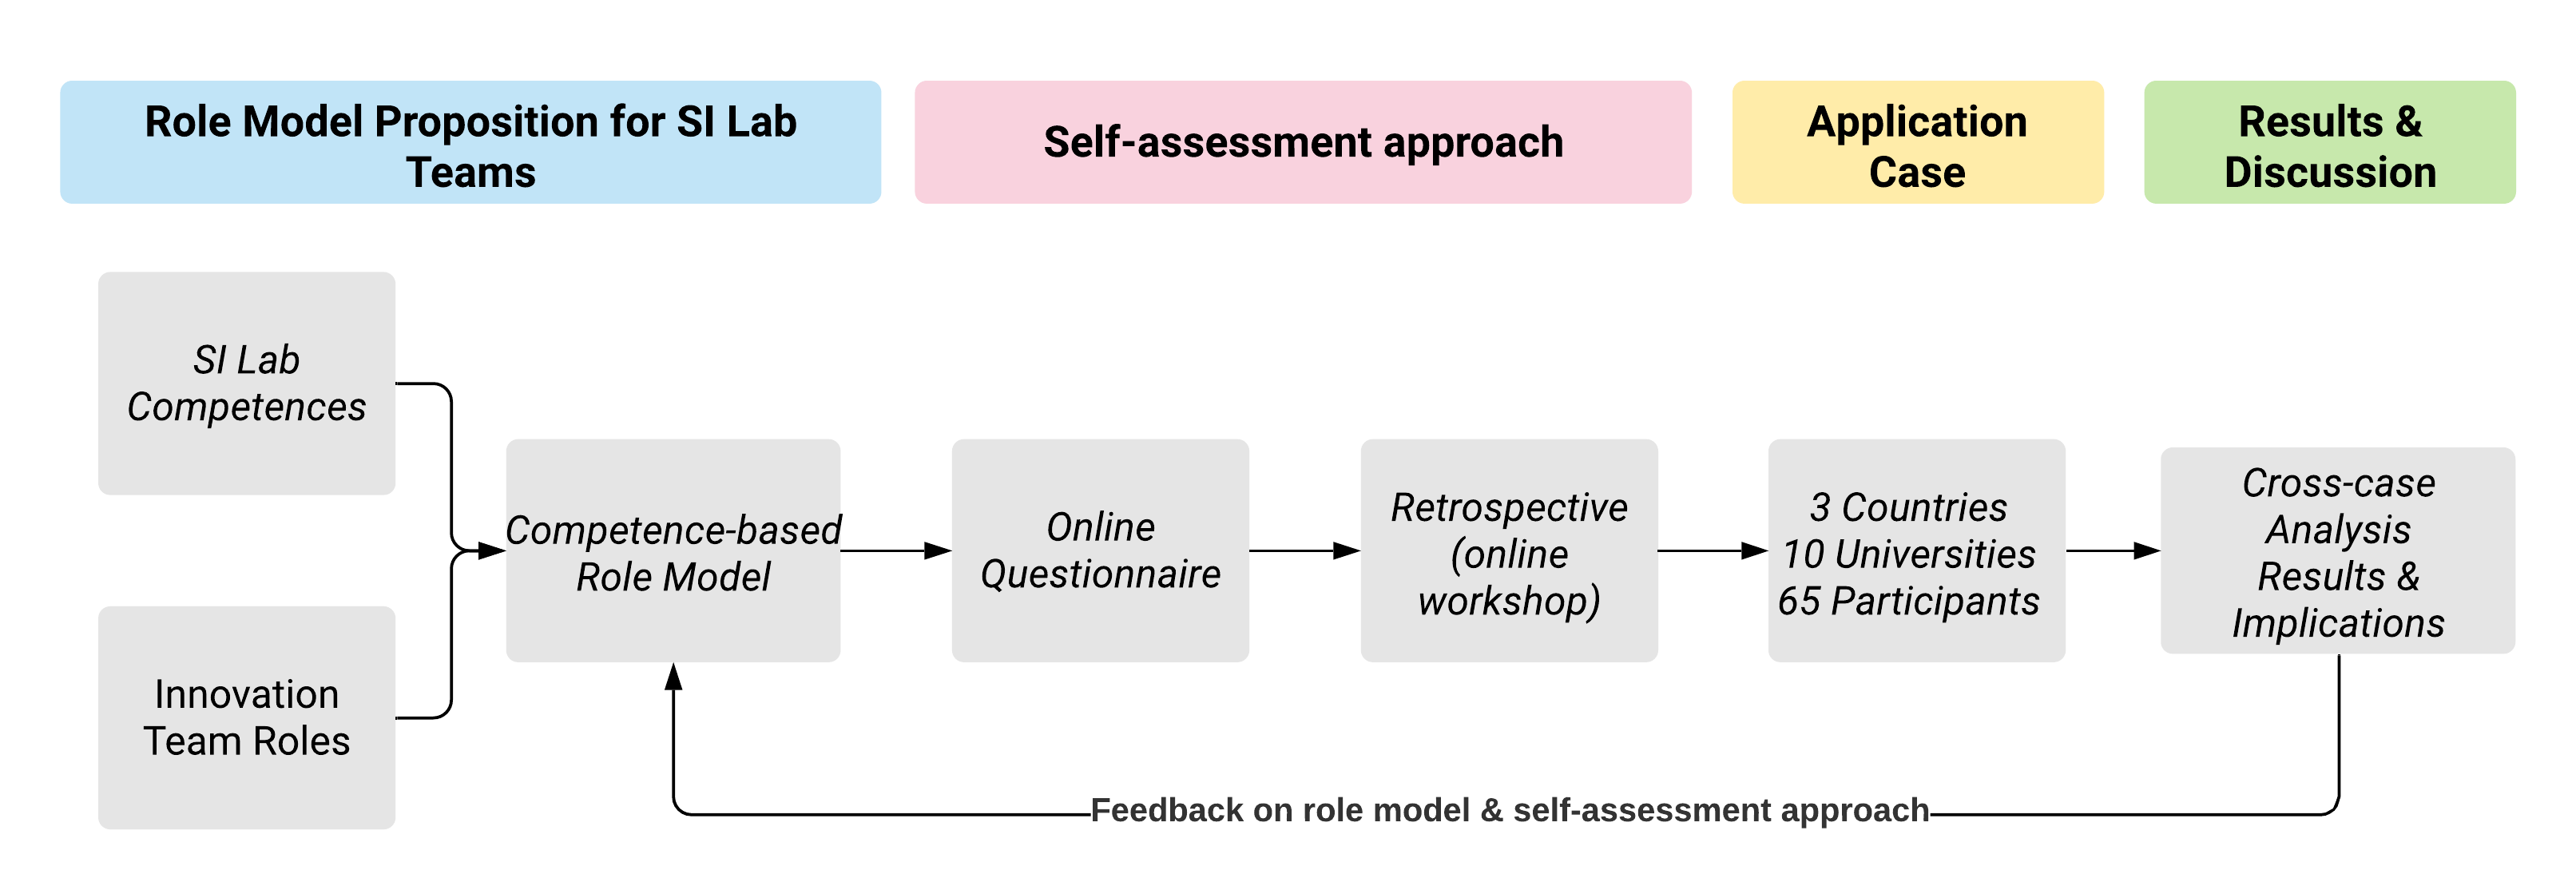
\includegraphics[width=0.95\linewidth]{Figures/Figure 1 - Methodology} 

}

\caption{Methodology overview}\label{fig:fig1}
\end{figure}

\hypertarget{proposition-of-a-competence-based-role-model-for-si-lab-teams}{%
\section{Proposition of a competence-based role model for SI Lab
teams}\label{proposition-of-a-competence-based-role-model-for-si-lab-teams}}

Despite several insights from empirical studies and different statements
regarding which functions or behaviors are possibly found in an
innovation team, propositions and explanations fall short of
expectations when it comes to the specificity of innovation lab teams.
Therefore, we have reason to believe that by establishing a clearer
connection between competences for SI labs and innovation team theory a
model can be proposed. First, drawing from the 14 competences proposed
by (\protect\hyperlink{ref-Wascher2018}{Wascher et al. 2018}), we
established a categorization according to the main functions that could
be set forth. Based on the literature and according to the authors'
knowledge and experience, four competence categories were identified, as
illustrated in Table 3. This was done in consideration of the
competences that most contribute to one of the following functions: (1)
innovation process orchestration, (2) materialize systemic solutions,
(3) spark connections and new ideas, and those that contribute to (4)
organizing and measuring results.

\providecommand{\docline}[3]{\noalign{\global\setlength{\arrayrulewidth}{#1}}\arrayrulecolor[HTML]{#2}\cline{#3}}

\setlength{\tabcolsep}{2pt}

\renewcommand*{\arraystretch}{1.5}

\begin{longtable}[c]{|p{1.00in}|p{0.80in}|p{0.80in}|p{0.80in}|p{0.80in}}

\caption{Categorization of SI lab team competences
}\\

\hhline{~~~~~}

\multicolumn{1}{!{\color[HTML]{000000}\vrule width 0pt}>{\cellcolor[HTML]{CFCFCF}\raggedright}p{\dimexpr 1in+0\tabcolsep+0\arrayrulewidth}}{\fontsize{8}{8}\selectfont{\textcolor[HTML]{000000}{\textbf{Competence}}}} & \multicolumn{1}{!{\color[HTML]{000000}\vrule width 0pt}>{\cellcolor[HTML]{CFCFCF}\raggedright}p{\dimexpr 0.8in+0\tabcolsep+0\arrayrulewidth}}{\fontsize{8}{8}\selectfont{\textcolor[HTML]{000000}{\textbf{Orchestrate\ Innovation\ Process}}}} & \multicolumn{1}{!{\color[HTML]{000000}\vrule width 0pt}>{\cellcolor[HTML]{CFCFCF}\raggedright}p{\dimexpr 0.8in+0\tabcolsep+0\arrayrulewidth}}{\fontsize{8}{8}\selectfont{\textcolor[HTML]{000000}{\textbf{Materialize\ Systemic\ Solutions}}}} & \multicolumn{1}{!{\color[HTML]{000000}\vrule width 0pt}>{\cellcolor[HTML]{CFCFCF}\raggedright}p{\dimexpr 0.8in+0\tabcolsep+0\arrayrulewidth}}{\fontsize{8}{8}\selectfont{\textcolor[HTML]{000000}{\textbf{Spark\ Connections\ \&\ Ideas}}}} & \multicolumn{1}{!{\color[HTML]{000000}\vrule width 0pt}>{\cellcolor[HTML]{CFCFCF}\raggedright}p{\dimexpr 0.8in+0\tabcolsep+0\arrayrulewidth}!{\color[HTML]{000000}\vrule width 0pt}}{\fontsize{8}{8}\selectfont{\textcolor[HTML]{000000}{\textbf{Organize\ and\ measure\ results}}}} \\



\endfirsthead

\hhline{~~~~~}

\multicolumn{1}{!{\color[HTML]{000000}\vrule width 0pt}>{\cellcolor[HTML]{CFCFCF}\raggedright}p{\dimexpr 1in+0\tabcolsep+0\arrayrulewidth}}{\fontsize{8}{8}\selectfont{\textcolor[HTML]{000000}{\textbf{Competence}}}} & \multicolumn{1}{!{\color[HTML]{000000}\vrule width 0pt}>{\cellcolor[HTML]{CFCFCF}\raggedright}p{\dimexpr 0.8in+0\tabcolsep+0\arrayrulewidth}}{\fontsize{8}{8}\selectfont{\textcolor[HTML]{000000}{\textbf{Orchestrate\ Innovation\ Process}}}} & \multicolumn{1}{!{\color[HTML]{000000}\vrule width 0pt}>{\cellcolor[HTML]{CFCFCF}\raggedright}p{\dimexpr 0.8in+0\tabcolsep+0\arrayrulewidth}}{\fontsize{8}{8}\selectfont{\textcolor[HTML]{000000}{\textbf{Materialize\ Systemic\ Solutions}}}} & \multicolumn{1}{!{\color[HTML]{000000}\vrule width 0pt}>{\cellcolor[HTML]{CFCFCF}\raggedright}p{\dimexpr 0.8in+0\tabcolsep+0\arrayrulewidth}}{\fontsize{8}{8}\selectfont{\textcolor[HTML]{000000}{\textbf{Spark\ Connections\ \&\ Ideas}}}} & \multicolumn{1}{!{\color[HTML]{000000}\vrule width 0pt}>{\cellcolor[HTML]{CFCFCF}\raggedright}p{\dimexpr 0.8in+0\tabcolsep+0\arrayrulewidth}!{\color[HTML]{000000}\vrule width 0pt}}{\fontsize{8}{8}\selectfont{\textcolor[HTML]{000000}{\textbf{Organize\ and\ measure\ results}}}} \\

\endhead



\multicolumn{1}{!{\color[HTML]{000000}\vrule width 0pt}>{\cellcolor[HTML]{EFEFEF}\raggedright}p{\dimexpr 1in+0\tabcolsep+0\arrayrulewidth}}{\fontsize{8}{8}\selectfont{\textcolor[HTML]{000000}{Project\ management}}} & \multicolumn{1}{!{\color[HTML]{000000}\vrule width 0pt}>{\cellcolor[HTML]{EFEFEF}\raggedright}p{\dimexpr 0.8in+0\tabcolsep+0\arrayrulewidth}}{\fontsize{8}{8}\selectfont{\textcolor[HTML]{000000}{}}} & \multicolumn{1}{!{\color[HTML]{000000}\vrule width 0pt}>{\cellcolor[HTML]{EFEFEF}\raggedright}p{\dimexpr 0.8in+0\tabcolsep+0\arrayrulewidth}}{\fontsize{8}{8}\selectfont{\textcolor[HTML]{000000}{}}} & \multicolumn{1}{!{\color[HTML]{000000}\vrule width 0pt}>{\cellcolor[HTML]{EFEFEF}\raggedright}p{\dimexpr 0.8in+0\tabcolsep+0\arrayrulewidth}}{\fontsize{8}{8}\selectfont{\textcolor[HTML]{000000}{}}} & \multicolumn{1}{!{\color[HTML]{000000}\vrule width 0pt}>{\cellcolor[HTML]{EFEFEF}\raggedright}p{\dimexpr 0.8in+0\tabcolsep+0\arrayrulewidth}!{\color[HTML]{000000}\vrule width 0pt}}{\fontsize{8}{8}\selectfont{\textcolor[HTML]{000000}{X}}} \\





\multicolumn{1}{!{\color[HTML]{000000}\vrule width 0pt}>{\raggedright}p{\dimexpr 1in+0\tabcolsep+0\arrayrulewidth}}{\fontsize{8}{8}\selectfont{\textcolor[HTML]{000000}{Moderation}}} & \multicolumn{1}{!{\color[HTML]{000000}\vrule width 0pt}>{\raggedright}p{\dimexpr 0.8in+0\tabcolsep+0\arrayrulewidth}}{\fontsize{8}{8}\selectfont{\textcolor[HTML]{000000}{X}}} & \multicolumn{1}{!{\color[HTML]{000000}\vrule width 0pt}>{\raggedright}p{\dimexpr 0.8in+0\tabcolsep+0\arrayrulewidth}}{\fontsize{8}{8}\selectfont{\textcolor[HTML]{000000}{}}} & \multicolumn{1}{!{\color[HTML]{000000}\vrule width 0pt}>{\raggedright}p{\dimexpr 0.8in+0\tabcolsep+0\arrayrulewidth}}{\fontsize{8}{8}\selectfont{\textcolor[HTML]{000000}{}}} & \multicolumn{1}{!{\color[HTML]{000000}\vrule width 0pt}>{\raggedright}p{\dimexpr 0.8in+0\tabcolsep+0\arrayrulewidth}!{\color[HTML]{000000}\vrule width 0pt}}{\fontsize{8}{8}\selectfont{\textcolor[HTML]{000000}{}}} \\





\multicolumn{1}{!{\color[HTML]{000000}\vrule width 0pt}>{\cellcolor[HTML]{EFEFEF}\raggedright}p{\dimexpr 1in+0\tabcolsep+0\arrayrulewidth}}{\fontsize{8}{8}\selectfont{\textcolor[HTML]{000000}{Mediation}}} & \multicolumn{1}{!{\color[HTML]{000000}\vrule width 0pt}>{\cellcolor[HTML]{EFEFEF}\raggedright}p{\dimexpr 0.8in+0\tabcolsep+0\arrayrulewidth}}{\fontsize{8}{8}\selectfont{\textcolor[HTML]{000000}{X}}} & \multicolumn{1}{!{\color[HTML]{000000}\vrule width 0pt}>{\cellcolor[HTML]{EFEFEF}\raggedright}p{\dimexpr 0.8in+0\tabcolsep+0\arrayrulewidth}}{\fontsize{8}{8}\selectfont{\textcolor[HTML]{000000}{}}} & \multicolumn{1}{!{\color[HTML]{000000}\vrule width 0pt}>{\cellcolor[HTML]{EFEFEF}\raggedright}p{\dimexpr 0.8in+0\tabcolsep+0\arrayrulewidth}}{\fontsize{8}{8}\selectfont{\textcolor[HTML]{000000}{}}} & \multicolumn{1}{!{\color[HTML]{000000}\vrule width 0pt}>{\cellcolor[HTML]{EFEFEF}\raggedright}p{\dimexpr 0.8in+0\tabcolsep+0\arrayrulewidth}!{\color[HTML]{000000}\vrule width 0pt}}{\fontsize{8}{8}\selectfont{\textcolor[HTML]{000000}{}}} \\





\multicolumn{1}{!{\color[HTML]{000000}\vrule width 0pt}>{\raggedright}p{\dimexpr 1in+0\tabcolsep+0\arrayrulewidth}}{\fontsize{8}{8}\selectfont{\textcolor[HTML]{000000}{Networking}}} & \multicolumn{1}{!{\color[HTML]{000000}\vrule width 0pt}>{\raggedright}p{\dimexpr 0.8in+0\tabcolsep+0\arrayrulewidth}}{\fontsize{8}{8}\selectfont{\textcolor[HTML]{000000}{}}} & \multicolumn{1}{!{\color[HTML]{000000}\vrule width 0pt}>{\raggedright}p{\dimexpr 0.8in+0\tabcolsep+0\arrayrulewidth}}{\fontsize{8}{8}\selectfont{\textcolor[HTML]{000000}{}}} & \multicolumn{1}{!{\color[HTML]{000000}\vrule width 0pt}>{\raggedright}p{\dimexpr 0.8in+0\tabcolsep+0\arrayrulewidth}}{\fontsize{8}{8}\selectfont{\textcolor[HTML]{000000}{X}}} & \multicolumn{1}{!{\color[HTML]{000000}\vrule width 0pt}>{\raggedright}p{\dimexpr 0.8in+0\tabcolsep+0\arrayrulewidth}!{\color[HTML]{000000}\vrule width 0pt}}{\fontsize{8}{8}\selectfont{\textcolor[HTML]{000000}{}}} \\





\multicolumn{1}{!{\color[HTML]{000000}\vrule width 0pt}>{\cellcolor[HTML]{EFEFEF}\raggedright}p{\dimexpr 1in+0\tabcolsep+0\arrayrulewidth}}{\fontsize{8}{8}\selectfont{\textcolor[HTML]{000000}{Participation}}} & \multicolumn{1}{!{\color[HTML]{000000}\vrule width 0pt}>{\cellcolor[HTML]{EFEFEF}\raggedright}p{\dimexpr 0.8in+0\tabcolsep+0\arrayrulewidth}}{\fontsize{8}{8}\selectfont{\textcolor[HTML]{000000}{X}}} & \multicolumn{1}{!{\color[HTML]{000000}\vrule width 0pt}>{\cellcolor[HTML]{EFEFEF}\raggedright}p{\dimexpr 0.8in+0\tabcolsep+0\arrayrulewidth}}{\fontsize{8}{8}\selectfont{\textcolor[HTML]{000000}{}}} & \multicolumn{1}{!{\color[HTML]{000000}\vrule width 0pt}>{\cellcolor[HTML]{EFEFEF}\raggedright}p{\dimexpr 0.8in+0\tabcolsep+0\arrayrulewidth}}{\fontsize{8}{8}\selectfont{\textcolor[HTML]{000000}{}}} & \multicolumn{1}{!{\color[HTML]{000000}\vrule width 0pt}>{\cellcolor[HTML]{EFEFEF}\raggedright}p{\dimexpr 0.8in+0\tabcolsep+0\arrayrulewidth}!{\color[HTML]{000000}\vrule width 0pt}}{\fontsize{8}{8}\selectfont{\textcolor[HTML]{000000}{}}} \\





\multicolumn{1}{!{\color[HTML]{000000}\vrule width 0pt}>{\raggedright}p{\dimexpr 1in+0\tabcolsep+0\arrayrulewidth}}{\fontsize{8}{8}\selectfont{\textcolor[HTML]{000000}{Communication}}} & \multicolumn{1}{!{\color[HTML]{000000}\vrule width 0pt}>{\raggedright}p{\dimexpr 0.8in+0\tabcolsep+0\arrayrulewidth}}{\fontsize{8}{8}\selectfont{\textcolor[HTML]{000000}{}}} & \multicolumn{1}{!{\color[HTML]{000000}\vrule width 0pt}>{\raggedright}p{\dimexpr 0.8in+0\tabcolsep+0\arrayrulewidth}}{\fontsize{8}{8}\selectfont{\textcolor[HTML]{000000}{}}} & \multicolumn{1}{!{\color[HTML]{000000}\vrule width 0pt}>{\raggedright}p{\dimexpr 0.8in+0\tabcolsep+0\arrayrulewidth}}{\fontsize{8}{8}\selectfont{\textcolor[HTML]{000000}{X}}} & \multicolumn{1}{!{\color[HTML]{000000}\vrule width 0pt}>{\raggedright}p{\dimexpr 0.8in+0\tabcolsep+0\arrayrulewidth}!{\color[HTML]{000000}\vrule width 0pt}}{\fontsize{8}{8}\selectfont{\textcolor[HTML]{000000}{}}} \\





\multicolumn{1}{!{\color[HTML]{000000}\vrule width 0pt}>{\cellcolor[HTML]{EFEFEF}\raggedright}p{\dimexpr 1in+0\tabcolsep+0\arrayrulewidth}}{\fontsize{8}{8}\selectfont{\textcolor[HTML]{000000}{Self-organization}}} & \multicolumn{1}{!{\color[HTML]{000000}\vrule width 0pt}>{\cellcolor[HTML]{EFEFEF}\raggedright}p{\dimexpr 0.8in+0\tabcolsep+0\arrayrulewidth}}{\fontsize{8}{8}\selectfont{\textcolor[HTML]{000000}{}}} & \multicolumn{1}{!{\color[HTML]{000000}\vrule width 0pt}>{\cellcolor[HTML]{EFEFEF}\raggedright}p{\dimexpr 0.8in+0\tabcolsep+0\arrayrulewidth}}{\fontsize{8}{8}\selectfont{\textcolor[HTML]{000000}{}}} & \multicolumn{1}{!{\color[HTML]{000000}\vrule width 0pt}>{\cellcolor[HTML]{EFEFEF}\raggedright}p{\dimexpr 0.8in+0\tabcolsep+0\arrayrulewidth}}{\fontsize{8}{8}\selectfont{\textcolor[HTML]{000000}{}}} & \multicolumn{1}{!{\color[HTML]{000000}\vrule width 0pt}>{\cellcolor[HTML]{EFEFEF}\raggedright}p{\dimexpr 0.8in+0\tabcolsep+0\arrayrulewidth}!{\color[HTML]{000000}\vrule width 0pt}}{\fontsize{8}{8}\selectfont{\textcolor[HTML]{000000}{X}}} \\





\multicolumn{1}{!{\color[HTML]{000000}\vrule width 0pt}>{\raggedright}p{\dimexpr 1in+0\tabcolsep+0\arrayrulewidth}}{\fontsize{8}{8}\selectfont{\textcolor[HTML]{000000}{Intercultural}}} & \multicolumn{1}{!{\color[HTML]{000000}\vrule width 0pt}>{\raggedright}p{\dimexpr 0.8in+0\tabcolsep+0\arrayrulewidth}}{\fontsize{8}{8}\selectfont{\textcolor[HTML]{000000}{X}}} & \multicolumn{1}{!{\color[HTML]{000000}\vrule width 0pt}>{\raggedright}p{\dimexpr 0.8in+0\tabcolsep+0\arrayrulewidth}}{\fontsize{8}{8}\selectfont{\textcolor[HTML]{000000}{}}} & \multicolumn{1}{!{\color[HTML]{000000}\vrule width 0pt}>{\raggedright}p{\dimexpr 0.8in+0\tabcolsep+0\arrayrulewidth}}{\fontsize{8}{8}\selectfont{\textcolor[HTML]{000000}{}}} & \multicolumn{1}{!{\color[HTML]{000000}\vrule width 0pt}>{\raggedright}p{\dimexpr 0.8in+0\tabcolsep+0\arrayrulewidth}!{\color[HTML]{000000}\vrule width 0pt}}{\fontsize{8}{8}\selectfont{\textcolor[HTML]{000000}{}}} \\





\multicolumn{1}{!{\color[HTML]{000000}\vrule width 0pt}>{\cellcolor[HTML]{EFEFEF}\raggedright}p{\dimexpr 1in+0\tabcolsep+0\arrayrulewidth}}{\fontsize{8}{8}\selectfont{\textcolor[HTML]{000000}{Evaluation}}} & \multicolumn{1}{!{\color[HTML]{000000}\vrule width 0pt}>{\cellcolor[HTML]{EFEFEF}\raggedright}p{\dimexpr 0.8in+0\tabcolsep+0\arrayrulewidth}}{\fontsize{8}{8}\selectfont{\textcolor[HTML]{000000}{}}} & \multicolumn{1}{!{\color[HTML]{000000}\vrule width 0pt}>{\cellcolor[HTML]{EFEFEF}\raggedright}p{\dimexpr 0.8in+0\tabcolsep+0\arrayrulewidth}}{\fontsize{8}{8}\selectfont{\textcolor[HTML]{000000}{}}} & \multicolumn{1}{!{\color[HTML]{000000}\vrule width 0pt}>{\cellcolor[HTML]{EFEFEF}\raggedright}p{\dimexpr 0.8in+0\tabcolsep+0\arrayrulewidth}}{\fontsize{8}{8}\selectfont{\textcolor[HTML]{000000}{}}} & \multicolumn{1}{!{\color[HTML]{000000}\vrule width 0pt}>{\cellcolor[HTML]{EFEFEF}\raggedright}p{\dimexpr 0.8in+0\tabcolsep+0\arrayrulewidth}!{\color[HTML]{000000}\vrule width 0pt}}{\fontsize{8}{8}\selectfont{\textcolor[HTML]{000000}{X}}} \\





\multicolumn{1}{!{\color[HTML]{000000}\vrule width 0pt}>{\raggedright}p{\dimexpr 1in+0\tabcolsep+0\arrayrulewidth}}{\fontsize{8}{8}\selectfont{\textcolor[HTML]{000000}{Research\ methods\ and\ interdisciplinary\ work}}} & \multicolumn{1}{!{\color[HTML]{000000}\vrule width 0pt}>{\raggedright}p{\dimexpr 0.8in+0\tabcolsep+0\arrayrulewidth}}{\fontsize{8}{8}\selectfont{\textcolor[HTML]{000000}{}}} & \multicolumn{1}{!{\color[HTML]{000000}\vrule width 0pt}>{\raggedright}p{\dimexpr 0.8in+0\tabcolsep+0\arrayrulewidth}}{\fontsize{8}{8}\selectfont{\textcolor[HTML]{000000}{X}}} & \multicolumn{1}{!{\color[HTML]{000000}\vrule width 0pt}>{\raggedright}p{\dimexpr 0.8in+0\tabcolsep+0\arrayrulewidth}}{\fontsize{8}{8}\selectfont{\textcolor[HTML]{000000}{}}} & \multicolumn{1}{!{\color[HTML]{000000}\vrule width 0pt}>{\raggedright}p{\dimexpr 0.8in+0\tabcolsep+0\arrayrulewidth}!{\color[HTML]{000000}\vrule width 0pt}}{\fontsize{8}{8}\selectfont{\textcolor[HTML]{000000}{}}} \\





\multicolumn{1}{!{\color[HTML]{000000}\vrule width 0pt}>{\cellcolor[HTML]{EFEFEF}\raggedright}p{\dimexpr 1in+0\tabcolsep+0\arrayrulewidth}}{\fontsize{8}{8}\selectfont{\textcolor[HTML]{000000}{Design\ methods\ and\ creative\ thinking}}} & \multicolumn{1}{!{\color[HTML]{000000}\vrule width 0pt}>{\cellcolor[HTML]{EFEFEF}\raggedright}p{\dimexpr 0.8in+0\tabcolsep+0\arrayrulewidth}}{\fontsize{8}{8}\selectfont{\textcolor[HTML]{000000}{}}} & \multicolumn{1}{!{\color[HTML]{000000}\vrule width 0pt}>{\cellcolor[HTML]{EFEFEF}\raggedright}p{\dimexpr 0.8in+0\tabcolsep+0\arrayrulewidth}}{\fontsize{8}{8}\selectfont{\textcolor[HTML]{000000}{X}}} & \multicolumn{1}{!{\color[HTML]{000000}\vrule width 0pt}>{\cellcolor[HTML]{EFEFEF}\raggedright}p{\dimexpr 0.8in+0\tabcolsep+0\arrayrulewidth}}{\fontsize{8}{8}\selectfont{\textcolor[HTML]{000000}{}}} & \multicolumn{1}{!{\color[HTML]{000000}\vrule width 0pt}>{\cellcolor[HTML]{EFEFEF}\raggedright}p{\dimexpr 0.8in+0\tabcolsep+0\arrayrulewidth}!{\color[HTML]{000000}\vrule width 0pt}}{\fontsize{8}{8}\selectfont{\textcolor[HTML]{000000}{}}} \\





\multicolumn{1}{!{\color[HTML]{000000}\vrule width 0pt}>{\raggedright}p{\dimexpr 1in+0\tabcolsep+0\arrayrulewidth}}{\fontsize{8}{8}\selectfont{\textcolor[HTML]{000000}{Information\ and\ telecommunication\ techniques}}} & \multicolumn{1}{!{\color[HTML]{000000}\vrule width 0pt}>{\raggedright}p{\dimexpr 0.8in+0\tabcolsep+0\arrayrulewidth}}{\fontsize{8}{8}\selectfont{\textcolor[HTML]{000000}{}}} & \multicolumn{1}{!{\color[HTML]{000000}\vrule width 0pt}>{\raggedright}p{\dimexpr 0.8in+0\tabcolsep+0\arrayrulewidth}}{\fontsize{8}{8}\selectfont{\textcolor[HTML]{000000}{X}}} & \multicolumn{1}{!{\color[HTML]{000000}\vrule width 0pt}>{\raggedright}p{\dimexpr 0.8in+0\tabcolsep+0\arrayrulewidth}}{\fontsize{8}{8}\selectfont{\textcolor[HTML]{000000}{}}} & \multicolumn{1}{!{\color[HTML]{000000}\vrule width 0pt}>{\raggedright}p{\dimexpr 0.8in+0\tabcolsep+0\arrayrulewidth}!{\color[HTML]{000000}\vrule width 0pt}}{\fontsize{8}{8}\selectfont{\textcolor[HTML]{000000}{}}} \\





\multicolumn{1}{!{\color[HTML]{000000}\vrule width 0pt}>{\cellcolor[HTML]{EFEFEF}\raggedright}p{\dimexpr 1in+0\tabcolsep+0\arrayrulewidth}}{\fontsize{8}{8}\selectfont{\textcolor[HTML]{000000}{Entrepreneurial\ thinking}}} & \multicolumn{1}{!{\color[HTML]{000000}\vrule width 0pt}>{\cellcolor[HTML]{EFEFEF}\raggedright}p{\dimexpr 0.8in+0\tabcolsep+0\arrayrulewidth}}{\fontsize{8}{8}\selectfont{\textcolor[HTML]{000000}{}}} & \multicolumn{1}{!{\color[HTML]{000000}\vrule width 0pt}>{\cellcolor[HTML]{EFEFEF}\raggedright}p{\dimexpr 0.8in+0\tabcolsep+0\arrayrulewidth}}{\fontsize{8}{8}\selectfont{\textcolor[HTML]{000000}{}}} & \multicolumn{1}{!{\color[HTML]{000000}\vrule width 0pt}>{\cellcolor[HTML]{EFEFEF}\raggedright}p{\dimexpr 0.8in+0\tabcolsep+0\arrayrulewidth}}{\fontsize{8}{8}\selectfont{\textcolor[HTML]{000000}{X}}} & \multicolumn{1}{!{\color[HTML]{000000}\vrule width 0pt}>{\cellcolor[HTML]{EFEFEF}\raggedright}p{\dimexpr 0.8in+0\tabcolsep+0\arrayrulewidth}!{\color[HTML]{000000}\vrule width 0pt}}{\fontsize{8}{8}\selectfont{\textcolor[HTML]{000000}{}}} \\





\multicolumn{1}{!{\color[HTML]{000000}\vrule width 0pt}>{\raggedright}p{\dimexpr 1in+0\tabcolsep+0\arrayrulewidth}}{\fontsize{8}{8}\selectfont{\textcolor[HTML]{000000}{Systems\ thinking}}} & \multicolumn{1}{!{\color[HTML]{000000}\vrule width 0pt}>{\raggedright}p{\dimexpr 0.8in+0\tabcolsep+0\arrayrulewidth}}{\fontsize{8}{8}\selectfont{\textcolor[HTML]{000000}{}}} & \multicolumn{1}{!{\color[HTML]{000000}\vrule width 0pt}>{\raggedright}p{\dimexpr 0.8in+0\tabcolsep+0\arrayrulewidth}}{\fontsize{8}{8}\selectfont{\textcolor[HTML]{000000}{X}}} & \multicolumn{1}{!{\color[HTML]{000000}\vrule width 0pt}>{\raggedright}p{\dimexpr 0.8in+0\tabcolsep+0\arrayrulewidth}}{\fontsize{8}{8}\selectfont{\textcolor[HTML]{000000}{}}} & \multicolumn{1}{!{\color[HTML]{000000}\vrule width 0pt}>{\raggedright}p{\dimexpr 0.8in+0\tabcolsep+0\arrayrulewidth}!{\color[HTML]{000000}\vrule width 0pt}}{\fontsize{8}{8}\selectfont{\textcolor[HTML]{000000}{}}} \\





\end{longtable}

Then, in order to gain a finer sense of how to better define these
competences for innovation teams and their roles, we compared the four
competence categories to the innovation roles found in the literature.
At this point, we looked for similarities between the roles and
behaviors that were historically recognized among innovation teams and
the competences for SI labs. We found that all four categories were
present in the seven innovation team role models (see Table 4). It is
worth remembering that our focus for this study is the composition of
lab teams. This means that while proceeding to this comparison our
attention remained focused on the roles at the core of innovation lab
management. This is why a fifth category emerges as ``external roles'',
which refer to users or external parties that revolve around the network
of lab stakeholders. By no means is our intent to diminish the
importance of these roles, on the contrary, we would like to mention
that these external roles should definitely be studied in depth at the
further stages of the research. However, considering the usually
relatively small size of innovation lab teams, especially in the early
stages, we believe that these four categories constitute a comprehensive
and pragmatic basis for this study.

\providecommand{\docline}[3]{\noalign{\global\setlength{\arrayrulewidth}{#1}}\arrayrulecolor[HTML]{#2}\cline{#3}}

\setlength{\tabcolsep}{2pt}

\renewcommand*{\arraystretch}{1.5}

\begin{longtable}[c]{|p{1.20in}|p{1.00in}|p{1.00in}|p{1.00in}|p{1.00in}|p{1.00in}}

\caption{Innovation Role Model Comparison
}\\

\hhline{>{\arrayrulecolor[HTML]{666666}\global\arrayrulewidth=2pt}->{\arrayrulecolor[HTML]{666666}\global\arrayrulewidth=2pt}->{\arrayrulecolor[HTML]{666666}\global\arrayrulewidth=2pt}->{\arrayrulecolor[HTML]{666666}\global\arrayrulewidth=2pt}->{\arrayrulecolor[HTML]{666666}\global\arrayrulewidth=2pt}->{\arrayrulecolor[HTML]{666666}\global\arrayrulewidth=2pt}-}

\multicolumn{1}{!{\color[HTML]{000000}\vrule width 0pt}>{\raggedright}p{\dimexpr 1.2in+0\tabcolsep+0\arrayrulewidth}}{\fontsize{9}{9}\selectfont{\textcolor[HTML]{000000}{Reference}}} & \multicolumn{1}{!{\color[HTML]{000000}\vrule width 0pt}>{\raggedright}p{\dimexpr 1in+0\tabcolsep+0\arrayrulewidth}}{\fontsize{9}{9}\selectfont{\textcolor[HTML]{000000}{Orchestrate\ Innovation\ Processes}}} & \multicolumn{1}{!{\color[HTML]{000000}\vrule width 0pt}>{\raggedright}p{\dimexpr 1in+0\tabcolsep+0\arrayrulewidth}}{\fontsize{9}{9}\selectfont{\textcolor[HTML]{000000}{Materialize\ Systemic\ Solutions}}} & \multicolumn{1}{!{\color[HTML]{000000}\vrule width 0pt}>{\raggedright}p{\dimexpr 1in+0\tabcolsep+0\arrayrulewidth}}{\fontsize{9}{9}\selectfont{\textcolor[HTML]{000000}{Spark\ Connections\ \&\ Ideas}}} & \multicolumn{1}{!{\color[HTML]{000000}\vrule width 0pt}>{\raggedright}p{\dimexpr 1in+0\tabcolsep+0\arrayrulewidth}}{\fontsize{9}{9}\selectfont{\textcolor[HTML]{000000}{Organize\ and\ measure\ results}}} & \multicolumn{1}{!{\color[HTML]{000000}\vrule width 0pt}>{\raggedright}p{\dimexpr 1in+0\tabcolsep+0\arrayrulewidth}!{\color[HTML]{000000}\vrule width 0pt}}{\fontsize{9}{9}\selectfont{\textcolor[HTML]{000000}{External\ Roles}}} \\

\hhline{>{\arrayrulecolor[HTML]{666666}\global\arrayrulewidth=2pt}->{\arrayrulecolor[HTML]{666666}\global\arrayrulewidth=2pt}->{\arrayrulecolor[HTML]{666666}\global\arrayrulewidth=2pt}->{\arrayrulecolor[HTML]{666666}\global\arrayrulewidth=2pt}->{\arrayrulecolor[HTML]{666666}\global\arrayrulewidth=2pt}->{\arrayrulecolor[HTML]{666666}\global\arrayrulewidth=2pt}-}

\endfirsthead

\hhline{>{\arrayrulecolor[HTML]{666666}\global\arrayrulewidth=2pt}->{\arrayrulecolor[HTML]{666666}\global\arrayrulewidth=2pt}->{\arrayrulecolor[HTML]{666666}\global\arrayrulewidth=2pt}->{\arrayrulecolor[HTML]{666666}\global\arrayrulewidth=2pt}->{\arrayrulecolor[HTML]{666666}\global\arrayrulewidth=2pt}->{\arrayrulecolor[HTML]{666666}\global\arrayrulewidth=2pt}-}

\multicolumn{1}{!{\color[HTML]{000000}\vrule width 0pt}>{\raggedright}p{\dimexpr 1.2in+0\tabcolsep+0\arrayrulewidth}}{\fontsize{9}{9}\selectfont{\textcolor[HTML]{000000}{Reference}}} & \multicolumn{1}{!{\color[HTML]{000000}\vrule width 0pt}>{\raggedright}p{\dimexpr 1in+0\tabcolsep+0\arrayrulewidth}}{\fontsize{9}{9}\selectfont{\textcolor[HTML]{000000}{Orchestrate\ Innovation\ Processes}}} & \multicolumn{1}{!{\color[HTML]{000000}\vrule width 0pt}>{\raggedright}p{\dimexpr 1in+0\tabcolsep+0\arrayrulewidth}}{\fontsize{9}{9}\selectfont{\textcolor[HTML]{000000}{Materialize\ Systemic\ Solutions}}} & \multicolumn{1}{!{\color[HTML]{000000}\vrule width 0pt}>{\raggedright}p{\dimexpr 1in+0\tabcolsep+0\arrayrulewidth}}{\fontsize{9}{9}\selectfont{\textcolor[HTML]{000000}{Spark\ Connections\ \&\ Ideas}}} & \multicolumn{1}{!{\color[HTML]{000000}\vrule width 0pt}>{\raggedright}p{\dimexpr 1in+0\tabcolsep+0\arrayrulewidth}}{\fontsize{9}{9}\selectfont{\textcolor[HTML]{000000}{Organize\ and\ measure\ results}}} & \multicolumn{1}{!{\color[HTML]{000000}\vrule width 0pt}>{\raggedright}p{\dimexpr 1in+0\tabcolsep+0\arrayrulewidth}!{\color[HTML]{000000}\vrule width 0pt}}{\fontsize{9}{9}\selectfont{\textcolor[HTML]{000000}{External\ Roles}}} \\

\hhline{>{\arrayrulecolor[HTML]{666666}\global\arrayrulewidth=2pt}->{\arrayrulecolor[HTML]{666666}\global\arrayrulewidth=2pt}->{\arrayrulecolor[HTML]{666666}\global\arrayrulewidth=2pt}->{\arrayrulecolor[HTML]{666666}\global\arrayrulewidth=2pt}->{\arrayrulecolor[HTML]{666666}\global\arrayrulewidth=2pt}->{\arrayrulecolor[HTML]{666666}\global\arrayrulewidth=2pt}-}\endhead



\multicolumn{1}{!{\color[HTML]{000000}\vrule width 0pt}>{\raggedright}p{\dimexpr 1.2in+0\tabcolsep+0\arrayrulewidth}}{\fontsize{9}{9}\selectfont{\textcolor[HTML]{000000}{Roberts\ \&\ Fusfeld.,\ 1982}}} & \multicolumn{1}{!{\color[HTML]{000000}\vrule width 0pt}>{\raggedright}p{\dimexpr 1in+0\tabcolsep+0\arrayrulewidth}}{\fontsize{9}{9}\selectfont{\textcolor[HTML]{000000}{-\ Sponsor\ or\ Coach}}} & \multicolumn{1}{!{\color[HTML]{000000}\vrule width 0pt}>{\raggedright}p{\dimexpr 1in+0\tabcolsep+0\arrayrulewidth}}{\fontsize{9}{9}\selectfont{\textcolor[HTML]{000000}{-\ Entrepreneur\ or\ Champion}}} & \multicolumn{1}{!{\color[HTML]{000000}\vrule width 0pt}>{\raggedright}p{\dimexpr 1in+0\tabcolsep+0\arrayrulewidth}}{\fontsize{9}{9}\selectfont{\textcolor[HTML]{000000}{-\ Idea\ Generator}}} & \multicolumn{1}{!{\color[HTML]{000000}\vrule width 0pt}>{\raggedright}p{\dimexpr 1in+0\tabcolsep+0\arrayrulewidth}}{\fontsize{9}{9}\selectfont{\textcolor[HTML]{000000}{-\ Project\ Leader}}} & \multicolumn{1}{!{\color[HTML]{000000}\vrule width 0pt}>{\raggedright}p{\dimexpr 1in+0\tabcolsep+0\arrayrulewidth}!{\color[HTML]{000000}\vrule width 0pt}}{\fontsize{9}{9}\selectfont{\textcolor[HTML]{000000}{}}} \\





\multicolumn{1}{!{\color[HTML]{000000}\vrule width 0pt}>{\raggedright}p{\dimexpr 1.2in+0\tabcolsep+0\arrayrulewidth}}{\fontsize{9}{9}\selectfont{\textcolor[HTML]{000000}{}}} & \multicolumn{1}{!{\color[HTML]{000000}\vrule width 0pt}>{\raggedright}p{\dimexpr 1in+0\tabcolsep+0\arrayrulewidth}}{\fontsize{9}{9}\selectfont{\textcolor[HTML]{000000}{}}} & \multicolumn{1}{!{\color[HTML]{000000}\vrule width 0pt}>{\raggedright}p{\dimexpr 1in+0\tabcolsep+0\arrayrulewidth}}{\fontsize{9}{9}\selectfont{\textcolor[HTML]{000000}{}}} & \multicolumn{1}{!{\color[HTML]{000000}\vrule width 0pt}>{\raggedright}p{\dimexpr 1in+0\tabcolsep+0\arrayrulewidth}}{\fontsize{9}{9}\selectfont{\textcolor[HTML]{000000}{}}} & \multicolumn{1}{!{\color[HTML]{000000}\vrule width 0pt}>{\raggedright}p{\dimexpr 1in+0\tabcolsep+0\arrayrulewidth}}{\fontsize{9}{9}\selectfont{\textcolor[HTML]{000000}{-\ Gatekeeper}}} & \multicolumn{1}{!{\color[HTML]{000000}\vrule width 0pt}>{\raggedright}p{\dimexpr 1in+0\tabcolsep+0\arrayrulewidth}!{\color[HTML]{000000}\vrule width 0pt}}{\fontsize{9}{9}\selectfont{\textcolor[HTML]{000000}{}}} \\

\hhline{>{\arrayrulecolor[HTML]{BEBEBE}\global\arrayrulewidth=0.1pt}->{\arrayrulecolor[HTML]{BEBEBE}\global\arrayrulewidth=0.1pt}->{\arrayrulecolor[HTML]{BEBEBE}\global\arrayrulewidth=0.1pt}->{\arrayrulecolor[HTML]{BEBEBE}\global\arrayrulewidth=0.1pt}->{\arrayrulecolor[HTML]{BEBEBE}\global\arrayrulewidth=0.1pt}->{\arrayrulecolor[HTML]{BEBEBE}\global\arrayrulewidth=0.1pt}-}



\multicolumn{1}{!{\color[HTML]{000000}\vrule width 0pt}>{\raggedright}p{\dimexpr 1.2in+0\tabcolsep+0\arrayrulewidth}}{\fontsize{9}{9}\selectfont{\textcolor[HTML]{000000}{Belbin,\ 2010\ (Originally\ published\ in\ 1993)}}} & \multicolumn{1}{!{\color[HTML]{000000}\vrule width 0pt}>{\raggedright}p{\dimexpr 1in+0\tabcolsep+0\arrayrulewidth}}{\fontsize{9}{9}\selectfont{\textcolor[HTML]{000000}{-\ Plant}}} & \multicolumn{1}{!{\color[HTML]{000000}\vrule width 0pt}>{\raggedright}p{\dimexpr 1in+0\tabcolsep+0\arrayrulewidth}}{\fontsize{9}{9}\selectfont{\textcolor[HTML]{000000}{-\ Implementer}}} & \multicolumn{1}{!{\color[HTML]{000000}\vrule width 0pt}>{\raggedright}p{\dimexpr 1in+0\tabcolsep+0\arrayrulewidth}}{\fontsize{9}{9}\selectfont{\textcolor[HTML]{000000}{-\ Resource\ Investigator}}} & \multicolumn{1}{!{\color[HTML]{000000}\vrule width 0pt}>{\raggedright}p{\dimexpr 1in+0\tabcolsep+0\arrayrulewidth}}{\fontsize{9}{9}\selectfont{\textcolor[HTML]{000000}{-\ Coordinator}}} & \multicolumn{1}{!{\color[HTML]{000000}\vrule width 0pt}>{\raggedright}p{\dimexpr 1in+0\tabcolsep+0\arrayrulewidth}!{\color[HTML]{000000}\vrule width 0pt}}{\fontsize{9}{9}\selectfont{\textcolor[HTML]{000000}{}}} \\





\multicolumn{1}{!{\color[HTML]{000000}\vrule width 0pt}>{\raggedright}p{\dimexpr 1.2in+0\tabcolsep+0\arrayrulewidth}}{\fontsize{9}{9}\selectfont{\textcolor[HTML]{000000}{}}} & \multicolumn{1}{!{\color[HTML]{000000}\vrule width 0pt}>{\raggedright}p{\dimexpr 1in+0\tabcolsep+0\arrayrulewidth}}{\fontsize{9}{9}\selectfont{\textcolor[HTML]{000000}{-\ Teamworker}}} & \multicolumn{1}{!{\color[HTML]{000000}\vrule width 0pt}>{\raggedright}p{\dimexpr 1in+0\tabcolsep+0\arrayrulewidth}}{\fontsize{9}{9}\selectfont{\textcolor[HTML]{000000}{-\ Specialist}}} & \multicolumn{1}{!{\color[HTML]{000000}\vrule width 0pt}>{\raggedright}p{\dimexpr 1in+0\tabcolsep+0\arrayrulewidth}}{\fontsize{9}{9}\selectfont{\textcolor[HTML]{000000}{-\ Shaper}}} & \multicolumn{1}{!{\color[HTML]{000000}\vrule width 0pt}>{\raggedright}p{\dimexpr 1in+0\tabcolsep+0\arrayrulewidth}}{\fontsize{9}{9}\selectfont{\textcolor[HTML]{000000}{-\ Monitor\ Evaluator}}} & \multicolumn{1}{!{\color[HTML]{000000}\vrule width 0pt}>{\raggedright}p{\dimexpr 1in+0\tabcolsep+0\arrayrulewidth}!{\color[HTML]{000000}\vrule width 0pt}}{\fontsize{9}{9}\selectfont{\textcolor[HTML]{000000}{}}} \\





\multicolumn{1}{!{\color[HTML]{000000}\vrule width 0pt}>{\raggedright}p{\dimexpr 1.2in+0\tabcolsep+0\arrayrulewidth}}{\fontsize{9}{9}\selectfont{\textcolor[HTML]{000000}{}}} & \multicolumn{1}{!{\color[HTML]{000000}\vrule width 0pt}>{\raggedright}p{\dimexpr 1in+0\tabcolsep+0\arrayrulewidth}}{\fontsize{9}{9}\selectfont{\textcolor[HTML]{000000}{}}} & \multicolumn{1}{!{\color[HTML]{000000}\vrule width 0pt}>{\raggedright}p{\dimexpr 1in+0\tabcolsep+0\arrayrulewidth}}{\fontsize{9}{9}\selectfont{\textcolor[HTML]{000000}{}}} & \multicolumn{1}{!{\color[HTML]{000000}\vrule width 0pt}>{\raggedright}p{\dimexpr 1in+0\tabcolsep+0\arrayrulewidth}}{\fontsize{9}{9}\selectfont{\textcolor[HTML]{000000}{}}} & \multicolumn{1}{!{\color[HTML]{000000}\vrule width 0pt}>{\raggedright}p{\dimexpr 1in+0\tabcolsep+0\arrayrulewidth}}{\fontsize{9}{9}\selectfont{\textcolor[HTML]{000000}{-\ Completer\ Finisher}}} & \multicolumn{1}{!{\color[HTML]{000000}\vrule width 0pt}>{\raggedright}p{\dimexpr 1in+0\tabcolsep+0\arrayrulewidth}!{\color[HTML]{000000}\vrule width 0pt}}{\fontsize{9}{9}\selectfont{\textcolor[HTML]{000000}{}}} \\

\hhline{>{\arrayrulecolor[HTML]{BEBEBE}\global\arrayrulewidth=0.1pt}->{\arrayrulecolor[HTML]{BEBEBE}\global\arrayrulewidth=0.1pt}->{\arrayrulecolor[HTML]{BEBEBE}\global\arrayrulewidth=0.1pt}->{\arrayrulecolor[HTML]{BEBEBE}\global\arrayrulewidth=0.1pt}->{\arrayrulecolor[HTML]{BEBEBE}\global\arrayrulewidth=0.1pt}->{\arrayrulecolor[HTML]{BEBEBE}\global\arrayrulewidth=0.1pt}-}



\multicolumn{1}{!{\color[HTML]{000000}\vrule width 0pt}>{\raggedright}p{\dimexpr 1.2in+0\tabcolsep+0\arrayrulewidth}}{\fontsize{9}{9}\selectfont{\textcolor[HTML]{000000}{Hering\ \&\ Phillips,\ 2005}}} & \multicolumn{1}{!{\color[HTML]{000000}\vrule width 0pt}>{\raggedright}p{\dimexpr 1in+0\tabcolsep+0\arrayrulewidth}}{\fontsize{9}{9}\selectfont{\textcolor[HTML]{000000}{-\ Framer}}} & \multicolumn{1}{!{\color[HTML]{000000}\vrule width 0pt}>{\raggedright}p{\dimexpr 1in+0\tabcolsep+0\arrayrulewidth}}{\fontsize{9}{9}\selectfont{\textcolor[HTML]{000000}{-\ Librarian}}} & \multicolumn{1}{!{\color[HTML]{000000}\vrule width 0pt}>{\raggedright}p{\dimexpr 1in+0\tabcolsep+0\arrayrulewidth}}{\fontsize{9}{9}\selectfont{\textcolor[HTML]{000000}{-\ Connector}}} & \multicolumn{1}{!{\color[HTML]{000000}\vrule width 0pt}>{\raggedright}p{\dimexpr 1in+0\tabcolsep+0\arrayrulewidth}}{\fontsize{9}{9}\selectfont{\textcolor[HTML]{000000}{-\ Judge}}} & \multicolumn{1}{!{\color[HTML]{000000}\vrule width 0pt}>{\raggedright}p{\dimexpr 1in+0\tabcolsep+0\arrayrulewidth}!{\color[HTML]{000000}\vrule width 0pt}}{\fontsize{9}{9}\selectfont{\textcolor[HTML]{000000}{}}} \\





\multicolumn{1}{!{\color[HTML]{000000}\vrule width 0pt}>{\raggedright}p{\dimexpr 1.2in+0\tabcolsep+0\arrayrulewidth}}{\fontsize{9}{9}\selectfont{\textcolor[HTML]{000000}{}}} & \multicolumn{1}{!{\color[HTML]{000000}\vrule width 0pt}>{\raggedright}p{\dimexpr 1in+0\tabcolsep+0\arrayrulewidth}}{\fontsize{9}{9}\selectfont{\textcolor[HTML]{000000}{}}} & \multicolumn{1}{!{\color[HTML]{000000}\vrule width 0pt}>{\raggedright}p{\dimexpr 1in+0\tabcolsep+0\arrayrulewidth}}{\fontsize{9}{9}\selectfont{\textcolor[HTML]{000000}{-\ Prototyper}}} & \multicolumn{1}{!{\color[HTML]{000000}\vrule width 0pt}>{\raggedright}p{\dimexpr 1in+0\tabcolsep+0\arrayrulewidth}}{\fontsize{9}{9}\selectfont{\textcolor[HTML]{000000}{-\ Storyteller}}} & \multicolumn{1}{!{\color[HTML]{000000}\vrule width 0pt}>{\raggedright}p{\dimexpr 1in+0\tabcolsep+0\arrayrulewidth}}{\fontsize{9}{9}\selectfont{\textcolor[HTML]{000000}{-\ Metric\ Monitor}}} & \multicolumn{1}{!{\color[HTML]{000000}\vrule width 0pt}>{\raggedright}p{\dimexpr 1in+0\tabcolsep+0\arrayrulewidth}!{\color[HTML]{000000}\vrule width 0pt}}{\fontsize{9}{9}\selectfont{\textcolor[HTML]{000000}{}}} \\





\multicolumn{1}{!{\color[HTML]{000000}\vrule width 0pt}>{\raggedright}p{\dimexpr 1.2in+0\tabcolsep+0\arrayrulewidth}}{\fontsize{9}{9}\selectfont{\textcolor[HTML]{000000}{}}} & \multicolumn{1}{!{\color[HTML]{000000}\vrule width 0pt}>{\raggedright}p{\dimexpr 1in+0\tabcolsep+0\arrayrulewidth}}{\fontsize{9}{9}\selectfont{\textcolor[HTML]{000000}{}}} & \multicolumn{1}{!{\color[HTML]{000000}\vrule width 0pt}>{\raggedright}p{\dimexpr 1in+0\tabcolsep+0\arrayrulewidth}}{\fontsize{9}{9}\selectfont{\textcolor[HTML]{000000}{}}} & \multicolumn{1}{!{\color[HTML]{000000}\vrule width 0pt}>{\raggedright}p{\dimexpr 1in+0\tabcolsep+0\arrayrulewidth}}{\fontsize{9}{9}\selectfont{\textcolor[HTML]{000000}{-\ Scout}}} & \multicolumn{1}{!{\color[HTML]{000000}\vrule width 0pt}>{\raggedright}p{\dimexpr 1in+0\tabcolsep+0\arrayrulewidth}}{\fontsize{9}{9}\selectfont{\textcolor[HTML]{000000}{}}} & \multicolumn{1}{!{\color[HTML]{000000}\vrule width 0pt}>{\raggedright}p{\dimexpr 1in+0\tabcolsep+0\arrayrulewidth}!{\color[HTML]{000000}\vrule width 0pt}}{\fontsize{9}{9}\selectfont{\textcolor[HTML]{000000}{}}} \\

\hhline{>{\arrayrulecolor[HTML]{BEBEBE}\global\arrayrulewidth=0.1pt}->{\arrayrulecolor[HTML]{BEBEBE}\global\arrayrulewidth=0.1pt}->{\arrayrulecolor[HTML]{BEBEBE}\global\arrayrulewidth=0.1pt}->{\arrayrulecolor[HTML]{BEBEBE}\global\arrayrulewidth=0.1pt}->{\arrayrulecolor[HTML]{BEBEBE}\global\arrayrulewidth=0.1pt}->{\arrayrulecolor[HTML]{BEBEBE}\global\arrayrulewidth=0.1pt}-}



\multicolumn{1}{!{\color[HTML]{000000}\vrule width 0pt}>{\raggedright}p{\dimexpr 1.2in+0\tabcolsep+0\arrayrulewidth}}{\fontsize{9}{9}\selectfont{\textcolor[HTML]{000000}{Kelley\ \&\ Littman,\ 2005}}} & \multicolumn{1}{!{\color[HTML]{000000}\vrule width 0pt}>{\raggedright}p{\dimexpr 1in+0\tabcolsep+0\arrayrulewidth}}{\fontsize{9}{9}\selectfont{\textcolor[HTML]{000000}{-\ Hurdler}}} & \multicolumn{1}{!{\color[HTML]{000000}\vrule width 0pt}>{\raggedright}p{\dimexpr 1in+0\tabcolsep+0\arrayrulewidth}}{\fontsize{9}{9}\selectfont{\textcolor[HTML]{000000}{-\ Anthropologist}}} & \multicolumn{1}{!{\color[HTML]{000000}\vrule width 0pt}>{\raggedright}p{\dimexpr 1in+0\tabcolsep+0\arrayrulewidth}}{\fontsize{9}{9}\selectfont{\textcolor[HTML]{000000}{-\ Cross-pollinator}}} & \multicolumn{1}{!{\color[HTML]{000000}\vrule width 0pt}>{\raggedright}p{\dimexpr 1in+0\tabcolsep+0\arrayrulewidth}}{\fontsize{9}{9}\selectfont{\textcolor[HTML]{000000}{-\ Director}}} & \multicolumn{1}{!{\color[HTML]{000000}\vrule width 0pt}>{\raggedright}p{\dimexpr 1in+0\tabcolsep+0\arrayrulewidth}!{\color[HTML]{000000}\vrule width 0pt}}{\fontsize{9}{9}\selectfont{\textcolor[HTML]{000000}{}}} \\





\multicolumn{1}{!{\color[HTML]{000000}\vrule width 0pt}>{\raggedright}p{\dimexpr 1.2in+0\tabcolsep+0\arrayrulewidth}}{\fontsize{9}{9}\selectfont{\textcolor[HTML]{000000}{}}} & \multicolumn{1}{!{\color[HTML]{000000}\vrule width 0pt}>{\raggedright}p{\dimexpr 1in+0\tabcolsep+0\arrayrulewidth}}{\fontsize{9}{9}\selectfont{\textcolor[HTML]{000000}{-\ Collaborator}}} & \multicolumn{1}{!{\color[HTML]{000000}\vrule width 0pt}>{\raggedright}p{\dimexpr 1in+0\tabcolsep+0\arrayrulewidth}}{\fontsize{9}{9}\selectfont{\textcolor[HTML]{000000}{-\ Experimenter}}} & \multicolumn{1}{!{\color[HTML]{000000}\vrule width 0pt}>{\raggedright}p{\dimexpr 1in+0\tabcolsep+0\arrayrulewidth}}{\fontsize{9}{9}\selectfont{\textcolor[HTML]{000000}{-\ Storyteller}}} & \multicolumn{1}{!{\color[HTML]{000000}\vrule width 0pt}>{\raggedright}p{\dimexpr 1in+0\tabcolsep+0\arrayrulewidth}}{\fontsize{9}{9}\selectfont{\textcolor[HTML]{000000}{}}} & \multicolumn{1}{!{\color[HTML]{000000}\vrule width 0pt}>{\raggedright}p{\dimexpr 1in+0\tabcolsep+0\arrayrulewidth}!{\color[HTML]{000000}\vrule width 0pt}}{\fontsize{9}{9}\selectfont{\textcolor[HTML]{000000}{}}} \\





\multicolumn{1}{!{\color[HTML]{000000}\vrule width 0pt}>{\raggedright}p{\dimexpr 1.2in+0\tabcolsep+0\arrayrulewidth}}{\fontsize{9}{9}\selectfont{\textcolor[HTML]{000000}{}}} & \multicolumn{1}{!{\color[HTML]{000000}\vrule width 0pt}>{\raggedright}p{\dimexpr 1in+0\tabcolsep+0\arrayrulewidth}}{\fontsize{9}{9}\selectfont{\textcolor[HTML]{000000}{-\ Caregiver}}} & \multicolumn{1}{!{\color[HTML]{000000}\vrule width 0pt}>{\raggedright}p{\dimexpr 1in+0\tabcolsep+0\arrayrulewidth}}{\fontsize{9}{9}\selectfont{\textcolor[HTML]{000000}{-\ Experience\ Architect}}} & \multicolumn{1}{!{\color[HTML]{000000}\vrule width 0pt}>{\raggedright}p{\dimexpr 1in+0\tabcolsep+0\arrayrulewidth}}{\fontsize{9}{9}\selectfont{\textcolor[HTML]{000000}{}}} & \multicolumn{1}{!{\color[HTML]{000000}\vrule width 0pt}>{\raggedright}p{\dimexpr 1in+0\tabcolsep+0\arrayrulewidth}}{\fontsize{9}{9}\selectfont{\textcolor[HTML]{000000}{}}} & \multicolumn{1}{!{\color[HTML]{000000}\vrule width 0pt}>{\raggedright}p{\dimexpr 1in+0\tabcolsep+0\arrayrulewidth}!{\color[HTML]{000000}\vrule width 0pt}}{\fontsize{9}{9}\selectfont{\textcolor[HTML]{000000}{}}} \\





\multicolumn{1}{!{\color[HTML]{000000}\vrule width 0pt}>{\raggedright}p{\dimexpr 1.2in+0\tabcolsep+0\arrayrulewidth}}{\fontsize{9}{9}\selectfont{\textcolor[HTML]{000000}{}}} & \multicolumn{1}{!{\color[HTML]{000000}\vrule width 0pt}>{\raggedright}p{\dimexpr 1in+0\tabcolsep+0\arrayrulewidth}}{\fontsize{9}{9}\selectfont{\textcolor[HTML]{000000}{}}} & \multicolumn{1}{!{\color[HTML]{000000}\vrule width 0pt}>{\raggedright}p{\dimexpr 1in+0\tabcolsep+0\arrayrulewidth}}{\fontsize{9}{9}\selectfont{\textcolor[HTML]{000000}{-\ Set\ Designer}}} & \multicolumn{1}{!{\color[HTML]{000000}\vrule width 0pt}>{\raggedright}p{\dimexpr 1in+0\tabcolsep+0\arrayrulewidth}}{\fontsize{9}{9}\selectfont{\textcolor[HTML]{000000}{}}} & \multicolumn{1}{!{\color[HTML]{000000}\vrule width 0pt}>{\raggedright}p{\dimexpr 1in+0\tabcolsep+0\arrayrulewidth}}{\fontsize{9}{9}\selectfont{\textcolor[HTML]{000000}{}}} & \multicolumn{1}{!{\color[HTML]{000000}\vrule width 0pt}>{\raggedright}p{\dimexpr 1in+0\tabcolsep+0\arrayrulewidth}!{\color[HTML]{000000}\vrule width 0pt}}{\fontsize{9}{9}\selectfont{\textcolor[HTML]{000000}{}}} \\

\hhline{>{\arrayrulecolor[HTML]{BEBEBE}\global\arrayrulewidth=0.1pt}->{\arrayrulecolor[HTML]{BEBEBE}\global\arrayrulewidth=0.1pt}->{\arrayrulecolor[HTML]{BEBEBE}\global\arrayrulewidth=0.1pt}->{\arrayrulecolor[HTML]{BEBEBE}\global\arrayrulewidth=0.1pt}->{\arrayrulecolor[HTML]{BEBEBE}\global\arrayrulewidth=0.1pt}->{\arrayrulecolor[HTML]{BEBEBE}\global\arrayrulewidth=0.1pt}-}



\multicolumn{1}{!{\color[HTML]{000000}\vrule width 0pt}>{\raggedright}p{\dimexpr 1.2in+0\tabcolsep+0\arrayrulewidth}}{\fontsize{9}{9}\selectfont{\textcolor[HTML]{000000}{Gemünden,\ Salomo\ \&\ Hölzle,\ 2007}}} & \multicolumn{1}{!{\color[HTML]{000000}\vrule width 0pt}>{\raggedright}p{\dimexpr 1in+0\tabcolsep+0\arrayrulewidth}}{\fontsize{9}{9}\selectfont{\textcolor[HTML]{000000}{-\ Process\ Promoter}}} & \multicolumn{1}{!{\color[HTML]{000000}\vrule width 0pt}>{\raggedright}p{\dimexpr 1in+0\tabcolsep+0\arrayrulewidth}}{\fontsize{9}{9}\selectfont{\textcolor[HTML]{000000}{-\ Expert\ Promoter}}} & \multicolumn{1}{!{\color[HTML]{000000}\vrule width 0pt}>{\raggedright}p{\dimexpr 1in+0\tabcolsep+0\arrayrulewidth}}{\fontsize{9}{9}\selectfont{\textcolor[HTML]{000000}{-\ Technology-related\ Relationship\ Promoter}}} & \multicolumn{1}{!{\color[HTML]{000000}\vrule width 0pt}>{\raggedright}p{\dimexpr 1in+0\tabcolsep+0\arrayrulewidth}}{\fontsize{9}{9}\selectfont{\textcolor[HTML]{000000}{-\ Leadership\ experience\ of\ the\ project\ leader}}} & \multicolumn{1}{!{\color[HTML]{000000}\vrule width 0pt}>{\raggedright}p{\dimexpr 1in+0\tabcolsep+0\arrayrulewidth}!{\color[HTML]{000000}\vrule width 0pt}}{\fontsize{9}{9}\selectfont{\textcolor[HTML]{000000}{-\ Power\ Promoter}}} \\





\multicolumn{1}{!{\color[HTML]{000000}\vrule width 0pt}>{\raggedright}p{\dimexpr 1.2in+0\tabcolsep+0\arrayrulewidth}}{\fontsize{9}{9}\selectfont{\textcolor[HTML]{000000}{}}} & \multicolumn{1}{!{\color[HTML]{000000}\vrule width 0pt}>{\raggedright}p{\dimexpr 1in+0\tabcolsep+0\arrayrulewidth}}{\fontsize{9}{9}\selectfont{\textcolor[HTML]{000000}{}}} & \multicolumn{1}{!{\color[HTML]{000000}\vrule width 0pt}>{\raggedright}p{\dimexpr 1in+0\tabcolsep+0\arrayrulewidth}}{\fontsize{9}{9}\selectfont{\textcolor[HTML]{000000}{}}} & \multicolumn{1}{!{\color[HTML]{000000}\vrule width 0pt}>{\raggedright}p{\dimexpr 1in+0\tabcolsep+0\arrayrulewidth}}{\fontsize{9}{9}\selectfont{\textcolor[HTML]{000000}{-\ Market-related\ Relationship\ Promoter}}} & \multicolumn{1}{!{\color[HTML]{000000}\vrule width 0pt}>{\raggedright}p{\dimexpr 1in+0\tabcolsep+0\arrayrulewidth}}{\fontsize{9}{9}\selectfont{\textcolor[HTML]{000000}{}}} & \multicolumn{1}{!{\color[HTML]{000000}\vrule width 0pt}>{\raggedright}p{\dimexpr 1in+0\tabcolsep+0\arrayrulewidth}!{\color[HTML]{000000}\vrule width 0pt}}{\fontsize{9}{9}\selectfont{\textcolor[HTML]{000000}{}}} \\

\hhline{>{\arrayrulecolor[HTML]{BEBEBE}\global\arrayrulewidth=0.1pt}->{\arrayrulecolor[HTML]{BEBEBE}\global\arrayrulewidth=0.1pt}->{\arrayrulecolor[HTML]{BEBEBE}\global\arrayrulewidth=0.1pt}->{\arrayrulecolor[HTML]{BEBEBE}\global\arrayrulewidth=0.1pt}->{\arrayrulecolor[HTML]{BEBEBE}\global\arrayrulewidth=0.1pt}->{\arrayrulecolor[HTML]{BEBEBE}\global\arrayrulewidth=0.1pt}-}



\multicolumn{1}{!{\color[HTML]{000000}\vrule width 0pt}>{\raggedright}p{\dimexpr 1.2in+0\tabcolsep+0\arrayrulewidth}}{\fontsize{9}{9}\selectfont{\textcolor[HTML]{000000}{Nyström\ et\ al.,\ 2014}}} & \multicolumn{1}{!{\color[HTML]{000000}\vrule width 0pt}>{\raggedright}p{\dimexpr 1in+0\tabcolsep+0\arrayrulewidth}}{\fontsize{9}{9}\selectfont{\textcolor[HTML]{000000}{-\ Facilitator}}} & \multicolumn{1}{!{\color[HTML]{000000}\vrule width 0pt}>{\raggedright}p{\dimexpr 1in+0\tabcolsep+0\arrayrulewidth}}{\fontsize{9}{9}\selectfont{\textcolor[HTML]{000000}{-\ Producer}}} & \multicolumn{1}{!{\color[HTML]{000000}\vrule width 0pt}>{\raggedright}p{\dimexpr 1in+0\tabcolsep+0\arrayrulewidth}}{\fontsize{9}{9}\selectfont{\textcolor[HTML]{000000}{-\ Webber}}} & \multicolumn{1}{!{\color[HTML]{000000}\vrule width 0pt}>{\raggedright}p{\dimexpr 1in+0\tabcolsep+0\arrayrulewidth}}{\fontsize{9}{9}\selectfont{\textcolor[HTML]{000000}{-\ Instigator}}} & \multicolumn{1}{!{\color[HTML]{000000}\vrule width 0pt}>{\raggedright}p{\dimexpr 1in+0\tabcolsep+0\arrayrulewidth}!{\color[HTML]{000000}\vrule width 0pt}}{\fontsize{9}{9}\selectfont{\textcolor[HTML]{000000}{-\ Accessory\ Provider}}} \\





\multicolumn{1}{!{\color[HTML]{000000}\vrule width 0pt}>{\raggedright}p{\dimexpr 1.2in+0\tabcolsep+0\arrayrulewidth}}{\fontsize{9}{9}\selectfont{\textcolor[HTML]{000000}{}}} & \multicolumn{1}{!{\color[HTML]{000000}\vrule width 0pt}>{\raggedright}p{\dimexpr 1in+0\tabcolsep+0\arrayrulewidth}}{\fontsize{9}{9}\selectfont{\textcolor[HTML]{000000}{-\ Builder}}} & \multicolumn{1}{!{\color[HTML]{000000}\vrule width 0pt}>{\raggedright}p{\dimexpr 1in+0\tabcolsep+0\arrayrulewidth}}{\fontsize{9}{9}\selectfont{\textcolor[HTML]{000000}{-\ Integrator}}} & \multicolumn{1}{!{\color[HTML]{000000}\vrule width 0pt}>{\raggedright}p{\dimexpr 1in+0\tabcolsep+0\arrayrulewidth}}{\fontsize{9}{9}\selectfont{\textcolor[HTML]{000000}{-\ Advocate}}} & \multicolumn{1}{!{\color[HTML]{000000}\vrule width 0pt}>{\raggedright}p{\dimexpr 1in+0\tabcolsep+0\arrayrulewidth}}{\fontsize{9}{9}\selectfont{\textcolor[HTML]{000000}{-\ Gatekeeper}}} & \multicolumn{1}{!{\color[HTML]{000000}\vrule width 0pt}>{\raggedright}p{\dimexpr 1in+0\tabcolsep+0\arrayrulewidth}!{\color[HTML]{000000}\vrule width 0pt}}{\fontsize{9}{9}\selectfont{\textcolor[HTML]{000000}{-\ Co-creator}}} \\





\multicolumn{1}{!{\color[HTML]{000000}\vrule width 0pt}>{\raggedright}p{\dimexpr 1.2in+0\tabcolsep+0\arrayrulewidth}}{\fontsize{9}{9}\selectfont{\textcolor[HTML]{000000}{}}} & \multicolumn{1}{!{\color[HTML]{000000}\vrule width 0pt}>{\raggedright}p{\dimexpr 1in+0\tabcolsep+0\arrayrulewidth}}{\fontsize{9}{9}\selectfont{\textcolor[HTML]{000000}{-\ Coordinator}}} & \multicolumn{1}{!{\color[HTML]{000000}\vrule width 0pt}>{\raggedright}p{\dimexpr 1in+0\tabcolsep+0\arrayrulewidth}}{\fontsize{9}{9}\selectfont{\textcolor[HTML]{000000}{-\ Tester}}} & \multicolumn{1}{!{\color[HTML]{000000}\vrule width 0pt}>{\raggedright}p{\dimexpr 1in+0\tabcolsep+0\arrayrulewidth}}{\fontsize{9}{9}\selectfont{\textcolor[HTML]{000000}{-\ Messenger}}} & \multicolumn{1}{!{\color[HTML]{000000}\vrule width 0pt}>{\raggedright}p{\dimexpr 1in+0\tabcolsep+0\arrayrulewidth}}{\fontsize{9}{9}\selectfont{\textcolor[HTML]{000000}{-\ Planner}}} & \multicolumn{1}{!{\color[HTML]{000000}\vrule width 0pt}>{\raggedright}p{\dimexpr 1in+0\tabcolsep+0\arrayrulewidth}!{\color[HTML]{000000}\vrule width 0pt}}{\fontsize{9}{9}\selectfont{\textcolor[HTML]{000000}{}}} \\





\multicolumn{1}{!{\color[HTML]{000000}\vrule width 0pt}>{\raggedright}p{\dimexpr 1.2in+0\tabcolsep+0\arrayrulewidth}}{\fontsize{9}{9}\selectfont{\textcolor[HTML]{000000}{}}} & \multicolumn{1}{!{\color[HTML]{000000}\vrule width 0pt}>{\raggedright}p{\dimexpr 1in+0\tabcolsep+0\arrayrulewidth}}{\fontsize{9}{9}\selectfont{\textcolor[HTML]{000000}{-\ Orchestrator}}} & \multicolumn{1}{!{\color[HTML]{000000}\vrule width 0pt}>{\raggedright}p{\dimexpr 1in+0\tabcolsep+0\arrayrulewidth}}{\fontsize{9}{9}\selectfont{\textcolor[HTML]{000000}{}}} & \multicolumn{1}{!{\color[HTML]{000000}\vrule width 0pt}>{\raggedright}p{\dimexpr 1in+0\tabcolsep+0\arrayrulewidth}}{\fontsize{9}{9}\selectfont{\textcolor[HTML]{000000}{-\ Informant}}} & \multicolumn{1}{!{\color[HTML]{000000}\vrule width 0pt}>{\raggedright}p{\dimexpr 1in+0\tabcolsep+0\arrayrulewidth}}{\fontsize{9}{9}\selectfont{\textcolor[HTML]{000000}{}}} & \multicolumn{1}{!{\color[HTML]{000000}\vrule width 0pt}>{\raggedright}p{\dimexpr 1in+0\tabcolsep+0\arrayrulewidth}!{\color[HTML]{000000}\vrule width 0pt}}{\fontsize{9}{9}\selectfont{\textcolor[HTML]{000000}{}}} \\





\multicolumn{1}{!{\color[HTML]{000000}\vrule width 0pt}>{\raggedright}p{\dimexpr 1.2in+0\tabcolsep+0\arrayrulewidth}}{\fontsize{9}{9}\selectfont{\textcolor[HTML]{000000}{}}} & \multicolumn{1}{!{\color[HTML]{000000}\vrule width 0pt}>{\raggedright}p{\dimexpr 1in+0\tabcolsep+0\arrayrulewidth}}{\fontsize{9}{9}\selectfont{\textcolor[HTML]{000000}{}}} & \multicolumn{1}{!{\color[HTML]{000000}\vrule width 0pt}>{\raggedright}p{\dimexpr 1in+0\tabcolsep+0\arrayrulewidth}}{\fontsize{9}{9}\selectfont{\textcolor[HTML]{000000}{}}} & \multicolumn{1}{!{\color[HTML]{000000}\vrule width 0pt}>{\raggedright}p{\dimexpr 1in+0\tabcolsep+0\arrayrulewidth}}{\fontsize{9}{9}\selectfont{\textcolor[HTML]{000000}{-\ Contributor}}} & \multicolumn{1}{!{\color[HTML]{000000}\vrule width 0pt}>{\raggedright}p{\dimexpr 1in+0\tabcolsep+0\arrayrulewidth}}{\fontsize{9}{9}\selectfont{\textcolor[HTML]{000000}{}}} & \multicolumn{1}{!{\color[HTML]{000000}\vrule width 0pt}>{\raggedright}p{\dimexpr 1in+0\tabcolsep+0\arrayrulewidth}!{\color[HTML]{000000}\vrule width 0pt}}{\fontsize{9}{9}\selectfont{\textcolor[HTML]{000000}{}}} \\

\hhline{>{\arrayrulecolor[HTML]{BEBEBE}\global\arrayrulewidth=0.1pt}->{\arrayrulecolor[HTML]{BEBEBE}\global\arrayrulewidth=0.1pt}->{\arrayrulecolor[HTML]{BEBEBE}\global\arrayrulewidth=0.1pt}->{\arrayrulecolor[HTML]{BEBEBE}\global\arrayrulewidth=0.1pt}->{\arrayrulecolor[HTML]{BEBEBE}\global\arrayrulewidth=0.1pt}->{\arrayrulecolor[HTML]{BEBEBE}\global\arrayrulewidth=0.1pt}-}



\multicolumn{1}{!{\color[HTML]{000000}\vrule width 0pt}>{\raggedright}p{\dimexpr 1.2in+0\tabcolsep+0\arrayrulewidth}}{\fontsize{9}{9}\selectfont{\textcolor[HTML]{000000}{Goduscheit,\ 2014}}} & \multicolumn{1}{!{\color[HTML]{000000}\vrule width 0pt}>{\raggedright}p{\dimexpr 1in+0\tabcolsep+0\arrayrulewidth}}{\fontsize{9}{9}\selectfont{\textcolor[HTML]{000000}{-\ Methodology\ Expert\ Promoter}}} & \multicolumn{1}{!{\color[HTML]{000000}\vrule width 0pt}>{\raggedright}p{\dimexpr 1in+0\tabcolsep+0\arrayrulewidth}}{\fontsize{9}{9}\selectfont{\textcolor[HTML]{000000}{-\ Technological\ Expert\ Promoter}}} & \multicolumn{1}{!{\color[HTML]{000000}\vrule width 0pt}>{\raggedright}p{\dimexpr 1in+0\tabcolsep+0\arrayrulewidth}}{\fontsize{9}{9}\selectfont{\textcolor[HTML]{000000}{-\ Inter-organizational\ Process\ Promoter}}} & \multicolumn{1}{!{\color[HTML]{000000}\vrule width 0pt}>{\raggedright}p{\dimexpr 1in+0\tabcolsep+0\arrayrulewidth}}{\fontsize{9}{9}\selectfont{\textcolor[HTML]{000000}{-\ Project\ Process\ Promoter}}} & \multicolumn{1}{!{\color[HTML]{000000}\vrule width 0pt}>{\raggedright}p{\dimexpr 1in+0\tabcolsep+0\arrayrulewidth}!{\color[HTML]{000000}\vrule width 0pt}}{\fontsize{9}{9}\selectfont{\textcolor[HTML]{000000}{-\ Seniority\ Promoter}}} \\





\multicolumn{1}{!{\color[HTML]{000000}\vrule width 0pt}>{\raggedright}p{\dimexpr 1.2in+0\tabcolsep+0\arrayrulewidth}}{\fontsize{9}{9}\selectfont{\textcolor[HTML]{000000}{}}} & \multicolumn{1}{!{\color[HTML]{000000}\vrule width 0pt}>{\raggedright}p{\dimexpr 1in+0\tabcolsep+0\arrayrulewidth}}{\fontsize{9}{9}\selectfont{\textcolor[HTML]{000000}{-\ Intra-\ organizational\ Process\ Promoter}}} & \multicolumn{1}{!{\color[HTML]{000000}\vrule width 0pt}>{\raggedright}p{\dimexpr 1in+0\tabcolsep+0\arrayrulewidth}}{\fontsize{9}{9}\selectfont{\textcolor[HTML]{000000}{}}} & \multicolumn{1}{!{\color[HTML]{000000}\vrule width 0pt}>{\raggedright}p{\dimexpr 1in+0\tabcolsep+0\arrayrulewidth}}{\fontsize{9}{9}\selectfont{\textcolor[HTML]{000000}{-\ Technology\ Relationship\ Promoter}}} & \multicolumn{1}{!{\color[HTML]{000000}\vrule width 0pt}>{\raggedright}p{\dimexpr 1in+0\tabcolsep+0\arrayrulewidth}}{\fontsize{9}{9}\selectfont{\textcolor[HTML]{000000}{}}} & \multicolumn{1}{!{\color[HTML]{000000}\vrule width 0pt}>{\raggedright}p{\dimexpr 1in+0\tabcolsep+0\arrayrulewidth}!{\color[HTML]{000000}\vrule width 0pt}}{\fontsize{9}{9}\selectfont{\textcolor[HTML]{000000}{-\ Top-level\ Representative\ Promoter}}} \\





\multicolumn{1}{!{\color[HTML]{000000}\vrule width 0pt}>{\raggedright}p{\dimexpr 1.2in+0\tabcolsep+0\arrayrulewidth}}{\fontsize{9}{9}\selectfont{\textcolor[HTML]{000000}{}}} & \multicolumn{1}{!{\color[HTML]{000000}\vrule width 0pt}>{\raggedright}p{\dimexpr 1in+0\tabcolsep+0\arrayrulewidth}}{\fontsize{9}{9}\selectfont{\textcolor[HTML]{000000}{}}} & \multicolumn{1}{!{\color[HTML]{000000}\vrule width 0pt}>{\raggedright}p{\dimexpr 1in+0\tabcolsep+0\arrayrulewidth}}{\fontsize{9}{9}\selectfont{\textcolor[HTML]{000000}{}}} & \multicolumn{1}{!{\color[HTML]{000000}\vrule width 0pt}>{\raggedright}p{\dimexpr 1in+0\tabcolsep+0\arrayrulewidth}}{\fontsize{9}{9}\selectfont{\textcolor[HTML]{000000}{-\ Market\ Relationship\ Promoter}}} & \multicolumn{1}{!{\color[HTML]{000000}\vrule width 0pt}>{\raggedright}p{\dimexpr 1in+0\tabcolsep+0\arrayrulewidth}}{\fontsize{9}{9}\selectfont{\textcolor[HTML]{000000}{}}} & \multicolumn{1}{!{\color[HTML]{000000}\vrule width 0pt}>{\raggedright}p{\dimexpr 1in+0\tabcolsep+0\arrayrulewidth}!{\color[HTML]{000000}\vrule width 0pt}}{\fontsize{9}{9}\selectfont{\textcolor[HTML]{000000}{}}} \\

\hhline{>{\arrayrulecolor[HTML]{666666}\global\arrayrulewidth=2pt}->{\arrayrulecolor[HTML]{666666}\global\arrayrulewidth=2pt}->{\arrayrulecolor[HTML]{666666}\global\arrayrulewidth=2pt}->{\arrayrulecolor[HTML]{666666}\global\arrayrulewidth=2pt}->{\arrayrulecolor[HTML]{666666}\global\arrayrulewidth=2pt}->{\arrayrulecolor[HTML]{666666}\global\arrayrulewidth=2pt}-}



\end{longtable}

Based on the previous work, we propose a competence-based role model for
SI labs (see Figure \ref{fig:fig2}). This model is intended for the
establishment of a minimal base of competences and roles that a SI lab
team should bear in mind during the implementation of their project. A
general description for each of the proposed roles is outlined below.

\begin{figure}[b]

{\centering 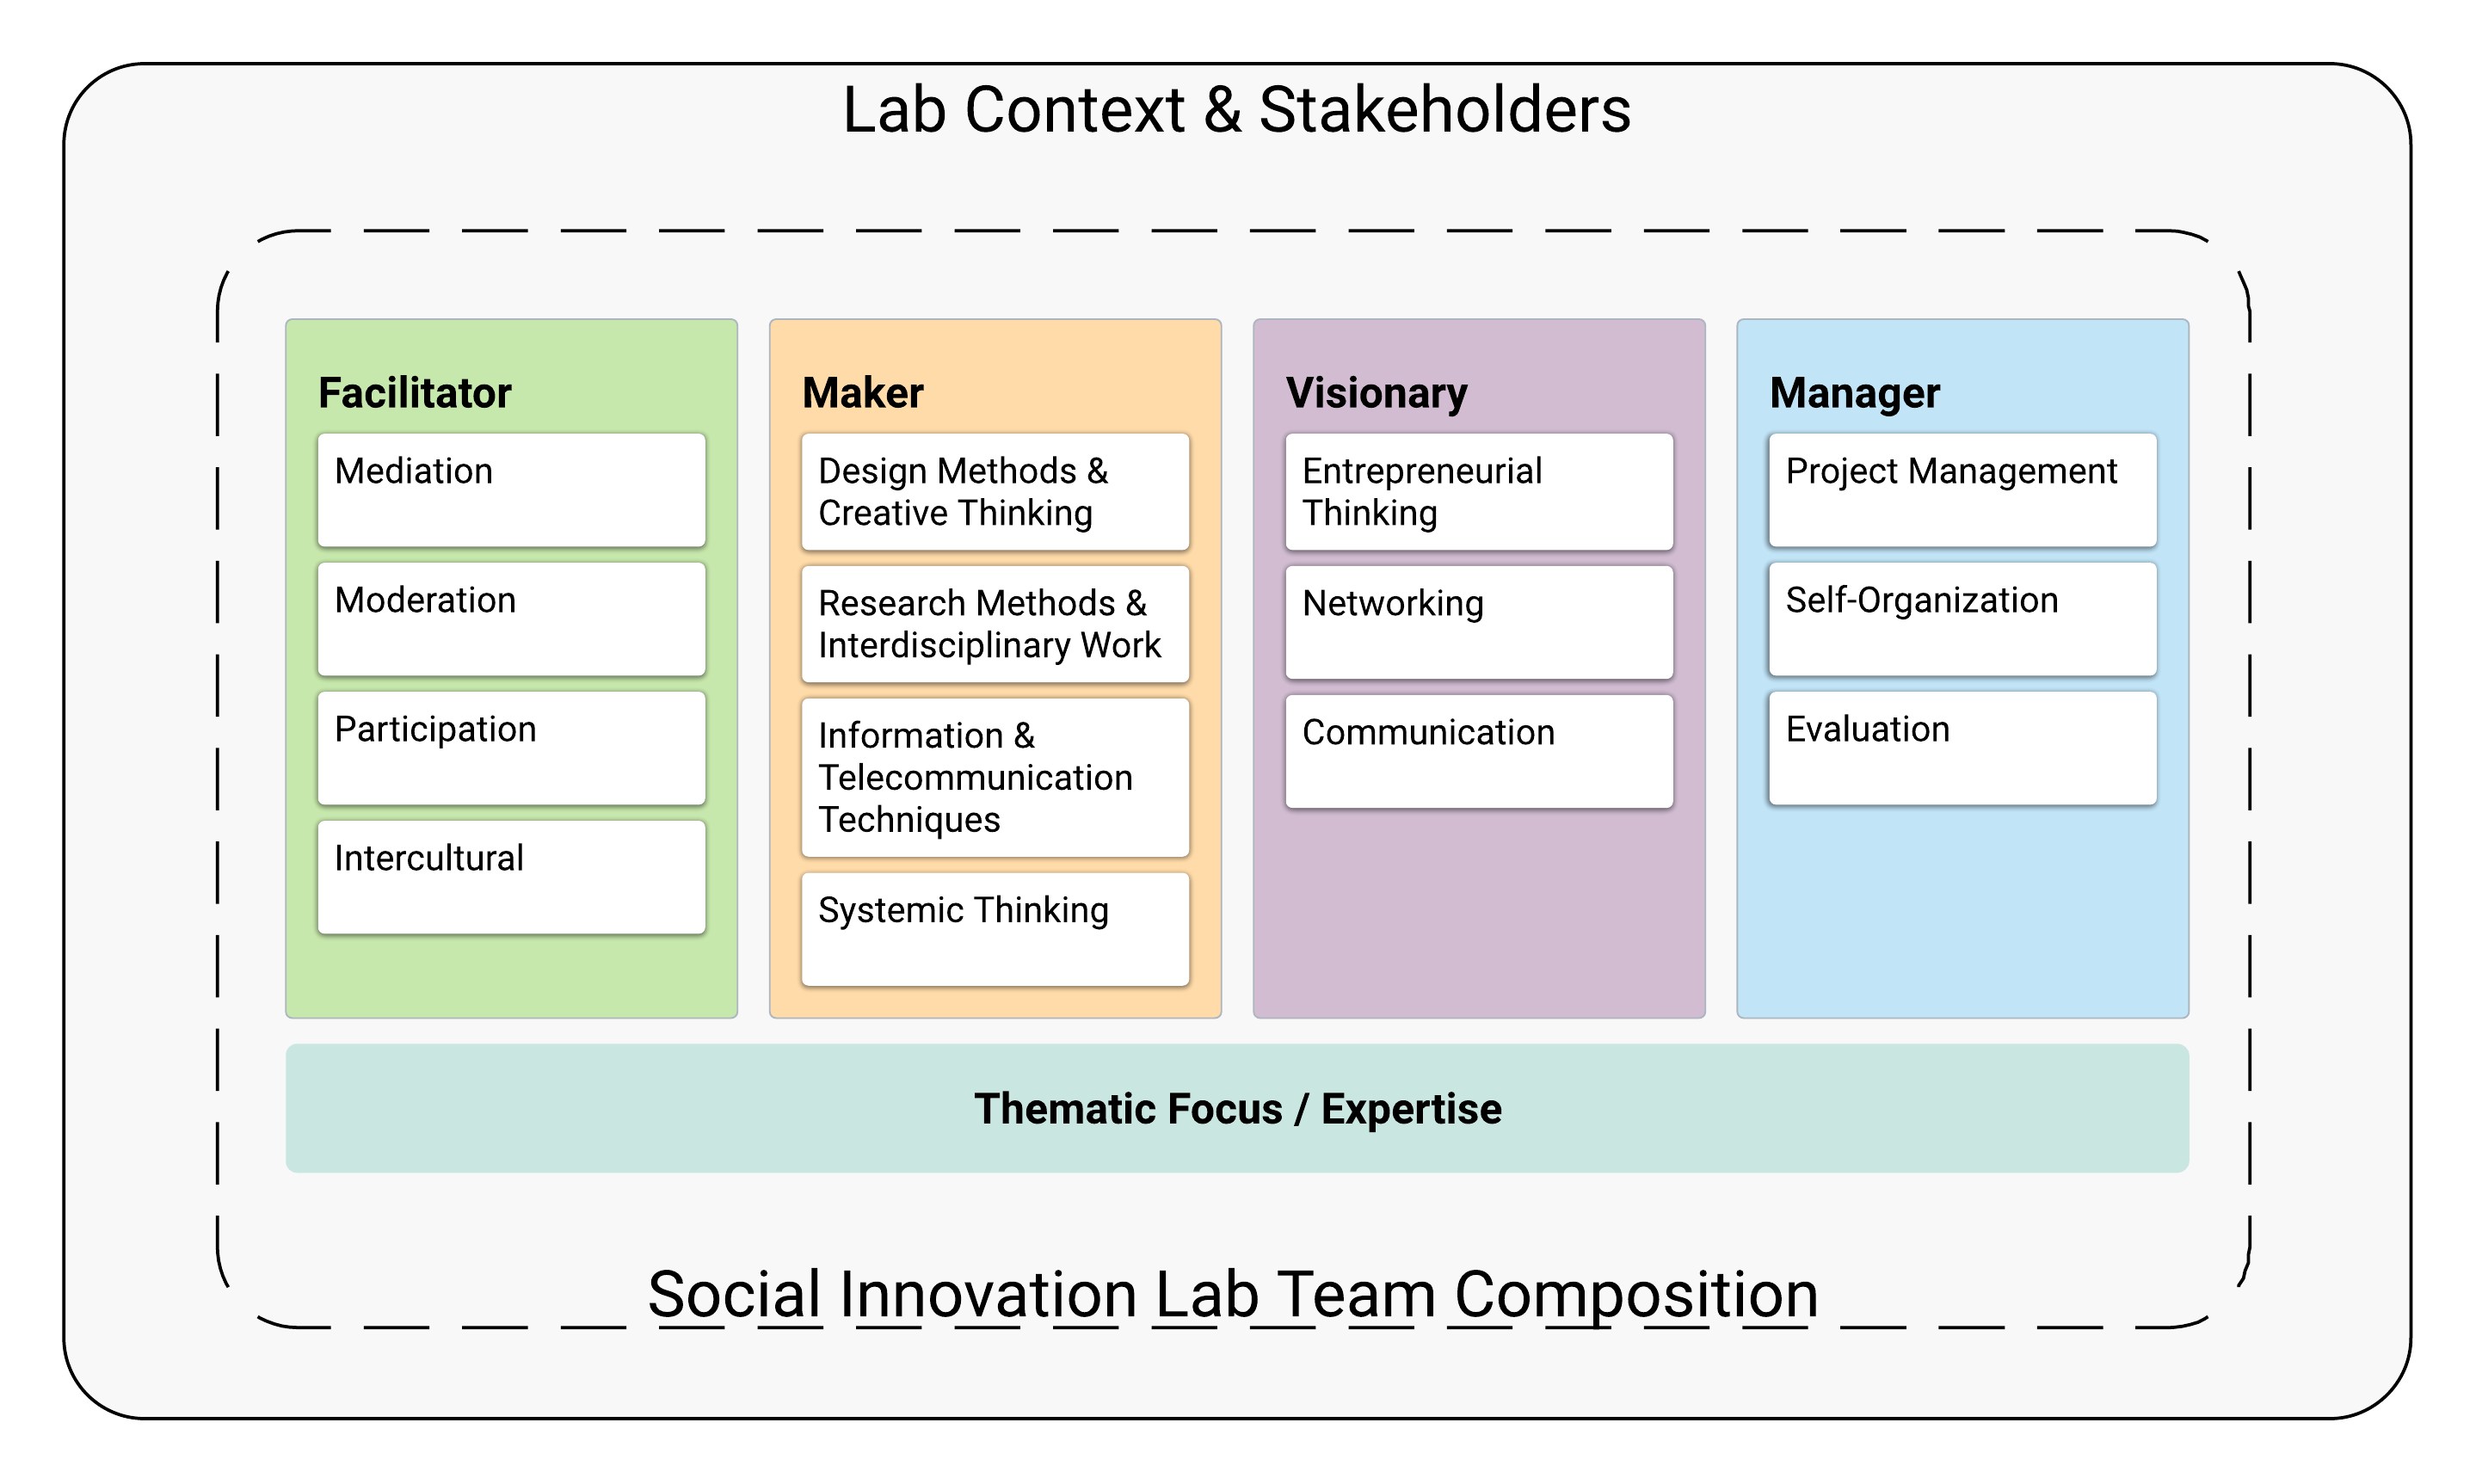
\includegraphics[width=0.95\linewidth]{Figures/Figure 2 - Role Framework} 

}

\caption{Competence-based role model proposition}\label{fig:fig2}
\end{figure}

\hypertarget{facilitators-they-who-set-the-tempo-and-orchestrate-peoples-collaboration}{%
\subsection{Facilitators -- They who set the tempo and orchestrate
people's
collaboration}\label{facilitators-they-who-set-the-tempo-and-orchestrate-peoples-collaboration}}

This is probably the most distinctive role in an innovation lab team.
The Facilitators are those who set the methodological tempo of the
projects within the lab. They know exactly what strategy, tool or
dynamics to use when divergence, convergence or a ``simple''
retrospective is needed. They get people involved and seek collaboration
for every activity. When intentions and interests collide, facilitators
keep everyone focused on the greater purpose. No collaboration is
possible where there is discrimination and exclusion, so intercultural
and transdisciplinary inclusion is a prime directive for them. What can
be expected of facilitators in a SI lab team:

\begin{itemize}
\tightlist
\item
  Design strategies, methods, and tools for orienting the innovation
  process throughout every project
  (\protect\hyperlink{ref-Belbin2010}{Belbin 2010};
  \protect\hyperlink{ref-Hering2005}{Hering and Phillips 2005};
  \protect\hyperlink{ref-Kelley2005}{Kelley and Littman 2005};
  \protect\hyperlink{ref-Gemunden2007}{Gemünden, Salomo, and Hölzle
  2007}; \protect\hyperlink{ref-Goduscheit2014}{Goduscheit 2014}).
\item
  Provide guidance and mentoring to stimulate the professional and
  personal development of project teams and participants
  (\protect\hyperlink{ref-Roberts1982}{Roberts and Fusfeld 1982};
  \protect\hyperlink{ref-Kelley2005}{Kelley and Littman 2005}).
\item
  Get people involved and encourage collaboration in every lab activity
  (\protect\hyperlink{ref-Kelley2005}{Kelley and Littman 2005};
  \protect\hyperlink{ref-Gemunden2007}{Gemünden, Salomo, and Hölzle
  2007}; \protect\hyperlink{ref-Nystrom2014}{Nyström et al. 2014};
  \protect\hyperlink{ref-Goduscheit2014}{Goduscheit 2014}).
\item
  Act as peacekeepers when a conflict emerges, maintaining the focus on
  project objectives and common goals
  (\protect\hyperlink{ref-Belbin2010}{Belbin 2010};
  \protect\hyperlink{ref-Hering2005}{Hering and Phillips 2005};
  \protect\hyperlink{ref-Nystrom2014}{Nyström et al. 2014}).
\item
  Ensure intercultural inclusiveness in all lab projects or activities
  (\protect\hyperlink{ref-Kelley2005}{Kelley and Littman 2005};
  \protect\hyperlink{ref-Nystrom2014}{Nyström et al. 2014};
  \protect\hyperlink{ref-Wascher2018}{Wascher et al. 2018}).
\end{itemize}

\hypertarget{makers-they-who-make-things-happen}{%
\subsection{Makers -- They who make things
happen}\label{makers-they-who-make-things-happen}}

Whoever comes up with an idea usually needs support to make it become
real. Makers leverage a diverse set of instrumental skills to understand
every need and to prototype any solution. They do not hesitate to mix
disciplines or to go out in the field in order to understand a problem.
They shine at combining ideas and driving innovative concepts. Makers
are driven by experimentation, iterating through prototypes crafted on
available technologies. Acknowledging the complexity of every problem in
a systemic manner is part of the way they see the world. What can be
expected of makers in a SI lab team:

\begin{itemize}
\tightlist
\item
  Understand needs and problems through the combination of multiple
  research methods and settings
  (\protect\hyperlink{ref-Kelley2005}{Kelley and Littman 2005};
  \protect\hyperlink{ref-Nystrom2014}{Nyström et al. 2014};
  \protect\hyperlink{ref-Wascher2018}{Wascher et al. 2018}).
\item
  Capture ideas, data, and any form of knowledge, restructure them and
  propose novel concept solutions
  (\protect\hyperlink{ref-Roberts1982}{Roberts and Fusfeld 1982};
  \protect\hyperlink{ref-Belbin2010}{Belbin 2010};
  \protect\hyperlink{ref-Hering2005}{Hering and Phillips 2005}).
\item
  Help build physical (and digital) representations of solutions on an
  iterative basis (\protect\hyperlink{ref-Belbin2010}{Belbin 2010};
  \protect\hyperlink{ref-Hering2005}{Hering and Phillips 2005};
  \protect\hyperlink{ref-Kelley2005}{Kelley and Littman 2005};
  \protect\hyperlink{ref-Gemunden2007}{Gemünden, Salomo, and Hölzle
  2007}; \protect\hyperlink{ref-Nystrom2014}{Nyström et al. 2014};
  \protect\hyperlink{ref-Goduscheit2014}{Goduscheit 2014}).
\item
  Propose alternatives to address the complexity of every problem and
  the systemic impact of each solution
  (\protect\hyperlink{ref-Nystrom2014}{Nyström et al. 2014};
  \protect\hyperlink{ref-Wascher2018}{Wascher et al. 2018}).
\end{itemize}

\hypertarget{visionaries-they-who-push-and-connect}{%
\subsection{Visionaries -- They who push and
connect}\label{visionaries-they-who-push-and-connect}}

Refers to the type of person who always finds an opportunity where no
one else sees it. These are the very same people who know how to easily
create networks. They possess an inherent talent for communicating their
ideas while remaining empathetic and sensitive to others. Their
particular entrepreneurial mindset keeps them moving forward, in view of
achieving their vision of the future and beliefs. What can be expected
of visionaries in a SI lab team:

\begin{itemize}
\tightlist
\item
  Provide a constant flow of ideas and project opportunities for the lab
  (\protect\hyperlink{ref-Roberts1982}{Roberts and Fusfeld 1982};
  \protect\hyperlink{ref-Hering2005}{Hering and Phillips 2005};
  \protect\hyperlink{ref-Nystrom2014}{Nyström et al. 2014}).
\item
  Build connections with communities and stakeholders to establish
  strong links between the lab, its stakeholders, and the territory
  (\protect\hyperlink{ref-Belbin2010}{Belbin 2010};
  \protect\hyperlink{ref-Hering2005}{Hering and Phillips 2005};
  \protect\hyperlink{ref-Kelley2005}{Kelley and Littman 2005};
  \protect\hyperlink{ref-Gemunden2007}{Gemünden, Salomo, and Hölzle
  2007}; \protect\hyperlink{ref-Nystrom2014}{Nyström et al. 2014};
  \protect\hyperlink{ref-Goduscheit2014}{Goduscheit 2014}).
\item
  Create an emotional connection with people around the lab by sharing
  compelling stories regarding each project, event, success, or failure
  (\protect\hyperlink{ref-Hering2005}{Hering and Phillips 2005};
  \protect\hyperlink{ref-Kelley2005}{Kelley and Littman 2005};
  \protect\hyperlink{ref-Nystrom2014}{Nyström et al. 2014};
  \protect\hyperlink{ref-Goduscheit2014}{Goduscheit 2014}).
\item
  Go out and find opportunities for the lab whether these are new
  alliances, funding options or showcase scenarios
  (\protect\hyperlink{ref-Belbin2010}{Belbin 2010};
  \protect\hyperlink{ref-Gemunden2007}{Gemünden, Salomo, and Hölzle
  2007}; \protect\hyperlink{ref-Goduscheit2014}{Goduscheit 2014};
  \protect\hyperlink{ref-Wascher2018}{Wascher et al. 2018}).
\end{itemize}

\hypertarget{managers-they-who-keep-everything-on-track}{%
\subsection{Managers -- They who keep everything on
track}\label{managers-they-who-keep-everything-on-track}}

Innovation lab initiatives can often be seen as fuzzy and accessory.
Managers are there to organize, give sense and value to everything that
happens in a lab. Because they are used to dealing with uncertain
conditions, lab managers are exceptionally adept at handling innovation
projects. They keep track of everything, detecting patterns of what
works and what does not. Their ability to monitor metrics and results
allows them to build bridges with their managerial counterparts from
other institutions to defend the role of the lab in their ecosystem. Lab
managers are capable of making decisions, a key asset in the highly
complex contexts in which labs normally operate. What can be expected of
managers in a SI lab team:

\begin{itemize}
\tightlist
\item
  Handle any technical, financial, and legal issues pertaining to the
  lab and its projects (\protect\hyperlink{ref-Gemunden2007}{Gemünden,
  Salomo, and Hölzle 2007}; \protect\hyperlink{ref-Nystrom2014}{Nyström
  et al. 2014}; \protect\hyperlink{ref-Goduscheit2014}{Goduscheit
  2014}).
\item
  Contribute to project planning while maintaining a balance between
  visionary solutions and achievable goals
  (\protect\hyperlink{ref-Roberts1982}{Roberts and Fusfeld 1982};
  \protect\hyperlink{ref-Belbin2010}{Belbin 2010};
  \protect\hyperlink{ref-Kelley2005}{Kelley and Littman 2005};
  \protect\hyperlink{ref-Nystrom2014}{Nyström et al. 2014}).
\item
  Implement monitoring and assessment mechanisms to track the lab's
  evolution and communicate results
  (\protect\hyperlink{ref-Roberts1982}{Roberts and Fusfeld 1982};
  \protect\hyperlink{ref-Belbin2010}{Belbin 2010};
  \protect\hyperlink{ref-Hering2005}{Hering and Phillips 2005}).
\item
  Have strong belief in themselves which helps them make decisions for
  the sustainability of the lab and its ecosystem
  (\protect\hyperlink{ref-Belbin2010}{Belbin 2010};
  \protect\hyperlink{ref-Gemunden2007}{Gemünden, Salomo, and Hölzle
  2007}; \protect\hyperlink{ref-Wascher2018}{Wascher et al. 2018}).
\end{itemize}

\hypertarget{tool-design-a-self-assessment-approach}{%
\subsection{Tool design: A self-assessment
approach}\label{tool-design-a-self-assessment-approach}}

The next step was to operationalize the proposed role model. Rather than
relying entirely on a rationalistic approach where functional roles are
predefined and team members are expected to fit into the assumptions, we
sought to provide a reflection and awareness tool for lab teams as they
design and implement their SI lab
(\protect\hyperlink{ref-Sandberg2000}{Sandberg 2000}). In this sense, a
self-assessment approach is instrumental in understanding the degree to
which a person considers they are competent for a determined task or in
a specific situation, while reflection processes are sparked
(\protect\hyperlink{ref-Sandberg2000}{Sandberg 2000};
\protect\hyperlink{ref-Allen2005}{Allen and Velden 2005}). An important
advantage of following a self-assessment approach is that individuals
have access to information about themselves that might otherwise be more
difficult to access (\protect\hyperlink{ref-Allen2005}{Allen and Velden
2005}). However, it is also important to be aware that relying on
self-knowledge often leads to problems regarding the reliability and
validity of results (\protect\hyperlink{ref-Ward2002}{Ward, Gruppen, and
Regehr 2002}).

For this reason, the operationalization of our theoretical model first
and foremost included the definition of short descriptions for each
competence (see Appendix A), which constitute the basis of an online
questionnaire as the first step to self-assessment. Accordingly, out of
a total of 30 questions in the online questionnaire, 23 questions are
directly related to the model criteria, 6 general questions are used for
profiling purposes and the last question is an open one to collect
feedback. Furthermore, and based on this structure, the questionnaire
was also made available in three languages: Spanish, Portuguese and
English. In terms of self-assessment levels, a scale from 0 to 5 with
anchoring phrases was applied (see Table 5). In this scale, 1
corresponds to the level where respondents understand what the
competence is but do not practice it, and 5, where they believe they
have mastered the competence and are capable of developing new ways of
applying it (\protect\hyperlink{ref-Dreyfus1986}{Dreyfus and Dreyfus
1986}). The 0 level was introduced for people who were not aware of, or
did not understand what the competence was about, so as to reduce
unintentional measurement errors
(\protect\hyperlink{ref-Allen2005}{Allen and Velden 2005}). In order to
address any ambiguity or lack of clarity, a test was performed with
several members of the consortium, prior to applying the study to the
Latin American teams. Adjustments were then made based on the feedback
and test results. The English version of the final questionnaire can be
accessed at \url{https://forms.gle/iZ1Lwyt1KUqrerb57}.

\providecommand{\docline}[3]{\noalign{\global\setlength{\arrayrulewidth}{#1}}\arrayrulecolor[HTML]{#2}\cline{#3}}

\setlength{\tabcolsep}{2pt}

\renewcommand*{\arraystretch}{1.5}

\begin{longtable}[c]{|p{1.50in}|p{1.00in}|p{2.00in}}

\caption{Self-assessment scale
}\\

\hhline{~~~}

\multicolumn{1}{!{\color[HTML]{000000}\vrule width 0pt}>{\cellcolor[HTML]{CFCFCF}\raggedright}p{\dimexpr 1.5in+0\tabcolsep+0\arrayrulewidth}}{\fontsize{8}{8}\selectfont{\textcolor[HTML]{000000}{\textbf{Level}}}} & \multicolumn{1}{!{\color[HTML]{000000}\vrule width 0pt}>{\cellcolor[HTML]{CFCFCF}\raggedleft}p{\dimexpr 1in+0\tabcolsep+0\arrayrulewidth}}{\fontsize{8}{8}\selectfont{\textcolor[HTML]{000000}{\textbf{Numeric\ Scale}}}} & \multicolumn{1}{!{\color[HTML]{000000}\vrule width 0pt}>{\cellcolor[HTML]{CFCFCF}\raggedright}p{\dimexpr 2in+0\tabcolsep+0\arrayrulewidth}!{\color[HTML]{000000}\vrule width 0pt}}{\fontsize{8}{8}\selectfont{\textcolor[HTML]{000000}{\textbf{Anchoring\ Phrases}}}} \\



\endfirsthead

\hhline{~~~}

\multicolumn{1}{!{\color[HTML]{000000}\vrule width 0pt}>{\cellcolor[HTML]{CFCFCF}\raggedright}p{\dimexpr 1.5in+0\tabcolsep+0\arrayrulewidth}}{\fontsize{8}{8}\selectfont{\textcolor[HTML]{000000}{\textbf{Level}}}} & \multicolumn{1}{!{\color[HTML]{000000}\vrule width 0pt}>{\cellcolor[HTML]{CFCFCF}\raggedleft}p{\dimexpr 1in+0\tabcolsep+0\arrayrulewidth}}{\fontsize{8}{8}\selectfont{\textcolor[HTML]{000000}{\textbf{Numeric\ Scale}}}} & \multicolumn{1}{!{\color[HTML]{000000}\vrule width 0pt}>{\cellcolor[HTML]{CFCFCF}\raggedright}p{\dimexpr 2in+0\tabcolsep+0\arrayrulewidth}!{\color[HTML]{000000}\vrule width 0pt}}{\fontsize{8}{8}\selectfont{\textcolor[HTML]{000000}{\textbf{Anchoring\ Phrases}}}} \\

\endhead



\multicolumn{1}{!{\color[HTML]{000000}\vrule width 0pt}>{\cellcolor[HTML]{EFEFEF}\raggedright}p{\dimexpr 1.5in+0\tabcolsep+0\arrayrulewidth}}{\fontsize{8}{8}\selectfont{\textcolor[HTML]{000000}{Do\ not\ understand\ /\ Not\ applicable}}} & \multicolumn{1}{!{\color[HTML]{000000}\vrule width 0pt}>{\cellcolor[HTML]{EFEFEF}\raggedleft}p{\dimexpr 1in+0\tabcolsep+0\arrayrulewidth}}{\fontsize{8}{8}\selectfont{\textcolor[HTML]{000000}{0}}} & \multicolumn{1}{!{\color[HTML]{000000}\vrule width 0pt}>{\cellcolor[HTML]{EFEFEF}\raggedright}p{\dimexpr 2in+0\tabcolsep+0\arrayrulewidth}!{\color[HTML]{000000}\vrule width 0pt}}{\fontsize{8}{8}\selectfont{\textcolor[HTML]{000000}{I\ do\ not\ understand\ what\ the\ competence\ is\ about}}} \\





\multicolumn{1}{!{\color[HTML]{000000}\vrule width 0pt}>{\raggedright}p{\dimexpr 1.5in+0\tabcolsep+0\arrayrulewidth}}{\fontsize{8}{8}\selectfont{\textcolor[HTML]{000000}{Novice}}} & \multicolumn{1}{!{\color[HTML]{000000}\vrule width 0pt}>{\raggedleft}p{\dimexpr 1in+0\tabcolsep+0\arrayrulewidth}}{\fontsize{8}{8}\selectfont{\textcolor[HTML]{000000}{1}}} & \multicolumn{1}{!{\color[HTML]{000000}\vrule width 0pt}>{\raggedright}p{\dimexpr 2in+0\tabcolsep+0\arrayrulewidth}!{\color[HTML]{000000}\vrule width 0pt}}{\fontsize{8}{8}\selectfont{\textcolor[HTML]{000000}{I\ understand\ what\ the\ competence\ is\ and\ why\ it\ is\ important\ but\ I\ don't\ use\ it}}} \\





\multicolumn{1}{!{\color[HTML]{000000}\vrule width 0pt}>{\cellcolor[HTML]{EFEFEF}\raggedright}p{\dimexpr 1.5in+0\tabcolsep+0\arrayrulewidth}}{\fontsize{8}{8}\selectfont{\textcolor[HTML]{000000}{Advanced\ beginner}}} & \multicolumn{1}{!{\color[HTML]{000000}\vrule width 0pt}>{\cellcolor[HTML]{EFEFEF}\raggedleft}p{\dimexpr 1in+0\tabcolsep+0\arrayrulewidth}}{\fontsize{8}{8}\selectfont{\textcolor[HTML]{000000}{2}}} & \multicolumn{1}{!{\color[HTML]{000000}\vrule width 0pt}>{\cellcolor[HTML]{EFEFEF}\raggedright}p{\dimexpr 2in+0\tabcolsep+0\arrayrulewidth}!{\color[HTML]{000000}\vrule width 0pt}}{\fontsize{8}{8}\selectfont{\textcolor[HTML]{000000}{I\ use\ this\ competence\ under\ supervision\ or\ with\ encouragement}}} \\





\multicolumn{1}{!{\color[HTML]{000000}\vrule width 0pt}>{\raggedright}p{\dimexpr 1.5in+0\tabcolsep+0\arrayrulewidth}}{\fontsize{8}{8}\selectfont{\textcolor[HTML]{000000}{Competent}}} & \multicolumn{1}{!{\color[HTML]{000000}\vrule width 0pt}>{\raggedleft}p{\dimexpr 1in+0\tabcolsep+0\arrayrulewidth}}{\fontsize{8}{8}\selectfont{\textcolor[HTML]{000000}{3}}} & \multicolumn{1}{!{\color[HTML]{000000}\vrule width 0pt}>{\raggedright}p{\dimexpr 2in+0\tabcolsep+0\arrayrulewidth}!{\color[HTML]{000000}\vrule width 0pt}}{\fontsize{8}{8}\selectfont{\textcolor[HTML]{000000}{I\ use\ this\ competence\ without\ supervision\ or\ encouragement}}} \\





\multicolumn{1}{!{\color[HTML]{000000}\vrule width 0pt}>{\cellcolor[HTML]{EFEFEF}\raggedright}p{\dimexpr 1.5in+0\tabcolsep+0\arrayrulewidth}}{\fontsize{8}{8}\selectfont{\textcolor[HTML]{000000}{Proficient}}} & \multicolumn{1}{!{\color[HTML]{000000}\vrule width 0pt}>{\cellcolor[HTML]{EFEFEF}\raggedleft}p{\dimexpr 1in+0\tabcolsep+0\arrayrulewidth}}{\fontsize{8}{8}\selectfont{\textcolor[HTML]{000000}{4}}} & \multicolumn{1}{!{\color[HTML]{000000}\vrule width 0pt}>{\cellcolor[HTML]{EFEFEF}\raggedright}p{\dimexpr 2in+0\tabcolsep+0\arrayrulewidth}!{\color[HTML]{000000}\vrule width 0pt}}{\fontsize{8}{8}\selectfont{\textcolor[HTML]{000000}{I\ encourage\ or\ supervise\ others\ in\ this\ competence}}} \\





\multicolumn{1}{!{\color[HTML]{000000}\vrule width 0pt}>{\raggedright}p{\dimexpr 1.5in+0\tabcolsep+0\arrayrulewidth}}{\fontsize{8}{8}\selectfont{\textcolor[HTML]{000000}{Expert}}} & \multicolumn{1}{!{\color[HTML]{000000}\vrule width 0pt}>{\raggedleft}p{\dimexpr 1in+0\tabcolsep+0\arrayrulewidth}}{\fontsize{8}{8}\selectfont{\textcolor[HTML]{000000}{5}}} & \multicolumn{1}{!{\color[HTML]{000000}\vrule width 0pt}>{\raggedright}p{\dimexpr 2in+0\tabcolsep+0\arrayrulewidth}!{\color[HTML]{000000}\vrule width 0pt}}{\fontsize{8}{8}\selectfont{\textcolor[HTML]{000000}{I\ develop\ new\ ways\ to\ apply\ this\ competence\ within\ or\ outside\ my\ organization}}} \\





\end{longtable}

Then, we designed a retrospective workshop in the form of a post
self-assessment intervention, where we asked participants to reflect on
the results of the questionnaire as a team. One of the main hypotheses
posits that a competence profile resulting from self-assessment triggers
discussion among lab team members concerning: a) the strengths and
weaknesses they may have as a team; b) the potential role(s) that each
member could play in the lab; c) the aspects to be developed and
possible strategies for doing so. In this way, lab teams are stimulated
to reflect on the current conception they have of their lab and on what
needs to be strengthened (\protect\hyperlink{ref-Sandberg2000}{Sandberg
2000}).

\hypertarget{applying-the-self-assessment-approach}{%
\section{Applying the self-assessment
approach}\label{applying-the-self-assessment-approach}}

\hypertarget{sample-and-data-collection}{%
\subsection{Sample and data
collection}\label{sample-and-data-collection}}

As previously mentioned, this study is conducted as part of the Climate
Labs project, an Erasmus+ initiative which aims to strengthen the
applied research and innovation capacities of a group of Latin American
universities, via the implementation of SI labs for mitigation and
adaptation to Climate Change. One of the project's main goals is to
build multidisciplinary teams within universities in charge of designing
a Climate Lab. Therefore, the self-assessment tool was conceived as a
starting point to this project. The methodology was applied in 10 Latin
American universities from Colombia (5), Mexico (2) and Brazil (3),
between the months of April and August 2020.

The members of each team were asked to self-assess their SI lab
competences individually by means of the online questionnaire, during
the months of April and May. Later in June, a webinar was held with all
the teams in order to share the preliminary results and introduce the
retrospective activity as the second part of the methodology. Each
university team was handed a customized report consisting mainly of
their competence profile according to our four generic role
propositions: Visionary, Maker, Facilitator and Manager. The intention
was to trigger a reflection process to identify strengths and points of
improvement and discuss them with the team. Based on the results, lab
members were also asked to state which of the proposed roles they
identified with the most and the least. Finally, they were requested to
ideate potential strategies for filling their gaps as a lab team.

A total of 65 participants completed both the questionnaire and the
workshop. Lab team size oscillated between 4 and 13 members. Among the
respondents there were faculty members, administration staff,
researchers and students, the latter category being only represented by
three undergraduate students and one doctoral student. This was mainly
due to the constraints of the global COVID-19 health crisis, with
repercussions on each university's academic schedule. Nevertheless, the
sample is still representative of who will lead lab implementation,
which guarantees that insights drawn from this analysis will provide a
real picture of a SI lab team in its early stages. Table 6 summarizes
team composition by university.

\providecommand{\docline}[3]{\noalign{\global\setlength{\arrayrulewidth}{#1}}\arrayrulecolor[HTML]{#2}\cline{#3}}

\setlength{\tabcolsep}{2pt}

\renewcommand*{\arraystretch}{1.5}

\begin{longtable}[c]{|p{0.80in}|p{0.40in}|p{0.30in}|p{0.30in}|p{0.30in}|p{0.30in}|p{0.30in}|p{0.30in}|p{0.30in}|p{0.50in}|p{2.00in}}

\caption{Lab team composition and thematic focus
}\\

\hhline{>{\arrayrulecolor[HTML]{666666}\global\arrayrulewidth=2pt}->{\arrayrulecolor[HTML]{666666}\global\arrayrulewidth=2pt}->{\arrayrulecolor[HTML]{666666}\global\arrayrulewidth=2pt}->{\arrayrulecolor[HTML]{666666}\global\arrayrulewidth=2pt}->{\arrayrulecolor[HTML]{666666}\global\arrayrulewidth=2pt}->{\arrayrulecolor[HTML]{666666}\global\arrayrulewidth=2pt}->{\arrayrulecolor[HTML]{666666}\global\arrayrulewidth=2pt}->{\arrayrulecolor[HTML]{666666}\global\arrayrulewidth=2pt}->{\arrayrulecolor[HTML]{666666}\global\arrayrulewidth=2pt}->{\arrayrulecolor[HTML]{666666}\global\arrayrulewidth=2pt}->{\arrayrulecolor[HTML]{666666}\global\arrayrulewidth=2pt}-}

\multicolumn{2}{!{\color[HTML]{000000}\vrule width 0pt}>{\raggedright}p{\dimexpr 1.2in+2\tabcolsep+1\arrayrulewidth}}{\fontsize{8}{8}\selectfont{\textcolor[HTML]{000000}{}}} & \multicolumn{7}{!{\color[HTML]{E3E3E3}\vrule width 0.1pt}>{\raggedright}p{\dimexpr 2.1in+12\tabcolsep+6\arrayrulewidth}}{\fontsize{8}{8}\selectfont{\textcolor[HTML]{000000}{Members\ by\ Position}}} & \multicolumn{2}{!{\color[HTML]{E3E3E3}\vrule width 0.1pt}>{\raggedright}p{\dimexpr 2.5in+2\tabcolsep+1\arrayrulewidth}!{\color[HTML]{E3E3E3}\vrule width 0.1pt}}{\fontsize{8}{8}\selectfont{\textcolor[HTML]{000000}{}}} \\

\hhline{>{\arrayrulecolor[HTML]{E3E3E3}\global\arrayrulewidth=0.1pt}->{\arrayrulecolor[HTML]{E3E3E3}\global\arrayrulewidth=0.1pt}->{\arrayrulecolor[HTML]{E3E3E3}\global\arrayrulewidth=0.1pt}->{\arrayrulecolor[HTML]{E3E3E3}\global\arrayrulewidth=0.1pt}->{\arrayrulecolor[HTML]{E3E3E3}\global\arrayrulewidth=0.1pt}->{\arrayrulecolor[HTML]{E3E3E3}\global\arrayrulewidth=0.1pt}->{\arrayrulecolor[HTML]{E3E3E3}\global\arrayrulewidth=0.1pt}->{\arrayrulecolor[HTML]{E3E3E3}\global\arrayrulewidth=0.1pt}->{\arrayrulecolor[HTML]{E3E3E3}\global\arrayrulewidth=0.1pt}->{\arrayrulecolor[HTML]{E3E3E3}\global\arrayrulewidth=0.1pt}->{\arrayrulecolor[HTML]{E3E3E3}\global\arrayrulewidth=0.1pt}-}

\multicolumn{1}{!{\color[HTML]{000000}\vrule width 0pt}>{\raggedright}p{\dimexpr 0.8in+0\tabcolsep+0\arrayrulewidth}}{\fontsize{8}{8}\selectfont{\textcolor[HTML]{000000}{Country}}} & \multicolumn{1}{!{\color[HTML]{E3E3E3}\vrule width 0.1pt}>{\raggedright}p{\dimexpr 0.4in+0\tabcolsep+0\arrayrulewidth}}{\fontsize{8}{8}\selectfont{\textcolor[HTML]{000000}{SI\ Lab}}} & \multicolumn{1}{!{\color[HTML]{E3E3E3}\vrule width 0.1pt}>{\raggedright}p{\dimexpr 0.3in+0\tabcolsep+0\arrayrulewidth}}{\fontsize{8}{8}\selectfont{\textcolor[HTML]{000000}{PR}}\fontsize{8}{8}\selectfont{\textsuperscript{\textcolor[HTML]{000000}{}}}} & \multicolumn{1}{!{\color[HTML]{E3E3E3}\vrule width 0.1pt}>{\raggedright}p{\dimexpr 0.3in+0\tabcolsep+0\arrayrulewidth}}{\fontsize{8}{8}\selectfont{\textcolor[HTML]{000000}{AP}}\fontsize{8}{8}\selectfont{\textsuperscript{\textcolor[HTML]{000000}{}}}} & \multicolumn{1}{!{\color[HTML]{E3E3E3}\vrule width 0.1pt}>{\raggedright}p{\dimexpr 0.3in+0\tabcolsep+0\arrayrulewidth}}{\fontsize{8}{8}\selectfont{\textcolor[HTML]{000000}{DI}}\fontsize{8}{8}\selectfont{\textsuperscript{\textcolor[HTML]{000000}{}}}} & \multicolumn{1}{!{\color[HTML]{E3E3E3}\vrule width 0.1pt}>{\raggedright}p{\dimexpr 0.3in+0\tabcolsep+0\arrayrulewidth}}{\fontsize{8}{8}\selectfont{\textcolor[HTML]{000000}{AS}}\fontsize{8}{8}\selectfont{\textsuperscript{\textcolor[HTML]{000000}{}}}} & \multicolumn{1}{!{\color[HTML]{E3E3E3}\vrule width 0.1pt}>{\raggedright}p{\dimexpr 0.3in+0\tabcolsep+0\arrayrulewidth}}{\fontsize{8}{8}\selectfont{\textcolor[HTML]{000000}{ST}}\fontsize{8}{8}\selectfont{\textsuperscript{\textcolor[HTML]{000000}{}}}} & \multicolumn{1}{!{\color[HTML]{E3E3E3}\vrule width 0.1pt}>{\raggedright}p{\dimexpr 0.3in+0\tabcolsep+0\arrayrulewidth}}{\fontsize{8}{8}\selectfont{\textcolor[HTML]{000000}{RE}}\fontsize{8}{8}\selectfont{\textsuperscript{\textcolor[HTML]{000000}{}}}} & \multicolumn{1}{!{\color[HTML]{E3E3E3}\vrule width 0.1pt}>{\raggedright}p{\dimexpr 0.3in+0\tabcolsep+0\arrayrulewidth}}{\fontsize{8}{8}\selectfont{\textcolor[HTML]{000000}{OT}}\fontsize{8}{8}\selectfont{\textsuperscript{\textcolor[HTML]{000000}{}}}} & \multicolumn{1}{!{\color[HTML]{E3E3E3}\vrule width 0.1pt}>{\raggedright}p{\dimexpr 0.5in+0\tabcolsep+0\arrayrulewidth}}{\fontsize{8}{8}\selectfont{\textcolor[HTML]{000000}{Lab\ Team\ Size}}} & \multicolumn{1}{!{\color[HTML]{E3E3E3}\vrule width 0.1pt}>{\raggedright}p{\dimexpr 2in+0\tabcolsep+0\arrayrulewidth}!{\color[HTML]{000000}\vrule width 0pt}}{\fontsize{8}{8}\selectfont{\textcolor[HTML]{000000}{Thematic\ Focus}}} \\

\hhline{>{\arrayrulecolor[HTML]{666666}\global\arrayrulewidth=2pt}->{\arrayrulecolor[HTML]{666666}\global\arrayrulewidth=2pt}->{\arrayrulecolor[HTML]{666666}\global\arrayrulewidth=2pt}->{\arrayrulecolor[HTML]{666666}\global\arrayrulewidth=2pt}->{\arrayrulecolor[HTML]{666666}\global\arrayrulewidth=2pt}->{\arrayrulecolor[HTML]{666666}\global\arrayrulewidth=2pt}->{\arrayrulecolor[HTML]{666666}\global\arrayrulewidth=2pt}->{\arrayrulecolor[HTML]{666666}\global\arrayrulewidth=2pt}->{\arrayrulecolor[HTML]{666666}\global\arrayrulewidth=2pt}->{\arrayrulecolor[HTML]{666666}\global\arrayrulewidth=2pt}->{\arrayrulecolor[HTML]{666666}\global\arrayrulewidth=2pt}-}

\endfirsthead

\hhline{>{\arrayrulecolor[HTML]{666666}\global\arrayrulewidth=2pt}->{\arrayrulecolor[HTML]{666666}\global\arrayrulewidth=2pt}->{\arrayrulecolor[HTML]{666666}\global\arrayrulewidth=2pt}->{\arrayrulecolor[HTML]{666666}\global\arrayrulewidth=2pt}->{\arrayrulecolor[HTML]{666666}\global\arrayrulewidth=2pt}->{\arrayrulecolor[HTML]{666666}\global\arrayrulewidth=2pt}->{\arrayrulecolor[HTML]{666666}\global\arrayrulewidth=2pt}->{\arrayrulecolor[HTML]{666666}\global\arrayrulewidth=2pt}->{\arrayrulecolor[HTML]{666666}\global\arrayrulewidth=2pt}->{\arrayrulecolor[HTML]{666666}\global\arrayrulewidth=2pt}->{\arrayrulecolor[HTML]{666666}\global\arrayrulewidth=2pt}-}

\multicolumn{2}{!{\color[HTML]{000000}\vrule width 0pt}>{\raggedright}p{\dimexpr 1.2in+2\tabcolsep+1\arrayrulewidth}}{\fontsize{8}{8}\selectfont{\textcolor[HTML]{000000}{}}} & \multicolumn{7}{!{\color[HTML]{E3E3E3}\vrule width 0.1pt}>{\raggedright}p{\dimexpr 2.1in+12\tabcolsep+6\arrayrulewidth}}{\fontsize{8}{8}\selectfont{\textcolor[HTML]{000000}{Members\ by\ Position}}} & \multicolumn{2}{!{\color[HTML]{E3E3E3}\vrule width 0.1pt}>{\raggedright}p{\dimexpr 2.5in+2\tabcolsep+1\arrayrulewidth}!{\color[HTML]{E3E3E3}\vrule width 0.1pt}}{\fontsize{8}{8}\selectfont{\textcolor[HTML]{000000}{}}} \\

\hhline{>{\arrayrulecolor[HTML]{E3E3E3}\global\arrayrulewidth=0.1pt}->{\arrayrulecolor[HTML]{E3E3E3}\global\arrayrulewidth=0.1pt}->{\arrayrulecolor[HTML]{E3E3E3}\global\arrayrulewidth=0.1pt}->{\arrayrulecolor[HTML]{E3E3E3}\global\arrayrulewidth=0.1pt}->{\arrayrulecolor[HTML]{E3E3E3}\global\arrayrulewidth=0.1pt}->{\arrayrulecolor[HTML]{E3E3E3}\global\arrayrulewidth=0.1pt}->{\arrayrulecolor[HTML]{E3E3E3}\global\arrayrulewidth=0.1pt}->{\arrayrulecolor[HTML]{E3E3E3}\global\arrayrulewidth=0.1pt}->{\arrayrulecolor[HTML]{E3E3E3}\global\arrayrulewidth=0.1pt}->{\arrayrulecolor[HTML]{E3E3E3}\global\arrayrulewidth=0.1pt}->{\arrayrulecolor[HTML]{E3E3E3}\global\arrayrulewidth=0.1pt}-}



\multicolumn{1}{!{\color[HTML]{000000}\vrule width 0pt}>{\raggedright}p{\dimexpr 0.8in+0\tabcolsep+0\arrayrulewidth}}{\fontsize{8}{8}\selectfont{\textcolor[HTML]{000000}{Country}}} & \multicolumn{1}{!{\color[HTML]{E3E3E3}\vrule width 0.1pt}>{\raggedright}p{\dimexpr 0.4in+0\tabcolsep+0\arrayrulewidth}}{\fontsize{8}{8}\selectfont{\textcolor[HTML]{000000}{SI\ Lab}}} & \multicolumn{1}{!{\color[HTML]{E3E3E3}\vrule width 0.1pt}>{\raggedright}p{\dimexpr 0.3in+0\tabcolsep+0\arrayrulewidth}}{\fontsize{8}{8}\selectfont{\textcolor[HTML]{000000}{PR}}\fontsize{8}{8}\selectfont{\textsuperscript{\textcolor[HTML]{000000}{}}}} & \multicolumn{1}{!{\color[HTML]{E3E3E3}\vrule width 0.1pt}>{\raggedright}p{\dimexpr 0.3in+0\tabcolsep+0\arrayrulewidth}}{\fontsize{8}{8}\selectfont{\textcolor[HTML]{000000}{AP}}\fontsize{8}{8}\selectfont{\textsuperscript{\textcolor[HTML]{000000}{}}}} & \multicolumn{1}{!{\color[HTML]{E3E3E3}\vrule width 0.1pt}>{\raggedright}p{\dimexpr 0.3in+0\tabcolsep+0\arrayrulewidth}}{\fontsize{8}{8}\selectfont{\textcolor[HTML]{000000}{DI}}\fontsize{8}{8}\selectfont{\textsuperscript{\textcolor[HTML]{000000}{}}}} & \multicolumn{1}{!{\color[HTML]{E3E3E3}\vrule width 0.1pt}>{\raggedright}p{\dimexpr 0.3in+0\tabcolsep+0\arrayrulewidth}}{\fontsize{8}{8}\selectfont{\textcolor[HTML]{000000}{AS}}\fontsize{8}{8}\selectfont{\textsuperscript{\textcolor[HTML]{000000}{}}}} & \multicolumn{1}{!{\color[HTML]{E3E3E3}\vrule width 0.1pt}>{\raggedright}p{\dimexpr 0.3in+0\tabcolsep+0\arrayrulewidth}}{\fontsize{8}{8}\selectfont{\textcolor[HTML]{000000}{ST}}\fontsize{8}{8}\selectfont{\textsuperscript{\textcolor[HTML]{000000}{}}}} & \multicolumn{1}{!{\color[HTML]{E3E3E3}\vrule width 0.1pt}>{\raggedright}p{\dimexpr 0.3in+0\tabcolsep+0\arrayrulewidth}}{\fontsize{8}{8}\selectfont{\textcolor[HTML]{000000}{RE}}\fontsize{8}{8}\selectfont{\textsuperscript{\textcolor[HTML]{000000}{}}}} & \multicolumn{1}{!{\color[HTML]{E3E3E3}\vrule width 0.1pt}>{\raggedright}p{\dimexpr 0.3in+0\tabcolsep+0\arrayrulewidth}}{\fontsize{8}{8}\selectfont{\textcolor[HTML]{000000}{OT}}\fontsize{8}{8}\selectfont{\textsuperscript{\textcolor[HTML]{000000}{}}}} & \multicolumn{1}{!{\color[HTML]{E3E3E3}\vrule width 0.1pt}>{\raggedright}p{\dimexpr 0.5in+0\tabcolsep+0\arrayrulewidth}}{\fontsize{8}{8}\selectfont{\textcolor[HTML]{000000}{Lab\ Team\ Size}}} & \multicolumn{1}{!{\color[HTML]{E3E3E3}\vrule width 0.1pt}>{\raggedright}p{\dimexpr 2in+0\tabcolsep+0\arrayrulewidth}!{\color[HTML]{000000}\vrule width 0pt}}{\fontsize{8}{8}\selectfont{\textcolor[HTML]{000000}{Thematic\ Focus}}} \\

\hhline{>{\arrayrulecolor[HTML]{666666}\global\arrayrulewidth=2pt}->{\arrayrulecolor[HTML]{666666}\global\arrayrulewidth=2pt}->{\arrayrulecolor[HTML]{666666}\global\arrayrulewidth=2pt}->{\arrayrulecolor[HTML]{666666}\global\arrayrulewidth=2pt}->{\arrayrulecolor[HTML]{666666}\global\arrayrulewidth=2pt}->{\arrayrulecolor[HTML]{666666}\global\arrayrulewidth=2pt}->{\arrayrulecolor[HTML]{666666}\global\arrayrulewidth=2pt}->{\arrayrulecolor[HTML]{666666}\global\arrayrulewidth=2pt}->{\arrayrulecolor[HTML]{666666}\global\arrayrulewidth=2pt}->{\arrayrulecolor[HTML]{666666}\global\arrayrulewidth=2pt}->{\arrayrulecolor[HTML]{666666}\global\arrayrulewidth=2pt}-}\endhead



\multicolumn{11}{!{\color[HTML]{FFFFFF}\vrule width 0pt}>{\raggedright}p{\dimexpr 5.8in+20\tabcolsep+10\arrayrulewidth}!{\color[HTML]{FFFFFF}\vrule width 0pt}}{\fontsize{11}{11}\selectfont{\textsuperscript{\textcolor[HTML]{000000}{}}}\fontsize{11}{11}\selectfont{\textcolor[HTML]{000000}{PR:\ Professor}}\fontsize{11}{11}\selectfont{\textcolor[HTML]{000000}{;\ }}\fontsize{11}{11}\selectfont{\textsuperscript{\textcolor[HTML]{000000}{}}}\fontsize{11}{11}\selectfont{\textcolor[HTML]{000000}{AP:\ Assistant\ Professor}}\fontsize{11}{11}\selectfont{\textcolor[HTML]{000000}{;\ }}\fontsize{11}{11}\selectfont{\textsuperscript{\textcolor[HTML]{000000}{}}}\fontsize{11}{11}\selectfont{\textcolor[HTML]{000000}{DI:\ Director}}\fontsize{11}{11}\selectfont{\textcolor[HTML]{000000}{;\ }}\fontsize{11}{11}\selectfont{\textsuperscript{\textcolor[HTML]{000000}{}}}\fontsize{11}{11}\selectfont{\textcolor[HTML]{000000}{AS:\ Administrative\ Staff}}\fontsize{11}{11}\selectfont{\textcolor[HTML]{000000}{;\ }}\fontsize{11}{11}\selectfont{\textsuperscript{\textcolor[HTML]{000000}{}}}\fontsize{11}{11}\selectfont{\textcolor[HTML]{000000}{RE:\ Researcher}}\fontsize{11}{11}\selectfont{\textcolor[HTML]{000000}{;\ }}\fontsize{11}{11}\selectfont{\textsuperscript{\textcolor[HTML]{000000}{}}}\fontsize{11}{11}\selectfont{\textcolor[HTML]{000000}{ST:\ Student}}\fontsize{11}{11}\selectfont{\textcolor[HTML]{000000}{;\ }}\fontsize{11}{11}\selectfont{\textsuperscript{\textcolor[HTML]{000000}{}}}\fontsize{11}{11}\selectfont{\textcolor[HTML]{000000}{OT:\ Other}}} \\

\endfoot



\multicolumn{1}{!{\color[HTML]{000000}\vrule width 0pt}>{\raggedright}p{\dimexpr 0.8in+0\tabcolsep+0\arrayrulewidth}}{} & \multicolumn{1}{!{\color[HTML]{E3E3E3}\vrule width 0.1pt}>{\raggedright}p{\dimexpr 0.4in+0\tabcolsep+0\arrayrulewidth}}{\fontsize{8}{8}\selectfont{\textcolor[HTML]{000000}{A}}} & \multicolumn{1}{!{\color[HTML]{E3E3E3}\vrule width 0.1pt}>{\raggedright}p{\dimexpr 0.3in+0\tabcolsep+0\arrayrulewidth}}{\fontsize{8}{8}\selectfont{\textcolor[HTML]{000000}{5}}} & \multicolumn{1}{!{\color[HTML]{E3E3E3}\vrule width 0.1pt}>{\raggedright}p{\dimexpr 0.3in+0\tabcolsep+0\arrayrulewidth}}{\fontsize{8}{8}\selectfont{\textcolor[HTML]{000000}{2}}} & \multicolumn{1}{!{\color[HTML]{E3E3E3}\vrule width 0.1pt}>{\raggedright}p{\dimexpr 0.3in+0\tabcolsep+0\arrayrulewidth}}{\fontsize{8}{8}\selectfont{\textcolor[HTML]{000000}{2}}} & \multicolumn{1}{!{\color[HTML]{E3E3E3}\vrule width 0.1pt}>{\raggedright}p{\dimexpr 0.3in+0\tabcolsep+0\arrayrulewidth}}{\fontsize{8}{8}\selectfont{\textcolor[HTML]{000000}{1}}} & \multicolumn{1}{!{\color[HTML]{E3E3E3}\vrule width 0.1pt}>{\raggedright}p{\dimexpr 0.3in+0\tabcolsep+0\arrayrulewidth}}{\fontsize{8}{8}\selectfont{\textcolor[HTML]{000000}{1}}} & \multicolumn{1}{!{\color[HTML]{E3E3E3}\vrule width 0.1pt}>{\raggedright}p{\dimexpr 0.3in+0\tabcolsep+0\arrayrulewidth}}{\fontsize{8}{8}\selectfont{\textcolor[HTML]{000000}{2}}} & \multicolumn{1}{!{\color[HTML]{E3E3E3}\vrule width 0.1pt}>{\raggedright}p{\dimexpr 0.3in+0\tabcolsep+0\arrayrulewidth}}{\fontsize{8}{8}\selectfont{\textcolor[HTML]{000000}{-}}} & \multicolumn{1}{!{\color[HTML]{E3E3E3}\vrule width 0.1pt}>{\raggedright}p{\dimexpr 0.5in+0\tabcolsep+0\arrayrulewidth}}{\fontsize{8}{8}\selectfont{\textcolor[HTML]{000000}{13}}} & \multicolumn{1}{!{\color[HTML]{E3E3E3}\vrule width 0.1pt}>{\raggedright}p{\dimexpr 2in+0\tabcolsep+0\arrayrulewidth}!{\color[HTML]{000000}\vrule width 0pt}}{\fontsize{8}{8}\selectfont{\textcolor[HTML]{000000}{Urban\ Flood\ and\ Heat\ Island\ Management}}} \\

\hhline{~>{\arrayrulecolor[HTML]{E3E3E3}\global\arrayrulewidth=0.1pt}->{\arrayrulecolor[HTML]{E3E3E3}\global\arrayrulewidth=0.1pt}->{\arrayrulecolor[HTML]{E3E3E3}\global\arrayrulewidth=0.1pt}->{\arrayrulecolor[HTML]{E3E3E3}\global\arrayrulewidth=0.1pt}->{\arrayrulecolor[HTML]{E3E3E3}\global\arrayrulewidth=0.1pt}->{\arrayrulecolor[HTML]{E3E3E3}\global\arrayrulewidth=0.1pt}->{\arrayrulecolor[HTML]{E3E3E3}\global\arrayrulewidth=0.1pt}->{\arrayrulecolor[HTML]{E3E3E3}\global\arrayrulewidth=0.1pt}->{\arrayrulecolor[HTML]{E3E3E3}\global\arrayrulewidth=0.1pt}->{\arrayrulecolor[HTML]{E3E3E3}\global\arrayrulewidth=0.1pt}-}



\multicolumn{1}{!{\color[HTML]{000000}\vrule width 0pt}>{\raggedright}p{\dimexpr 0.8in+0\tabcolsep+0\arrayrulewidth}}{} & \multicolumn{1}{!{\color[HTML]{E3E3E3}\vrule width 0.1pt}>{\raggedright}p{\dimexpr 0.4in+0\tabcolsep+0\arrayrulewidth}}{\fontsize{8}{8}\selectfont{\textcolor[HTML]{000000}{B}}} & \multicolumn{1}{!{\color[HTML]{E3E3E3}\vrule width 0.1pt}>{\raggedright}p{\dimexpr 0.3in+0\tabcolsep+0\arrayrulewidth}}{\fontsize{8}{8}\selectfont{\textcolor[HTML]{000000}{1}}} & \multicolumn{1}{!{\color[HTML]{E3E3E3}\vrule width 0.1pt}>{\raggedright}p{\dimexpr 0.3in+0\tabcolsep+0\arrayrulewidth}}{\fontsize{8}{8}\selectfont{\textcolor[HTML]{000000}{1}}} & \multicolumn{1}{!{\color[HTML]{E3E3E3}\vrule width 0.1pt}>{\raggedright}p{\dimexpr 0.3in+0\tabcolsep+0\arrayrulewidth}}{\fontsize{8}{8}\selectfont{\textcolor[HTML]{000000}{1}}} & \multicolumn{1}{!{\color[HTML]{E3E3E3}\vrule width 0.1pt}>{\raggedright}p{\dimexpr 0.3in+0\tabcolsep+0\arrayrulewidth}}{\fontsize{8}{8}\selectfont{\textcolor[HTML]{000000}{1}}} & \multicolumn{1}{!{\color[HTML]{E3E3E3}\vrule width 0.1pt}>{\raggedright}p{\dimexpr 0.3in+0\tabcolsep+0\arrayrulewidth}}{\fontsize{8}{8}\selectfont{\textcolor[HTML]{000000}{-}}} & \multicolumn{1}{!{\color[HTML]{E3E3E3}\vrule width 0.1pt}>{\raggedright}p{\dimexpr 0.3in+0\tabcolsep+0\arrayrulewidth}}{\fontsize{8}{8}\selectfont{\textcolor[HTML]{000000}{-}}} & \multicolumn{1}{!{\color[HTML]{E3E3E3}\vrule width 0.1pt}>{\raggedright}p{\dimexpr 0.3in+0\tabcolsep+0\arrayrulewidth}}{\fontsize{8}{8}\selectfont{\textcolor[HTML]{000000}{-}}} & \multicolumn{1}{!{\color[HTML]{E3E3E3}\vrule width 0.1pt}>{\raggedright}p{\dimexpr 0.5in+0\tabcolsep+0\arrayrulewidth}}{\fontsize{8}{8}\selectfont{\textcolor[HTML]{000000}{4}}} & \multicolumn{1}{!{\color[HTML]{E3E3E3}\vrule width 0.1pt}>{\raggedright}p{\dimexpr 2in+0\tabcolsep+0\arrayrulewidth}!{\color[HTML]{000000}\vrule width 0pt}}{\fontsize{8}{8}\selectfont{\textcolor[HTML]{000000}{SI\ and\ Community\ Development}}} \\

\hhline{~>{\arrayrulecolor[HTML]{E3E3E3}\global\arrayrulewidth=0.1pt}->{\arrayrulecolor[HTML]{E3E3E3}\global\arrayrulewidth=0.1pt}->{\arrayrulecolor[HTML]{E3E3E3}\global\arrayrulewidth=0.1pt}->{\arrayrulecolor[HTML]{E3E3E3}\global\arrayrulewidth=0.1pt}->{\arrayrulecolor[HTML]{E3E3E3}\global\arrayrulewidth=0.1pt}->{\arrayrulecolor[HTML]{E3E3E3}\global\arrayrulewidth=0.1pt}->{\arrayrulecolor[HTML]{E3E3E3}\global\arrayrulewidth=0.1pt}->{\arrayrulecolor[HTML]{E3E3E3}\global\arrayrulewidth=0.1pt}->{\arrayrulecolor[HTML]{E3E3E3}\global\arrayrulewidth=0.1pt}->{\arrayrulecolor[HTML]{E3E3E3}\global\arrayrulewidth=0.1pt}-}



\multicolumn{1}{!{\color[HTML]{000000}\vrule width 0pt}>{\raggedright}p{\dimexpr 0.8in+0\tabcolsep+0\arrayrulewidth}}{\multirow[c]{-3}{*}{\fontsize{8}{8}\selectfont{\textcolor[HTML]{000000}{Brazil}}}} & \multicolumn{1}{!{\color[HTML]{E3E3E3}\vrule width 0.1pt}>{\raggedright}p{\dimexpr 0.4in+0\tabcolsep+0\arrayrulewidth}}{\fontsize{8}{8}\selectfont{\textcolor[HTML]{000000}{C}}} & \multicolumn{1}{!{\color[HTML]{E3E3E3}\vrule width 0.1pt}>{\raggedright}p{\dimexpr 0.3in+0\tabcolsep+0\arrayrulewidth}}{\fontsize{8}{8}\selectfont{\textcolor[HTML]{000000}{6}}} & \multicolumn{1}{!{\color[HTML]{E3E3E3}\vrule width 0.1pt}>{\raggedright}p{\dimexpr 0.3in+0\tabcolsep+0\arrayrulewidth}}{\fontsize{8}{8}\selectfont{\textcolor[HTML]{000000}{1}}} & \multicolumn{1}{!{\color[HTML]{E3E3E3}\vrule width 0.1pt}>{\raggedright}p{\dimexpr 0.3in+0\tabcolsep+0\arrayrulewidth}}{\fontsize{8}{8}\selectfont{\textcolor[HTML]{000000}{-}}} & \multicolumn{1}{!{\color[HTML]{E3E3E3}\vrule width 0.1pt}>{\raggedright}p{\dimexpr 0.3in+0\tabcolsep+0\arrayrulewidth}}{\fontsize{8}{8}\selectfont{\textcolor[HTML]{000000}{-}}} & \multicolumn{1}{!{\color[HTML]{E3E3E3}\vrule width 0.1pt}>{\raggedright}p{\dimexpr 0.3in+0\tabcolsep+0\arrayrulewidth}}{\fontsize{8}{8}\selectfont{\textcolor[HTML]{000000}{3}}} & \multicolumn{1}{!{\color[HTML]{E3E3E3}\vrule width 0.1pt}>{\raggedright}p{\dimexpr 0.3in+0\tabcolsep+0\arrayrulewidth}}{\fontsize{8}{8}\selectfont{\textcolor[HTML]{000000}{-}}} & \multicolumn{1}{!{\color[HTML]{E3E3E3}\vrule width 0.1pt}>{\raggedright}p{\dimexpr 0.3in+0\tabcolsep+0\arrayrulewidth}}{\fontsize{8}{8}\selectfont{\textcolor[HTML]{000000}{-}}} & \multicolumn{1}{!{\color[HTML]{E3E3E3}\vrule width 0.1pt}>{\raggedright}p{\dimexpr 0.5in+0\tabcolsep+0\arrayrulewidth}}{\fontsize{8}{8}\selectfont{\textcolor[HTML]{000000}{10}}} & \multicolumn{1}{!{\color[HTML]{E3E3E3}\vrule width 0.1pt}>{\raggedright}p{\dimexpr 2in+0\tabcolsep+0\arrayrulewidth}!{\color[HTML]{000000}\vrule width 0pt}}{\fontsize{8}{8}\selectfont{\textcolor[HTML]{000000}{Urban\ Sustainable\ Development\ \&\ Community\ Resilience}}} \\

\hhline{>{\arrayrulecolor[HTML]{E3E3E3}\global\arrayrulewidth=0.1pt}->{\arrayrulecolor[HTML]{E3E3E3}\global\arrayrulewidth=0.1pt}->{\arrayrulecolor[HTML]{E3E3E3}\global\arrayrulewidth=0.1pt}->{\arrayrulecolor[HTML]{E3E3E3}\global\arrayrulewidth=0.1pt}->{\arrayrulecolor[HTML]{E3E3E3}\global\arrayrulewidth=0.1pt}->{\arrayrulecolor[HTML]{E3E3E3}\global\arrayrulewidth=0.1pt}->{\arrayrulecolor[HTML]{E3E3E3}\global\arrayrulewidth=0.1pt}->{\arrayrulecolor[HTML]{E3E3E3}\global\arrayrulewidth=0.1pt}->{\arrayrulecolor[HTML]{E3E3E3}\global\arrayrulewidth=0.1pt}->{\arrayrulecolor[HTML]{E3E3E3}\global\arrayrulewidth=0.1pt}->{\arrayrulecolor[HTML]{E3E3E3}\global\arrayrulewidth=0.1pt}-}



\multicolumn{1}{!{\color[HTML]{000000}\vrule width 0pt}>{\raggedright}p{\dimexpr 0.8in+0\tabcolsep+0\arrayrulewidth}}{} & \multicolumn{1}{!{\color[HTML]{E3E3E3}\vrule width 0.1pt}>{\raggedright}p{\dimexpr 0.4in+0\tabcolsep+0\arrayrulewidth}}{\fontsize{8}{8}\selectfont{\textcolor[HTML]{000000}{D}}} & \multicolumn{1}{!{\color[HTML]{E3E3E3}\vrule width 0.1pt}>{\raggedright}p{\dimexpr 0.3in+0\tabcolsep+0\arrayrulewidth}}{\fontsize{8}{8}\selectfont{\textcolor[HTML]{000000}{3}}} & \multicolumn{1}{!{\color[HTML]{E3E3E3}\vrule width 0.1pt}>{\raggedright}p{\dimexpr 0.3in+0\tabcolsep+0\arrayrulewidth}}{\fontsize{8}{8}\selectfont{\textcolor[HTML]{000000}{-}}} & \multicolumn{1}{!{\color[HTML]{E3E3E3}\vrule width 0.1pt}>{\raggedright}p{\dimexpr 0.3in+0\tabcolsep+0\arrayrulewidth}}{\fontsize{8}{8}\selectfont{\textcolor[HTML]{000000}{2}}} & \multicolumn{1}{!{\color[HTML]{E3E3E3}\vrule width 0.1pt}>{\raggedright}p{\dimexpr 0.3in+0\tabcolsep+0\arrayrulewidth}}{\fontsize{8}{8}\selectfont{\textcolor[HTML]{000000}{-}}} & \multicolumn{1}{!{\color[HTML]{E3E3E3}\vrule width 0.1pt}>{\raggedright}p{\dimexpr 0.3in+0\tabcolsep+0\arrayrulewidth}}{\fontsize{8}{8}\selectfont{\textcolor[HTML]{000000}{-}}} & \multicolumn{1}{!{\color[HTML]{E3E3E3}\vrule width 0.1pt}>{\raggedright}p{\dimexpr 0.3in+0\tabcolsep+0\arrayrulewidth}}{\fontsize{8}{8}\selectfont{\textcolor[HTML]{000000}{1}}} & \multicolumn{1}{!{\color[HTML]{E3E3E3}\vrule width 0.1pt}>{\raggedright}p{\dimexpr 0.3in+0\tabcolsep+0\arrayrulewidth}}{\fontsize{8}{8}\selectfont{\textcolor[HTML]{000000}{1}}} & \multicolumn{1}{!{\color[HTML]{E3E3E3}\vrule width 0.1pt}>{\raggedright}p{\dimexpr 0.5in+0\tabcolsep+0\arrayrulewidth}}{\fontsize{8}{8}\selectfont{\textcolor[HTML]{000000}{7}}} & \multicolumn{1}{!{\color[HTML]{E3E3E3}\vrule width 0.1pt}>{\raggedright}p{\dimexpr 2in+0\tabcolsep+0\arrayrulewidth}!{\color[HTML]{000000}\vrule width 0pt}}{\fontsize{8}{8}\selectfont{\textcolor[HTML]{000000}{Coffee\ Production\ and\ Watersheds}}} \\

\hhline{~>{\arrayrulecolor[HTML]{E3E3E3}\global\arrayrulewidth=0.1pt}->{\arrayrulecolor[HTML]{E3E3E3}\global\arrayrulewidth=0.1pt}->{\arrayrulecolor[HTML]{E3E3E3}\global\arrayrulewidth=0.1pt}->{\arrayrulecolor[HTML]{E3E3E3}\global\arrayrulewidth=0.1pt}->{\arrayrulecolor[HTML]{E3E3E3}\global\arrayrulewidth=0.1pt}->{\arrayrulecolor[HTML]{E3E3E3}\global\arrayrulewidth=0.1pt}->{\arrayrulecolor[HTML]{E3E3E3}\global\arrayrulewidth=0.1pt}->{\arrayrulecolor[HTML]{E3E3E3}\global\arrayrulewidth=0.1pt}->{\arrayrulecolor[HTML]{E3E3E3}\global\arrayrulewidth=0.1pt}->{\arrayrulecolor[HTML]{E3E3E3}\global\arrayrulewidth=0.1pt}-}



\multicolumn{1}{!{\color[HTML]{000000}\vrule width 0pt}>{\raggedright}p{\dimexpr 0.8in+0\tabcolsep+0\arrayrulewidth}}{} & \multicolumn{1}{!{\color[HTML]{E3E3E3}\vrule width 0.1pt}>{\raggedright}p{\dimexpr 0.4in+0\tabcolsep+0\arrayrulewidth}}{\fontsize{8}{8}\selectfont{\textcolor[HTML]{000000}{E}}} & \multicolumn{1}{!{\color[HTML]{E3E3E3}\vrule width 0.1pt}>{\raggedright}p{\dimexpr 0.3in+0\tabcolsep+0\arrayrulewidth}}{\fontsize{8}{8}\selectfont{\textcolor[HTML]{000000}{3}}} & \multicolumn{1}{!{\color[HTML]{E3E3E3}\vrule width 0.1pt}>{\raggedright}p{\dimexpr 0.3in+0\tabcolsep+0\arrayrulewidth}}{\fontsize{8}{8}\selectfont{\textcolor[HTML]{000000}{1}}} & \multicolumn{1}{!{\color[HTML]{E3E3E3}\vrule width 0.1pt}>{\raggedright}p{\dimexpr 0.3in+0\tabcolsep+0\arrayrulewidth}}{\fontsize{8}{8}\selectfont{\textcolor[HTML]{000000}{1}}} & \multicolumn{1}{!{\color[HTML]{E3E3E3}\vrule width 0.1pt}>{\raggedright}p{\dimexpr 0.3in+0\tabcolsep+0\arrayrulewidth}}{\fontsize{8}{8}\selectfont{\textcolor[HTML]{000000}{1}}} & \multicolumn{1}{!{\color[HTML]{E3E3E3}\vrule width 0.1pt}>{\raggedright}p{\dimexpr 0.3in+0\tabcolsep+0\arrayrulewidth}}{\fontsize{8}{8}\selectfont{\textcolor[HTML]{000000}{-}}} & \multicolumn{1}{!{\color[HTML]{E3E3E3}\vrule width 0.1pt}>{\raggedright}p{\dimexpr 0.3in+0\tabcolsep+0\arrayrulewidth}}{\fontsize{8}{8}\selectfont{\textcolor[HTML]{000000}{-}}} & \multicolumn{1}{!{\color[HTML]{E3E3E3}\vrule width 0.1pt}>{\raggedright}p{\dimexpr 0.3in+0\tabcolsep+0\arrayrulewidth}}{\fontsize{8}{8}\selectfont{\textcolor[HTML]{000000}{-}}} & \multicolumn{1}{!{\color[HTML]{E3E3E3}\vrule width 0.1pt}>{\raggedright}p{\dimexpr 0.5in+0\tabcolsep+0\arrayrulewidth}}{\fontsize{8}{8}\selectfont{\textcolor[HTML]{000000}{6}}} & \multicolumn{1}{!{\color[HTML]{E3E3E3}\vrule width 0.1pt}>{\raggedright}p{\dimexpr 2in+0\tabcolsep+0\arrayrulewidth}!{\color[HTML]{000000}\vrule width 0pt}}{\fontsize{8}{8}\selectfont{\textcolor[HTML]{000000}{Institutional\ Capacity\ for\ Climate\ Change}}} \\

\hhline{~>{\arrayrulecolor[HTML]{E3E3E3}\global\arrayrulewidth=0.1pt}->{\arrayrulecolor[HTML]{E3E3E3}\global\arrayrulewidth=0.1pt}->{\arrayrulecolor[HTML]{E3E3E3}\global\arrayrulewidth=0.1pt}->{\arrayrulecolor[HTML]{E3E3E3}\global\arrayrulewidth=0.1pt}->{\arrayrulecolor[HTML]{E3E3E3}\global\arrayrulewidth=0.1pt}->{\arrayrulecolor[HTML]{E3E3E3}\global\arrayrulewidth=0.1pt}->{\arrayrulecolor[HTML]{E3E3E3}\global\arrayrulewidth=0.1pt}->{\arrayrulecolor[HTML]{E3E3E3}\global\arrayrulewidth=0.1pt}->{\arrayrulecolor[HTML]{E3E3E3}\global\arrayrulewidth=0.1pt}->{\arrayrulecolor[HTML]{E3E3E3}\global\arrayrulewidth=0.1pt}-}



\multicolumn{1}{!{\color[HTML]{000000}\vrule width 0pt}>{\raggedright}p{\dimexpr 0.8in+0\tabcolsep+0\arrayrulewidth}}{} & \multicolumn{1}{!{\color[HTML]{E3E3E3}\vrule width 0.1pt}>{\raggedright}p{\dimexpr 0.4in+0\tabcolsep+0\arrayrulewidth}}{\fontsize{8}{8}\selectfont{\textcolor[HTML]{000000}{F}}} & \multicolumn{1}{!{\color[HTML]{E3E3E3}\vrule width 0.1pt}>{\raggedright}p{\dimexpr 0.3in+0\tabcolsep+0\arrayrulewidth}}{\fontsize{8}{8}\selectfont{\textcolor[HTML]{000000}{2}}} & \multicolumn{1}{!{\color[HTML]{E3E3E3}\vrule width 0.1pt}>{\raggedright}p{\dimexpr 0.3in+0\tabcolsep+0\arrayrulewidth}}{\fontsize{8}{8}\selectfont{\textcolor[HTML]{000000}{-}}} & \multicolumn{1}{!{\color[HTML]{E3E3E3}\vrule width 0.1pt}>{\raggedright}p{\dimexpr 0.3in+0\tabcolsep+0\arrayrulewidth}}{\fontsize{8}{8}\selectfont{\textcolor[HTML]{000000}{1}}} & \multicolumn{1}{!{\color[HTML]{E3E3E3}\vrule width 0.1pt}>{\raggedright}p{\dimexpr 0.3in+0\tabcolsep+0\arrayrulewidth}}{\fontsize{8}{8}\selectfont{\textcolor[HTML]{000000}{-}}} & \multicolumn{1}{!{\color[HTML]{E3E3E3}\vrule width 0.1pt}>{\raggedright}p{\dimexpr 0.3in+0\tabcolsep+0\arrayrulewidth}}{\fontsize{8}{8}\selectfont{\textcolor[HTML]{000000}{-}}} & \multicolumn{1}{!{\color[HTML]{E3E3E3}\vrule width 0.1pt}>{\raggedright}p{\dimexpr 0.3in+0\tabcolsep+0\arrayrulewidth}}{\fontsize{8}{8}\selectfont{\textcolor[HTML]{000000}{-}}} & \multicolumn{1}{!{\color[HTML]{E3E3E3}\vrule width 0.1pt}>{\raggedright}p{\dimexpr 0.3in+0\tabcolsep+0\arrayrulewidth}}{\fontsize{8}{8}\selectfont{\textcolor[HTML]{000000}{1}}} & \multicolumn{1}{!{\color[HTML]{E3E3E3}\vrule width 0.1pt}>{\raggedright}p{\dimexpr 0.5in+0\tabcolsep+0\arrayrulewidth}}{\fontsize{8}{8}\selectfont{\textcolor[HTML]{000000}{4}}} & \multicolumn{1}{!{\color[HTML]{E3E3E3}\vrule width 0.1pt}>{\raggedright}p{\dimexpr 2in+0\tabcolsep+0\arrayrulewidth}!{\color[HTML]{000000}\vrule width 0pt}}{\fontsize{8}{8}\selectfont{\textcolor[HTML]{000000}{Sustainable\ Water\ Governance}}} \\

\hhline{~>{\arrayrulecolor[HTML]{E3E3E3}\global\arrayrulewidth=0.1pt}->{\arrayrulecolor[HTML]{E3E3E3}\global\arrayrulewidth=0.1pt}->{\arrayrulecolor[HTML]{E3E3E3}\global\arrayrulewidth=0.1pt}->{\arrayrulecolor[HTML]{E3E3E3}\global\arrayrulewidth=0.1pt}->{\arrayrulecolor[HTML]{E3E3E3}\global\arrayrulewidth=0.1pt}->{\arrayrulecolor[HTML]{E3E3E3}\global\arrayrulewidth=0.1pt}->{\arrayrulecolor[HTML]{E3E3E3}\global\arrayrulewidth=0.1pt}->{\arrayrulecolor[HTML]{E3E3E3}\global\arrayrulewidth=0.1pt}->{\arrayrulecolor[HTML]{E3E3E3}\global\arrayrulewidth=0.1pt}->{\arrayrulecolor[HTML]{E3E3E3}\global\arrayrulewidth=0.1pt}-}



\multicolumn{1}{!{\color[HTML]{000000}\vrule width 0pt}>{\raggedright}p{\dimexpr 0.8in+0\tabcolsep+0\arrayrulewidth}}{} & \multicolumn{1}{!{\color[HTML]{E3E3E3}\vrule width 0.1pt}>{\raggedright}p{\dimexpr 0.4in+0\tabcolsep+0\arrayrulewidth}}{\fontsize{8}{8}\selectfont{\textcolor[HTML]{000000}{G}}} & \multicolumn{1}{!{\color[HTML]{E3E3E3}\vrule width 0.1pt}>{\raggedright}p{\dimexpr 0.3in+0\tabcolsep+0\arrayrulewidth}}{\fontsize{8}{8}\selectfont{\textcolor[HTML]{000000}{1}}} & \multicolumn{1}{!{\color[HTML]{E3E3E3}\vrule width 0.1pt}>{\raggedright}p{\dimexpr 0.3in+0\tabcolsep+0\arrayrulewidth}}{\fontsize{8}{8}\selectfont{\textcolor[HTML]{000000}{-}}} & \multicolumn{1}{!{\color[HTML]{E3E3E3}\vrule width 0.1pt}>{\raggedright}p{\dimexpr 0.3in+0\tabcolsep+0\arrayrulewidth}}{\fontsize{8}{8}\selectfont{\textcolor[HTML]{000000}{3}}} & \multicolumn{1}{!{\color[HTML]{E3E3E3}\vrule width 0.1pt}>{\raggedright}p{\dimexpr 0.3in+0\tabcolsep+0\arrayrulewidth}}{\fontsize{8}{8}\selectfont{\textcolor[HTML]{000000}{1}}} & \multicolumn{1}{!{\color[HTML]{E3E3E3}\vrule width 0.1pt}>{\raggedright}p{\dimexpr 0.3in+0\tabcolsep+0\arrayrulewidth}}{\fontsize{8}{8}\selectfont{\textcolor[HTML]{000000}{-}}} & \multicolumn{1}{!{\color[HTML]{E3E3E3}\vrule width 0.1pt}>{\raggedright}p{\dimexpr 0.3in+0\tabcolsep+0\arrayrulewidth}}{\fontsize{8}{8}\selectfont{\textcolor[HTML]{000000}{-}}} & \multicolumn{1}{!{\color[HTML]{E3E3E3}\vrule width 0.1pt}>{\raggedright}p{\dimexpr 0.3in+0\tabcolsep+0\arrayrulewidth}}{\fontsize{8}{8}\selectfont{\textcolor[HTML]{000000}{-}}} & \multicolumn{1}{!{\color[HTML]{E3E3E3}\vrule width 0.1pt}>{\raggedright}p{\dimexpr 0.5in+0\tabcolsep+0\arrayrulewidth}}{\fontsize{8}{8}\selectfont{\textcolor[HTML]{000000}{5}}} & \multicolumn{1}{!{\color[HTML]{E3E3E3}\vrule width 0.1pt}>{\raggedright}p{\dimexpr 2in+0\tabcolsep+0\arrayrulewidth}!{\color[HTML]{000000}\vrule width 0pt}}{\fontsize{8}{8}\selectfont{\textcolor[HTML]{000000}{Climate\ Variability\ and\ Pollinators}}} \\

\hhline{~>{\arrayrulecolor[HTML]{E3E3E3}\global\arrayrulewidth=0.1pt}->{\arrayrulecolor[HTML]{E3E3E3}\global\arrayrulewidth=0.1pt}->{\arrayrulecolor[HTML]{E3E3E3}\global\arrayrulewidth=0.1pt}->{\arrayrulecolor[HTML]{E3E3E3}\global\arrayrulewidth=0.1pt}->{\arrayrulecolor[HTML]{E3E3E3}\global\arrayrulewidth=0.1pt}->{\arrayrulecolor[HTML]{E3E3E3}\global\arrayrulewidth=0.1pt}->{\arrayrulecolor[HTML]{E3E3E3}\global\arrayrulewidth=0.1pt}->{\arrayrulecolor[HTML]{E3E3E3}\global\arrayrulewidth=0.1pt}->{\arrayrulecolor[HTML]{E3E3E3}\global\arrayrulewidth=0.1pt}->{\arrayrulecolor[HTML]{E3E3E3}\global\arrayrulewidth=0.1pt}-}



\multicolumn{1}{!{\color[HTML]{000000}\vrule width 0pt}>{\raggedright}p{\dimexpr 0.8in+0\tabcolsep+0\arrayrulewidth}}{\multirow[c]{-5}{*}{\fontsize{8}{8}\selectfont{\textcolor[HTML]{000000}{Colombia}}}} & \multicolumn{1}{!{\color[HTML]{E3E3E3}\vrule width 0.1pt}>{\raggedright}p{\dimexpr 0.4in+0\tabcolsep+0\arrayrulewidth}}{\fontsize{8}{8}\selectfont{\textcolor[HTML]{000000}{H}}} & \multicolumn{1}{!{\color[HTML]{E3E3E3}\vrule width 0.1pt}>{\raggedright}p{\dimexpr 0.3in+0\tabcolsep+0\arrayrulewidth}}{\fontsize{8}{8}\selectfont{\textcolor[HTML]{000000}{2}}} & \multicolumn{1}{!{\color[HTML]{E3E3E3}\vrule width 0.1pt}>{\raggedright}p{\dimexpr 0.3in+0\tabcolsep+0\arrayrulewidth}}{\fontsize{8}{8}\selectfont{\textcolor[HTML]{000000}{-}}} & \multicolumn{1}{!{\color[HTML]{E3E3E3}\vrule width 0.1pt}>{\raggedright}p{\dimexpr 0.3in+0\tabcolsep+0\arrayrulewidth}}{\fontsize{8}{8}\selectfont{\textcolor[HTML]{000000}{1}}} & \multicolumn{1}{!{\color[HTML]{E3E3E3}\vrule width 0.1pt}>{\raggedright}p{\dimexpr 0.3in+0\tabcolsep+0\arrayrulewidth}}{\fontsize{8}{8}\selectfont{\textcolor[HTML]{000000}{2}}} & \multicolumn{1}{!{\color[HTML]{E3E3E3}\vrule width 0.1pt}>{\raggedright}p{\dimexpr 0.3in+0\tabcolsep+0\arrayrulewidth}}{\fontsize{8}{8}\selectfont{\textcolor[HTML]{000000}{-}}} & \multicolumn{1}{!{\color[HTML]{E3E3E3}\vrule width 0.1pt}>{\raggedright}p{\dimexpr 0.3in+0\tabcolsep+0\arrayrulewidth}}{\fontsize{8}{8}\selectfont{\textcolor[HTML]{000000}{-}}} & \multicolumn{1}{!{\color[HTML]{E3E3E3}\vrule width 0.1pt}>{\raggedright}p{\dimexpr 0.3in+0\tabcolsep+0\arrayrulewidth}}{\fontsize{8}{8}\selectfont{\textcolor[HTML]{000000}{-}}} & \multicolumn{1}{!{\color[HTML]{E3E3E3}\vrule width 0.1pt}>{\raggedright}p{\dimexpr 0.5in+0\tabcolsep+0\arrayrulewidth}}{\fontsize{8}{8}\selectfont{\textcolor[HTML]{000000}{5}}} & \multicolumn{1}{!{\color[HTML]{E3E3E3}\vrule width 0.1pt}>{\raggedright}p{\dimexpr 2in+0\tabcolsep+0\arrayrulewidth}!{\color[HTML]{000000}\vrule width 0pt}}{\fontsize{8}{8}\selectfont{\textcolor[HTML]{000000}{Women's\ and\ Children's\ Resilience\ and\ Climate\ Change}}} \\

\hhline{>{\arrayrulecolor[HTML]{E3E3E3}\global\arrayrulewidth=0.1pt}->{\arrayrulecolor[HTML]{E3E3E3}\global\arrayrulewidth=0.1pt}->{\arrayrulecolor[HTML]{E3E3E3}\global\arrayrulewidth=0.1pt}->{\arrayrulecolor[HTML]{E3E3E3}\global\arrayrulewidth=0.1pt}->{\arrayrulecolor[HTML]{E3E3E3}\global\arrayrulewidth=0.1pt}->{\arrayrulecolor[HTML]{E3E3E3}\global\arrayrulewidth=0.1pt}->{\arrayrulecolor[HTML]{E3E3E3}\global\arrayrulewidth=0.1pt}->{\arrayrulecolor[HTML]{E3E3E3}\global\arrayrulewidth=0.1pt}->{\arrayrulecolor[HTML]{E3E3E3}\global\arrayrulewidth=0.1pt}->{\arrayrulecolor[HTML]{E3E3E3}\global\arrayrulewidth=0.1pt}->{\arrayrulecolor[HTML]{E3E3E3}\global\arrayrulewidth=0.1pt}-}



\multicolumn{1}{!{\color[HTML]{000000}\vrule width 0pt}>{\raggedright}p{\dimexpr 0.8in+0\tabcolsep+0\arrayrulewidth}}{} & \multicolumn{1}{!{\color[HTML]{E3E3E3}\vrule width 0.1pt}>{\raggedright}p{\dimexpr 0.4in+0\tabcolsep+0\arrayrulewidth}}{\fontsize{8}{8}\selectfont{\textcolor[HTML]{000000}{I}}} & \multicolumn{1}{!{\color[HTML]{E3E3E3}\vrule width 0.1pt}>{\raggedright}p{\dimexpr 0.3in+0\tabcolsep+0\arrayrulewidth}}{\fontsize{8}{8}\selectfont{\textcolor[HTML]{000000}{1}}} & \multicolumn{1}{!{\color[HTML]{E3E3E3}\vrule width 0.1pt}>{\raggedright}p{\dimexpr 0.3in+0\tabcolsep+0\arrayrulewidth}}{\fontsize{8}{8}\selectfont{\textcolor[HTML]{000000}{-}}} & \multicolumn{1}{!{\color[HTML]{E3E3E3}\vrule width 0.1pt}>{\raggedright}p{\dimexpr 0.3in+0\tabcolsep+0\arrayrulewidth}}{\fontsize{8}{8}\selectfont{\textcolor[HTML]{000000}{3}}} & \multicolumn{1}{!{\color[HTML]{E3E3E3}\vrule width 0.1pt}>{\raggedright}p{\dimexpr 0.3in+0\tabcolsep+0\arrayrulewidth}}{\fontsize{8}{8}\selectfont{\textcolor[HTML]{000000}{1}}} & \multicolumn{1}{!{\color[HTML]{E3E3E3}\vrule width 0.1pt}>{\raggedright}p{\dimexpr 0.3in+0\tabcolsep+0\arrayrulewidth}}{\fontsize{8}{8}\selectfont{\textcolor[HTML]{000000}{-}}} & \multicolumn{1}{!{\color[HTML]{E3E3E3}\vrule width 0.1pt}>{\raggedright}p{\dimexpr 0.3in+0\tabcolsep+0\arrayrulewidth}}{\fontsize{8}{8}\selectfont{\textcolor[HTML]{000000}{-}}} & \multicolumn{1}{!{\color[HTML]{E3E3E3}\vrule width 0.1pt}>{\raggedright}p{\dimexpr 0.3in+0\tabcolsep+0\arrayrulewidth}}{\fontsize{8}{8}\selectfont{\textcolor[HTML]{000000}{-}}} & \multicolumn{1}{!{\color[HTML]{E3E3E3}\vrule width 0.1pt}>{\raggedright}p{\dimexpr 0.5in+0\tabcolsep+0\arrayrulewidth}}{\fontsize{8}{8}\selectfont{\textcolor[HTML]{000000}{5}}} & \multicolumn{1}{!{\color[HTML]{E3E3E3}\vrule width 0.1pt}>{\raggedright}p{\dimexpr 2in+0\tabcolsep+0\arrayrulewidth}!{\color[HTML]{000000}\vrule width 0pt}}{\fontsize{8}{8}\selectfont{\textcolor[HTML]{000000}{Waste\ Management\ and\ Circular\ Economy}}} \\

\hhline{~>{\arrayrulecolor[HTML]{E3E3E3}\global\arrayrulewidth=0.1pt}->{\arrayrulecolor[HTML]{E3E3E3}\global\arrayrulewidth=0.1pt}->{\arrayrulecolor[HTML]{E3E3E3}\global\arrayrulewidth=0.1pt}->{\arrayrulecolor[HTML]{E3E3E3}\global\arrayrulewidth=0.1pt}->{\arrayrulecolor[HTML]{E3E3E3}\global\arrayrulewidth=0.1pt}->{\arrayrulecolor[HTML]{E3E3E3}\global\arrayrulewidth=0.1pt}->{\arrayrulecolor[HTML]{E3E3E3}\global\arrayrulewidth=0.1pt}->{\arrayrulecolor[HTML]{E3E3E3}\global\arrayrulewidth=0.1pt}->{\arrayrulecolor[HTML]{E3E3E3}\global\arrayrulewidth=0.1pt}->{\arrayrulecolor[HTML]{E3E3E3}\global\arrayrulewidth=0.1pt}-}



\multicolumn{1}{!{\color[HTML]{000000}\vrule width 0pt}>{\raggedright}p{\dimexpr 0.8in+0\tabcolsep+0\arrayrulewidth}}{\multirow[c]{-2}{*}{\fontsize{8}{8}\selectfont{\textcolor[HTML]{000000}{Mexico}}}} & \multicolumn{1}{!{\color[HTML]{E3E3E3}\vrule width 0.1pt}>{\raggedright}p{\dimexpr 0.4in+0\tabcolsep+0\arrayrulewidth}}{\fontsize{8}{8}\selectfont{\textcolor[HTML]{000000}{J}}} & \multicolumn{1}{!{\color[HTML]{E3E3E3}\vrule width 0.1pt}>{\raggedright}p{\dimexpr 0.3in+0\tabcolsep+0\arrayrulewidth}}{\fontsize{8}{8}\selectfont{\textcolor[HTML]{000000}{3}}} & \multicolumn{1}{!{\color[HTML]{E3E3E3}\vrule width 0.1pt}>{\raggedright}p{\dimexpr 0.3in+0\tabcolsep+0\arrayrulewidth}}{\fontsize{8}{8}\selectfont{\textcolor[HTML]{000000}{-}}} & \multicolumn{1}{!{\color[HTML]{E3E3E3}\vrule width 0.1pt}>{\raggedright}p{\dimexpr 0.3in+0\tabcolsep+0\arrayrulewidth}}{\fontsize{8}{8}\selectfont{\textcolor[HTML]{000000}{2}}} & \multicolumn{1}{!{\color[HTML]{E3E3E3}\vrule width 0.1pt}>{\raggedright}p{\dimexpr 0.3in+0\tabcolsep+0\arrayrulewidth}}{\fontsize{8}{8}\selectfont{\textcolor[HTML]{000000}{-}}} & \multicolumn{1}{!{\color[HTML]{E3E3E3}\vrule width 0.1pt}>{\raggedright}p{\dimexpr 0.3in+0\tabcolsep+0\arrayrulewidth}}{\fontsize{8}{8}\selectfont{\textcolor[HTML]{000000}{-}}} & \multicolumn{1}{!{\color[HTML]{E3E3E3}\vrule width 0.1pt}>{\raggedright}p{\dimexpr 0.3in+0\tabcolsep+0\arrayrulewidth}}{\fontsize{8}{8}\selectfont{\textcolor[HTML]{000000}{-}}} & \multicolumn{1}{!{\color[HTML]{E3E3E3}\vrule width 0.1pt}>{\raggedright}p{\dimexpr 0.3in+0\tabcolsep+0\arrayrulewidth}}{\fontsize{8}{8}\selectfont{\textcolor[HTML]{000000}{1}}} & \multicolumn{1}{!{\color[HTML]{E3E3E3}\vrule width 0.1pt}>{\raggedright}p{\dimexpr 0.5in+0\tabcolsep+0\arrayrulewidth}}{\fontsize{8}{8}\selectfont{\textcolor[HTML]{000000}{6}}} & \multicolumn{1}{!{\color[HTML]{E3E3E3}\vrule width 0.1pt}>{\raggedright}p{\dimexpr 2in+0\tabcolsep+0\arrayrulewidth}!{\color[HTML]{000000}\vrule width 0pt}}{\fontsize{8}{8}\selectfont{\textcolor[HTML]{000000}{Sustainable\ Food\ Production}}} \\

\hhline{>{\arrayrulecolor[HTML]{E3E3E3}\global\arrayrulewidth=0.1pt}->{\arrayrulecolor[HTML]{E3E3E3}\global\arrayrulewidth=0.1pt}->{\arrayrulecolor[HTML]{E3E3E3}\global\arrayrulewidth=0.1pt}->{\arrayrulecolor[HTML]{E3E3E3}\global\arrayrulewidth=0.1pt}->{\arrayrulecolor[HTML]{E3E3E3}\global\arrayrulewidth=0.1pt}->{\arrayrulecolor[HTML]{E3E3E3}\global\arrayrulewidth=0.1pt}->{\arrayrulecolor[HTML]{E3E3E3}\global\arrayrulewidth=0.1pt}->{\arrayrulecolor[HTML]{E3E3E3}\global\arrayrulewidth=0.1pt}->{\arrayrulecolor[HTML]{E3E3E3}\global\arrayrulewidth=0.1pt}->{\arrayrulecolor[HTML]{E3E3E3}\global\arrayrulewidth=0.1pt}->{\arrayrulecolor[HTML]{E3E3E3}\global\arrayrulewidth=0.1pt}-}



\multicolumn{1}{!{\color[HTML]{000000}\vrule width 0pt}>{\raggedright}p{\dimexpr 0.8in+0\tabcolsep+0\arrayrulewidth}}{\fontsize{8}{8}\selectfont{\textcolor[HTML]{000000}{Total}}} & \multicolumn{1}{!{\color[HTML]{E3E3E3}\vrule width 0.1pt}>{\raggedright}p{\dimexpr 0.4in+0\tabcolsep+0\arrayrulewidth}}{\fontsize{8}{8}\selectfont{\textcolor[HTML]{000000}{}}} & \multicolumn{1}{!{\color[HTML]{E3E3E3}\vrule width 0.1pt}>{\raggedright}p{\dimexpr 0.3in+0\tabcolsep+0\arrayrulewidth}}{\fontsize{8}{8}\selectfont{\textcolor[HTML]{000000}{27}}} & \multicolumn{1}{!{\color[HTML]{E3E3E3}\vrule width 0.1pt}>{\raggedright}p{\dimexpr 0.3in+0\tabcolsep+0\arrayrulewidth}}{\fontsize{8}{8}\selectfont{\textcolor[HTML]{000000}{5}}} & \multicolumn{1}{!{\color[HTML]{E3E3E3}\vrule width 0.1pt}>{\raggedright}p{\dimexpr 0.3in+0\tabcolsep+0\arrayrulewidth}}{\fontsize{8}{8}\selectfont{\textcolor[HTML]{000000}{16}}} & \multicolumn{1}{!{\color[HTML]{E3E3E3}\vrule width 0.1pt}>{\raggedright}p{\dimexpr 0.3in+0\tabcolsep+0\arrayrulewidth}}{\fontsize{8}{8}\selectfont{\textcolor[HTML]{000000}{7}}} & \multicolumn{1}{!{\color[HTML]{E3E3E3}\vrule width 0.1pt}>{\raggedright}p{\dimexpr 0.3in+0\tabcolsep+0\arrayrulewidth}}{\fontsize{8}{8}\selectfont{\textcolor[HTML]{000000}{4}}} & \multicolumn{1}{!{\color[HTML]{E3E3E3}\vrule width 0.1pt}>{\raggedright}p{\dimexpr 0.3in+0\tabcolsep+0\arrayrulewidth}}{\fontsize{8}{8}\selectfont{\textcolor[HTML]{000000}{3}}} & \multicolumn{1}{!{\color[HTML]{E3E3E3}\vrule width 0.1pt}>{\raggedright}p{\dimexpr 0.3in+0\tabcolsep+0\arrayrulewidth}}{\fontsize{8}{8}\selectfont{\textcolor[HTML]{000000}{3}}} & \multicolumn{1}{!{\color[HTML]{E3E3E3}\vrule width 0.1pt}>{\raggedright}p{\dimexpr 0.5in+0\tabcolsep+0\arrayrulewidth}}{\fontsize{8}{8}\selectfont{\textcolor[HTML]{000000}{65}}} & \multicolumn{1}{!{\color[HTML]{E3E3E3}\vrule width 0.1pt}>{\raggedright}p{\dimexpr 2in+0\tabcolsep+0\arrayrulewidth}!{\color[HTML]{000000}\vrule width 0pt}}{\fontsize{8}{8}\selectfont{\textcolor[HTML]{000000}{Climate\ lab\ community}}} \\

\hhline{>{\arrayrulecolor[HTML]{666666}\global\arrayrulewidth=2pt}->{\arrayrulecolor[HTML]{666666}\global\arrayrulewidth=2pt}->{\arrayrulecolor[HTML]{666666}\global\arrayrulewidth=2pt}->{\arrayrulecolor[HTML]{666666}\global\arrayrulewidth=2pt}->{\arrayrulecolor[HTML]{666666}\global\arrayrulewidth=2pt}->{\arrayrulecolor[HTML]{666666}\global\arrayrulewidth=2pt}->{\arrayrulecolor[HTML]{666666}\global\arrayrulewidth=2pt}->{\arrayrulecolor[HTML]{666666}\global\arrayrulewidth=2pt}->{\arrayrulecolor[HTML]{666666}\global\arrayrulewidth=2pt}->{\arrayrulecolor[HTML]{666666}\global\arrayrulewidth=2pt}->{\arrayrulecolor[HTML]{666666}\global\arrayrulewidth=2pt}-}



\end{longtable}

\hypertarget{instrument-internal-consistency}{%
\subsection{Instrument internal
consistency}\label{instrument-internal-consistency}}

There is interest in measuring the consistency of the tool. To do so, we
chose to calculate Cronbach's alpha coefficient values, as they have
been widely used for construct validation purposes
(\protect\hyperlink{ref-Taber2018}{Taber 2018}). Due to the
multidimensional nature of the questionnaire, the alpha coefficient was
calculated for the groups of items associated to each role. Alphas for
maker and manager are lower, 0.773 and 0.787 respectively, but they
remain above 0.7 which is suggestive of consistency. Moreover, the alpha
for visionary has an acceptable coefficient of 0.824 whereas it is
higher for facilitator with 0.906. Far from reaching any conclusions in
terms of reliability, these results only indicate an acceptable level of
interrelatedness (or equivalence) among the grouped competences for each
role, something we consider as positive at this exploratory stage and
for the subsequent steps of this research.

\hypertarget{competence-self-assessment-results}{%
\subsection{Competence self-assessment
results}\label{competence-self-assessment-results}}

Figure \ref{fig:fig3} presents the results of the self-assessment for
the whole sample (black line). Three additional profiles are shown
(green, blue and orange dotted lines) which correspond to the three lab
team cases that will be analyzed further in this section. Here, the
radar is used to visualize the median-based profiles to provide a
measure of the central trend among the sample (or specific team). The
median is shown for each of the 23 questions to help the teams infer
where strengths or weaknesses might be. From a general perspective, some
points are worth describing. The overall sample of participants declared
having a high level of competence for guiding others (level 4) in
activities such as moderation, research methods, networking and
self-organization. This was to be expected as there is a significant
number of professors and directors among the respondents, who are
probably more trained and experienced than team members holding
different positions. However, one result worth highlighting is the low
level of competence in ICT and entrepreneurial thinking, suggesting the
existence of common gaps that could pose challenges for the future
development of a SI lab.

\begin{figure}[b]

{\centering \includegraphics[width=468px]{index_files/figure-latex/fig3-1} 

}

\caption{Global profile based on results from competence self-assessment}\label{fig:fig3}
\end{figure}

\hypertarget{retrospective-results-a-cross-case-analysis}{%
\subsection{Retrospective results: A cross-case
analysis}\label{retrospective-results-a-cross-case-analysis}}

Based on the results of the self-assessment, the lab teams were invited
to reflect on their competence profile while the role model was
introduced along with the workshop steps. Due to space limitations, the
results of the second part are described through three cases: Labs H, I
and J. These cases were chosen because as a result of the
self-assessment, they showed a lack or a low representation of the
specific roles among their team members. This allows us to frame the
analysis in terms of what conceptions the methodology elicits when
specific roles are missing. A cross-case analysis is then conducted to
discuss noteworthy observations and common elements in the way lab teams
interpret results, self-positioning and what kind of actions or points
of improvement were identified. Table 7 presents a summary of the
retrospective results for the three chosen cases. We focused on
analyzing and understanding how participants related to our role model
and which self-declared roles emerged for each case. We were also
interested in exploring how consistent (or not) the competence profile
results were with the self-declared roles, as well as with the
identified improvement actions. For instance, do teams lacking a
specific role propose equivalent actions to fill that gap? Besides
hiring or involving new people in the team, what other reflections or
improvement strategies does the methodology elicit? With these questions
in mind, we discuss some of the main insights in the rest of this
section.

\providecommand{\docline}[3]{\noalign{\global\setlength{\arrayrulewidth}{#1}}\arrayrulecolor[HTML]{#2}\cline{#3}}

\setlength{\tabcolsep}{2pt}

\renewcommand*{\arraystretch}{1}

\begin{longtable}[c]{|p{0.90in}|p{2.00in}|p{2.00in}|p{2.00in}}

\caption{Summarized results of retrospective
}\\

\hhline{>{\arrayrulecolor[HTML]{666666}\global\arrayrulewidth=2pt}->{\arrayrulecolor[HTML]{666666}\global\arrayrulewidth=2pt}->{\arrayrulecolor[HTML]{666666}\global\arrayrulewidth=2pt}->{\arrayrulecolor[HTML]{666666}\global\arrayrulewidth=2pt}-}

\multicolumn{1}{!{\color[HTML]{000000}\vrule width 0pt}>{\raggedright}p{\dimexpr 0.9in+0\tabcolsep+0\arrayrulewidth}}{\fontsize{8}{8}\selectfont{\textcolor[HTML]{000000}{\textbf{Retrospective\ Steps}}}} & \multicolumn{1}{!{\color[HTML]{000000}\vrule width 0pt}>{\raggedright}p{\dimexpr 2in+0\tabcolsep+0\arrayrulewidth}}{\fontsize{8}{8}\selectfont{\textcolor[HTML]{000000}{\textbf{Lab\ H}}}} & \multicolumn{1}{!{\color[HTML]{000000}\vrule width 0pt}>{\raggedright}p{\dimexpr 2in+0\tabcolsep+0\arrayrulewidth}}{\fontsize{8}{8}\selectfont{\textcolor[HTML]{000000}{\textbf{Lab\ I}}}} & \multicolumn{1}{!{\color[HTML]{000000}\vrule width 0pt}>{\raggedright}p{\dimexpr 2in+0\tabcolsep+0\arrayrulewidth}!{\color[HTML]{000000}\vrule width 0pt}}{\fontsize{8}{8}\selectfont{\textcolor[HTML]{000000}{\textbf{Lab\ J}}}} \\

\hhline{>{\arrayrulecolor[HTML]{666666}\global\arrayrulewidth=2pt}->{\arrayrulecolor[HTML]{666666}\global\arrayrulewidth=2pt}->{\arrayrulecolor[HTML]{666666}\global\arrayrulewidth=2pt}->{\arrayrulecolor[HTML]{666666}\global\arrayrulewidth=2pt}-}

\endfirsthead

\hhline{>{\arrayrulecolor[HTML]{666666}\global\arrayrulewidth=2pt}->{\arrayrulecolor[HTML]{666666}\global\arrayrulewidth=2pt}->{\arrayrulecolor[HTML]{666666}\global\arrayrulewidth=2pt}->{\arrayrulecolor[HTML]{666666}\global\arrayrulewidth=2pt}-}

\multicolumn{1}{!{\color[HTML]{000000}\vrule width 0pt}>{\raggedright}p{\dimexpr 0.9in+0\tabcolsep+0\arrayrulewidth}}{\fontsize{8}{8}\selectfont{\textcolor[HTML]{000000}{\textbf{Retrospective\ Steps}}}} & \multicolumn{1}{!{\color[HTML]{000000}\vrule width 0pt}>{\raggedright}p{\dimexpr 2in+0\tabcolsep+0\arrayrulewidth}}{\fontsize{8}{8}\selectfont{\textcolor[HTML]{000000}{\textbf{Lab\ H}}}} & \multicolumn{1}{!{\color[HTML]{000000}\vrule width 0pt}>{\raggedright}p{\dimexpr 2in+0\tabcolsep+0\arrayrulewidth}}{\fontsize{8}{8}\selectfont{\textcolor[HTML]{000000}{\textbf{Lab\ I}}}} & \multicolumn{1}{!{\color[HTML]{000000}\vrule width 0pt}>{\raggedright}p{\dimexpr 2in+0\tabcolsep+0\arrayrulewidth}!{\color[HTML]{000000}\vrule width 0pt}}{\fontsize{8}{8}\selectfont{\textcolor[HTML]{000000}{\textbf{Lab\ J}}}} \\

\hhline{>{\arrayrulecolor[HTML]{666666}\global\arrayrulewidth=2pt}->{\arrayrulecolor[HTML]{666666}\global\arrayrulewidth=2pt}->{\arrayrulecolor[HTML]{666666}\global\arrayrulewidth=2pt}->{\arrayrulecolor[HTML]{666666}\global\arrayrulewidth=2pt}-}\endhead



\multicolumn{1}{!{\color[HTML]{000000}\vrule width 0pt}>{\raggedright}p{\dimexpr 0.9in+0\tabcolsep+0\arrayrulewidth}}{\fontsize{8}{8}\selectfont{\textcolor[HTML]{000000}{\textbf{Self-declared\ roles}}}} & \multicolumn{1}{!{\color[HTML]{000000}\vrule width 0pt}>{\raggedright}p{\dimexpr 2in+0\tabcolsep+0\arrayrulewidth}}{\fontsize{8}{8}\selectfont{\textcolor[HTML]{000000}{Facilitator:\ 1}}} & \multicolumn{1}{!{\color[HTML]{000000}\vrule width 0pt}>{\raggedright}p{\dimexpr 2in+0\tabcolsep+0\arrayrulewidth}}{\fontsize{8}{8}\selectfont{\textcolor[HTML]{000000}{Facilitator:\ 3}}} & \multicolumn{1}{!{\color[HTML]{000000}\vrule width 0pt}>{\raggedright}p{\dimexpr 2in+0\tabcolsep+0\arrayrulewidth}!{\color[HTML]{000000}\vrule width 0pt}}{\fontsize{8}{8}\selectfont{\textcolor[HTML]{000000}{Facilitator:\ 4}}} \\





\multicolumn{1}{!{\color[HTML]{000000}\vrule width 0pt}>{\raggedright}p{\dimexpr 0.9in+0\tabcolsep+0\arrayrulewidth}}{\fontsize{8}{8}\selectfont{\textcolor[HTML]{000000}{\textbf{}}}} & \multicolumn{1}{!{\color[HTML]{000000}\vrule width 0pt}>{\raggedright}p{\dimexpr 2in+0\tabcolsep+0\arrayrulewidth}}{\fontsize{8}{8}\selectfont{\textcolor[HTML]{000000}{Maker:\ 1}}} & \multicolumn{1}{!{\color[HTML]{000000}\vrule width 0pt}>{\raggedright}p{\dimexpr 2in+0\tabcolsep+0\arrayrulewidth}}{\fontsize{8}{8}\selectfont{\textcolor[HTML]{000000}{Maker:\ 0}}} & \multicolumn{1}{!{\color[HTML]{000000}\vrule width 0pt}>{\raggedright}p{\dimexpr 2in+0\tabcolsep+0\arrayrulewidth}!{\color[HTML]{000000}\vrule width 0pt}}{\fontsize{8}{8}\selectfont{\textcolor[HTML]{000000}{Maker:\ 5}}} \\





\multicolumn{1}{!{\color[HTML]{000000}\vrule width 0pt}>{\raggedright}p{\dimexpr 0.9in+0\tabcolsep+0\arrayrulewidth}}{\fontsize{8}{8}\selectfont{\textcolor[HTML]{000000}{\textbf{}}}} & \multicolumn{1}{!{\color[HTML]{000000}\vrule width 0pt}>{\raggedright}p{\dimexpr 2in+0\tabcolsep+0\arrayrulewidth}}{\fontsize{8}{8}\selectfont{\textcolor[HTML]{000000}{Visionary:\ 3}}} & \multicolumn{1}{!{\color[HTML]{000000}\vrule width 0pt}>{\raggedright}p{\dimexpr 2in+0\tabcolsep+0\arrayrulewidth}}{\fontsize{8}{8}\selectfont{\textcolor[HTML]{000000}{Visionary:\ 4}}} & \multicolumn{1}{!{\color[HTML]{000000}\vrule width 0pt}>{\raggedright}p{\dimexpr 2in+0\tabcolsep+0\arrayrulewidth}!{\color[HTML]{000000}\vrule width 0pt}}{\fontsize{8}{8}\selectfont{\textcolor[HTML]{000000}{Visionary:\ 2}}} \\





\multicolumn{1}{!{\color[HTML]{000000}\vrule width 0pt}>{\raggedright}p{\dimexpr 0.9in+0\tabcolsep+0\arrayrulewidth}}{\fontsize{8}{8}\selectfont{\textcolor[HTML]{000000}{\textbf{}}}} & \multicolumn{1}{!{\color[HTML]{000000}\vrule width 0pt}>{\raggedright}p{\dimexpr 2in+0\tabcolsep+0\arrayrulewidth}}{\fontsize{8}{8}\selectfont{\textcolor[HTML]{000000}{Manager:\ 2}}} & \multicolumn{1}{!{\color[HTML]{000000}\vrule width 0pt}>{\raggedright}p{\dimexpr 2in+0\tabcolsep+0\arrayrulewidth}}{\fontsize{8}{8}\selectfont{\textcolor[HTML]{000000}{Manager:\ 2}}} & \multicolumn{1}{!{\color[HTML]{000000}\vrule width 0pt}>{\raggedright}p{\dimexpr 2in+0\tabcolsep+0\arrayrulewidth}!{\color[HTML]{000000}\vrule width 0pt}}{\fontsize{8}{8}\selectfont{\textcolor[HTML]{000000}{Manager:\ 4}}} \\

\hhline{>{\arrayrulecolor[HTML]{666666}\global\arrayrulewidth=1pt}->{\arrayrulecolor[HTML]{666666}\global\arrayrulewidth=1pt}->{\arrayrulecolor[HTML]{666666}\global\arrayrulewidth=1pt}->{\arrayrulecolor[HTML]{666666}\global\arrayrulewidth=1pt}-}



\multicolumn{1}{!{\color[HTML]{000000}\vrule width 0pt}>{\raggedright}p{\dimexpr 0.9in+0\tabcolsep+0\arrayrulewidth}}{\fontsize{8}{8}\selectfont{\textcolor[HTML]{000000}{\textbf{Strengths}}}} & \multicolumn{1}{!{\color[HTML]{000000}\vrule width 0pt}>{\raggedright}p{\dimexpr 2in+0\tabcolsep+0\arrayrulewidth}}{\fontsize{8}{8}\selectfont{\textcolor[HTML]{000000}{-\ Moderation\ of\ the\ difference,\ Systemic\ Thinking,\ Project\ Management,\ Participatory\ Methods,\ Networking,\ Empathetic\ Communication}}} & \multicolumn{1}{!{\color[HTML]{000000}\vrule width 0pt}>{\raggedright}p{\dimexpr 2in+0\tabcolsep+0\arrayrulewidth}}{\fontsize{8}{8}\selectfont{\textcolor[HTML]{000000}{-\ Institutionalized\ SI\ at\ the\ University}}} & \multicolumn{1}{!{\color[HTML]{000000}\vrule width 0pt}>{\raggedright}p{\dimexpr 2in+0\tabcolsep+0\arrayrulewidth}!{\color[HTML]{000000}\vrule width 0pt}}{\fontsize{8}{8}\selectfont{\textcolor[HTML]{000000}{-\ A\ Maker\ Team}}} \\





\multicolumn{1}{!{\color[HTML]{000000}\vrule width 0pt}>{\raggedright}p{\dimexpr 0.9in+0\tabcolsep+0\arrayrulewidth}}{\fontsize{8}{8}\selectfont{\textcolor[HTML]{000000}{\textbf{}}}} & \multicolumn{1}{!{\color[HTML]{000000}\vrule width 0pt}>{\raggedright}p{\dimexpr 2in+0\tabcolsep+0\arrayrulewidth}}{\fontsize{8}{8}\selectfont{\textcolor[HTML]{000000}{-\ Knowledge\ in\ environmental\ disciplines\ and\ Sustainable\ Development}}} & \multicolumn{1}{!{\color[HTML]{000000}\vrule width 0pt}>{\raggedright}p{\dimexpr 2in+0\tabcolsep+0\arrayrulewidth}}{\fontsize{8}{8}\selectfont{\textcolor[HTML]{000000}{-\ Bioengineering\ School}}} & \multicolumn{1}{!{\color[HTML]{000000}\vrule width 0pt}>{\raggedright}p{\dimexpr 2in+0\tabcolsep+0\arrayrulewidth}!{\color[HTML]{000000}\vrule width 0pt}}{\fontsize{8}{8}\selectfont{\textcolor[HTML]{000000}{-\ 5+\ years\ working\ as\ a\ team}}} \\





\multicolumn{1}{!{\color[HTML]{000000}\vrule width 0pt}>{\raggedright}p{\dimexpr 0.9in+0\tabcolsep+0\arrayrulewidth}}{\fontsize{8}{8}\selectfont{\textcolor[HTML]{000000}{\textbf{}}}} & \multicolumn{1}{!{\color[HTML]{000000}\vrule width 0pt}>{\raggedright}p{\dimexpr 2in+0\tabcolsep+0\arrayrulewidth}}{\fontsize{8}{8}\selectfont{\textcolor[HTML]{000000}{}}} & \multicolumn{1}{!{\color[HTML]{000000}\vrule width 0pt}>{\raggedright}p{\dimexpr 2in+0\tabcolsep+0\arrayrulewidth}}{\fontsize{8}{8}\selectfont{\textcolor[HTML]{000000}{-\ Strong\ alliances\ with\ State\ Government\ and\ Local\ Actors}}} & \multicolumn{1}{!{\color[HTML]{000000}\vrule width 0pt}>{\raggedright}p{\dimexpr 2in+0\tabcolsep+0\arrayrulewidth}!{\color[HTML]{000000}\vrule width 0pt}}{\fontsize{8}{8}\selectfont{\textcolor[HTML]{000000}{-\ Team\ members\ in\ managerial\ and\ decision-making\ positions}}} \\





\multicolumn{1}{!{\color[HTML]{000000}\vrule width 0pt}>{\raggedright}p{\dimexpr 0.9in+0\tabcolsep+0\arrayrulewidth}}{\fontsize{8}{8}\selectfont{\textcolor[HTML]{000000}{\textbf{}}}} & \multicolumn{1}{!{\color[HTML]{000000}\vrule width 0pt}>{\raggedright}p{\dimexpr 2in+0\tabcolsep+0\arrayrulewidth}}{\fontsize{8}{8}\selectfont{\textcolor[HTML]{000000}{}}} & \multicolumn{1}{!{\color[HTML]{000000}\vrule width 0pt}>{\raggedright}p{\dimexpr 2in+0\tabcolsep+0\arrayrulewidth}}{\fontsize{8}{8}\selectfont{\textcolor[HTML]{000000}{-\ 480\ hours\ of\ mandatory\ Social\ Community\ Service\ for\ all\ students}}} & \multicolumn{1}{!{\color[HTML]{000000}\vrule width 0pt}>{\raggedright}p{\dimexpr 2in+0\tabcolsep+0\arrayrulewidth}!{\color[HTML]{000000}\vrule width 0pt}}{\fontsize{8}{8}\selectfont{\textcolor[HTML]{000000}{-\ Networking}}} \\





\multicolumn{1}{!{\color[HTML]{000000}\vrule width 0pt}>{\raggedright}p{\dimexpr 0.9in+0\tabcolsep+0\arrayrulewidth}}{\fontsize{8}{8}\selectfont{\textcolor[HTML]{000000}{\textbf{}}}} & \multicolumn{1}{!{\color[HTML]{000000}\vrule width 0pt}>{\raggedright}p{\dimexpr 2in+0\tabcolsep+0\arrayrulewidth}}{\fontsize{8}{8}\selectfont{\textcolor[HTML]{000000}{}}} & \multicolumn{1}{!{\color[HTML]{000000}\vrule width 0pt}>{\raggedright}p{\dimexpr 2in+0\tabcolsep+0\arrayrulewidth}}{\fontsize{8}{8}\selectfont{\textcolor[HTML]{000000}{-\ Local,\ Regional\ and\ National\ status\ of\ the\ University}}} & \multicolumn{1}{!{\color[HTML]{000000}\vrule width 0pt}>{\raggedright}p{\dimexpr 2in+0\tabcolsep+0\arrayrulewidth}!{\color[HTML]{000000}\vrule width 0pt}}{\fontsize{8}{8}\selectfont{\textcolor[HTML]{000000}{-\ Experience\ in\ Waste\ Management}}} \\





\multicolumn{1}{!{\color[HTML]{000000}\vrule width 0pt}>{\raggedright}p{\dimexpr 0.9in+0\tabcolsep+0\arrayrulewidth}}{\fontsize{8}{8}\selectfont{\textcolor[HTML]{000000}{\textbf{}}}} & \multicolumn{1}{!{\color[HTML]{000000}\vrule width 0pt}>{\raggedright}p{\dimexpr 2in+0\tabcolsep+0\arrayrulewidth}}{\fontsize{8}{8}\selectfont{\textcolor[HTML]{000000}{}}} & \multicolumn{1}{!{\color[HTML]{000000}\vrule width 0pt}>{\raggedright}p{\dimexpr 2in+0\tabcolsep+0\arrayrulewidth}}{\fontsize{8}{8}\selectfont{\textcolor[HTML]{000000}{-\ The\ goodwill\ of\ the\ team}}} & \multicolumn{1}{!{\color[HTML]{000000}\vrule width 0pt}>{\raggedright}p{\dimexpr 2in+0\tabcolsep+0\arrayrulewidth}!{\color[HTML]{000000}\vrule width 0pt}}{\fontsize{8}{8}\selectfont{\textcolor[HTML]{000000}{-\ A\ Sustainability\ and\ Applied\ Ecology\ Lab\ in\ the\ University}}} \\





\multicolumn{1}{!{\color[HTML]{000000}\vrule width 0pt}>{\raggedright}p{\dimexpr 0.9in+0\tabcolsep+0\arrayrulewidth}}{\fontsize{8}{8}\selectfont{\textcolor[HTML]{000000}{\textbf{}}}} & \multicolumn{1}{!{\color[HTML]{000000}\vrule width 0pt}>{\raggedright}p{\dimexpr 2in+0\tabcolsep+0\arrayrulewidth}}{\fontsize{8}{8}\selectfont{\textcolor[HTML]{000000}{}}} & \multicolumn{1}{!{\color[HTML]{000000}\vrule width 0pt}>{\raggedright}p{\dimexpr 2in+0\tabcolsep+0\arrayrulewidth}}{\fontsize{8}{8}\selectfont{\textcolor[HTML]{000000}{}}} & \multicolumn{1}{!{\color[HTML]{000000}\vrule width 0pt}>{\raggedright}p{\dimexpr 2in+0\tabcolsep+0\arrayrulewidth}!{\color[HTML]{000000}\vrule width 0pt}}{\fontsize{8}{8}\selectfont{\textcolor[HTML]{000000}{-\ Experience\ in\ fieldwork\ with\ communities}}} \\





\multicolumn{1}{!{\color[HTML]{000000}\vrule width 0pt}>{\raggedright}p{\dimexpr 0.9in+0\tabcolsep+0\arrayrulewidth}}{\fontsize{8}{8}\selectfont{\textcolor[HTML]{000000}{\textbf{}}}} & \multicolumn{1}{!{\color[HTML]{000000}\vrule width 0pt}>{\raggedright}p{\dimexpr 2in+0\tabcolsep+0\arrayrulewidth}}{\fontsize{8}{8}\selectfont{\textcolor[HTML]{000000}{}}} & \multicolumn{1}{!{\color[HTML]{000000}\vrule width 0pt}>{\raggedright}p{\dimexpr 2in+0\tabcolsep+0\arrayrulewidth}}{\fontsize{8}{8}\selectfont{\textcolor[HTML]{000000}{}}} & \multicolumn{1}{!{\color[HTML]{000000}\vrule width 0pt}>{\raggedright}p{\dimexpr 2in+0\tabcolsep+0\arrayrulewidth}!{\color[HTML]{000000}\vrule width 0pt}}{\fontsize{8}{8}\selectfont{\textcolor[HTML]{000000}{-\ Team\ of\ young\ talents}}} \\

\hhline{>{\arrayrulecolor[HTML]{666666}\global\arrayrulewidth=1pt}->{\arrayrulecolor[HTML]{666666}\global\arrayrulewidth=1pt}->{\arrayrulecolor[HTML]{666666}\global\arrayrulewidth=1pt}->{\arrayrulecolor[HTML]{666666}\global\arrayrulewidth=1pt}-}



\multicolumn{1}{!{\color[HTML]{000000}\vrule width 0pt}>{\raggedright}p{\dimexpr 0.9in+0\tabcolsep+0\arrayrulewidth}}{\fontsize{8}{8}\selectfont{\textcolor[HTML]{000000}{\textbf{Weaknesses}}}} & \multicolumn{1}{!{\color[HTML]{000000}\vrule width 0pt}>{\raggedright}p{\dimexpr 2in+0\tabcolsep+0\arrayrulewidth}}{\fontsize{8}{8}\selectfont{\textcolor[HTML]{000000}{-\ Entrepreneurship\ Processes,\ ICT,\ Design\ and\ Prototyping}}} & \multicolumn{1}{!{\color[HTML]{000000}\vrule width 0pt}>{\raggedright}p{\dimexpr 2in+0\tabcolsep+0\arrayrulewidth}}{\fontsize{8}{8}\selectfont{\textcolor[HTML]{000000}{-\ Unmapped\ Climate\ Change\ or\ Environmental\ Action\ programs\ at\ the\ University}}} & \multicolumn{1}{!{\color[HTML]{000000}\vrule width 0pt}>{\raggedright}p{\dimexpr 2in+0\tabcolsep+0\arrayrulewidth}!{\color[HTML]{000000}\vrule width 0pt}}{\fontsize{8}{8}\selectfont{\textcolor[HTML]{000000}{-\ Visionary\ competences}}} \\





\multicolumn{1}{!{\color[HTML]{000000}\vrule width 0pt}>{\raggedright}p{\dimexpr 0.9in+0\tabcolsep+0\arrayrulewidth}}{\fontsize{8}{8}\selectfont{\textcolor[HTML]{000000}{\textbf{}}}} & \multicolumn{1}{!{\color[HTML]{000000}\vrule width 0pt}>{\raggedright}p{\dimexpr 2in+0\tabcolsep+0\arrayrulewidth}}{\fontsize{8}{8}\selectfont{\textcolor[HTML]{000000}{-\ Building\ solutions\ for\ real\ problems\ in\ multi\ stakeholder\ contexts}}} & \multicolumn{1}{!{\color[HTML]{000000}\vrule width 0pt}>{\raggedright}p{\dimexpr 2in+0\tabcolsep+0\arrayrulewidth}}{\fontsize{8}{8}\selectfont{\textcolor[HTML]{000000}{-\ Slow\ and\ complicated\ administrative\ processes}}} & \multicolumn{1}{!{\color[HTML]{000000}\vrule width 0pt}>{\raggedright}p{\dimexpr 2in+0\tabcolsep+0\arrayrulewidth}!{\color[HTML]{000000}\vrule width 0pt}}{\fontsize{8}{8}\selectfont{\textcolor[HTML]{000000}{-\ Entrepreneurial\ Thinking,\ ICT\ and\ Systems\ Thinking}}} \\





\multicolumn{1}{!{\color[HTML]{000000}\vrule width 0pt}>{\raggedright}p{\dimexpr 0.9in+0\tabcolsep+0\arrayrulewidth}}{\fontsize{8}{8}\selectfont{\textcolor[HTML]{000000}{\textbf{}}}} & \multicolumn{1}{!{\color[HTML]{000000}\vrule width 0pt}>{\raggedright}p{\dimexpr 2in+0\tabcolsep+0\arrayrulewidth}}{\fontsize{8}{8}\selectfont{\textcolor[HTML]{000000}{-\ Interdisciplinary\ Research}}} & \multicolumn{1}{!{\color[HTML]{000000}\vrule width 0pt}>{\raggedright}p{\dimexpr 2in+0\tabcolsep+0\arrayrulewidth}}{\fontsize{8}{8}\selectfont{\textcolor[HTML]{000000}{-\ Low\ levels\ of\ collaboration\ within\ the\ campus\ and\ at\ city\ level}}} & \multicolumn{1}{!{\color[HTML]{000000}\vrule width 0pt}>{\raggedright}p{\dimexpr 2in+0\tabcolsep+0\arrayrulewidth}!{\color[HTML]{000000}\vrule width 0pt}}{\fontsize{8}{8}\selectfont{\textcolor[HTML]{000000}{-\ Evaluation\ methodologies}}} \\





\multicolumn{1}{!{\color[HTML]{000000}\vrule width 0pt}>{\raggedright}p{\dimexpr 0.9in+0\tabcolsep+0\arrayrulewidth}}{\fontsize{8}{8}\selectfont{\textcolor[HTML]{000000}{\textbf{}}}} & \multicolumn{1}{!{\color[HTML]{000000}\vrule width 0pt}>{\raggedright}p{\dimexpr 2in+0\tabcolsep+0\arrayrulewidth}}{\fontsize{8}{8}\selectfont{\textcolor[HTML]{000000}{}}} & \multicolumn{1}{!{\color[HTML]{000000}\vrule width 0pt}>{\raggedright}p{\dimexpr 2in+0\tabcolsep+0\arrayrulewidth}}{\fontsize{8}{8}\selectfont{\textcolor[HTML]{000000}{-\ Absence\ of\ emergency\ culture\ for\ Climate\ Action}}} & \multicolumn{1}{!{\color[HTML]{000000}\vrule width 0pt}>{\raggedright}p{\dimexpr 2in+0\tabcolsep+0\arrayrulewidth}!{\color[HTML]{000000}\vrule width 0pt}}{\fontsize{8}{8}\selectfont{\textcolor[HTML]{000000}{-\ Time\ management\ and\ limited\ staff}}} \\





\multicolumn{1}{!{\color[HTML]{000000}\vrule width 0pt}>{\raggedright}p{\dimexpr 0.9in+0\tabcolsep+0\arrayrulewidth}}{\fontsize{8}{8}\selectfont{\textcolor[HTML]{000000}{\textbf{}}}} & \multicolumn{1}{!{\color[HTML]{000000}\vrule width 0pt}>{\raggedright}p{\dimexpr 2in+0\tabcolsep+0\arrayrulewidth}}{\fontsize{8}{8}\selectfont{\textcolor[HTML]{000000}{}}} & \multicolumn{1}{!{\color[HTML]{000000}\vrule width 0pt}>{\raggedright}p{\dimexpr 2in+0\tabcolsep+0\arrayrulewidth}}{\fontsize{8}{8}\selectfont{\textcolor[HTML]{000000}{-\ First\ time\ a\ project\ combines\ SI\ and\ Climate\ Change}}} & \multicolumn{1}{!{\color[HTML]{000000}\vrule width 0pt}>{\raggedright}p{\dimexpr 2in+0\tabcolsep+0\arrayrulewidth}!{\color[HTML]{000000}\vrule width 0pt}}{\fontsize{8}{8}\selectfont{\textcolor[HTML]{000000}{-\ Decisions\ need\ to\ be\ scaled\ within\ the\ university\ (public\ context)}}} \\

\hhline{>{\arrayrulecolor[HTML]{666666}\global\arrayrulewidth=1pt}->{\arrayrulecolor[HTML]{666666}\global\arrayrulewidth=1pt}->{\arrayrulecolor[HTML]{666666}\global\arrayrulewidth=1pt}->{\arrayrulecolor[HTML]{666666}\global\arrayrulewidth=1pt}-}



\multicolumn{1}{!{\color[HTML]{000000}\vrule width 0pt}>{\raggedright}p{\dimexpr 0.9in+0\tabcolsep+0\arrayrulewidth}}{\fontsize{8}{8}\selectfont{\textcolor[HTML]{000000}{\textbf{Missing\ Roles}}}} & \multicolumn{1}{!{\color[HTML]{000000}\vrule width 0pt}>{\raggedright}p{\dimexpr 2in+0\tabcolsep+0\arrayrulewidth}}{\fontsize{8}{8}\selectfont{\textcolor[HTML]{000000}{-\ Roles\ will\ be\ filled\ by\ university\ staff\ when\ required}}} & \multicolumn{1}{!{\color[HTML]{000000}\vrule width 0pt}>{\raggedright}p{\dimexpr 2in+0\tabcolsep+0\arrayrulewidth}}{\fontsize{8}{8}\selectfont{\textcolor[HTML]{000000}{-\ Makers\ with\ strengths\ in\ ICT,\ Creative\ Thinking\ and\ Systems\ Thinking}}} & \multicolumn{1}{!{\color[HTML]{000000}\vrule width 0pt}>{\raggedright}p{\dimexpr 2in+0\tabcolsep+0\arrayrulewidth}!{\color[HTML]{000000}\vrule width 0pt}}{\fontsize{8}{8}\selectfont{\textcolor[HTML]{000000}{-\ Project\ Manager}}} \\





\multicolumn{1}{!{\color[HTML]{000000}\vrule width 0pt}>{\raggedright}p{\dimexpr 0.9in+0\tabcolsep+0\arrayrulewidth}}{\fontsize{8}{8}\selectfont{\textcolor[HTML]{000000}{\textbf{}}}} & \multicolumn{1}{!{\color[HTML]{000000}\vrule width 0pt}>{\raggedright}p{\dimexpr 2in+0\tabcolsep+0\arrayrulewidth}}{\fontsize{8}{8}\selectfont{\textcolor[HTML]{000000}{}}} & \multicolumn{1}{!{\color[HTML]{000000}\vrule width 0pt}>{\raggedright}p{\dimexpr 2in+0\tabcolsep+0\arrayrulewidth}}{\fontsize{8}{8}\selectfont{\textcolor[HTML]{000000}{-\ Opportunity\ to\ consolidate\ existing\ competences\ and\ expand\ to\ others}}} & \multicolumn{1}{!{\color[HTML]{000000}\vrule width 0pt}>{\raggedright}p{\dimexpr 2in+0\tabcolsep+0\arrayrulewidth}!{\color[HTML]{000000}\vrule width 0pt}}{\fontsize{8}{8}\selectfont{\textcolor[HTML]{000000}{-\ ICT\ Engineer}}} \\





\multicolumn{1}{!{\color[HTML]{000000}\vrule width 0pt}>{\raggedright}p{\dimexpr 0.9in+0\tabcolsep+0\arrayrulewidth}}{\fontsize{8}{8}\selectfont{\textcolor[HTML]{000000}{\textbf{}}}} & \multicolumn{1}{!{\color[HTML]{000000}\vrule width 0pt}>{\raggedright}p{\dimexpr 2in+0\tabcolsep+0\arrayrulewidth}}{\fontsize{8}{8}\selectfont{\textcolor[HTML]{000000}{}}} & \multicolumn{1}{!{\color[HTML]{000000}\vrule width 0pt}>{\raggedright}p{\dimexpr 2in+0\tabcolsep+0\arrayrulewidth}}{\fontsize{8}{8}\selectfont{\textcolor[HTML]{000000}{}}} & \multicolumn{1}{!{\color[HTML]{000000}\vrule width 0pt}>{\raggedright}p{\dimexpr 2in+0\tabcolsep+0\arrayrulewidth}!{\color[HTML]{000000}\vrule width 0pt}}{\fontsize{8}{8}\selectfont{\textcolor[HTML]{000000}{-\ Green\ Economy\ Expert}}} \\

\hhline{>{\arrayrulecolor[HTML]{666666}\global\arrayrulewidth=1pt}->{\arrayrulecolor[HTML]{666666}\global\arrayrulewidth=1pt}->{\arrayrulecolor[HTML]{666666}\global\arrayrulewidth=1pt}->{\arrayrulecolor[HTML]{666666}\global\arrayrulewidth=1pt}-}



\multicolumn{1}{!{\color[HTML]{000000}\vrule width 0pt}>{\raggedright}p{\dimexpr 0.9in+0\tabcolsep+0\arrayrulewidth}}{\fontsize{8}{8}\selectfont{\textcolor[HTML]{000000}{\textbf{Competences\ to\ be\ developed}}}} & \multicolumn{1}{!{\color[HTML]{000000}\vrule width 0pt}>{\raggedright}p{\dimexpr 2in+0\tabcolsep+0\arrayrulewidth}}{\fontsize{8}{8}\selectfont{\textcolor[HTML]{000000}{-\ Living\ Lab\ and\ SI\ for\ Climate\ Adaptation}}} & \multicolumn{1}{!{\color[HTML]{000000}\vrule width 0pt}>{\raggedright}p{\dimexpr 2in+0\tabcolsep+0\arrayrulewidth}}{\fontsize{8}{8}\selectfont{\textcolor[HTML]{000000}{-\ Vision\ and\ big\ picture\ for\ the\ SI\ Lab}}} & \multicolumn{1}{!{\color[HTML]{000000}\vrule width 0pt}>{\raggedright}p{\dimexpr 2in+0\tabcolsep+0\arrayrulewidth}!{\color[HTML]{000000}\vrule width 0pt}}{\fontsize{8}{8}\selectfont{\textcolor[HTML]{000000}{-\ Disruptive\ changemaker\ strategies}}} \\





\multicolumn{1}{!{\color[HTML]{000000}\vrule width 0pt}>{\raggedright}p{\dimexpr 0.9in+0\tabcolsep+0\arrayrulewidth}}{\fontsize{8}{8}\selectfont{\textcolor[HTML]{000000}{\textbf{}}}} & \multicolumn{1}{!{\color[HTML]{000000}\vrule width 0pt}>{\raggedright}p{\dimexpr 2in+0\tabcolsep+0\arrayrulewidth}}{\fontsize{8}{8}\selectfont{\textcolor[HTML]{000000}{-\ Design\ of\ innovation\ projects}}} & \multicolumn{1}{!{\color[HTML]{000000}\vrule width 0pt}>{\raggedright}p{\dimexpr 2in+0\tabcolsep+0\arrayrulewidth}}{\fontsize{8}{8}\selectfont{\textcolor[HTML]{000000}{-\ Participation\ Culture}}} & \multicolumn{1}{!{\color[HTML]{000000}\vrule width 0pt}>{\raggedright}p{\dimexpr 2in+0\tabcolsep+0\arrayrulewidth}!{\color[HTML]{000000}\vrule width 0pt}}{\fontsize{8}{8}\selectfont{\textcolor[HTML]{000000}{-\ Knowledge\ in\ Green\ Economy\ strategies}}} \\





\multicolumn{1}{!{\color[HTML]{000000}\vrule width 0pt}>{\raggedright}p{\dimexpr 0.9in+0\tabcolsep+0\arrayrulewidth}}{\fontsize{8}{8}\selectfont{\textcolor[HTML]{000000}{\textbf{}}}} & \multicolumn{1}{!{\color[HTML]{000000}\vrule width 0pt}>{\raggedright}p{\dimexpr 2in+0\tabcolsep+0\arrayrulewidth}}{\fontsize{8}{8}\selectfont{\textcolor[HTML]{000000}{-\ Intercultural\ skills}}} & \multicolumn{1}{!{\color[HTML]{000000}\vrule width 0pt}>{\raggedright}p{\dimexpr 2in+0\tabcolsep+0\arrayrulewidth}}{\fontsize{8}{8}\selectfont{\textcolor[HTML]{000000}{-\ Project\ Management\ adapted\ for\ SI\ Processes}}} & \multicolumn{1}{!{\color[HTML]{000000}\vrule width 0pt}>{\raggedright}p{\dimexpr 2in+0\tabcolsep+0\arrayrulewidth}!{\color[HTML]{000000}\vrule width 0pt}}{\fontsize{8}{8}\selectfont{\textcolor[HTML]{000000}{-\ Use\ of\ basic\ and\ specialized\ software\ tools}}} \\





\multicolumn{1}{!{\color[HTML]{000000}\vrule width 0pt}>{\raggedright}p{\dimexpr 0.9in+0\tabcolsep+0\arrayrulewidth}}{\fontsize{8}{8}\selectfont{\textcolor[HTML]{000000}{\textbf{Improvement\ Strategies}}}} & \multicolumn{1}{!{\color[HTML]{000000}\vrule width 0pt}>{\raggedright}p{\dimexpr 2in+0\tabcolsep+0\arrayrulewidth}}{\fontsize{8}{8}\selectfont{\textcolor[HTML]{000000}{-\ Involve\ students\ through\ research\ seedbeds}}} & \multicolumn{1}{!{\color[HTML]{000000}\vrule width 0pt}>{\raggedright}p{\dimexpr 2in+0\tabcolsep+0\arrayrulewidth}}{\fontsize{8}{8}\selectfont{\textcolor[HTML]{000000}{-\ Search\ for\ missing\ roles\ ensuring\ multidisciplinarity,\ innovative\ people\ and\ entrepreneurial\ spirit}}} & \multicolumn{1}{!{\color[HTML]{000000}\vrule width 0pt}>{\raggedright}p{\dimexpr 2in+0\tabcolsep+0\arrayrulewidth}!{\color[HTML]{000000}\vrule width 0pt}}{\fontsize{8}{8}\selectfont{\textcolor[HTML]{000000}{-\ Training\ courses}}} \\





\multicolumn{1}{!{\color[HTML]{000000}\vrule width 0pt}>{\raggedright}p{\dimexpr 0.9in+0\tabcolsep+0\arrayrulewidth}}{\fontsize{8}{8}\selectfont{\textcolor[HTML]{000000}{\textbf{}}}} & \multicolumn{1}{!{\color[HTML]{000000}\vrule width 0pt}>{\raggedright}p{\dimexpr 2in+0\tabcolsep+0\arrayrulewidth}}{\fontsize{8}{8}\selectfont{\textcolor[HTML]{000000}{-\ Foster\ collaboration\ with\ entrepreneurship\ ecosystem\ actors}}} & \multicolumn{1}{!{\color[HTML]{000000}\vrule width 0pt}>{\raggedright}p{\dimexpr 2in+0\tabcolsep+0\arrayrulewidth}}{\fontsize{8}{8}\selectfont{\textcolor[HTML]{000000}{-\ Implement\ Learning\ Communities}}} & \multicolumn{1}{!{\color[HTML]{000000}\vrule width 0pt}>{\raggedright}p{\dimexpr 2in+0\tabcolsep+0\arrayrulewidth}!{\color[HTML]{000000}\vrule width 0pt}}{\fontsize{8}{8}\selectfont{\textcolor[HTML]{000000}{-\ Collaborative\ work\ with\ other\ universities}}} \\





\multicolumn{1}{!{\color[HTML]{000000}\vrule width 0pt}>{\raggedright}p{\dimexpr 0.9in+0\tabcolsep+0\arrayrulewidth}}{\fontsize{8}{8}\selectfont{\textcolor[HTML]{000000}{\textbf{}}}} & \multicolumn{1}{!{\color[HTML]{000000}\vrule width 0pt}>{\raggedright}p{\dimexpr 2in+0\tabcolsep+0\arrayrulewidth}}{\fontsize{8}{8}\selectfont{\textcolor[HTML]{000000}{-\ Develop\ co-creation\ projects\ involving\ students,\ professors,\ researchers\ and\ communities}}} & \multicolumn{1}{!{\color[HTML]{000000}\vrule width 0pt}>{\raggedright}p{\dimexpr 2in+0\tabcolsep+0\arrayrulewidth}}{\fontsize{8}{8}\selectfont{\textcolor[HTML]{000000}{-\ Create\ an\ inclusive\ and\ welcoming\ identity\ around\ our\ Lab}}} & \multicolumn{1}{!{\color[HTML]{000000}\vrule width 0pt}>{\raggedright}p{\dimexpr 2in+0\tabcolsep+0\arrayrulewidth}!{\color[HTML]{000000}\vrule width 0pt}}{\fontsize{8}{8}\selectfont{\textcolor[HTML]{000000}{-\ Engage\ students\ via\ social\ service\ or\ internships}}} \\





\multicolumn{1}{!{\color[HTML]{000000}\vrule width 0pt}>{\raggedright}p{\dimexpr 0.9in+0\tabcolsep+0\arrayrulewidth}}{\fontsize{8}{8}\selectfont{\textcolor[HTML]{000000}{\textbf{}}}} & \multicolumn{1}{!{\color[HTML]{000000}\vrule width 0pt}>{\raggedright}p{\dimexpr 2in+0\tabcolsep+0\arrayrulewidth}}{\fontsize{8}{8}\selectfont{\textcolor[HTML]{000000}{-\ Conduct\ training\ among\ team\ members}}} & \multicolumn{1}{!{\color[HTML]{000000}\vrule width 0pt}>{\raggedright}p{\dimexpr 2in+0\tabcolsep+0\arrayrulewidth}}{\fontsize{8}{8}\selectfont{\textcolor[HTML]{000000}{}}} & \multicolumn{1}{!{\color[HTML]{000000}\vrule width 0pt}>{\raggedright}p{\dimexpr 2in+0\tabcolsep+0\arrayrulewidth}!{\color[HTML]{000000}\vrule width 0pt}}{\fontsize{8}{8}\selectfont{\textcolor[HTML]{000000}{-\ Integrate\ new\ members\ with\ ICT\ expertise}}} \\





\multicolumn{1}{!{\color[HTML]{000000}\vrule width 0pt}>{\raggedright}p{\dimexpr 0.9in+0\tabcolsep+0\arrayrulewidth}}{\fontsize{8}{8}\selectfont{\textcolor[HTML]{000000}{\textbf{}}}} & \multicolumn{1}{!{\color[HTML]{000000}\vrule width 0pt}>{\raggedright}p{\dimexpr 2in+0\tabcolsep+0\arrayrulewidth}}{\fontsize{8}{8}\selectfont{\textcolor[HTML]{000000}{-\ Promote\ harmonious\ relations\ with\ national\ and\ international\ universities\ involved\ in\ the\ project}}} & \multicolumn{1}{!{\color[HTML]{000000}\vrule width 0pt}>{\raggedright}p{\dimexpr 2in+0\tabcolsep+0\arrayrulewidth}}{\fontsize{8}{8}\selectfont{\textcolor[HTML]{000000}{}}} & \multicolumn{1}{!{\color[HTML]{000000}\vrule width 0pt}>{\raggedright}p{\dimexpr 2in+0\tabcolsep+0\arrayrulewidth}!{\color[HTML]{000000}\vrule width 0pt}}{\fontsize{8}{8}\selectfont{\textcolor[HTML]{000000}{-\ Develop\ weak\ competences\ of\ team\ members}}} \\





\multicolumn{1}{!{\color[HTML]{000000}\vrule width 0pt}>{\raggedright}p{\dimexpr 0.9in+0\tabcolsep+0\arrayrulewidth}}{\fontsize{8}{8}\selectfont{\textcolor[HTML]{000000}{\textbf{}}}} & \multicolumn{1}{!{\color[HTML]{000000}\vrule width 0pt}>{\raggedright}p{\dimexpr 2in+0\tabcolsep+0\arrayrulewidth}}{\fontsize{8}{8}\selectfont{\textcolor[HTML]{000000}{}}} & \multicolumn{1}{!{\color[HTML]{000000}\vrule width 0pt}>{\raggedright}p{\dimexpr 2in+0\tabcolsep+0\arrayrulewidth}}{\fontsize{8}{8}\selectfont{\textcolor[HTML]{000000}{}}} & \multicolumn{1}{!{\color[HTML]{000000}\vrule width 0pt}>{\raggedright}p{\dimexpr 2in+0\tabcolsep+0\arrayrulewidth}!{\color[HTML]{000000}\vrule width 0pt}}{\fontsize{8}{8}\selectfont{\textcolor[HTML]{000000}{-\ Leverage\ team\ strengths\ to\ consolidate\ individual\ and\ group\ capacities}}} \\

\hhline{>{\arrayrulecolor[HTML]{666666}\global\arrayrulewidth=2pt}->{\arrayrulecolor[HTML]{666666}\global\arrayrulewidth=2pt}->{\arrayrulecolor[HTML]{666666}\global\arrayrulewidth=2pt}->{\arrayrulecolor[HTML]{666666}\global\arrayrulewidth=2pt}-}



\end{longtable}

The first part of the activity consisted in declaring which role each
participant related with the most according to the role model and their
competence profile. Some participants declared they identified with
multiple roles whereas others with only one. Regarding the cases
selected for this analysis, each case shows a relative low
representation of one role in particular. For instance, Lab I does not
have a self-declared maker. Lab J has only two visionaries and Lab H has
only one facilitator and one maker. It is interesting to see whether the
strengths or weaknesses correspond or not to their team profile. This is
important, since the fact of failing to have someone identifying with,
or related to, a specific role does not necessarily mean that they are
not competent as a team in that respect.

In terms of strengths, the exercise seems to reveal direct links with
the team's profile where high levels of competence are identified, as
well as enable them to share information regarding additional key points
that characterize them as a team. For example, aspects such as time
working together as a team, the degree of SI and entrepreneurship
institutionalization at the university and their strong links with the
State government and local actors were highlighted by Lab I as their
main strengths. Perhaps one remarkable characteristic is the fact that,
as they stated, ``all our students have a mandatory federal duty to
dedicate 480 hours to social community service, where we can count on
their talent and work''. This is something that could prove useful for
the lab once it is in operation. The team of Lab J recognizes themselves
as ``a Maker Team with great research capacity'', as clearly the
majority of its members self-identified as makers, which corresponds to
high levels of competence in research and design according to their
global profile (see Figure 3). They also stress the ``good positioning''
of several of their members in terms of management and decision-making
at their university. Remarkably, despite a team profile that evidences a
high level of competence for facilitation (see Figure 4), only one
member of Lab H self-identified as facilitator. Still, as part of their
strengths, they consider themselves ``inclusive and respectful in
moderating differences''. They also outline systemic thinking, project
management, pedagogical methods, networking and communications as strong
points, as well as their knowledge in environmental disciplines and
sustainable development.

As already perceived in the global profile, ICT competence is a common
weakness that also appears in the retrospective for all three cases. In
addition, Lab H and J identify entrepreneurial thinking as limited or
with low experience whereas Lab I as well as H raised concerns regarding
the slow and complicated administrative processes at the university.
Specifically, according to their competence profile, team members of Lab
H acknowledge a lack of experience in designing and prototyping
innovation projects, and further, in building solutions to real problems
in multi-stakeholder contexts. Similarly, the Lab I team reveals that
this is their first experience in a lab that combines SI and climate
change. They consider this a weakness as SI practices are not yet
commonly included to the academic work of other faculties. In addition,
they highlight that the lack of an emergency culture regarding climate
action could be a barrier when it comes to bringing change or actions in
their institution at the operational level. Lastly, the team of Lab J
expressed the need for consolidating their visionary capabilities along
with systemic thinking and evaluation methodologies. They also pointed
out time management and the limited number of people available as
weaknesses, because their team members were concurrently engaged in
several other projects.

Moving forward in the retrospective, teams were then asked to synthesize
what competences they needed to develop toward the design and
implementation of their SI lab. Besides reaching some direct conclusions
in terms of specific missing competences such as ICT or entrepreneurial
thinking, the activity also helped them to draw some less obvious
conclusions. For instance, the team members of Lab I stated that they
were missing maker roles with strengths in ICT, creative thinking and
systems thinking, and they pointed to the need for developing a culture
of participation. However, they also mentioned the following as one of
their conclusions, ``we already have the strengths of the other roles,
but we must keep increasing our knowledge and expand onto other roles''.
They also agreed that having a vision or a bigger picture of the scope
of their SI lab was a key step that they needed to develop before they
could move forward. On top of that, they recognized that it was also
important to develop an adapted project management competence which
recognized and urged the nature of SI projects. This is also in line
with the members of Lab J who concluded that, despite having a high
representation of the manager role, they still needed a project manager
due to their time management issues. Some teams also identified
competences or roles to be developed according to their thematic focus.
The lab J team believes that they need to develop knowledge in Green
Economy strategies while Lab H highlighted the importance of developing
competences in living labs and social innovation for climate change.

The final step in the retrospective was oriented toward the
identification of strategies and actions to improve or overcome the
identified weaknesses or barriers. All three cases raised the importance
of involving students in this process where research seedbeds, social
service or internships were identified as possible mechanisms to this
end. A second common strategy would be to develop missing or weak
competences through training and learning communities. Team members seem
to recognize the experimental and learning nature of their SI lab
project, potentially allowing for the consolidation of both individual
and team competences. More particularly, Lab H and J outlined
collaboration with other universities and actors in their ecosystem as a
source for fostering knowledge, exchanges and advice. Lastly, Lab I
emphasized the importance of creating an identity around lab members and
non-members alike, so that they might feel included and invited to
participate.

\hypertarget{discussion}{%
\section{Discussion}\label{discussion}}

The purpose of this study is to propose a methodological approach for
guidance in the creation of SI lab teams. Since (social) innovation labs
are still an emergent field in the academic literature, this article is
a contribution to the literature inasmuch as it connects the theory of
innovation teams to the competences required for managing SI processes.
In this sense, we proposed a competence-based role model focusing on
four main roles as a starting point for a SI lab initiative. Although
the literature recognizes the multiplicity of roles in innovation teams
and networks, in this study we chose to focus strictly on the aspects of
management in the early stages of innovation lab setup. Prior studies
have highlighted the fact that facilitating collaborative processes
across disciplines, dealing with ambiguities, integrating multiple
perspectives, and building and sustaining a shared intent in
multi-stakeholder projects were some of the major challenges that
innovation lab teams face today. Therefore, by focusing on the
facilitation, making, visionary and managerial facets of lab management,
innovation lab teams can find in this paper a deeper understanding of
the roles and behaviors that could effectively assist in the
implementation of the intended innovation processes.

Following an interpretative approach, the model was operationalized. As
a result, the methodology put forth consists of a self-assessment tool,
coupled with a retrospective workshop. To the extent that the roles
required for an innovation lab have not yet been defined in the
literature, the proposed model was considered as a basis that teams
could not only use to position themselves at an individual level in
terms of their own competences and their relation to the proposed roles,
but also to position themselves at team level in order to identify and
suggest improvement actions. Despite their relatively small size,
instability and sometimes informal conditions, past experiences have
shown that innovation lab initiatives needed to develop a human resource
strategy, as this becomes fundamental when it comes to bringing in
people with the right mindset to deal with social challenges
(\protect\hyperlink{ref-Osorio2020}{Osorio et al. 2020};
\protect\hyperlink{ref-Timeus2018}{Timeus and Gascó 2018}). Ultimately,
this work calls for lab teams to not only focus their efforts on the
projects and the different parties they interact with but also to
develop \emph{reflectum practicum} dynamics for sparking team
development and cohesion (\protect\hyperlink{ref-Sandberg2000}{Sandberg
2000}). In this sense, our methodological approach should be seen not
only as a tool for competence development but also as a way of closing
the intent-gap within a team
(\protect\hyperlink{ref-Gratton1994}{Gratton 1994};
\protect\hyperlink{ref-Mantere2007}{Mantere and Sillince 2007}), which
is essential to developing thriving SI lab initiatives
(\protect\hyperlink{ref-Rayna2019}{Rayna and Striukova 2019};
\protect\hyperlink{ref-Osorio2019}{Osorio, Dupont, Camargo, Palominos,
et al. 2019}).

On top of that, it is important to bear in mind the idiosyncratic nature
of innovation labs. This is why our approach can be used by researchers
and practitioners alike, to elicit conceptions of the competences
required for their lab according to their own experience and context.
While SI labs continue to proliferate around the world, universities in
particular seem to discern in this type of initiative a means to
stimulating deep transformations and enhancing their role as agents of
change in stressful times (\protect\hyperlink{ref-Camargo2021}{Camargo,
Morel, and Lhoste 2021}; \protect\hyperlink{ref-Petersen2021}{Petersen
and Kruss 2021}). This is precisely the case with the Climate Lab
project and the cases we analyzed in this study. Applied, the
self-assessment tool helps to draw a ``picture'' of the lab teams where
specific strengths and weaknesses are revealed, but which are also
linked to the intrinsic conditions of the universities to which they
belong. Hence, this tool contributes to mapping the aspects which
require attention in order to ensure the future development of
university-hosted innovation labs, but which also help to identify and
prioritize the areas in which these labs can generate greater value.
Similarly, the recognition and socialization of competence gaps seems to
enable the identification of collaboration opportunities with other labs
and institutions. This could eventually lead to inter-collaboration
between innovation labs in terms of complementary capabilities and/or
services (\protect\hyperlink{ref-Memon2018}{Memon et al. 2018}).

Notwithstanding the implications of the self-assessment approach in SI
labs research and practice, this exploratory work comes with several
limitations that should be addressed in future research. Although the
competence-based role model proposed in this paper takes into account a
broad spectrum of the literature on roles and competences for
innovation, there is still plenty of room left to investigate the
underlying competencies for each role and each competence, in terms of
knowledge, skills, aptitudes and experience
(\protect\hyperlink{ref-Chatenier2010}{Chatenier et al. 2010}). Further
theoretical and empirical research could explore the dynamics involved
in the management of socially innovative processes and how they differ
from open innovation teams, for example
(\protect\hyperlink{ref-Podmetina2018}{Podmetina et al. 2018}). In
addition, any self-assessment approach suffers from subjectivity.
Therefore, the results of the questionnaire should not be seen as
absolute statements, on the contrary, they should be interpreted by
providing the appropriate space for collective reflection at the lab
team level. The use of a competence profile should motivate the
development of human talent, a process that consists of chained events
rather than one single intervention at the start of an innovation lab
project (\protect\hyperlink{ref-Sandberg2000}{Sandberg 2000}).

Lastly, our choice of only four roles may be perceived as excluding the
multiplicity of behavioral and functional roles recognized in the field
of innovation. However, the aim of this work is not to overlook the
importance of previous studies; on the contrary, it seeks to open new
research avenues for a deeper analysis in terms of innovation lab
management and the talent in charge of carrying out its mission. In
practical terms, this work offers a starting point for nascent lab teams
with limited resources, which is often the case for SI labs,
particularly in contexts such as Latin America
(\protect\hyperlink{ref-Osorio2020}{Osorio et al. 2020}). Future
research efforts should focus on the evolution of role profiles over
time and on the competences that prevail for projects addressing social
challenges (\protect\hyperlink{ref-Rayna2021}{Rayna and Striukova 2021})
(i.e., what does it mean to be a facilitator, maker, visionary or
manager for climate change adaptation and mitigation?). Further
empirical studies could also assess which aspects of the proposed model
are most influential in the performance of an innovation lab
(\protect\hyperlink{ref-Caccamo2020}{Caccamo 2020}).

\hypertarget{conclusion}{%
\section{Conclusion}\label{conclusion}}

This article explores the competences and team roles that could guide
the conformation of a SI lab team. Consequently, it develops a
competence-based role model consisting of an existing set of 14
competences for SI gathered from the literature, which are then
organized in 4 generic roles specifically for innovation lab teams. The
methodology, composed of an online self-assessment questionnaire and a
retrospective activity, provides an interpretative approach for SI lab
teams to position themselves with regards to their competence profile
and the proposed roles, while identifying improvement strategies.
Applied to 10 lab teams from Latin American universities, the
methodology proved instrumental in identifying the teams' strengths and
weaknesses as well as key actions that could guide team conformation.
The results not only contribute to building knowledge from the team and
managerial point of view on the (emergent) SI lab literature, they also
share the detailed conceptions and experiences of nascent lab teams in a
Latin American context.

This study is not without limitations. The self-assessment approach is
often criticized for the subjectivity of its results, which could be
problematic when looking for reliability and results validation.
However, the purpose of this work is not to produce generalizable
results on which roles a SI lab should have and its underlying
competences, but rather to provide a methodological approach to support
the assembling of such heterogeneous teams. Finally, further research
efforts should explore in greater depths how team roles perform and
interact within an innovation lab, in order to better understand
functional and behavioral roles. Furthermore, adding a processual
perspective to this study could provide insights on the changes in roles
linked to an innovation lab's evolution.

\hypertarget{acknowledgements}{%
\section{Acknowledgements}\label{acknowledgements}}

This work is part of the Climate Labs Project co-financed by the
European Commission through the Erasmus+ Programme under Grant Agreement
No.~610032. We would like to thank all the members of the Climate Labs
consortium for their openness and active participation in the proposed
activities that make this study possible. This study also received
financial support from COLCIENCIAS Grant Program 785-2017 which funds
Ferney Osorio's PhD thesis research.

\newpage

\hypertarget{bibliography}{%
\section{Bibliography}\label{bibliography}}

\hypertarget{refs}{}
\begin{CSLReferences}{1}{0}
\leavevmode\vadjust pre{\hypertarget{ref-Allen2005}{}}%
Allen, J. P., and R. K. W. Van Der Velden. 2005. {``The Role of
Self-Assessment in Measuring Skills,''} January, 1--25.
\href{https://api.semanticscholar.org/CorpusID:153922219\%20https://cris.maastrichtuniversity.nl/en/publications/the-role-of-self-assessment-in-measuring-skills}{https://api.semanticscholar.org/CorpusID:153922219
https://cris.maastrichtuniversity.nl/en/publications/the-role-of-self-assessment-in-measuring-skills}.

\leavevmode\vadjust pre{\hypertarget{ref-Belbin2010}{}}%
Belbin, R. Meredith. 2010. \emph{Team Roles at Work, Second Edition}.
\emph{Team Roles at Work, Second Edition}. Second. Taylor; Francis.
\url{https://doi.org/10.4324/9780080963242}.

\leavevmode\vadjust pre{\hypertarget{ref-Bjorklund2017}{}}%
Björklund, Tua, Miko Laakso, Senni Kirjavainen, and Kalevi Ekman. 2017.
\emph{Passion-Based Co-Creation}. Aalto University.
\url{https://aaltodoc.aalto.fi/handle/123456789/29068}.

\leavevmode\vadjust pre{\hypertarget{ref-Bloom2016}{}}%
Bloom, Louise, and Romily Faulkner. 2016. {``Innovation Spaces: Lessons
from the United Nations.''} \emph{Third World Quarterly} 37 (August):
1371--87. \url{https://doi.org/10.1080/01436597.2015.1135730}.

\leavevmode\vadjust pre{\hypertarget{ref-Caccamo2020}{}}%
Caccamo, Marta. 2020. {``Leveraging Innovation Spaces to Foster
Collaborative Innovation.''} \emph{Creativity and Innovation
Management}, January, caim.12357.
\url{https://doi.org/10.1111/caim.12357}.

\leavevmode\vadjust pre{\hypertarget{ref-Camargo2021}{}}%
Camargo, Mauricio, Laure Morel, and Pascal Lhoste. 2021. {``Progressive
University Technology Transfer of Innovation Capabilities to SMEs: An
Active and Modular Educational Partnership.''} In \emph{New Perspectives
in Technology Transfer. FGF Studies in Small Business and
Entrepreneurship.}, edited by Dana Mietzner and Christian Schultz, 1st
ed., 181--205. Springer, Cham.
\url{https://doi.org/10.1007/978-3-030-61477-5_11}.

\leavevmode\vadjust pre{\hypertarget{ref-Chatenier2010}{}}%
Chatenier, Elise du, Jos A. A. M. Verstegen, Harm J. A. Biemans, Martin
Mulder, and Onno S. W. F. Omta. 2010. {``Identification of Competencies
for Professionals in Open Innovation Teams.''} \emph{R and D Management}
40 (June): 271--80.
\url{https://doi.org/10.1111/j.1467-9310.2010.00590.x}.

\leavevmode\vadjust pre{\hypertarget{ref-DeCusatis2008}{}}%
DeCusatis, Casimer. 2008. {``Creating, Growing and Sustaining Efficient
Innovation Teams.''} \emph{Creativity and Innovation Management} 17
(June): 155--64. \url{https://doi.org/10.1111/j.1467-8691.2008.00478.x}.

\leavevmode\vadjust pre{\hypertarget{ref-Delgado2020}{}}%
Delgado, Lorena, Daniel Galvez, Alaa Hassan, Pedro Palominos, and Laure
Morel. 2020. {``Innovation Spaces in Universities: Support for
Collaborative Learning.''} \emph{Journal of Innovation Economics \&
Management} 31: 123--53. \url{https://doi.org/10.3917/jie.pr1.0064}.

\leavevmode\vadjust pre{\hypertarget{ref-Dias2019}{}}%
Dias, Joana, and Maria Partidário. 2019. {``Mind the Gap: The Potential
Transformative Capacity of Social Innovation.''} \emph{Sustainability
(Switzerland)} 11: 1--17. \url{https://doi.org/10.3390/su11164465}.

\leavevmode\vadjust pre{\hypertarget{ref-Dreyfus1986}{}}%
Dreyfus, Hubert L., and Hubert L. Dreyfus. 1986. {``Five Steps from
Novice to Expert.''} In \emph{Mind Over Machine: The Power of Human
Intuition and Expertise in the Era of the Computer}, 231. Free Press.

\leavevmode\vadjust pre{\hypertarget{ref-Gemunden2007}{}}%
Gemünden, Hans Georg, Sören Salomo, and Katharina Hölzle. 2007. {``Role
Models for Radical Innovations in Times of Open Innovation.''}
\emph{Creativity and Innovation Management} 16 (December): 408--21.
\url{https://doi.org/10.1111/j.1467-8691.2007.00451.x}.

\leavevmode\vadjust pre{\hypertarget{ref-Goduscheit2014}{}}%
Goduscheit, René Chester. 2014. {``Innovation Promoters - a Multiple
Case Study.''} \emph{Industrial Marketing Management} 43 (April):
525--34. \url{https://doi.org/10.1016/j.indmarman.2013.12.020}.

\leavevmode\vadjust pre{\hypertarget{ref-Gratton1994}{}}%
Gratton, Lynda. 1994. {``Implementing Strategic Intent: Human Resource
Processes as a Force for Change.''} \emph{Business Strategy Review} 5
(March): 47--66.
\url{https://doi.org/10.1111/j.1467-8616.1994.tb00069.x}.

\leavevmode\vadjust pre{\hypertarget{ref-Gregoire2016}{}}%
Gregoire, Maud. 2016. {``Exploring Various Approaches of Social
Innovation: A Francophone Literature Review and a Proposal of Innovation
Typology.''} \emph{RAM. Revista de Administração Mackenzie} 17
(December): 45--71.
\url{https://doi.org/10.1590/1678-69712016/administracao.v17n6p45-71}.

\leavevmode\vadjust pre{\hypertarget{ref-Gryszkiewicz2016}{}}%
Gryszkiewicz, Lidia, Ioanna Lykourentzou, and Tuukka Toivonen. 2016.
{``Innovation Labs: Leveraging Openness for Radical Innovation?''}
\emph{Journal of Innovation Management} 4 (March): 68--97.
\url{https://papers.ssrn.com/sol3/papers.cfm?abstract_id=2556692}.

\leavevmode\vadjust pre{\hypertarget{ref-Hellstrom2002}{}}%
Hellström, Tomas, Merle Jacob, and Ulf Malmquist. 2002. {``Guiding
Innovation Socially and Cognitively: The Innovation Team Model at
Skanova Networks.''} \emph{European Journal of Innovation Management} 5
(September): 172--80. \url{https://doi.org/10.1108/14601060210436745}.

\leavevmode\vadjust pre{\hypertarget{ref-Hering2005}{}}%
Hering, Dean, and Jeffrey Phillips. 2005. {``Innovation Roles the People
You Need for Successful Innovation.''} NetCentrics Corporation.

\leavevmode\vadjust pre{\hypertarget{ref-Jenssen2004}{}}%
Jenssen, Jan Inge, and Geir Jørgensen. 2004. {``How Do Corporate
Champions Promote Innovations?''} \emph{International Journal of
Innovation Management} 08 (March): 63--86.
\url{https://doi.org/10.1142/s1363919604000964}.

\leavevmode\vadjust pre{\hypertarget{ref-Jezierski2014}{}}%
Jezierski, E, J Harvey, L Hansen, M Takeuchi, R Sinha, K M M Kieboom,
and D Edwards. 2014. \emph{Labcraft: How Social Labs Cultivate Change
Through Innovation and Collaboration}. Labcraft Publishing.
\url{https://www.kl.nl/en/publications/labcraft-innovation-labs-cultivate-change/}.

\leavevmode\vadjust pre{\hypertarget{ref-Kelley2005}{}}%
Kelley, Tom, and Jonathan Littman. 2005. \emph{The Ten Faces of
Innovation : IDEO's Strategies for Beating the Devil's Advocate \&
Driving Creativity Throughout Your Organization}. Currency/Doubleday.

\leavevmode\vadjust pre{\hypertarget{ref-Kieboom2015}{}}%
Kieboom, Marlieke, Thijs van Exel, and Chris Sigaloff. 2015. {``Lab
Practice: Creating Spaces for Social Change.''} Kennisland.
\url{https://www.kl.nl/en/publications/lab-practice-creating-spaces-for-social-change/}.

\leavevmode\vadjust pre{\hypertarget{ref-Kratzer2004}{}}%
Kratzer, Jan, Oger Th A. J. Leenders, and Jo M. L.van Engelen. 2004.
{``Stimulating the Potential: Creative Performance and Communication in
Innovation Teams.''} \emph{Creativity and Innovation Management} 13
(March): 63--71. \url{https://doi.org/10.1111/j.1467-8691.2004.00294.x}.

\leavevmode\vadjust pre{\hypertarget{ref-Kratzer2006-A}{}}%
Kratzer, Jan, Roger Th.A. J. Leenders, and Jo M. L. Van Engelen. 2006a.
{``Managing Creative Team Performance in Virtual Environments: An
Empirical Study in 44 r\&d Teams.''} \emph{Technovation} 26 (January):
42--49. \url{https://doi.org/10.1016/j.technovation.2004.07.016}.

\leavevmode\vadjust pre{\hypertarget{ref-Kratzer2006-B}{}}%
Kratzer, Jan, Roger Th.A. J. Leenders, and Jo M. L. van Engelen. 2006b.
{``Team Polarity and Creative Performance in Innovation Teams.''}
\emph{Creativity and Innovation Management} 15 (March): 96--104.
\url{https://doi.org/10.1111/j.1467-8691.2006.00372.x}.

\leavevmode\vadjust pre{\hypertarget{ref-Lake2016}{}}%
Lake, Danielle, Hannah Fernando, and Dana Eardley. 2016. {``The Social
Lab Classroom: Wrestling with---and Learning from---Sustainability
Challenges.''} \emph{Sustainability: Science, Practice, and Policy} 12
(March): 76--87. \url{https://doi.org/10.1080/15487733.2016.11908155}.

\leavevmode\vadjust pre{\hypertarget{ref-Leonard1995}{}}%
Leonard-Barton, Dorothy. 1995. \emph{Wellsprings of Knowledge: Building
and Sustaining the Sources of Innovation}. Harvard Business School.
\url{http://id.lib.harvard.edu/alma/990060514740203941/catalog}.

\leavevmode\vadjust pre{\hypertarget{ref-Lewis2020}{}}%
Lewis, Jenny M. 2020. {``The Limits of Policy Labs: Characteristics,
Opportunities and Constraints.''} \emph{Policy Design and Practice},
December, 1--10. \url{https://doi.org/10.1080/25741292.2020.1859077}.

\leavevmode\vadjust pre{\hypertarget{ref-Lewis2005}{}}%
Lewis, Michael, and James Moultrie. 2005. {``The Organizational
Innovation Laboratory.''} \emph{Creativity and Innovation Management} 14
(March): 73--83. \url{https://doi.org/10.1111/j.1467-8691.2005.00327.x}.

\leavevmode\vadjust pre{\hypertarget{ref-Magadley2009}{}}%
Magadley, Wissam, and Kamal Birdi. 2009. {``Innovation Labs: An
Examination into the Use of Physical Spaces to Enhance Organizational
Creativity.''} \emph{Creativity and Innovation Management} 18
(December): 315--25.
\url{https://doi.org/10.1111/j.1467-8691.2009.00540.x}.

\leavevmode\vadjust pre{\hypertarget{ref-Mantere2007}{}}%
Mantere, Saku, and John A. A. Sillince. 2007. {``Strategic Intent as a
Rhetorical Device.''} \emph{Scandinavian Journal of Management} 23
(December): 406--23. \url{https://doi.org/10.1016/j.scaman.2007.03.002}.

\leavevmode\vadjust pre{\hypertarget{ref-McGann2019}{}}%
McGann, Michael, Tamas Wells, and Emma Blomkamp. 2019. {``Innovation
Labs and Co-Production in Public Problem Solving.''} \emph{Public
Management Review}, December, 1--20.
\url{https://doi.org/10.1080/14719037.2019.1699946}.

\leavevmode\vadjust pre{\hypertarget{ref-Memon2018}{}}%
Memon, Atia Bano, Kyrill Meyer, Michael Thieme, and Lars-Peter Meyer.
2018. {``Inter-InnoLab Collaboration: An Investigation of the Diversity
and Interconnection Among Innovation Laboratories.''} \emph{Journal of
Engineering and Technology Management} 47 (January): 1--21.
\url{https://doi.org/10.1016/j.jengtecman.2017.11.003}.

\leavevmode\vadjust pre{\hypertarget{ref-Moulaert2014}{}}%
Moulaert, Frank, Diana MacCallum, Abdelillah Hamdouch, and Abid Mehmood.
2014. \emph{The International Handbook on Social Innovation: Collective
Action, Social Learning and Transdisciplinary Research}. Illustrated,
reprint. Edward Elgar.
\url{https://books.google.fr/books?id=WWqdoAEACAAJ}.

\leavevmode\vadjust pre{\hypertarget{ref-Mulder2014}{}}%
Mulder, Martin. 2014. {``Conceptions of Professional Competence.''} In
\emph{International Handbook of Research in Professional and
Practice-Based Learning}, edited by Stephen Billett, Christian Harteis,
and Hans Gruber, 107--37. Springer, Dordrecht.
\url{https://doi.org/10.1007/978-94-017-8902-8_5}.

\leavevmode\vadjust pre{\hypertarget{ref-Mulgan2006}{}}%
Mulgan, Geoff. 2006. {``The Process of Social Innovation.''}
\emph{Innovations: Technology, Governance, Globalization} 1 (April):
145--62. \url{https://doi.org/10.1162/itgg.2006.1.2.145}.

\leavevmode\vadjust pre{\hypertarget{ref-Murray2010}{}}%
Murray, Robin, Julie Caulier-Grice, and Geoff Mulgan. 2010. \emph{The
Open Book of Social Innovation}. National endowment for science,
technology; the art London.
\url{https://youngfoundation.org/publications/the-open-book-of-social-innovation/}.

\leavevmode\vadjust pre{\hypertarget{ref-Nilsson2015}{}}%
Nilsson, Warren, Francois Bonnici, and Eliada W. Griffin EL. 2015.
{``The Social Innovation Lab: An Experiment in the Pedagogy of
Institutional Work.''} In \emph{The Business of Social and Environmental
Innovation: New Frontiers in Africa}, 201--12. Springer International
Publishing. \url{https://doi.org/10.1007/978-3-319-04051-6_11}.

\leavevmode\vadjust pre{\hypertarget{ref-Nystrom2014}{}}%
Nyström, Anna-Greta, Seppo Leminen, Mika Westerlund, and Mika
Kortelainen. 2014. {``Actor Roles and Role Patterns Influencing
Innovation in Living Labs.''} \emph{Industrial Marketing Management} 43
(April): 483--95. \url{https://doi.org/10.1016/j.indmarman.2013.12.016}.

\leavevmode\vadjust pre{\hypertarget{ref-Osorio2019}{}}%
Osorio, Ferney, Laurent Dupont, Mauricio Camargo, Pedro Palominos, José
Ismael Peña, and Miguel Alfaro. 2019. {``Design and Management of
Innovation Laboratories: Toward a Performance Assessment Tool.''}
\emph{Creativity and Innovation Management} 28 (January): 82--100.
\url{https://doi.org/10.1111/caim.12301}.

\leavevmode\vadjust pre{\hypertarget{ref-Osorio2019-A}{}}%
Osorio, Ferney, Laurent Dupont, Mauricio Camargo, and Jose Ismael Pena.
2019. {``Constellation of Innovation Laboratories: A Scientific
Outlook.''} In \emph{2019 IEEE International Conference on Engineering,
Technology and Innovation (ICE/ITMC)}, 1--10. IEEE.
\url{https://doi.org/10.1109/ICE.2019.8792816}.

\leavevmode\vadjust pre{\hypertarget{ref-Osorio2020}{}}%
Osorio, Ferney, Laurent Dupont, Mauricio Camargo, Carlos Sandoval, and
José Ismael Peña. 2020. {``Shaping a Public Innovation Laboratory in
Bogota: Learning Through Time, Space and Stakeholders.''} \emph{Journal
of Innovation Economics \& Management} 31: 69--100.
\url{https://doi.org/10.3917/jie.pr1.0066}.

\leavevmode\vadjust pre{\hypertarget{ref-Petersen2021}{}}%
Petersen, Il haam, and Glenda Kruss. 2021. {``Universities as Change
Agents in Resource-Poor Local Settings: An Empirically Grounded Typology
of Engagement Models.''} \emph{Technological Forecasting and Social
Change} 167 (June): 120693.
\url{https://doi.org/10.1016/j.techfore.2021.120693}.

\leavevmode\vadjust pre{\hypertarget{ref-Podmetina2015}{}}%
Podmetina, Daria, Joachim Hafkesbrink, Roman Teplov, Justyna Dabrowska,
and Monika Petraite. 2015. {``What Skills and Competences Are Required
to Implement Open Innovation?''} In \emph{ISPIM Conference Proceedings},
1--20. The International Society for Professional Innovation Management
(ISPIM).
\url{https://search.proquest.com/docview/1780140077/fulltext/11860BF316DB4B68PQ/1?accountid=14211}.

\leavevmode\vadjust pre{\hypertarget{ref-Podmetina2018}{}}%
Podmetina, Daria, Klas Eric Soderquist, Monika Petraite, and Roman
Teplov. 2018. {``Developing a Competency Model for Open Innovation: From
the Individual to the Organisational Level.''} \emph{Management
Decision}, May. \url{https://doi.org/10.1108/MD-04-2017-0445}.

\leavevmode\vadjust pre{\hypertarget{ref-Puttick2014-Teams}{}}%
Puttick, Ruth, Peter Baeck, and Philip Colligan. 2014. \emph{I-Teams:
The Teams and Funds Making Innovation Happen in Governments Around the
World}. Nesta.
\url{https://www.nesta.org.uk/report/i-teams-the-teams-and-funds-making-innovation-happen-in-governments-around-the-world/}.

\leavevmode\vadjust pre{\hypertarget{ref-Rayna2019}{}}%
Rayna, Thierry, and Ludmila Striukova. 2019. {``Open Social Innovation
Dynamics and Impact: Exploratory Study of a Fab Lab Network.''} \emph{R
and D Management} 49 (June): 383--95.
\url{https://doi.org/10.1111/radm.12376}.

\leavevmode\vadjust pre{\hypertarget{ref-Rayna2021}{}}%
---------. 2021. {``Fostering Skills for the 21st Century: The Role of
Fab Labs and Makerspaces.''} \emph{Technological Forecasting and Social
Change} 164 (March): 120391.
\url{https://doi.org/10.1016/j.techfore.2020.120391}.

\leavevmode\vadjust pre{\hypertarget{ref-Roberts1982}{}}%
Roberts, Edward B., and Alan R. Fusfeld. 1982. {``Critical Functions:
Needed Roles in the Innovation Process.''} In \emph{Carrer Issues in
Human Resource Management}, edited by Ralph Kats, 182--207.
Prentice-Hall.
\url{https://books.google.fr/books/about/Career_issues_in_human_resource_manageme.html?id=4CYUAQAAMAAJ\&redir_esc=y}.

\leavevmode\vadjust pre{\hypertarget{ref-Sandberg2000}{}}%
Sandberg, Jörgen. 2000. {``Understanding Human Competence at Work: An
Interpretative Approach.''} \emph{Academy of Management Journal} 43
(February): 9--25. \url{https://doi.org/10.5465/1556383}.

\leavevmode\vadjust pre{\hypertarget{ref-Strasser2019}{}}%
Strasser, Tim, Joop de Kraker, and René Kemp. 2019. {``Developing the
Transformative Capacity of Social Innovation Through Learning: A
Conceptual Framework and Research Agenda for the Roles of Network
Leadership.''} \emph{Sustainability (Switzerland)} 11 (March).
\url{https://doi.org/10.3390/su11051304}.

\leavevmode\vadjust pre{\hypertarget{ref-Taber2018}{}}%
Taber, Keith S. 2018. {``The Use of Cronbach's Alpha When Developing and
Reporting Research Instruments in Science Education.''} \emph{Research
in Science Education} 48 (December): 1273--96.
\url{https://doi.org/10.1007/s11165-016-9602-2}.

\leavevmode\vadjust pre{\hypertarget{ref-Timeus2018}{}}%
Timeus, K, and M Gascó. 2018. {``Increasing Innovation Capacity in City
Governments: Do Innovation Labs Make a Difference?''} \emph{Journal of
Urban Affairs} 40: 992--1008.
\url{https://doi.org/10.1080/07352166.2018.1431049}.

\leavevmode\vadjust pre{\hypertarget{ref-Timmermans2020}{}}%
Timmermans, Job, Vincent Blok, Robert Braun, Renate Wesselink, and
Rasmus Øjvind Nielsen. 2020. {``Social Labs as an Inclusive Methodology
to Implement and Study Social Change: The Case of Responsible Research
and Innovation.''} \emph{Journal of Responsible Innovation} 7
(September): 410--26.
\url{https://doi.org/10.1080/23299460.2020.1787751}.

\leavevmode\vadjust pre{\hypertarget{ref-RezaeeVessal2021}{}}%
Vessal, Saeedeh Rezaee, Judith Partouche-Sebban, Veronica Scuotto, and
Adnane Maalaoui. 2021. {``Overcoming Stressful Life Events at
Do-It-Yourself (DIY) Laboratories. A New Trailblazing Career for
Disadvantaged Entrepreneurs.''} \emph{Technological Forecasting and
Social Change} 164 (March): 120506.
\url{https://doi.org/10.1016/j.techfore.2020.120506}.

\leavevmode\vadjust pre{\hypertarget{ref-Ward2002}{}}%
Ward, Mylène, Larry Gruppen, and Glenn Regehr. 2002. {``Measuring
Self-Assessment: Current State of the Art.''} \emph{Advances in Health
Sciences Education} 7: 63--80.
\url{https://doi.org/10.1023/A:1014585522084}.

\leavevmode\vadjust pre{\hypertarget{ref-Wascher2018}{}}%
Wascher, Eva, Florian Hebel, Katharina Schrot, and Jürgen Schultze.
2018. {``Social Innovation Labs - a Starting Point for Social
Innovation.''} TU Dortmund University.
\url{https://kommunen-innovativ.de/sites/default/files/kosi-lab_report_social_innovation_labs_final.pdf}.

\leavevmode\vadjust pre{\hypertarget{ref-Wascher2019}{}}%
Wascher, Eva, Christoph Kaletka, and Jürgen Schultze. 2019. {``Social
Innovation Labs - a Seedbed for Social Innovation.''} In \emph{Atlas of
Social Innovation: 2nd Volume - A World of New Practices}, 136--38.
\url{https://www.socialinnovationatlas.net/articles/}.

\leavevmode\vadjust pre{\hypertarget{ref-Westley2015}{}}%
Westley, F., S. Laban, C. Rose, K. McGowan, K. Robinson, O. Tjornbo, and
M. Tovey. 2015. {``Social Innovation Lab Guide.''} Waterloo Institute
for Social Innovation; Resilience: Waterloo.
\url{https://uwaterloo.ca/waterloo-institute-for-social-innovation-and-resilience/projects/social-innovation-lab-guide}.

\leavevmode\vadjust pre{\hypertarget{ref-Zivkovic2018}{}}%
Zivkovic, Sharon. 2018. {``Systemic Innovation Labs: A Lab for Wicked
Problems.''} \emph{Social Enterprise Journal} 14 (August): 348--66.
\url{https://doi.org/10.1108/SEJ-04-2018-0036}.

\end{CSLReferences}

\appendix

\hypertarget{role-model-operationalization}{%
\section*{Role model
operationalization}\label{role-model-operationalization}}
\addcontentsline{toc}{section}{Role model operationalization}

\providecommand{\docline}[3]{\noalign{\global\setlength{\arrayrulewidth}{#1}}\arrayrulecolor[HTML]{#2}\cline{#3}}

\setlength{\tabcolsep}{2pt}

\renewcommand*{\arraystretch}{1.5}

\begin{longtable}[c]{|p{0.60in}|p{1.50in}|p{0.80in}|p{3.50in}}



\hhline{>{\arrayrulecolor[HTML]{666666}\global\arrayrulewidth=2pt}->{\arrayrulecolor[HTML]{666666}\global\arrayrulewidth=2pt}->{\arrayrulecolor[HTML]{666666}\global\arrayrulewidth=2pt}->{\arrayrulecolor[HTML]{666666}\global\arrayrulewidth=2pt}-}

\multicolumn{1}{!{\color[HTML]{000000}\vrule width 0pt}>{\raggedright}p{\dimexpr 0.6in+0\tabcolsep+0\arrayrulewidth}}{\fontsize{11}{11}\selectfont{\textcolor[HTML]{000000}{\textbf{SI\ Lab\ Role}}}} & \multicolumn{1}{!{\color[HTML]{000000}\vrule width 0pt}>{\raggedright}p{\dimexpr 1.5in+0\tabcolsep+0\arrayrulewidth}}{\fontsize{11}{11}\selectfont{\textcolor[HTML]{000000}{\textbf{Competence}}}} & \multicolumn{1}{!{\color[HTML]{000000}\vrule width 0pt}>{\raggedright}p{\dimexpr 0.8in+0\tabcolsep+0\arrayrulewidth}}{\fontsize{11}{11}\selectfont{\textcolor[HTML]{000000}{\textbf{Variable}}}} & \multicolumn{1}{!{\color[HTML]{000000}\vrule width 0pt}>{\raggedright}p{\dimexpr 3.5in+0\tabcolsep+0\arrayrulewidth}!{\color[HTML]{000000}\vrule width 0pt}}{\fontsize{11}{11}\selectfont{\textcolor[HTML]{000000}{\textbf{Description}}}} \\

\hhline{>{\arrayrulecolor[HTML]{666666}\global\arrayrulewidth=2pt}->{\arrayrulecolor[HTML]{666666}\global\arrayrulewidth=2pt}->{\arrayrulecolor[HTML]{666666}\global\arrayrulewidth=2pt}->{\arrayrulecolor[HTML]{666666}\global\arrayrulewidth=2pt}-}

\endfirsthead

\hhline{>{\arrayrulecolor[HTML]{666666}\global\arrayrulewidth=2pt}->{\arrayrulecolor[HTML]{666666}\global\arrayrulewidth=2pt}->{\arrayrulecolor[HTML]{666666}\global\arrayrulewidth=2pt}->{\arrayrulecolor[HTML]{666666}\global\arrayrulewidth=2pt}-}

\multicolumn{1}{!{\color[HTML]{000000}\vrule width 0pt}>{\raggedright}p{\dimexpr 0.6in+0\tabcolsep+0\arrayrulewidth}}{\fontsize{11}{11}\selectfont{\textcolor[HTML]{000000}{\textbf{SI\ Lab\ Role}}}} & \multicolumn{1}{!{\color[HTML]{000000}\vrule width 0pt}>{\raggedright}p{\dimexpr 1.5in+0\tabcolsep+0\arrayrulewidth}}{\fontsize{11}{11}\selectfont{\textcolor[HTML]{000000}{\textbf{Competence}}}} & \multicolumn{1}{!{\color[HTML]{000000}\vrule width 0pt}>{\raggedright}p{\dimexpr 0.8in+0\tabcolsep+0\arrayrulewidth}}{\fontsize{11}{11}\selectfont{\textcolor[HTML]{000000}{\textbf{Variable}}}} & \multicolumn{1}{!{\color[HTML]{000000}\vrule width 0pt}>{\raggedright}p{\dimexpr 3.5in+0\tabcolsep+0\arrayrulewidth}!{\color[HTML]{000000}\vrule width 0pt}}{\fontsize{11}{11}\selectfont{\textcolor[HTML]{000000}{\textbf{Description}}}} \\

\hhline{>{\arrayrulecolor[HTML]{666666}\global\arrayrulewidth=2pt}->{\arrayrulecolor[HTML]{666666}\global\arrayrulewidth=2pt}->{\arrayrulecolor[HTML]{666666}\global\arrayrulewidth=2pt}->{\arrayrulecolor[HTML]{666666}\global\arrayrulewidth=2pt}-}\endhead



\multicolumn{1}{!{\color[HTML]{000000}\vrule width 0pt}>{\raggedright}p{\dimexpr 0.6in+0\tabcolsep+0\arrayrulewidth}}{\fontsize{11}{11}\selectfont{\textcolor[HTML]{000000}{Facilitator}}} & \multicolumn{1}{!{\color[HTML]{000000}\vrule width 0pt}>{\raggedright}p{\dimexpr 1.5in+0\tabcolsep+0\arrayrulewidth}}{\fontsize{11}{11}\selectfont{\textcolor[HTML]{000000}{Mediation}}} & \multicolumn{1}{!{\color[HTML]{000000}\vrule width 0pt}>{\raggedright}p{\dimexpr 0.8in+0\tabcolsep+0\arrayrulewidth}}{\fontsize{11}{11}\selectfont{\textcolor[HTML]{000000}{Medi.1}}} & \multicolumn{1}{!{\color[HTML]{000000}\vrule width 0pt}>{\raggedright}p{\dimexpr 3.5in+0\tabcolsep+0\arrayrulewidth}!{\color[HTML]{000000}\vrule width 0pt}}{\fontsize{11}{11}\selectfont{\textcolor[HTML]{000000}{Designing\ and\ implementing\ conflict\ resolution\ strategies}}} \\





\multicolumn{1}{!{\color[HTML]{000000}\vrule width 0pt}>{\raggedright}p{\dimexpr 0.6in+0\tabcolsep+0\arrayrulewidth}}{\fontsize{11}{11}\selectfont{\textcolor[HTML]{000000}{}}} & \multicolumn{1}{!{\color[HTML]{000000}\vrule width 0pt}>{\raggedright}p{\dimexpr 1.5in+0\tabcolsep+0\arrayrulewidth}}{\fontsize{11}{11}\selectfont{\textcolor[HTML]{000000}{Moderation}}} & \multicolumn{1}{!{\color[HTML]{000000}\vrule width 0pt}>{\raggedright}p{\dimexpr 0.8in+0\tabcolsep+0\arrayrulewidth}}{\fontsize{11}{11}\selectfont{\textcolor[HTML]{000000}{Mod.1}}} & \multicolumn{1}{!{\color[HTML]{000000}\vrule width 0pt}>{\raggedright}p{\dimexpr 3.5in+0\tabcolsep+0\arrayrulewidth}!{\color[HTML]{000000}\vrule width 0pt}}{\fontsize{11}{11}\selectfont{\textcolor[HTML]{000000}{Designing\ of\ emerging\ strategies\ to\ incorporate\ new\ knowledge\ and\ steering\ the\ overall\ project\ in\ real\ time}}} \\





\multicolumn{1}{!{\color[HTML]{000000}\vrule width 0pt}>{\raggedright}p{\dimexpr 0.6in+0\tabcolsep+0\arrayrulewidth}}{\fontsize{11}{11}\selectfont{\textcolor[HTML]{000000}{}}} & \multicolumn{1}{!{\color[HTML]{000000}\vrule width 0pt}>{\raggedright}p{\dimexpr 1.5in+0\tabcolsep+0\arrayrulewidth}}{\fontsize{11}{11}\selectfont{\textcolor[HTML]{000000}{}}} & \multicolumn{1}{!{\color[HTML]{000000}\vrule width 0pt}>{\raggedright}p{\dimexpr 0.8in+0\tabcolsep+0\arrayrulewidth}}{\fontsize{11}{11}\selectfont{\textcolor[HTML]{000000}{Mod.2}}} & \multicolumn{1}{!{\color[HTML]{000000}\vrule width 0pt}>{\raggedright}p{\dimexpr 3.5in+0\tabcolsep+0\arrayrulewidth}!{\color[HTML]{000000}\vrule width 0pt}}{\fontsize{11}{11}\selectfont{\textcolor[HTML]{000000}{Helping\ to\ draw\ a\ collective\ vision,\ encouraging\ people\ to\ share\ ideas\ and\ participate}}} \\





\multicolumn{1}{!{\color[HTML]{000000}\vrule width 0pt}>{\raggedright}p{\dimexpr 0.6in+0\tabcolsep+0\arrayrulewidth}}{\fontsize{11}{11}\selectfont{\textcolor[HTML]{000000}{}}} & \multicolumn{1}{!{\color[HTML]{000000}\vrule width 0pt}>{\raggedright}p{\dimexpr 1.5in+0\tabcolsep+0\arrayrulewidth}}{\fontsize{11}{11}\selectfont{\textcolor[HTML]{000000}{}}} & \multicolumn{1}{!{\color[HTML]{000000}\vrule width 0pt}>{\raggedright}p{\dimexpr 0.8in+0\tabcolsep+0\arrayrulewidth}}{\fontsize{11}{11}\selectfont{\textcolor[HTML]{000000}{Mod.3}}} & \multicolumn{1}{!{\color[HTML]{000000}\vrule width 0pt}>{\raggedright}p{\dimexpr 3.5in+0\tabcolsep+0\arrayrulewidth}!{\color[HTML]{000000}\vrule width 0pt}}{\fontsize{11}{11}\selectfont{\textcolor[HTML]{000000}{Applying\ experience\ and\ pedagogical\ methods\ to\ ensure\ the\ progression\ of\ the\ teams\ and\ participants}}} \\





\multicolumn{1}{!{\color[HTML]{000000}\vrule width 0pt}>{\raggedright}p{\dimexpr 0.6in+0\tabcolsep+0\arrayrulewidth}}{\fontsize{11}{11}\selectfont{\textcolor[HTML]{000000}{}}} & \multicolumn{1}{!{\color[HTML]{000000}\vrule width 0pt}>{\raggedright}p{\dimexpr 1.5in+0\tabcolsep+0\arrayrulewidth}}{\fontsize{11}{11}\selectfont{\textcolor[HTML]{000000}{Participation}}} & \multicolumn{1}{!{\color[HTML]{000000}\vrule width 0pt}>{\raggedright}p{\dimexpr 0.8in+0\tabcolsep+0\arrayrulewidth}}{\fontsize{11}{11}\selectfont{\textcolor[HTML]{000000}{Parti.1}}} & \multicolumn{1}{!{\color[HTML]{000000}\vrule width 0pt}>{\raggedright}p{\dimexpr 3.5in+0\tabcolsep+0\arrayrulewidth}!{\color[HTML]{000000}\vrule width 0pt}}{\fontsize{11}{11}\selectfont{\textcolor[HTML]{000000}{Reconfiguring\ traditional\ project\ models\ based\ on\ current\ participatory\ approaches}}} \\





\multicolumn{1}{!{\color[HTML]{000000}\vrule width 0pt}>{\raggedright}p{\dimexpr 0.6in+0\tabcolsep+0\arrayrulewidth}}{\fontsize{11}{11}\selectfont{\textcolor[HTML]{000000}{}}} & \multicolumn{1}{!{\color[HTML]{000000}\vrule width 0pt}>{\raggedright}p{\dimexpr 1.5in+0\tabcolsep+0\arrayrulewidth}}{\fontsize{11}{11}\selectfont{\textcolor[HTML]{000000}{}}} & \multicolumn{1}{!{\color[HTML]{000000}\vrule width 0pt}>{\raggedright}p{\dimexpr 0.8in+0\tabcolsep+0\arrayrulewidth}}{\fontsize{11}{11}\selectfont{\textcolor[HTML]{000000}{Parti.2}}} & \multicolumn{1}{!{\color[HTML]{000000}\vrule width 0pt}>{\raggedright}p{\dimexpr 3.5in+0\tabcolsep+0\arrayrulewidth}!{\color[HTML]{000000}\vrule width 0pt}}{\fontsize{11}{11}\selectfont{\textcolor[HTML]{000000}{Applying\ participatory\ mechanisms\ to\ invite\ people\ to\ join\ project\ activities,\ introduce\ them\ to\ the\ project,\ welcoming\ and\ inductions}}} \\





\multicolumn{1}{!{\color[HTML]{000000}\vrule width 0pt}>{\raggedright}p{\dimexpr 0.6in+0\tabcolsep+0\arrayrulewidth}}{\fontsize{11}{11}\selectfont{\textcolor[HTML]{000000}{}}} & \multicolumn{1}{!{\color[HTML]{000000}\vrule width 0pt}>{\raggedright}p{\dimexpr 1.5in+0\tabcolsep+0\arrayrulewidth}}{\fontsize{11}{11}\selectfont{\textcolor[HTML]{000000}{Intercultural}}} & \multicolumn{1}{!{\color[HTML]{000000}\vrule width 0pt}>{\raggedright}p{\dimexpr 0.8in+0\tabcolsep+0\arrayrulewidth}}{\fontsize{11}{11}\selectfont{\textcolor[HTML]{000000}{Intercul.1}}} & \multicolumn{1}{!{\color[HTML]{000000}\vrule width 0pt}>{\raggedright}p{\dimexpr 3.5in+0\tabcolsep+0\arrayrulewidth}!{\color[HTML]{000000}\vrule width 0pt}}{\fontsize{11}{11}\selectfont{\textcolor[HTML]{000000}{Designing\ ways\ to\ ensure\ inclusion\ across\ cultures,\ ages,\ economic\ backgrounds,\ physical\ locations}}} \\





\multicolumn{1}{!{\color[HTML]{000000}\vrule width 0pt}>{\raggedright}p{\dimexpr 0.6in+0\tabcolsep+0\arrayrulewidth}}{\fontsize{11}{11}\selectfont{\textcolor[HTML]{000000}{Maker}}} & \multicolumn{1}{!{\color[HTML]{000000}\vrule width 0pt}>{\raggedright}p{\dimexpr 1.5in+0\tabcolsep+0\arrayrulewidth}}{\fontsize{11}{11}\selectfont{\textcolor[HTML]{000000}{Research\ methods\ and\ interdisciplinary\ work}}} & \multicolumn{1}{!{\color[HTML]{000000}\vrule width 0pt}>{\raggedright}p{\dimexpr 0.8in+0\tabcolsep+0\arrayrulewidth}}{\fontsize{11}{11}\selectfont{\textcolor[HTML]{000000}{Research.1}}} & \multicolumn{1}{!{\color[HTML]{000000}\vrule width 0pt}>{\raggedright}p{\dimexpr 3.5in+0\tabcolsep+0\arrayrulewidth}!{\color[HTML]{000000}\vrule width 0pt}}{\fontsize{11}{11}\selectfont{\textcolor[HTML]{000000}{Working\ with\ other\ disciplines/actors\ in\ the\ social\ ecosystem}}} \\





\multicolumn{1}{!{\color[HTML]{000000}\vrule width 0pt}>{\raggedright}p{\dimexpr 0.6in+0\tabcolsep+0\arrayrulewidth}}{\fontsize{11}{11}\selectfont{\textcolor[HTML]{000000}{}}} & \multicolumn{1}{!{\color[HTML]{000000}\vrule width 0pt}>{\raggedright}p{\dimexpr 1.5in+0\tabcolsep+0\arrayrulewidth}}{\fontsize{11}{11}\selectfont{\textcolor[HTML]{000000}{}}} & \multicolumn{1}{!{\color[HTML]{000000}\vrule width 0pt}>{\raggedright}p{\dimexpr 0.8in+0\tabcolsep+0\arrayrulewidth}}{\fontsize{11}{11}\selectfont{\textcolor[HTML]{000000}{Research.2}}} & \multicolumn{1}{!{\color[HTML]{000000}\vrule width 0pt}>{\raggedright}p{\dimexpr 3.5in+0\tabcolsep+0\arrayrulewidth}!{\color[HTML]{000000}\vrule width 0pt}}{\fontsize{11}{11}\selectfont{\textcolor[HTML]{000000}{Applying\ different\ work/research\ methods\ to\ those\ used\ in\ my\ discipline}}} \\





\multicolumn{1}{!{\color[HTML]{000000}\vrule width 0pt}>{\raggedright}p{\dimexpr 0.6in+0\tabcolsep+0\arrayrulewidth}}{\fontsize{11}{11}\selectfont{\textcolor[HTML]{000000}{}}} & \multicolumn{1}{!{\color[HTML]{000000}\vrule width 0pt}>{\raggedright}p{\dimexpr 1.5in+0\tabcolsep+0\arrayrulewidth}}{\fontsize{11}{11}\selectfont{\textcolor[HTML]{000000}{Design\ methods\ and\ creative\ thinking}}} & \multicolumn{1}{!{\color[HTML]{000000}\vrule width 0pt}>{\raggedright}p{\dimexpr 0.8in+0\tabcolsep+0\arrayrulewidth}}{\fontsize{11}{11}\selectfont{\textcolor[HTML]{000000}{Design.1}}} & \multicolumn{1}{!{\color[HTML]{000000}\vrule width 0pt}>{\raggedright}p{\dimexpr 3.5in+0\tabcolsep+0\arrayrulewidth}!{\color[HTML]{000000}\vrule width 0pt}}{\fontsize{11}{11}\selectfont{\textcolor[HTML]{000000}{Combining\ ideas\ and\ knowledge\ in\ new\ ways,\ using\ conceptual\ design\ methodologies\ in\ innovation}}} \\





\multicolumn{1}{!{\color[HTML]{000000}\vrule width 0pt}>{\raggedright}p{\dimexpr 0.6in+0\tabcolsep+0\arrayrulewidth}}{\fontsize{11}{11}\selectfont{\textcolor[HTML]{000000}{}}} & \multicolumn{1}{!{\color[HTML]{000000}\vrule width 0pt}>{\raggedright}p{\dimexpr 1.5in+0\tabcolsep+0\arrayrulewidth}}{\fontsize{11}{11}\selectfont{\textcolor[HTML]{000000}{Information\ and\ telecommunication\ techniques}}} & \multicolumn{1}{!{\color[HTML]{000000}\vrule width 0pt}>{\raggedright}p{\dimexpr 0.8in+0\tabcolsep+0\arrayrulewidth}}{\fontsize{11}{11}\selectfont{\textcolor[HTML]{000000}{ICT}}} & \multicolumn{1}{!{\color[HTML]{000000}\vrule width 0pt}>{\raggedright}p{\dimexpr 3.5in+0\tabcolsep+0\arrayrulewidth}!{\color[HTML]{000000}\vrule width 0pt}}{\fontsize{11}{11}\selectfont{\textcolor[HTML]{000000}{Developing\ applied\ technological\ prototypes\ through\ coding,\ simulating,\ modeling,\ etc.}}} \\





\multicolumn{1}{!{\color[HTML]{000000}\vrule width 0pt}>{\raggedright}p{\dimexpr 0.6in+0\tabcolsep+0\arrayrulewidth}}{\fontsize{11}{11}\selectfont{\textcolor[HTML]{000000}{}}} & \multicolumn{1}{!{\color[HTML]{000000}\vrule width 0pt}>{\raggedright}p{\dimexpr 1.5in+0\tabcolsep+0\arrayrulewidth}}{\fontsize{11}{11}\selectfont{\textcolor[HTML]{000000}{Systems\ thinking}}} & \multicolumn{1}{!{\color[HTML]{000000}\vrule width 0pt}>{\raggedright}p{\dimexpr 0.8in+0\tabcolsep+0\arrayrulewidth}}{\fontsize{11}{11}\selectfont{\textcolor[HTML]{000000}{Systems.1}}} & \multicolumn{1}{!{\color[HTML]{000000}\vrule width 0pt}>{\raggedright}p{\dimexpr 3.5in+0\tabcolsep+0\arrayrulewidth}!{\color[HTML]{000000}\vrule width 0pt}}{\fontsize{11}{11}\selectfont{\textcolor[HTML]{000000}{Designing\ and\ implementing\ strategies\ for\ handling\ complexity,\ anticipatory\ thinking,\ transformative\ literacy}}} \\





\multicolumn{1}{!{\color[HTML]{000000}\vrule width 0pt}>{\raggedright}p{\dimexpr 0.6in+0\tabcolsep+0\arrayrulewidth}}{\fontsize{11}{11}\selectfont{\textcolor[HTML]{000000}{Visionary}}} & \multicolumn{1}{!{\color[HTML]{000000}\vrule width 0pt}>{\raggedright}p{\dimexpr 1.5in+0\tabcolsep+0\arrayrulewidth}}{\fontsize{11}{11}\selectfont{\textcolor[HTML]{000000}{Networking}}} & \multicolumn{1}{!{\color[HTML]{000000}\vrule width 0pt}>{\raggedright}p{\dimexpr 0.8in+0\tabcolsep+0\arrayrulewidth}}{\fontsize{11}{11}\selectfont{\textcolor[HTML]{000000}{Network.1}}} & \multicolumn{1}{!{\color[HTML]{000000}\vrule width 0pt}>{\raggedright}p{\dimexpr 3.5in+0\tabcolsep+0\arrayrulewidth}!{\color[HTML]{000000}\vrule width 0pt}}{\fontsize{11}{11}\selectfont{\textcolor[HTML]{000000}{Building\ connections\ and\ relationships\ with\ local\ organizations\ and\ businesses,\ funding\ agencies,\ community\ groups.}}} \\





\multicolumn{1}{!{\color[HTML]{000000}\vrule width 0pt}>{\raggedright}p{\dimexpr 0.6in+0\tabcolsep+0\arrayrulewidth}}{\fontsize{11}{11}\selectfont{\textcolor[HTML]{000000}{}}} & \multicolumn{1}{!{\color[HTML]{000000}\vrule width 0pt}>{\raggedright}p{\dimexpr 1.5in+0\tabcolsep+0\arrayrulewidth}}{\fontsize{11}{11}\selectfont{\textcolor[HTML]{000000}{}}} & \multicolumn{1}{!{\color[HTML]{000000}\vrule width 0pt}>{\raggedright}p{\dimexpr 0.8in+0\tabcolsep+0\arrayrulewidth}}{\fontsize{11}{11}\selectfont{\textcolor[HTML]{000000}{Network.2}}} & \multicolumn{1}{!{\color[HTML]{000000}\vrule width 0pt}>{\raggedright}p{\dimexpr 3.5in+0\tabcolsep+0\arrayrulewidth}!{\color[HTML]{000000}\vrule width 0pt}}{\fontsize{11}{11}\selectfont{\textcolor[HTML]{000000}{Making\ deliberate\ and\ meaningful\ introductions\ between\ people.}}} \\





\multicolumn{1}{!{\color[HTML]{000000}\vrule width 0pt}>{\raggedright}p{\dimexpr 0.6in+0\tabcolsep+0\arrayrulewidth}}{\fontsize{11}{11}\selectfont{\textcolor[HTML]{000000}{}}} & \multicolumn{1}{!{\color[HTML]{000000}\vrule width 0pt}>{\raggedright}p{\dimexpr 1.5in+0\tabcolsep+0\arrayrulewidth}}{\fontsize{11}{11}\selectfont{\textcolor[HTML]{000000}{Communication}}} & \multicolumn{1}{!{\color[HTML]{000000}\vrule width 0pt}>{\raggedright}p{\dimexpr 0.8in+0\tabcolsep+0\arrayrulewidth}}{\fontsize{11}{11}\selectfont{\textcolor[HTML]{000000}{Comm.1}}} & \multicolumn{1}{!{\color[HTML]{000000}\vrule width 0pt}>{\raggedright}p{\dimexpr 3.5in+0\tabcolsep+0\arrayrulewidth}!{\color[HTML]{000000}\vrule width 0pt}}{\fontsize{11}{11}\selectfont{\textcolor[HTML]{000000}{Being\ empathetic\ and\ open\ to\ change\ of\ perspective\ by\ feeling\ the\ experience\ of\ another.}}} \\





\multicolumn{1}{!{\color[HTML]{000000}\vrule width 0pt}>{\raggedright}p{\dimexpr 0.6in+0\tabcolsep+0\arrayrulewidth}}{\fontsize{11}{11}\selectfont{\textcolor[HTML]{000000}{}}} & \multicolumn{1}{!{\color[HTML]{000000}\vrule width 0pt}>{\raggedright}p{\dimexpr 1.5in+0\tabcolsep+0\arrayrulewidth}}{\fontsize{11}{11}\selectfont{\textcolor[HTML]{000000}{}}} & \multicolumn{1}{!{\color[HTML]{000000}\vrule width 0pt}>{\raggedright}p{\dimexpr 0.8in+0\tabcolsep+0\arrayrulewidth}}{\fontsize{11}{11}\selectfont{\textcolor[HTML]{000000}{Comm.2}}} & \multicolumn{1}{!{\color[HTML]{000000}\vrule width 0pt}>{\raggedright}p{\dimexpr 3.5in+0\tabcolsep+0\arrayrulewidth}!{\color[HTML]{000000}\vrule width 0pt}}{\fontsize{11}{11}\selectfont{\textcolor[HTML]{000000}{Using\ media\ with\ a\ clear,\ positive\ and\ conversational\ style}}} \\





\multicolumn{1}{!{\color[HTML]{000000}\vrule width 0pt}>{\raggedright}p{\dimexpr 0.6in+0\tabcolsep+0\arrayrulewidth}}{\fontsize{11}{11}\selectfont{\textcolor[HTML]{000000}{}}} & \multicolumn{1}{!{\color[HTML]{000000}\vrule width 0pt}>{\raggedright}p{\dimexpr 1.5in+0\tabcolsep+0\arrayrulewidth}}{\fontsize{11}{11}\selectfont{\textcolor[HTML]{000000}{Entrepreneurial\ thinking}}} & \multicolumn{1}{!{\color[HTML]{000000}\vrule width 0pt}>{\raggedright}p{\dimexpr 0.8in+0\tabcolsep+0\arrayrulewidth}}{\fontsize{11}{11}\selectfont{\textcolor[HTML]{000000}{Entrepen.1}}} & \multicolumn{1}{!{\color[HTML]{000000}\vrule width 0pt}>{\raggedright}p{\dimexpr 3.5in+0\tabcolsep+0\arrayrulewidth}!{\color[HTML]{000000}\vrule width 0pt}}{\fontsize{11}{11}\selectfont{\textcolor[HTML]{000000}{Managing\ a\ venture\ or\ entrepreneurial\ activity}}} \\





\multicolumn{1}{!{\color[HTML]{000000}\vrule width 0pt}>{\raggedright}p{\dimexpr 0.6in+0\tabcolsep+0\arrayrulewidth}}{\fontsize{11}{11}\selectfont{\textcolor[HTML]{000000}{}}} & \multicolumn{1}{!{\color[HTML]{000000}\vrule width 0pt}>{\raggedright}p{\dimexpr 1.5in+0\tabcolsep+0\arrayrulewidth}}{\fontsize{11}{11}\selectfont{\textcolor[HTML]{000000}{}}} & \multicolumn{1}{!{\color[HTML]{000000}\vrule width 0pt}>{\raggedright}p{\dimexpr 0.8in+0\tabcolsep+0\arrayrulewidth}}{\fontsize{11}{11}\selectfont{\textcolor[HTML]{000000}{Entrepen.2}}} & \multicolumn{1}{!{\color[HTML]{000000}\vrule width 0pt}>{\raggedright}p{\dimexpr 3.5in+0\tabcolsep+0\arrayrulewidth}!{\color[HTML]{000000}\vrule width 0pt}}{\fontsize{11}{11}\selectfont{\textcolor[HTML]{000000}{Recombining\ assets\ and\ opportunities\ as\ part\ of\ a\ project\ incubation\ process}}} \\





\multicolumn{1}{!{\color[HTML]{000000}\vrule width 0pt}>{\raggedright}p{\dimexpr 0.6in+0\tabcolsep+0\arrayrulewidth}}{\fontsize{11}{11}\selectfont{\textcolor[HTML]{000000}{Manager}}} & \multicolumn{1}{!{\color[HTML]{000000}\vrule width 0pt}>{\raggedright}p{\dimexpr 1.5in+0\tabcolsep+0\arrayrulewidth}}{\fontsize{11}{11}\selectfont{\textcolor[HTML]{000000}{Project\ management}}} & \multicolumn{1}{!{\color[HTML]{000000}\vrule width 0pt}>{\raggedright}p{\dimexpr 0.8in+0\tabcolsep+0\arrayrulewidth}}{\fontsize{11}{11}\selectfont{\textcolor[HTML]{000000}{Project.1}}} & \multicolumn{1}{!{\color[HTML]{000000}\vrule width 0pt}>{\raggedright}p{\dimexpr 3.5in+0\tabcolsep+0\arrayrulewidth}!{\color[HTML]{000000}\vrule width 0pt}}{\fontsize{11}{11}\selectfont{\textcolor[HTML]{000000}{Designing\ and\ implementing\ projects\ of\ an\ innovative\ nature}}} \\





\multicolumn{1}{!{\color[HTML]{000000}\vrule width 0pt}>{\raggedright}p{\dimexpr 0.6in+0\tabcolsep+0\arrayrulewidth}}{\fontsize{11}{11}\selectfont{\textcolor[HTML]{000000}{}}} & \multicolumn{1}{!{\color[HTML]{000000}\vrule width 0pt}>{\raggedright}p{\dimexpr 1.5in+0\tabcolsep+0\arrayrulewidth}}{\fontsize{11}{11}\selectfont{\textcolor[HTML]{000000}{}}} & \multicolumn{1}{!{\color[HTML]{000000}\vrule width 0pt}>{\raggedright}p{\dimexpr 0.8in+0\tabcolsep+0\arrayrulewidth}}{\fontsize{11}{11}\selectfont{\textcolor[HTML]{000000}{Project.2}}} & \multicolumn{1}{!{\color[HTML]{000000}\vrule width 0pt}>{\raggedright}p{\dimexpr 3.5in+0\tabcolsep+0\arrayrulewidth}!{\color[HTML]{000000}\vrule width 0pt}}{\fontsize{11}{11}\selectfont{\textcolor[HTML]{000000}{Meeting\ projects'\ technical,\ financial\ and\ legal\ requirements}}} \\





\multicolumn{1}{!{\color[HTML]{000000}\vrule width 0pt}>{\raggedright}p{\dimexpr 0.6in+0\tabcolsep+0\arrayrulewidth}}{\fontsize{11}{11}\selectfont{\textcolor[HTML]{000000}{}}} & \multicolumn{1}{!{\color[HTML]{000000}\vrule width 0pt}>{\raggedright}p{\dimexpr 1.5in+0\tabcolsep+0\arrayrulewidth}}{\fontsize{11}{11}\selectfont{\textcolor[HTML]{000000}{Self-organization}}} & \multicolumn{1}{!{\color[HTML]{000000}\vrule width 0pt}>{\raggedright}p{\dimexpr 0.8in+0\tabcolsep+0\arrayrulewidth}}{\fontsize{11}{11}\selectfont{\textcolor[HTML]{000000}{Self-org.1}}} & \multicolumn{1}{!{\color[HTML]{000000}\vrule width 0pt}>{\raggedright}p{\dimexpr 3.5in+0\tabcolsep+0\arrayrulewidth}!{\color[HTML]{000000}\vrule width 0pt}}{\fontsize{11}{11}\selectfont{\textcolor[HTML]{000000}{Believing\ in\ one's\ own\ ability\ to\ select\ an\ effective\ approach\ to\ carrying\ out\ a\ task\ or\ activity\ in\ increasingly\ complex\ environments}}} \\





\multicolumn{1}{!{\color[HTML]{000000}\vrule width 0pt}>{\raggedright}p{\dimexpr 0.6in+0\tabcolsep+0\arrayrulewidth}}{\fontsize{11}{11}\selectfont{\textcolor[HTML]{000000}{}}} & \multicolumn{1}{!{\color[HTML]{000000}\vrule width 0pt}>{\raggedright}p{\dimexpr 1.5in+0\tabcolsep+0\arrayrulewidth}}{\fontsize{11}{11}\selectfont{\textcolor[HTML]{000000}{}}} & \multicolumn{1}{!{\color[HTML]{000000}\vrule width 0pt}>{\raggedright}p{\dimexpr 0.8in+0\tabcolsep+0\arrayrulewidth}}{\fontsize{11}{11}\selectfont{\textcolor[HTML]{000000}{Self-org.2}}} & \multicolumn{1}{!{\color[HTML]{000000}\vrule width 0pt}>{\raggedright}p{\dimexpr 3.5in+0\tabcolsep+0\arrayrulewidth}!{\color[HTML]{000000}\vrule width 0pt}}{\fontsize{11}{11}\selectfont{\textcolor[HTML]{000000}{Having\ tolerance\ in\ increasingly\ ambiguous\ and\ frustrating\ situations}}} \\





\multicolumn{1}{!{\color[HTML]{000000}\vrule width 0pt}>{\raggedright}p{\dimexpr 0.6in+0\tabcolsep+0\arrayrulewidth}}{\fontsize{11}{11}\selectfont{\textcolor[HTML]{000000}{}}} & \multicolumn{1}{!{\color[HTML]{000000}\vrule width 0pt}>{\raggedright}p{\dimexpr 1.5in+0\tabcolsep+0\arrayrulewidth}}{\fontsize{11}{11}\selectfont{\textcolor[HTML]{000000}{Evaluation}}} & \multicolumn{1}{!{\color[HTML]{000000}\vrule width 0pt}>{\raggedright}p{\dimexpr 0.8in+0\tabcolsep+0\arrayrulewidth}}{\fontsize{11}{11}\selectfont{\textcolor[HTML]{000000}{Eval.1}}} & \multicolumn{1}{!{\color[HTML]{000000}\vrule width 0pt}>{\raggedright}p{\dimexpr 3.5in+0\tabcolsep+0\arrayrulewidth}!{\color[HTML]{000000}\vrule width 0pt}}{\fontsize{11}{11}\selectfont{\textcolor[HTML]{000000}{Designing\ and\ implementing\ mechanisms\ to\ capture\ and\ analyze\ data\ to\ inform\ the\ strategy\ and\ evidence\ the\ outcomes}}} \\

\hhline{>{\arrayrulecolor[HTML]{666666}\global\arrayrulewidth=2pt}->{\arrayrulecolor[HTML]{666666}\global\arrayrulewidth=2pt}->{\arrayrulecolor[HTML]{666666}\global\arrayrulewidth=2pt}->{\arrayrulecolor[HTML]{666666}\global\arrayrulewidth=2pt}-}



\end{longtable}

\newpage

\hypertarget{self-assessment-results-for-the-10-lab-teams}{%
\section*{Self-assessment results for the 10 lab
teams}\label{self-assessment-results-for-the-10-lab-teams}}
\addcontentsline{toc}{section}{Self-assessment results for the 10 lab
teams}

\begin{center}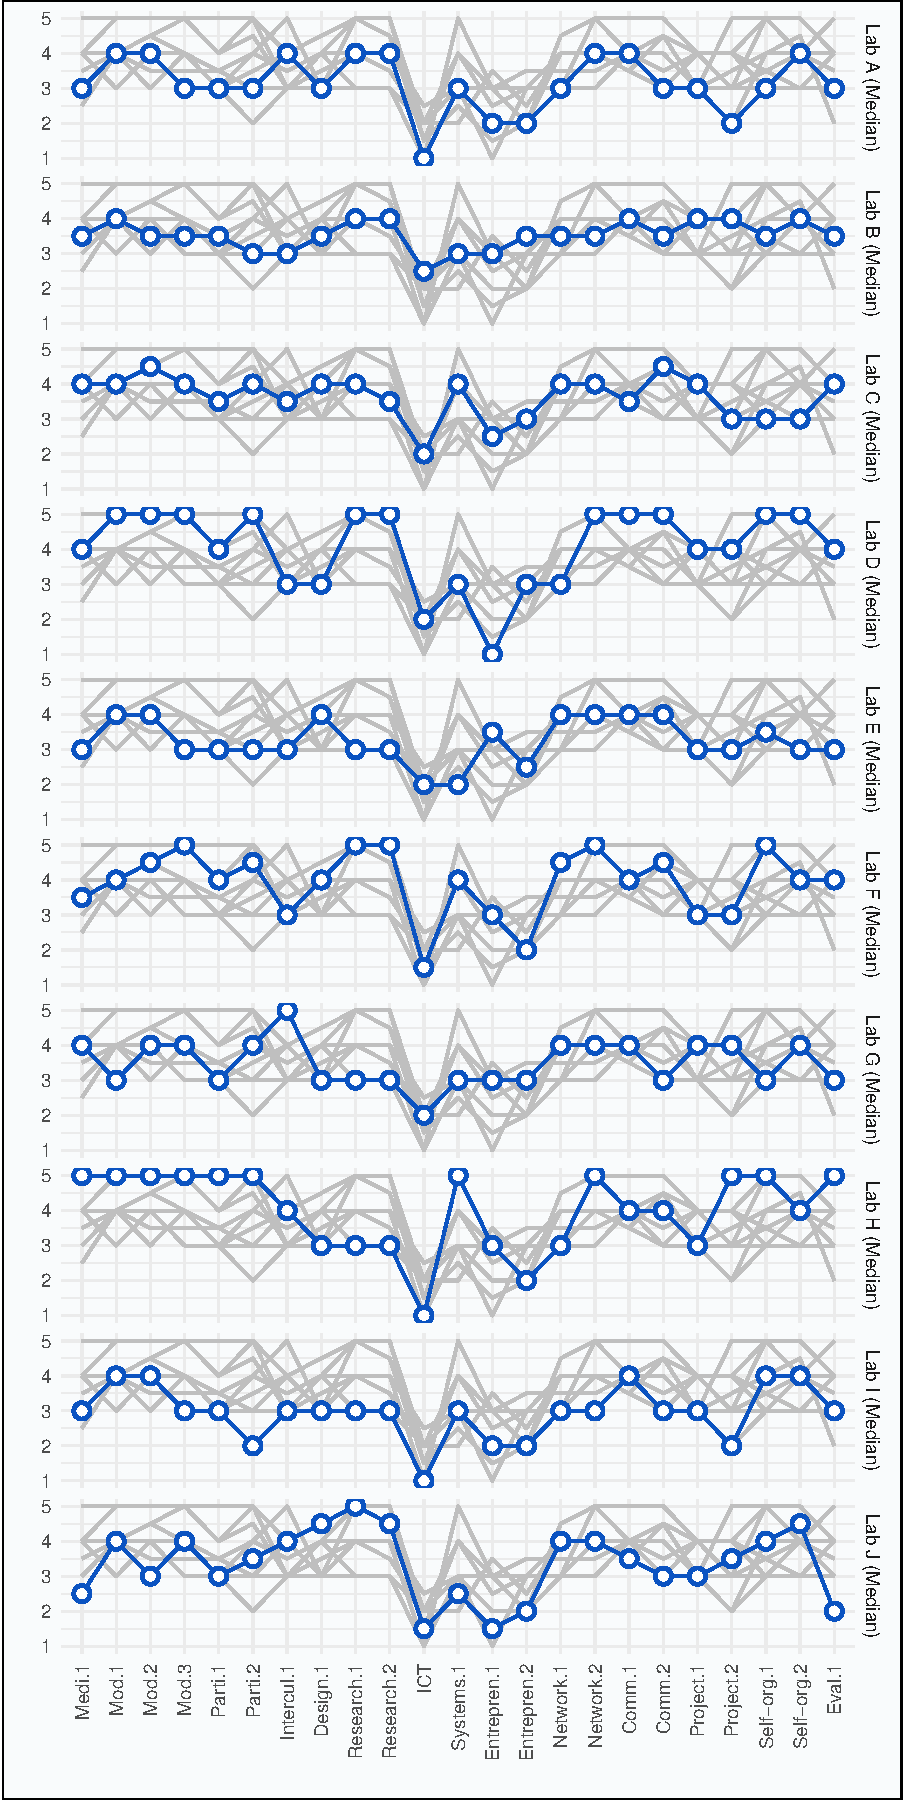
\includegraphics[width=0.7\linewidth]{index_files/figure-latex/unnamed-chunk-3-1} \end{center}

\bibliography{CAIM2021.bib}


\end{document}